% Options for packages loaded elsewhere
\PassOptionsToPackage{unicode}{hyperref}
\PassOptionsToPackage{hyphens}{url}
\PassOptionsToPackage{dvipsnames,svgnames,x11names}{xcolor}
%
\documentclass[
  11pt,
  numbers=noendperiod]{book}

\usepackage{amsmath,amssymb}
\usepackage{lmodern}
\usepackage{iftex}
\ifPDFTeX
  \usepackage[T1]{fontenc}
  \usepackage[utf8]{inputenc}
  \usepackage{textcomp} % provide euro and other symbols
\else % if luatex or xetex
  \usepackage{unicode-math}
  \defaultfontfeatures{Scale=MatchLowercase}
  \defaultfontfeatures[\rmfamily]{Ligatures=TeX,Scale=1}
\fi
% Use upquote if available, for straight quotes in verbatim environments
\IfFileExists{upquote.sty}{\usepackage{upquote}}{}
\IfFileExists{microtype.sty}{% use microtype if available
  \usepackage[]{microtype}
  \UseMicrotypeSet[protrusion]{basicmath} % disable protrusion for tt fonts
}{}
\makeatletter
\@ifundefined{KOMAClassName}{% if non-KOMA class
  \IfFileExists{parskip.sty}{%
    \usepackage{parskip}
  }{% else
    \setlength{\parindent}{0pt}
    \setlength{\parskip}{6pt plus 2pt minus 1pt}}
}{% if KOMA class
  \KOMAoptions{parskip=half}}
\makeatother
\usepackage{xcolor}
\usepackage[normalem]{ulem}
\setlength{\emergencystretch}{3em} % prevent overfull lines
\setcounter{secnumdepth}{5}
% Make \paragraph and \subparagraph free-standing
\ifx\paragraph\undefined\else
  \let\oldparagraph\paragraph
  \renewcommand{\paragraph}[1]{\oldparagraph{#1}\mbox{}}
\fi
\ifx\subparagraph\undefined\else
  \let\oldsubparagraph\subparagraph
  \renewcommand{\subparagraph}[1]{\oldsubparagraph{#1}\mbox{}}
\fi

\usepackage{color}
\usepackage{fancyvrb}
\newcommand{\VerbBar}{|}
\newcommand{\VERB}{\Verb[commandchars=\\\{\}]}
\DefineVerbatimEnvironment{Highlighting}{Verbatim}{commandchars=\\\{\}}
% Add ',fontsize=\small' for more characters per line
\usepackage{framed}
\definecolor{shadecolor}{RGB}{241,243,245}
\newenvironment{Shaded}{\begin{snugshade}}{\end{snugshade}}
\newcommand{\AlertTok}[1]{\scriptsize\textcolor[rgb]{0.68,0.00,0.00}{#1}}
\newcommand{\AnnotationTok}[1]{\scriptsize\textcolor[rgb]{0.37,0.37,0.37}{#1}}
\newcommand{\AttributeTok}[1]{\scriptsize\textcolor[rgb]{0.40,0.45,0.13}{#1}}
\newcommand{\BaseNTok}[1]{\scriptsize\textcolor[rgb]{0.68,0.00,0.00}{#1}}
\newcommand{\BuiltInTok}[1]{\scriptsize\textcolor[rgb]{0.00,0.23,0.31}{#1}}
\newcommand{\CharTok}[1]{\scriptsize\textcolor[rgb]{0.13,0.47,0.30}{#1}}
\newcommand{\CommentTok}[1]{\scriptsize\textcolor[rgb]{0.37,0.37,0.37}{#1}}
\newcommand{\CommentVarTok}[1]{\scriptsize\textcolor[rgb]{0.37,0.37,0.37}{\textit{#1}}}
\newcommand{\ConstantTok}[1]{\scriptsize\textcolor[rgb]{0.56,0.35,0.01}{#1}}
\newcommand{\ControlFlowTok}[1]{\scriptsize\textcolor[rgb]{0.00,0.23,0.31}{#1}}
\newcommand{\DataTypeTok}[1]{\scriptsize\textcolor[rgb]{0.68,0.00,0.00}{#1}}
\newcommand{\DecValTok}[1]{\scriptsize\textcolor[rgb]{0.68,0.00,0.00}{#1}}
\newcommand{\DocumentationTok}[1]{\scriptsize\textcolor[rgb]{0.37,0.37,0.37}{\textit{#1}}}
\newcommand{\ErrorTok}[1]{\scriptsize\textcolor[rgb]{0.68,0.00,0.00}{#1}}
\newcommand{\ExtensionTok}[1]{\scriptsize\textcolor[rgb]{0.00,0.23,0.31}{#1}}
\newcommand{\FloatTok}[1]{\scriptsize\textcolor[rgb]{0.68,0.00,0.00}{#1}}
\newcommand{\FunctionTok}[1]{\scriptsize\textcolor[rgb]{0.28,0.35,0.67}{#1}}
\newcommand{\ImportTok}[1]{\scriptsize\textcolor[rgb]{0.00,0.46,0.62}{#1}}
\newcommand{\InformationTok}[1]{\scriptsize\textcolor[rgb]{0.37,0.37,0.37}{#1}}
\newcommand{\KeywordTok}[1]{\scriptsize\textcolor[rgb]{0.00,0.23,0.31}{#1}}
\newcommand{\NormalTok}[1]{\scriptsize\textcolor[rgb]{0.00,0.23,0.31}{#1}}
\newcommand{\OperatorTok}[1]{\scriptsize\textcolor[rgb]{0.37,0.37,0.37}{#1}}
\newcommand{\OtherTok}[1]{\scriptsize\textcolor[rgb]{0.00,0.23,0.31}{#1}}
\newcommand{\PreprocessorTok}[1]{\scriptsize\textcolor[rgb]{0.68,0.00,0.00}{#1}}
\newcommand{\RegionMarkerTok}[1]{\scriptsize\textcolor[rgb]{0.00,0.23,0.31}{#1}}
\newcommand{\SpecialCharTok}[1]{\scriptsize\textcolor[rgb]{0.37,0.37,0.37}{#1}}
\newcommand{\SpecialStringTok}[1]{\scriptsize\textcolor[rgb]{0.13,0.47,0.30}{#1}}
\newcommand{\StringTok}[1]{\scriptsize\textcolor[rgb]{0.13,0.47,0.30}{#1}}
\newcommand{\VariableTok}[1]{\scriptsize\textcolor[rgb]{0.07,0.07,0.07}{#1}}
\newcommand{\VerbatimStringTok}[1]{\scriptsize\textcolor[rgb]{0.13,0.47,0.30}{#1}}
\newcommand{\WarningTok}[1]{\scriptsize\textcolor[rgb]{0.37,0.37,0.37}{\textit{#1}}}

\providecommand{\tightlist}{%
  \setlength{\itemsep}{0pt}\setlength{\parskip}{0pt}}\usepackage{longtable,booktabs,array}
\usepackage{calc} % for calculating minipage widths
% Correct order of tables after \paragraph or \subparagraph
\usepackage{etoolbox}
\makeatletter
\patchcmd\longtable{\par}{\if@noskipsec\mbox{}\fi\par}{}{}
\makeatother
% Allow footnotes in longtable head/foot
\IfFileExists{footnotehyper.sty}{\usepackage{footnotehyper}}{\usepackage{footnote}}
\makesavenoteenv{longtable}
\usepackage{graphicx}
\makeatletter
\def\maxwidth{\ifdim\Gin@nat@width>\linewidth\linewidth\else\Gin@nat@width\fi}
\def\maxheight{\ifdim\Gin@nat@height>\textheight\textheight\else\Gin@nat@height\fi}
\makeatother
% Scale images if necessary, so that they will not overflow the page
% margins by default, and it is still possible to overwrite the defaults
% using explicit options in \includegraphics[width, height, ...]{}
\setkeys{Gin}{width=\maxwidth,height=\maxheight,keepaspectratio}
% Set default figure placement to htbp
\makeatletter
\def\fps@figure{htbp}
\makeatother
\newlength{\cslhangindent}
\setlength{\cslhangindent}{1.5em}
\newlength{\csllabelwidth}
\setlength{\csllabelwidth}{3em}
\newlength{\cslentryspacingunit} % times entry-spacing
\setlength{\cslentryspacingunit}{\parskip}
\newenvironment{CSLReferences}[2] % #1 hanging-ident, #2 entry spacing
 {% don't indent paragraphs
  \setlength{\parindent}{0pt}
  % turn on hanging indent if param 1 is 1
  \ifodd #1
  \let\oldpar\par
  \def\par{\hangindent=\cslhangindent\oldpar}
  \fi
  % set entry spacing
  \setlength{\parskip}{#2\cslentryspacingunit}
 }%
 {}
\usepackage{calc}
\newcommand{\CSLBlock}[1]{#1\hfill\break}
\newcommand{\CSLLeftMargin}[1]{\parbox[t]{\csllabelwidth}{#1}}
\newcommand{\CSLRightInline}[1]{\parbox[t]{\linewidth - \csllabelwidth}{#1}\break}
\newcommand{\CSLIndent}[1]{\hspace{\cslhangindent}#1}

\makeatletter
\makeatother
\makeatletter
\@ifpackageloaded{bookmark}{}{\usepackage{bookmark}}
\makeatother
\makeatletter
\@ifpackageloaded{caption}{}{\usepackage{caption}}
\AtBeginDocument{%
\ifdefined\contentsname
  \renewcommand*\contentsname{Table of contents}
\else
  \newcommand\contentsname{Table of contents}
\fi
\ifdefined\listfigurename
  \renewcommand*\listfigurename{List of Figures}
\else
  \newcommand\listfigurename{List of Figures}
\fi
\ifdefined\listtablename
  \renewcommand*\listtablename{List of Tables}
\else
  \newcommand\listtablename{List of Tables}
\fi
\ifdefined\figurename
  \renewcommand*\figurename{Figure}
\else
  \newcommand\figurename{Figure}
\fi
\ifdefined\tablename
  \renewcommand*\tablename{Table}
\else
  \newcommand\tablename{Table}
\fi
}
\@ifpackageloaded{float}{}{\usepackage{float}}
\floatstyle{ruled}
\@ifundefined{c@chapter}{\newfloat{codelisting}{h}{lop}}{\newfloat{codelisting}{h}{lop}[chapter]}
\floatname{codelisting}{Listing}
\newcommand*\listoflistings{\listof{codelisting}{List of Listings}}
\makeatother
\makeatletter
\@ifpackageloaded{caption}{}{\usepackage{caption}}
\@ifpackageloaded{subcaption}{}{\usepackage{subcaption}}
\makeatother
\makeatletter
\@ifpackageloaded{tcolorbox}{}{\usepackage[many]{tcolorbox}}
\makeatother
\makeatletter
\@ifundefined{shadecolor}{\definecolor{shadecolor}{rgb}{.97, .97, .97}}
\makeatother
\makeatletter
\makeatother
\ifLuaTeX
  \usepackage{selnolig}  % disable illegal ligatures
\fi
\IfFileExists{bookmark.sty}{\usepackage{bookmark}}{\usepackage{hyperref}}
\IfFileExists{xurl.sty}{\usepackage{xurl}}{} % add URL line breaks if available
\urlstyle{same} % disable monospaced font for URLs
\hypersetup{
  pdftitle={Data Analysis in High-Energy Physics as a Differentiable Program},
  pdfauthor={Nathan Simpson},
  colorlinks=true,
  linkcolor={blue},
  filecolor={Maroon},
  citecolor={Blue},
  urlcolor={Blue},
  pdfcreator={LaTeX via pandoc}}

\title{Data Analysis in High-Energy Physics as a Differentiable Program}
\author{Nathan Simpson}
\date{02/03/2023}

%%%%%%%%%%%%%%%%%%%%%% LUND THESIS TEMPLATE
% Non-breakable hyphen. Use for things like "(re-)print". 
\newcommand\nobrkhyph{\mbox{-}}

% Small caps serif font, for Paper numbers, ISBN, etc
\newcommand{\I}{\textrm{\scshape i}\xspace}
\newcommand{\II}{\textrm{\scshape ii}\xspace}
\newcommand{\III}{\textrm{\scshape iii}\xspace}
\newcommand{\IV}{\textrm{\scshape iv}\xspace}
\newcommand{\V}{\textrm{\scshape v}\xspace}
\newcommand{\VI}{\textrm{\scshape vi}\xspace}
\newcommand{\VII}{\textrm{\scshape vii}\xspace}
\newcommand{\VIII}{\textrm{\scshape viii}\xspace}
\newcommand{\IX}{\textrm{\scshape ix}\xspace}
\newcommand{\X}{\textrm{\scshape x}\xspace}
\newcommand{\ISBN}{\textrm{\scshape isbn}\xspace}
\newcommand{\ISSN}{\textrm{\scshape issn}\xspace}

% Must come in the beginning. Changes the spacing in the table of contents to look more pleasing
\usepackage{tocloft}
\setlength{\cftbeforepartskip}{5.0mm}
\setlength{\cftbeforechapskip}{2.0mm}
\setlength{\cftbeforesecskip}{0.0mm}

% Must come in the beginning. To calculate the total number of pages
\usepackage{pageslts}

%%%%%%%%%%%%%%%%%%%%%%%%%% Everything font-related %%%%%%%%%%%%%%%%%%%%%%%%%%%%%%%%%%%%%%%
\usepackage{ifxetex}

% Font selections - they are only used when you compile with xelatex (strongly recommended). If you use 
% pdflatex, the default latex fonts will be used, you will break the University graphical profile, and your
% thesis will look much much uglier.

\ifxetex
	% \usepackage{mathspec}
	\usepackage[no-math]{fontspec}
	\usepackage{xunicode}
	\usepackage{xltxtra}
	% Adobe Garamond Pro for serif fonts and maths, Frutiger as sans, according to LU graphical profile
	% Tables get monospaced numerals, text gets proportional numerals, mathmode gets uppercase monospaced numberals
	% \setmainfont[Mapping=tex-text,Numbers={OldStyle,Proportional}]{Adobe Garamond Pro}
         \setmainfont{AGaramondPro}[
        Path = fonts/,
        Extension = .otf,
        UprightFont = *-Regular,
        BoldFont = *-Semibold,
        ItalicFont = *-Italic,
        Mapping = tex-text,
        Numbers = {OldStyle, Proportional}
        ]
	\AtBeginEnvironment{tabular}{\addfontfeatures{Numbers={Monospaced}}}
	% \setsansfont{Frutiger LT Std 45 Light}
	% \setmathfont(Greek,Digits,Latin){Adobe Garamond Pro}
	% mathspec is broken. The next eight lines work around that.
	% \usepackage{etoolbox}
	% \makeatletter
	% \begingroup\lccode`~=`"
	% \lowercase{\endgroup
	%   \everymath{\let~\eu@active@quote}
	%   \everydisplay{\let~\eu@active@quote}
	% }
	% \makeatother
\else
	% This is what is used for pdf latex. 
	% You can try \usepackage{ebgaramond} with (pdf)latex, however that does not have bold fonts ... !
	%\usepackage{ebgaramond}
	 \usepackage[utf8]{inputenc}
\fi
%%%%%%%%%%%% end font selections

% Support for greek (non-math non-italic) text, e.g. for units like mircometer: \textmu m 
% \usepackage{textgreek}

% Additional font sizes \HUGE and \ssmall, needed for figure captions
\usepackage{moresize}

% figure captions in bold (i.e. "Figure 1" in bold), sans serif, smaller font size, hanging label, always starting on the left side
\usepackage{subfig}
\DeclareCaptionFont{ssmall}{\ssmall}
\DeclareCaptionFont{tiny}{\tiny}% "scriptsize" is defined by floatrow, "tiny" not
\captionsetup{margin=0em,font={ssmall,sf},labelfont={bf},format=hang,singlelinecheck=false} 

% figures centred, smaller font in tables, captions on top for tables
\usepackage{floatrow}
% \DeclareFloatFont{tiny}{\tiny}% "scriptsize" is defined by floatrow, "tiny" not
% \DeclareFloatFont{ssmall}{\ssmall}
% \floatsetup[table]{font={footnotesize},position=top}
%%%%%%%%%%%%%%%%%%%%%%%%%%%%%%%%%%%% end fonts %%%%%%%%%%%%%%%%%%%%%%%%%%%%%%%%%%%%%%%%%%%%%%%%%%%%%%%

% For tables spanning the full text width
\usepackage{tabularx}

% For URLs use \url{<URL>}
\usepackage{url}

% Chapters should have numbers - a typical thesis consists of two chapters:
% One to introduce and summarize the research ("kappa"), and one for
% reproductions of the papers and manuscripts. No need to number them by default.
% If you need chapter numbers back, comment the following line.
% \renewcommand{\thesection}{\arabic{section}} 

% Sections and subsections have numbers, subsubsections etc do not.
\setcounter{secnumdepth}{3}

% Only chapters and sections appear in the table of contents, not subsections etc
\addtocontents{toc}{\protect\setcounter{tocdepth}{1}}

% Ensures that \cleardoublepage inserts empty pages without page number
\usepackage{emptypage} 

% For text macros (e.g., small caps macros)
\usepackage{xspace}

% For "Lorem Ipsum" style place holders
\usepackage{blindtext}

% For \includegraphics
\usepackage{graphicx}

% Nice looking tables with correct spacings 
\usepackage{booktabs}

% Tables spanning more than one page
\usepackage{longtable}
 
% Math symbols
\usepackage{amsfonts,amsmath,amssymb}

% To include the PDFs of the papers
\usepackage{pdfpages}

% For Natural Science students who use ADS. Save to have in any case.
% \usepackage{auxiliary_texfiles/aas_macros}

% Hyphenation, support for different languages, last one is default
% % Make sure to install the hyphenation packages for all languages you need
% \usepackage[swedish,ngerman,british]{babel} 

% Reference in style of Natural Sciences
\usepackage{natbib}

% Non-indented paragraphs with a small vertical space in-between
\parindent 0in
\parskip 3mm

% Paper size. Typically this works also fine when printed on A4 (text size is
% as print later, just the margins become wider to accommodate the too large
% sheets).
%% G5 format
% \usepackage[paperwidth=169mm,paperheight=239mm,total={13.3cm,19.6cm}, top=1.8cm, ignorehead, centering, footskip=\footskip+4mm ]{geometry}
% If you prefer E5 (smaller) you can use this line instead. Also go to frontmatter.tex and change the datasheet from G5 to E5.
%% E5 format
\usepackage[paperwidth=155mm,paperheight=220mm,total={12cm,18cm}, top=1.8cm, ignorehead, footskip=\footskip+4mm ]{geometry}

% not every page needs to go to the same bottom line. Allows nicer page breaks.
\raggedbottom

% avoid orphan/widow lines. Lower this number if necessary to get a good layout.
\widowpenalty500
\clubpenalty500


% These command should allow figures to be placed close to where we define them, 
% thus we can influence the figure placement to some extent.
%% min page fraction that must be filled with text
% \renewcommand{\textfraction}{0.1} 
\renewcommand{\textfraction}{0.}
%% max page fraction that a float may take at the top of the page
%\renewcommand{\topfraction}{0.9} 
\renewcommand{\topfraction}{1.0}
%% max page fraction that a float may take at the bottom of the page
%\renewcommand{\bottomfraction}{0.9}
\renewcommand{\bottomfraction}{1.0}
%% max page fraction that may be filled with floats
%\renewcommand{\floatpagefraction}{0.5}
\renewcommand{\floatpagefraction}{1.0}
%% maximum number of floats at the top of the page
\setcounter{topnumber}{3}
%% maximum number of floats at the bottom of the page
\setcounter{bottomnumber}{1}
%% maximum total number of floats on a page
\setcounter{totalnumber}{3}

% Figures can be kept in the same directory as the thesis, or in a Figure/
% directory, without need to specifying which of the two it is
\graphicspath{{Figures/}}


%%%%%%%%%%%%%%%%%%%%%%%%%%%%%%%%%%%%%%%%%%%%%%%%%%%%%%%%%%%%%%%%%%%%
% define commands for chapters, sections, and subsections that do not 
% have a number, but are entered as candidates for the table of contents.
\newcommand\chap[1]{%
  \chapter*{#1}%
  \addcontentsline{toc}{chapter}{#1}
  \markboth{#1}{#1}
}
\newcommand\sect[1]{%
  \section*{#1}%
  \addcontentsline{toc}{section}{#1}
  \markright{#1}
}
\newcommand\subsect[1]{%
  \subsection*{#1}%
  \addcontentsline{toc}{subsection}{#1}
}


%%%%%%%%%%%%%%%%%%%%%%%%%%%%%%%%%%%%%%%%%%%%%%%%%%%%%%%%%%%%%%%%%%%%
% Define nice headers and footers
% To keep the thesis non-cluttered we only put the page number into the footer,
% and avoid headers
\usepackage{fancyhdr}
\fancyheadoffset{0cm}
\pagestyle{plain}
%page number in the foot centre 
\cfoot{\fancyplain{\thepage}{}}

% You want to use headers? Here is some things for your inspiration:
%\renewcommand{\chaptermark}[1]%
%               {\markboth{#1}{#1}}
%\renewcommand{\sectionmark}[1]%
%               {\markright{\thesection\ #1}}
%\renewcommand{\chaptermark}[1]{\markboth{\thechapter\ #1}{\thechapter\ #1}}
%\lhead[\fancyplain{}{\thepage}]%
%      {\fancyplain{}{\textsl\rightmark}}
%\rhead[\fancyplain{}{\textsl\leftmark}]%
%      {\fancyplain{}{\thepage}}
% Contents and references should not print a uppercase header on their second pages
%\usepackage{etoolbox}
%\patchcmd{\tableofcontents}{\MakeUppercase\contentsname}{\contentsname}{}{}
%\patchcmd{\tableofcontents}{\MakeUppercase\contentsname}{\contentsname}{}{}
%\patchcmd{\bibsection}{\MakeUppercase{\bibname}}{\bibname}{}{}
%\patchcmd{\bibsection}{\MakeUppercase{\bibname}}{\bibname}{}{}

% References should be a section of the summary text, with number and all ...
\renewcommand\bibsection{\section{\bibname}\markright{\bibname}}

% If you want to use a box to summarize your papers, try \begin{thesisbox}{title}
\usepackage{tcolorbox}
\tcbuselibrary{skins}
\newtcolorbox{thesisbox}[2][]{
oversize=-2.5cm,
  enhanced,
  attach boxed title to top left={yshift=-2ex,xshift=6ex},
  before skip=1em,
  after skip=1em,
  colframe=black,
  colback=white,
  fonttitle=\bfseries, 
  colbacktitle=white,
  coltitle=black,
  boxed title style={
    boxrule=0pt,
    colframe=white,
    },
  title=#2,
  #1}


% ********************************************************************
% Re-usable information (title page, datasheet)
\newcommand{\myName}{Nathan Simpson}
\newcommand{\myYear}{2023}
\newcommand{\myMainTitle}{Data Analysis in High-Energy Physics as a Differentiable Program}

% Compact combination of combining title and subtitle, used in datasheet and as
% chapter title for the main part.
\newcommand{\myTitle}{\myMainTitle} 

\newcommand{\myFaculty}{Faculty of Physics}
\newcommand{\myDepartment}{Department of Particle Physics}
\newcommand{\myAddress}{Box 118\\SE--221 00 LUND\\Sweden} % Three lines maximum!

% Only change once you are ready. Looks to scary otherwise.
% This might be the degree you are obtaining: Thesis for the degree of Doctor of Philosophy
\newcommand{\myDegree}{Thesis for the degree of Doctor of Philosophy}
\newcommand{\myAdvisors}{Prof.~Else~Lytken, Dr.~Caterina~Doglioni}
\newcommand{\myOpponent}{Dr.~Luca~Lista}

\newcommand{\myDefenceAnnouncement}{%
	To be presented, with the permission of the
	\myFaculty\xspace of Lund University, for public criticism in the Rydberg
	lecture hall at the \myDepartment\xspace
	on Friday, the 3rd of February \myYear\xspace at 13:15. }
\newcommand{\myCoverBack}{%
	{\bf Cover illustration back:} 
	A pattern I generated while playing with the ``Gaussian firework'' referenced in the thesis work. Many thanks to \texttt{matplotlib} for enabling my graphic adventures over these four years, in every sense of the word.}
\newcommand{\myCoverFront}{%
	{\bf Cover illustration front:} The result from training a neural network to optimize both discovery and exclusion significances at once. Signal points are in teal, background in orange, and background up/down variations in red/gold. The contour lines are the decision boundaries of the neural network, which has learned to wrap around the signal by picking up knowledge of the systematic variations. }
\newcommand{\myFundingInformation}{%
	{\bf Funding information:} 
	The thesis work was financially supported by Insights, which is funded by the European Union’s Horizon 2020 research and innovation programme, call H2020-MSCA-ITN-2017, under Grant Agreement n. 765710. The last year of funding came from the Swedish Research Council via Lund University.}

% Series number. Astronomy users:
% Series: {\scshape lunfd6/(nfas}-1048)/1-\myPages/(\myYear)}
% where you increment the number 1048 by one wrt to last thesis at the department
% 
% Your department maybe uses something else, probably an ISSN number? 
% \newcommand{\mySeries}{%
% 	\ISSN: $<$ISSN number$>$}

\newcommand{\myISBNprint}{978-91-8039-493-2}
\newcommand{\myISBNpdf}{978-91-8039-494-9}
\newcommand{\myFormSignDate}{-7-4}

% total page number is computed automatically:
\newcommand{\myPages}{\lastpageref{LastPages}}

\newcommand{\myFormDefenceDate}{2023-02-03}
\newcommand{\myFormKeywords}{%
	differentiable programming, particle physics, statistical inference, machine learning}

% Write a short english abstract of the thesis here, goes into the data sheet page 4. 
\newcommand{\myAbstract}{
Machine learning methods are now ubiquitous in physics, but often target objectives that are one or two steps removed from our physics goals. A prominent example of this is the discrimination between signal and background processes, which doesn’t account for the presence of systematic uncertainties -- something crucial for the calculation of quantities such as the discovery significance and upper limits.

To combat this, this thesis shows that physics analysis workflows can be optimized in an end-to-end fashion, including the treatment of nuisance parameters that model systematic uncertainties, provided that the workflow is differentiable. By leveraging automatic differentiation and surrogates for non-differentiable operations, this work has made this possible for the first time, and demonstrates its use in a proof-of-concept scenario.

This thesis will motivate the use of end-to-end optimization as described above, cover the techniques that make it possible, and show recent developments in a high-energy physics context. Future directions that aim to scale and apply these methods will also be highlighted.

In addition to this, a method to interpolate between the signatures of new physics models is presented, which uses normalizing flows. The thesis then goes on to show the use of the technique in a search for a new scalar boson $S$ produced in association with a Higgs boson from a heavy new scalar $X$. There are also some contributions that interpolate between the event yields with Gaussian processes, and that show how we can use normalizing flows to construct a likelihood ratio-inspired observable.
}%

%%%%%%%%%%%%%%%%%%%%%%%%%%%%%%%%%%%%%%%%%%%


\begin{document}

%%%%%%%%%%%%% First pages with thesis title etc %%%%%%%%%%%%%%%%%%%%%%%%%%%%%%%%
% First six pages are contained in a separate file. Normally you should not
% need to edit it.
% This file contains the layout of the first six pages and the explanation text
% of a compilation thesis. 

%%%%%%%%%%%%% FIRST PAGES WITH THESIS TITLE ETC %%%%%%%%%%%%%%%%%%%%%%%%%%%%%%%%
% \frontmatter % roman numbers

% Page one: Title only
\thispagestyle{empty} % no page number
\begin{center}
\vspace*{5cm}
{\Large \myMainTitle}
%\\
%{\large \mySubTitle}
\end{center}

% Page two: empty. Empty space is important

%%%%%%%%%%%%%%%%%%%%%%%%%%%%%%%%%%%%%%%%%%%%%%%%%%%%%%%%%%%%%%%%%%%%%%%
% Page three: title page with small text (spikningsblad)

\cleardoublepage
\thispagestyle{empty} % no page number
~
\vfill
\begin{center}
{\HUGE \myMainTitle}
\\[2mm]
{\huge \mySubTitle}

\vfill
{by \myName}

\vfill
% black and white (default):
\includegraphics[width=0.25\textwidth]{LundUniversity_C2line_BLACK.eps}

\vspace{10mm}
{\large \myDegree}\\
{\large Thesis advisors: \myAdvisors}\\
{\large Faculty opponent: \myOpponent}\\
\vspace{1cm}
{\footnotesize
\myDefenceAnnouncement
}
\\
\end{center}
\vfill

%%%%%%%%%%%%%%%%%%%%%%%%%%%%%%%%%%%%%%%%%%%%%%%%%%%%%%%%%%%%%%%%%%%%%%%
% Page four: data sheet
\newpage \thispagestyle{empty} % no page number
%Either include datasheet texfile (will be filled in automatically), or a pdf
%containing datasheet (text needs to be already in it, edit
%sheetPDF_editable.pdf). Use one of the next two lines: 
\newcounter{aformdx}
\newcounter{aformdy}
\newcounter{aformx}
\newcounter{aformy}
\newcounter{aformtx}
\newcounter{aformtdx}
\newcounter{aformty}
\def\aformw{358}
\def\aformwhalf{\aformw / 2}
\def\aformwquart{\aformw / 4}
\def\aformwthreeq{\aformw / 4 * 3}
\def\aformh{517}
\def\aformb{23}
\def\aformlinew{0.4pt}
\def\aformrowh{20}
\def\aformRowh{24}
\newcommand\aformhline
{\put(\value{aformx},\value{aformy}){\line(1,0){\value{aformdx}}}}
\newcommand\aformvline
{\put(\value{aformx},\value{aformy}){\line(0,-1){\value{aformdy}}}}
\newcommand\aformvlinec
{\put(\value{aformx},\value{aformy}){\line(0,-1){16.25}}}
\newcommand\aformboxbase[5]
{
  \setcounter{aformtx}{\value{aformx}}
  \setcounter{aformtdx}{\value{aformdx}}
  \setcounter{aformty}{\value{aformy}}
  \addtocounter{aformtx}{#1}
  \addtocounter{aformtdx}{-#2}
  \addtocounter{aformty}{-#3}
  \put(\value{aformtx},\value{aformty})
  {
    \parbox[t]{\value{aformtdx}pt}
    {{\sf\tiny #4}{\scriptsize #5\par}}
  }
}
\newcommand\aformbox[2]{\aformboxbase{2}{11}{8}{#1}{#2}}
\newcommand\aformBox[2]{\aformboxbase{2}{11}{8}{#1}{#2}}

\begin{center}
\begin{picture}(\aformw,542)(0,0)
\linethickness{\aformlinew}
\put(0,\aformb){\framebox(\aformw,\aformh){}}
\put(-14,200){\rotatebox{90}{\parbox{200pt}
{\sf\tiny
DOKUMENTDATABLAD
enl SIS 61 41 21\\
}}}
\setcounter{aformx}{0}
\setcounter{aformy}{\aformb}
\addtocounter{aformy}{\aformh}
\setcounter{aformdx}{\aformwhalf}
\aformbox{Organization}
{\\
{\bf LUND UNIVERSITY}\vspace{0.1cm}
\\
{\myDepartment\\
\myAddress}
}
\setcounter{aformdy}{\aformrowh}
\addtocounter{aformdy}{\aformrowh}
\addtocounter{aformdy}{\aformrowh}
\addtocounter{aformdy}{\aformRowh}
\setcounter{aformx}{\aformwhalf}
\aformvline
\setcounter{aformx}{0}
\addtocounter{aformy}{-\aformrowh}
\addtocounter{aformy}{-\aformrowh}
\addtocounter{aformy}{-\aformRowh}
\aformbox{Author(s)}{\\\myName}
\setcounter{aformdy}{\aformrowh}
\aformhline
\addtocounter{aformy}{\aformrowh}
\addtocounter{aformy}{\aformrowh}
\addtocounter{aformy}{\aformRowh}
\setcounter{aformx}{\aformwhalf}
\aformbox{Document name}{\\{\bf DOCTORAL DISSERTATION}}
\addtocounter{aformy}{-\aformrowh}
\aformhline
\aformbox{Date of disputation}{\\\myFormDefenceDate}
\setcounter{aformx}{\aformwhalf}
\aformhline
\addtocounter{aformy}{-\aformrowh}
\addtocounter{aformdy}{\aformRowh}
\aformbox{Sponsoring organization}{}
\aformhline
\addtocounter{aformy}{-\aformRowh}
\addtocounter{aformy}{-\aformrowh}
\setcounter{aformx}{0}
\setcounter{aformdx}{\aformw}
\aformhline
\aformbox{Title and subtitle }{\\\myTitle}
\addtocounter{aformy}{-\aformRowh}
\setcounter{aformx}{0}
\aformhline
\aformBox{Abstract}
{\\
{\parskip0pt\parindent1em
\myAbstract
}
}
\setcounter{aformy}{\aformb}
% Correspond to one minus each in the bottom section
\addtocounter{aformy}{\aformRowh}
\addtocounter{aformy}{\aformRowh}
\addtocounter{aformy}{\aformRowh}
\addtocounter{aformy}{\aformRowh}
\addtocounter{aformy}{\aformrowh}
\addtocounter{aformy}{\aformrowh}
\addtocounter{aformy}{10}
\addtocounter{aformy}{10}
\aformhline
\aformbox{Key words}
{
\\\myFormKeywords
}
\addtocounter{aformy}{-\aformRowh}
\addtocounter{aformy}{-10}
\aformhline
\aformbox{Classification system and/or index terms (if any)}{}
\addtocounter{aformy}{-\aformRowh}
\aformhline
\aformbox{Supplementary bibliographical information}{}
\setcounter{aformx}{\aformwthreeq}
\setcounter{aformdx}{\aformwquart}
\setcounter{aformdy}{\aformRowh}
\aformvline
\aformbox{Language}{\\English}
\addtocounter{aformy}{-\aformRowh}
\setcounter{aformx}{0}
\setcounter{aformdx}{\aformw}
\aformhline
\aformbox{ISSN and key title}{}
\setcounter{aformx}{\aformwthreeq}
\addtocounter{aformdy}{10}
\aformvline
\addtocounter{aformdy}{-10}
\aformbox{ISBN}{\\\myISBNprint\xspace(print)\\\myISBNpdf\xspace(pdf)}
\addtocounter{aformy}{-\aformRowh}
\addtocounter{aformy}{-10}
\setcounter{aformx}{0}
\aformhline
\aformbox{Recipient's notes}{}
\setcounter{aformx}{\aformwhalf}
\setcounter{aformdy}{\aformrowh}
\addtocounter{aformdy}{\aformrowh}
\aformvline
\aformbox{Number of pages}{\\\myPages}
\setcounter{aformx}{\aformwthreeq}
\aformbox{Price}{}
\setcounter{aformdy}{\aformrowh}
\aformvline
\addtocounter{aformy}{-\aformrowh}
\setcounter{aformx}{\aformwhalf}
\setcounter{aformdx}{\aformwhalf}
\aformhline
\aformbox{Security classification}{}
\setcounter{aformx}{0}
\setcounter{aformdx}{\aformw}
\addtocounter{aformy}{-\aformrowh}
\addtocounter{aformy}{-4}
\aformbox{}
{\scriptsize I, the undersigned, being the copyright owner of the abstract of the
above-mentioned dissertation, hereby grant to all reference sources
the permission to publish and disseminate the abstract of the
above-mentioned dissertation.
}
\addtocounter{aformy}{-\aformRowh}
\addtocounter{aformy}{-20}
\aformbox{
\hspace{0pt}
%\put(44,1){\includegraphics{images/signature}} %Media-Tryck does not want this to be included as a graphic
}{}
\aformbox{\rm
\scriptsize
Signature \underline{\hskip 140pt}\hfill Date \underline{\hskip 80pt}
}{}
\addtocounter{aformy}{1}
\aformbox{}{\hskip 280pt \scriptsize \myFormSignDate}
\end{picture}
\end{center}

%\addtocounter{pages}{1} 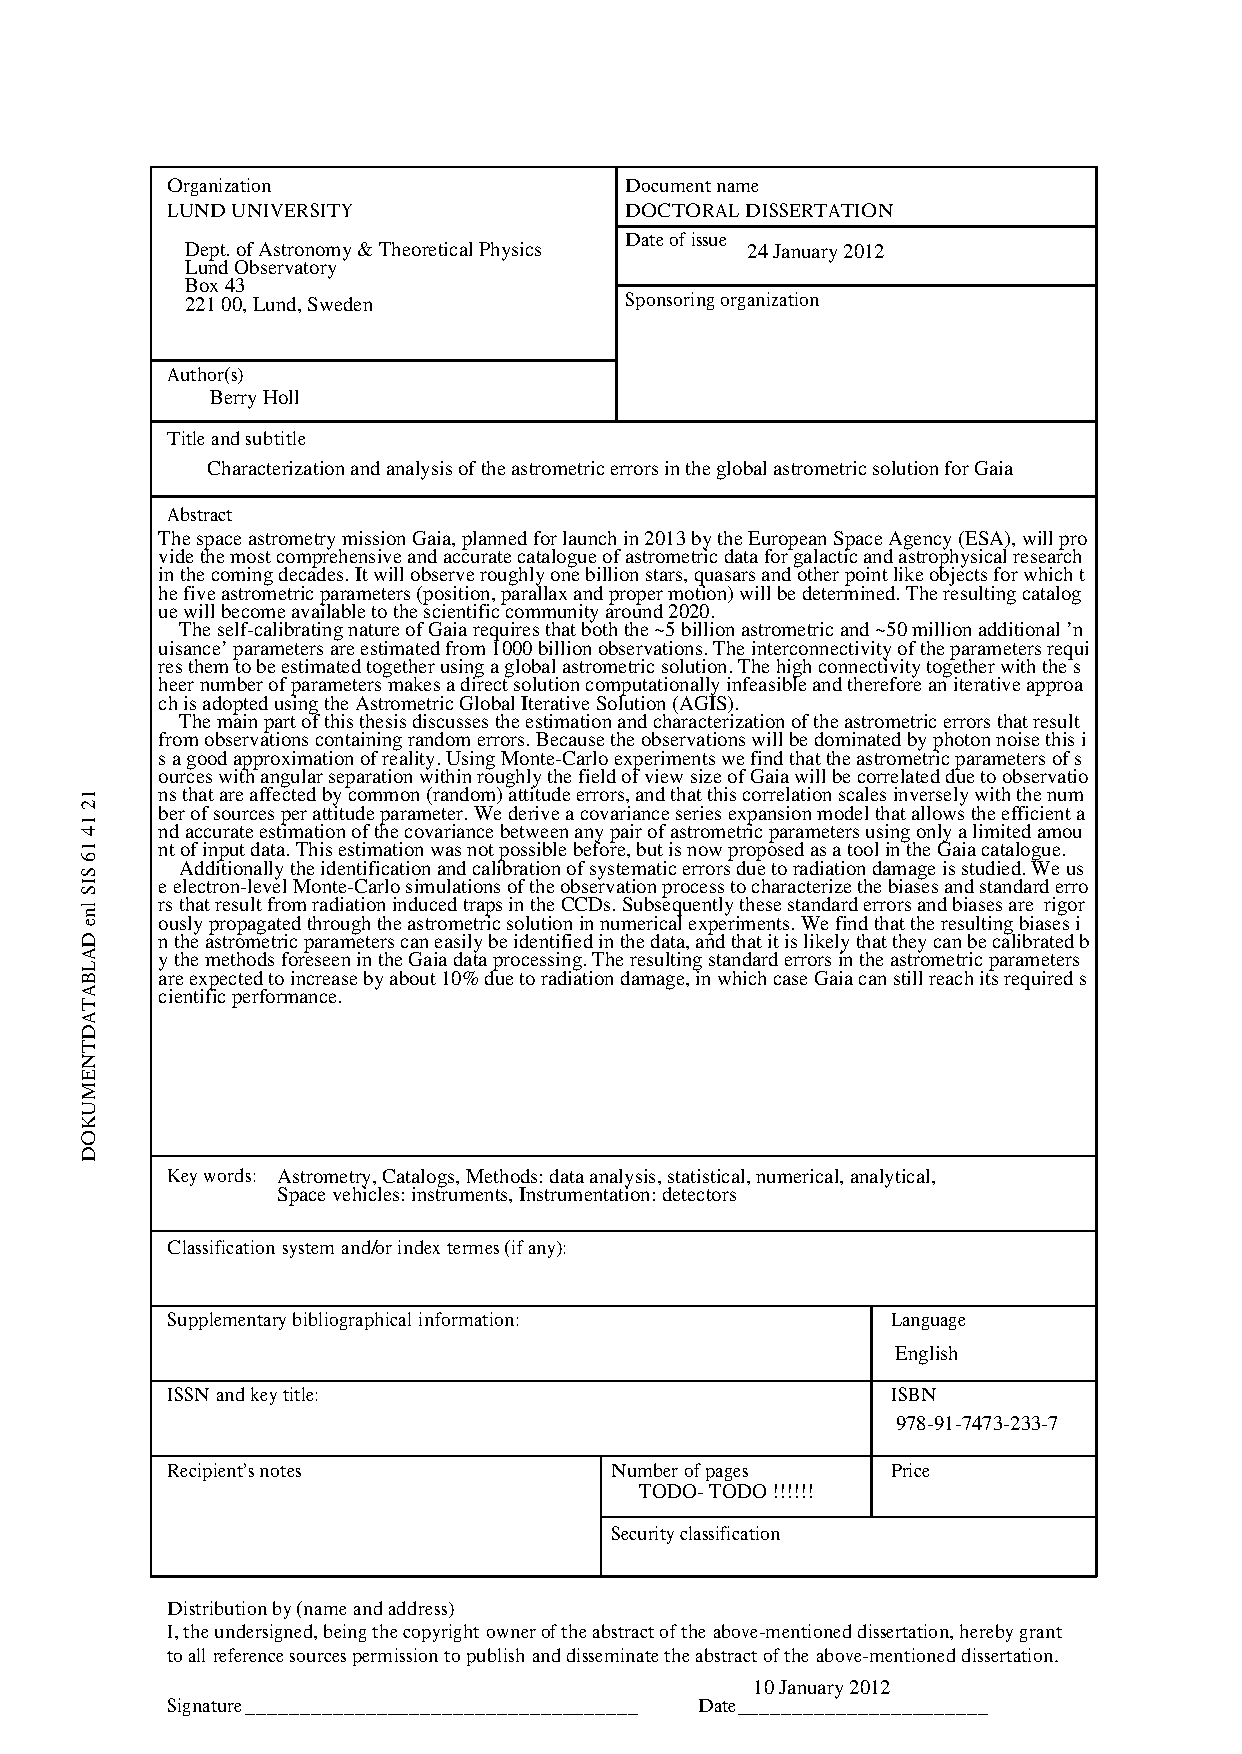
\includepdf[pages=1-1]{datasheetPDF_editable}

%%%%%%%%%%%%%%%%%%%%%%%%%%%%%%%%%%%%%%%%%%%%%%%%%%%%%%%%%%%%%%%%%%%%%%%
% Page five: title and author, without small text. Looks good!

\cleardoublepage
\thispagestyle{empty} % no page number
~
\vfill
\begin{center}
{\HUGE \myMainTitle}
\\[2mm]
{\huge \mySubTitle}

\vfill
{by \myName}

\vfill
% black and white (default):
\includegraphics[width=0.25\textwidth]{LundUniversity_C2line_BLACK.eps}

% Colour text in white so that the spacing is the same as on page three, but with less clutter
\color{white}{
\vspace{10mm}
{\large \myDegree}\\
{\large Thesis advisors: \myAdvisors}\\
{\large Faculty opponent: \myOpponent}\\
\vspace{1cm}
{\footnotesize
\myDefenceAnnouncement
}
}
\\
\end{center}
\vfill


%%%%%%%%%%%%%%%%%%%%%%%%%%%%%%%%%%%%%%%%%%%%%%%%%%%%%%%%%%%%%%%%%%%%%%%
% Page six: Cover image description, ISBN, copyright
\newpage 
\thispagestyle{empty} % no page number
%~
%\vfill
\vspace{-15mm}
A doctoral thesis at a university in Sweden takes either the form of a single,
cohesive research study (monograph) or a summary of research papers
(compilation thesis), which the doctoral student has written alone or together
with one or several other author(s). 

In the latter case the thesis consists of two parts. An introductory text puts
the research work into context and summarizes the main points of the papers.
Then, the research publications themselves are reproduced, together
with a description of the individual contributions of the authors. The
research papers may either have been already published or are manuscripts at
various stages (in press, submitted, or in draft). 

\vfill
{\small
\myCoverFront\\
\\
\myCoverBack\\
\\
\myFundingInformation


\vspace{5mm}
\copyright\, \myName~\myYear\\
\\
\myFaculty, {\myDepartment}
\\
\\
\ISBN: \myISBNprint~(print)\\ % ISBN av svenska ISBN centralen
\ISBN: \myISBNpdf~(pdf)\\ % ISBN av svenska ISBN centralen
\mySeries\\
\\
Printed in Sweden by Media-Tryck, Lund~University, Lund~\myYear


\includegraphics[width=0.5\textwidth]{ENG-Miljologotyper-sid-2-BLACK.eps}
}


% ===============================================================
% ===================== INSPIRATIONAL QUOTE:  ===================
% ===============================================================
\newpage
\thispagestyle{empty} % No page number on quote page
~
\vspace{140pt}
\begin{flushright}
\textit{To family by birth,\\family found,\\and myself.}
\end{flushright}

\newpage
\thispagestyle{empty} % No page number on quote page

\section*{Acknowledgements}

Oh gosh, where to even start. This has been quite the ride for me, and I feel the need to somehow jot down every detail of self-discovery that I've accumulated as a result of everything that's happened over my three years in Sweden (+ 6 months in Geneva at CERN). I'll spare you that, and just give the people that were involved their share of due thanks.

First, I want to acknowledge my Grandad, who passed away from cancer in the final year of my PhD, right before I started writing this thesis. Despite having no physics background, he would have read the whole thing cover-to-cover in his own diligent way, and would have jubilantly and sincerely given me credit for it all the while. His words of ``Enjoy it man'' that he told me when I was about to move here still echo in my mind, and I like to think I did my best to embrace that within my capabilities to do so. I'm going to pass on that sentiment to you, the reader: whatever you're doing in life right now, enjoy it. However you can.

Now, I'll do my best to give my heartfelt love and credit to as many of the people that have been with me along the way that I remember while writing this.

\textit{Alvaró,} for all the fun adventures and sushi sessions over my years in Lund. Also to \textit{Anna} for all your fantastic references and queer anecdotes. Special thanks go the revolving door of a collective that is Winstrup, who's occupants have always been endlessly kind and loving. This was certainly the closest thing to a second home I had in Lund (I was eventually referred to affectionately as ``furniture'').

\textit{Léopoldine}, for both enabling me and challenging me over the years. Your headstrong attitude to life and ability to love freely without judgement continually inspires me.

\textit{Anna-Mòntserrat}, for being someone that makes it completely effortless to be myself around, and for giving me boundless emotional support during all my crises.

\textit{Emma and Gunnar}, for somehow being instantly close friends from the moment I met you. Hanging out with you has truly done wonders to lift my spirits as I've been writing this.

\textit{Sean}, for being fantastic company at CERN, a guiding light in my pursuit of physics/machine learning, and the best yoga accountability partner a person could ask for. I then of course need to extend thanks to Yoga with Adriene for being a source of sanity, self-discovery, and stillness. 

On the topic of CERN, I need to also thank the whole ``noonch'' crew that facilitated so many fun times, including \textit{Mason}, \textit{Melissa}, \textit{Emily}, \textit{Nicole}, \textit{Max}, \textit{Rachel}, and many others that I'm sure I'm forgetting.

\textit{Lukas}, for being my informal supervisor over these years that helped turn a secondment into my main PhD topic by virtue of Twitter. Our debugging sessions in R1 were foundational to the way I approach programming and problem solving in general.

\textit{Matthew Feickert}, for being unbelievably supportive and generous with your expertise, friendship, and kindness. You are a role model for me in the way in which you bring others up around you, and are always patient and thoughtful when answering questions.

\textit{Giordon}, for helping me hack away at \texttt{pyhf}, and for the great time in Lund going through the intricacies of sign language.

\textit{Alex Held}, for providing me with a ridiculous amount of help via Slack, and for the awesome conversations at conferences over the times I've managed to bump into you. May your yields never be negative.

My supervisors \textit{Else} and \textit{Caterina}, for being patient with all the admin for one, and for both enabling my blossoming into an independent researcher in your very different ways.

All my Lund colleagues, both past and present: \textit{Eva} for rescuing me in Copenhagen with a game of Mia, and for all the critical takes on Taylor's albums; \textit{Katja}, for being a total hero for the TRT, letting me beat you at Soul Calibur, and being one of my biggest inspirations as a PhD student through your resilience; \textit{Alex} for being superb company and breathing life into the division by virtue thereof; \textit{Erik} for being a staunch supporter of my rare Twitch adventures (\texttt{twitch.tv/phi\_nate}); \textit{Hannah} for being the other horse in our tornado of a two-person carousel, and for the therapy sessions disguised as `improv'; \textit{Florido} and \textit{Bozena}, who between them had to put up with me ordering all sorts of weird equipment; and all the many others. I hope Partikelfysik retains its familial feel after the 2023 merge.

\newpage

\textit{Melissa Franklin}, for being just about the limit of how much anarchical inspiration as a physicist one can cram into a humanoid form. Your company at Lund is always a pleasant memory when it surfaces.

Everyone in the IRIS-HEP Slack, which was an unbelievable crutch to lean on for physics, statistics, and programming help. I'll do my best to pass on the kindness I received here.

The people in \textit{INSIGHTS}, which is the training network that I was part of during my PhD. So many to name: \textit{Artem}, \textit{Hevjin}, \textit{Sitong}, \textit{Rahul}, \textit{Pim}, \textit{Lukas}, \textit{Viktor}, \textit{Vasil}, \textit{Daria}. Also to all the PIs for hosting such great training events, from which I learned so much of the content relevant for this thesis.

My immediate family: \textit{Mum and Dad} for your endless love and support in so many ways; my brother \textit{Matthew} for all the zigs, zogs, music, and duels; my sister \textit{Gemma} for all the fun Australian phonecalls; her fiancé \textit{Connor}, for all the gym classes when I came to visit, and the emergency drive to the airport for a COVID test at near-light speed; and my \textit{Gran} for many of her warm-hearted gestures, even through such a tumultuous time.

My sports friends over at LUGI tennis and badminton, for literally keeping me in one piece while writing. Genuinely couldn't have survived otherwise.

The staff at the two opposing Espresso House franchises by Lund Centralen, where alternating between them became the only significant variation between my days while I wrote my thesis. Thanks also to the barista \textit{Jonas}, who made a special effort to be a familiar presence.

Whew, that's all that I've got in me. I love you all.

\cleardoublepage
%%%%%%%%%%%%%%%%%%%%%%%%%%%%%%%%LUND


\ifdefined\Shaded\renewenvironment{Shaded}{\begin{tcolorbox}[frame hidden, breakable, borderline west={3pt}{0pt}{shadecolor}, boxrule=0pt, enhanced, interior hidden, sharp corners]}{\end{tcolorbox}}\fi

\renewcommand*\contentsname{Table of contents}
{
\hypersetup{linkcolor=}
\setcounter{tocdepth}{2}
\tableofcontents
}
\bookmarksetup{startatroot}

\hypertarget{preface}{%
\chapter*{Preface}\label{preface}}
\addcontentsline{toc}{chapter}{Preface}

\begin{quote}
``I didn't have time to write a short \sout{letter} thesis, so I wrote a
long one instead.'' -- Mark Twain (adapted)
\end{quote}

Many curious things can stem from direct messages on Twitter\footnote{Citation needed, but not provided.}. You
can count the contents of this thesis as one of them.

In October of 2019, I got off the tram from the Blandonnet stop in
Geneva, arriving bewildered to CERN for a 6 month placement. I had no
idea what I was going to be doing there, since my assigned supervisor
and I had not communicated at any point leading up to this visit. I just
knew that I was doing this placement as part of my position, which was
funded as part of a Marie Curie International Training Network (they let
you do placements), and that my supervisor was in some way connected to
the team working on the \href{https://root.cern.ch}{ROOT software suite}.

Now, ROOT is sometimes talked about with a negative tone in high-energy
physics circles due to its steep learning curve and monolithic software
design. I will endeavour to do no such thing here, as this software was
a revolution in computing for its time, and continues to power the
majority of data analysis done at the Large Hadron Collider. However,
this is specialist software, and it is very much the case that the
typical undergraduate/masters student will likely have no training on
how to use it, which can significantly hinder the ability to play with
your code and understand what's going on. Moreover, many courses at
university will be teaching students to have proficiency with more
standard scientific analysis tools, such as the \href{}{scientific
Python ecosystem}. Being one of these people, I was keen to explore to
what extent I could utilize these tools that I had some familiarity with
in order to do my physics work. This led to me tweeting out about ROOT-less analysis, to which I got the response below, a
mere two months before my placement:

\begin{quote}
    pyhf is being used in a few on-going projects within ATLAS, also people
like e.g.~uproot for ntuple analysis. Complete end-to-end is difficult
since reading xAOD in uproot natively isn\textquotesingle t easy to
achieve (also need C++ CP tools etc). I\textquotesingle m happy to
help/collaborate!

\hfill--- \textit{Lukas Heinrich} (August 21, 2019)
\end{quote}


I enthusiastically followed up on Lukas' offer to collaborate, and
before I knew it, I was sat at a table in CERN's main restaurant (R1 if
you're a cool kid) with both Lukas and my would-be supervisor (who would
not be my supervisor), ready to start a project on building something
that had never been done before, but using tools that I was familiar
with. That project became \texttt{neos}, and started the development of
a new paradigm for how we view optimizing our data analysis pipelines,
and the cornerstone of this thesis -- differentiable programming.
Totally different from just a ROOT-less analysis, but I also did a bit
of that in the end anyway.

As such, if you were expecting a typical HEP thesis, you may be
surprised at what lies ahead, hopefully in a positive matter. We will
still traverse the lands of particle physics, but will be stepping
around many puddles that most dive into, and instead spend a bit of
extra time in the marshlands of probability and statistics, which inform
almost all of the work done in my PhD from a practical and motivational
standpoint. From there, we'll foray into the fields of gradients,
including how we calculate them, why we care, and what they're used for.
There, we will meet the buzzwords that you may have come here for in the
first place: \textbf{machine learning} and \textbf{differentiable
programming}. Armed with these fundamentals, we will tackle my
application of them to problems in collider physics, including
optimizing summary statistics while being aware of uncertainty,
interpolating between new physics models, and searching for new
particles produced in association with a Higgs boson! (Maybe there's
puppies too. I don't know. But don't you want to find out?)

This whole thesis was created from markdown and executable code, thanks to the
\href{http://quarto.com}{Quarto framework}. Little bit of \LaTeX post-processing too of course.

\hypertarget{motivation}{%
\chapter*{The most important chapter in this thesis}\label{motivation}}
\addcontentsline{toc}{chapter}{The most important chapter in this thesis}

The audience of this thesis is four-fold: you are likely either
\begin{itemize}
    \item My colleague
    \item Someone close to me
    \item On my PhD defense committee
    \item A grad student that got told to read this by your supervisor and you don't know why
\end{itemize}

I'm here to appeal to the fourth genre of reader. I struggled a lot with impostor syndrome for a long time in my PhD. So, instead of doing a bunch of cringe quotes about things like ``history'' and ``physics'' at the start of each chapter, I'm going to give you a bunch of motivational quotes from people that inspired me in my PhD journey.

I asked these people, more or less: ``What advice would you give to yourself if you were to do your PhD again?'' Their responses are as follows:

\begin{quote}
    I wish someone had said to me. Find somewhere good to study- maybe a couch- maybe a table too and learn to study. Really learn to study calmly. Because You have to play the long game this time. 

\end{quote}

\hfill-- \textit{Melissa Franklin}

\begin{quote}
    Work life balance is important, shame your physics friends into turning off their physics brains if you have to !
\end{quote}
\hfill-- \textit{Sean Gasiorowski}

\begin{quote}
    \begin{itemize}
        \item Try to find something that genuinely excites you or sets your brain on fire, even if it isn't the thing that other people think is the most important. There are an endless number of projects that someone thinks (correctly!) are important and which will benefit from your work, but you should focus on the things that you have fun working on. Those are the things that will carry you through.
        \item Work with people that are respectful, honest, and kind. Everyone is brilliant, so you won't have to worry about not finding success. So make sure that the people you're working with are going to respect you and your goals, as those people will not only be the most beneficial to your Ph.D. but will also become your colleagues and future collaborators. (Corollary: Don't beat yourself up if you find out that the people you're working with are jerks. Get what you need done and then move on to work with people who are better.)
        \item A Ph.D. is a wonderful time to explore things with great freedom. But it also is not designed to be a good long term job and is designed to be done. Avoid the very difficult temptation to take on extra work that doesn't benefit your research goals and as you reach the later years of your Ph.D. follow your experience and intuition about where it is important to put time and work --- at that point you're already driving the work and research, your advisor should be helping you navigate other areas of the research world at that point.
        \item Take your sleep seriously and don't lose sleep to chase conference deadlines. It is never worth it. 
    \end{itemize}

\end{quote}
\hfill-- \textit{Matthew Feickert}
\begin{quote}
(1) Always stay curious. Take time each day to learn about something you’re interested in.

(2) Be grateful for your support system. At the end of the day, it’s not about the science, it’s about who you’re doing the science with and lives the journey with you along the way :) 
    
\end{quote}
\hfill-- \textit{Nicole Hartman}
\begin{quote}
    One memorable thing I was told by Amir Farbin was ``The point of thesis is to finish thesis''. I think it was in broken English like that. It was helpful while writing and stuck with me.
    
    I'm not sure if ``The Higgs mass is $125 \,\text{GeV}$'' or ``Don't search for SUSY'' count :-) 
\end{quote}
\hfill-- \textit{Kyle Cranmer}

\begin{quote}
    Things will break, experiments — and your pet projects — will fail. Deadlines won't be met. 
Everything takes more time than expected. 
It may feel like you just keep running into obstacles. But eventually, you will climb over them! You'll make all the mistakes in a very narrow field, and that will make you an expert, as Niels Bohr allegedly said. 

My tips: document *everything*: your code, configs, ideas, thoughts, questions, answers, and especially things you tried but didn't work. Ask early; it is much less embarrassing than when you're about to wrap up your thesis. Go to events, talk with people, make friends. Finally, remember to celebrate even the smallest of accomplishments! 
\end{quote}
\hfill-- \textit{Katja Mankinen}
\begin{quote}
    One generic thing is probably spending a day to learn git right at the start, I did that way too late. Also, be careful with how you choose to spend your time between different projects.
\end{quote}
\hfill -- \textit{Alex Held}

\begin{figure}
    \centering
    
\includegraphics{images/hannah.jpg}
    \caption*{\hfill-- Hannah Herde}
\end{figure}

I can't say much more than everyone here has said, but I'll mention three things:
\begin{itemize}
    \item Find a support system. Having close friends is so, so invaluable. Reach out to people if you can, or when you don't feel like you have anyone, try a service like the Samaritans. Also therapy. Like, please try therapy.
    \item Really learn to program. That was the game changer for me. Being able to go from idea to code quickly is what lets you both do and enjoy research. It really breathes life into it.
    \item Probably most important:\textit{ be gentle with yourself}. I learned this the hard way sometimes. It's a life skill, and it will really save your ass to know how to treat yourself like a friend.
\end{itemize}

I hope this was useful! You got this -- we all have your back.

\part{Fundamentals}

\hypertarget{physics-background}{%
\chapter{Physics background}\label{physics-background}}

What makes up you and me? How do interactions on the smallest scales
affect the way the universe was made and how it will end? Why does
anything exist at all? Is anyone even reading this? If they do, but
no-one is there to see them, will they make a sound?

At least two of these existential questions are explored by the
scientific discipline known as \textbf{high-energy physics} (HEP). This
term encompasses things like \textbf{particle physics},
\textbf{astrophysics}, and \textbf{cosmology}, which are a mix of
studying things at the largest and smallest possible scales, and have
surprisingly large interplay. We focus here on particle physics, which
looks at the very, very small.

\section{The Standard Model of particle physics}

An innumerable number of particle physics results in the last 10 years
or so have shown no signs of deviating from the predictions made from
the \textbf{Standard Model} of particle physics, a theory proposed and
developed by many scientists over many years (Oerter 2006). It's been
extraordinarily robust to experiments that have probed it thus far, and
it is very much the norm for any budding physicist to pessimistically
assume any search to uncover new physics will state ``no excesses were
found'', with the result being ``consistent with the Standard Model
prediction''. We go over an extremely brief overview of this ludicrously
successful model in the following paragraphs, which are largely based on
(Tong 2022) and (Buckley, White, and White 2021).

The Standard Model is a type of \textbf{quantum field theory}, which
operates using a fundamental object defined over all of time and space
called a \emph{field}. These fields are described by equations that can
be treated as waves, which are restricted to travel in discrete quanta
of energy. These quanta are generally what we've been calling
``particles'', and also serve to mediate what we know as
\textbf{forces}. Said in another way, everything that we call a particle
is actually an oscillation of a field, where the field is the
fundamental object as opposed to the particle. Nevertheless, the
following conversation is mostly had from a particle-first perspective
in order to salvage some intuition, even if it breaks down under a fine
enough microscope (somewhat literally -- we'll get to this in due
course). So, even though we won't mention them too much, do keep in the
back of your mind that everything that manifests here is actually a
result of these fields interacting in some way\footnote{One cool thing I
  discovered while writing this thesis from David Tong's lecture notes
  is the following: the fact two particles of the same type have all the
  same properties can be thought of as two people putting their hand in
  a big sandpit and sculpting a particle from the a handful of sand.}.

Now, as far as I have checked, I am particles. So are you. Which
particles are we? Textbooks would have us believe that we're made of
``atoms'', which in turn are made up of protons, neutrons, and
electrons. Are they made up of their own ``atoms'' too? In a sense; the
electron is irreducible as far as we know, but protons and neutrons are
composed of constituents known as \textbf{quarks}, which again, don't
seem to be further reducible (at least from the perspective of the
Standard Model). These quarks come in two ``flavors'': the \emph{up
quark} \(u\) and the \emph{down quark} \(d\). There's no particular
reason for these names other than to make it neat to tell apart quarks
in a linguistically pleasing way. Zooming out again to an atomic scale,
the proton has a quark composition of \(uud\) (two up quarks and one
down quark), and a neutron has \(udd\) (two down, one up)\footnote{Beyond
  sounding remarkably like instructions to navigate a maze, these
  compositions actually hide a secret in their notation: they actually
  refer to three \emph{additional} quarks, where there is a pre-existing
  sea of quarks already there in the vacuum, continually coming in and
  out of existence. The void is not as lonely as one may imagine.}.

One last ingredient we'll add here to complete this set of particles is
the \textbf{neutrino}: an electrically neutral particle with extremely
low mass. How do we even know it exists if it doesn't noticeably
interact with electromagnetic or gravitational forces? While not
responsible for building up matter like me and you, it plays a role when
matter decays, for instance, and was postulated by Wolfgang Pauli in
1930 to make up for losses in energy and momentum when atoms undergo
beta decay (e.g.~for a neutron to decay into a proton, it will emit an
electron and a neutrino). Another fun neutrino fact is that 1 billion of
them have probably passed through you as you finish this paragraph,
mostly coming from nuclear interactions in the sun.

These four particles complete the \textbf{first generation}: \(e^-\),
\(d\), \(u\), and \(\nu_e\). As the name implies, there are additional
generations -- exactly two more, in fact, which is a stringent
requirement of the mathematics of quantum field theory (though
experiment could easily refute this in future). These generations are
analogous to the first, each with something electron-like, two quarks,
and a neutrino, with the generations differing by mass (abd name) alone.
The second generation contains the muon \(\mu^-\), the strange quark
\(s\), the charm quark \(c\), and the muon neutrino \(\nu_\mu\), while
the third contains the tauon (or just tau) \(\tau\), the bottom quark
\(b\), the top quark \(t\), and the tau neutrino \(\nu_\tau\). The full
spread of these particles is shown in Figure~\ref{fig-sm}, including
details on the charges and relative masses (assuming the electron mass
\(m_e = 0.511\) \(\text{MeV}\) was actually 1 kg). And no, we have no
idea why the top quark is a Big Chungus\footnote{Here, I invite those
  unfamiliar with this term to use Google (or, at the time of writing,
  ChatGPT is probably more appropriate). We really have no clue why it is so heavy.}.

\begin{figure}

{\centering 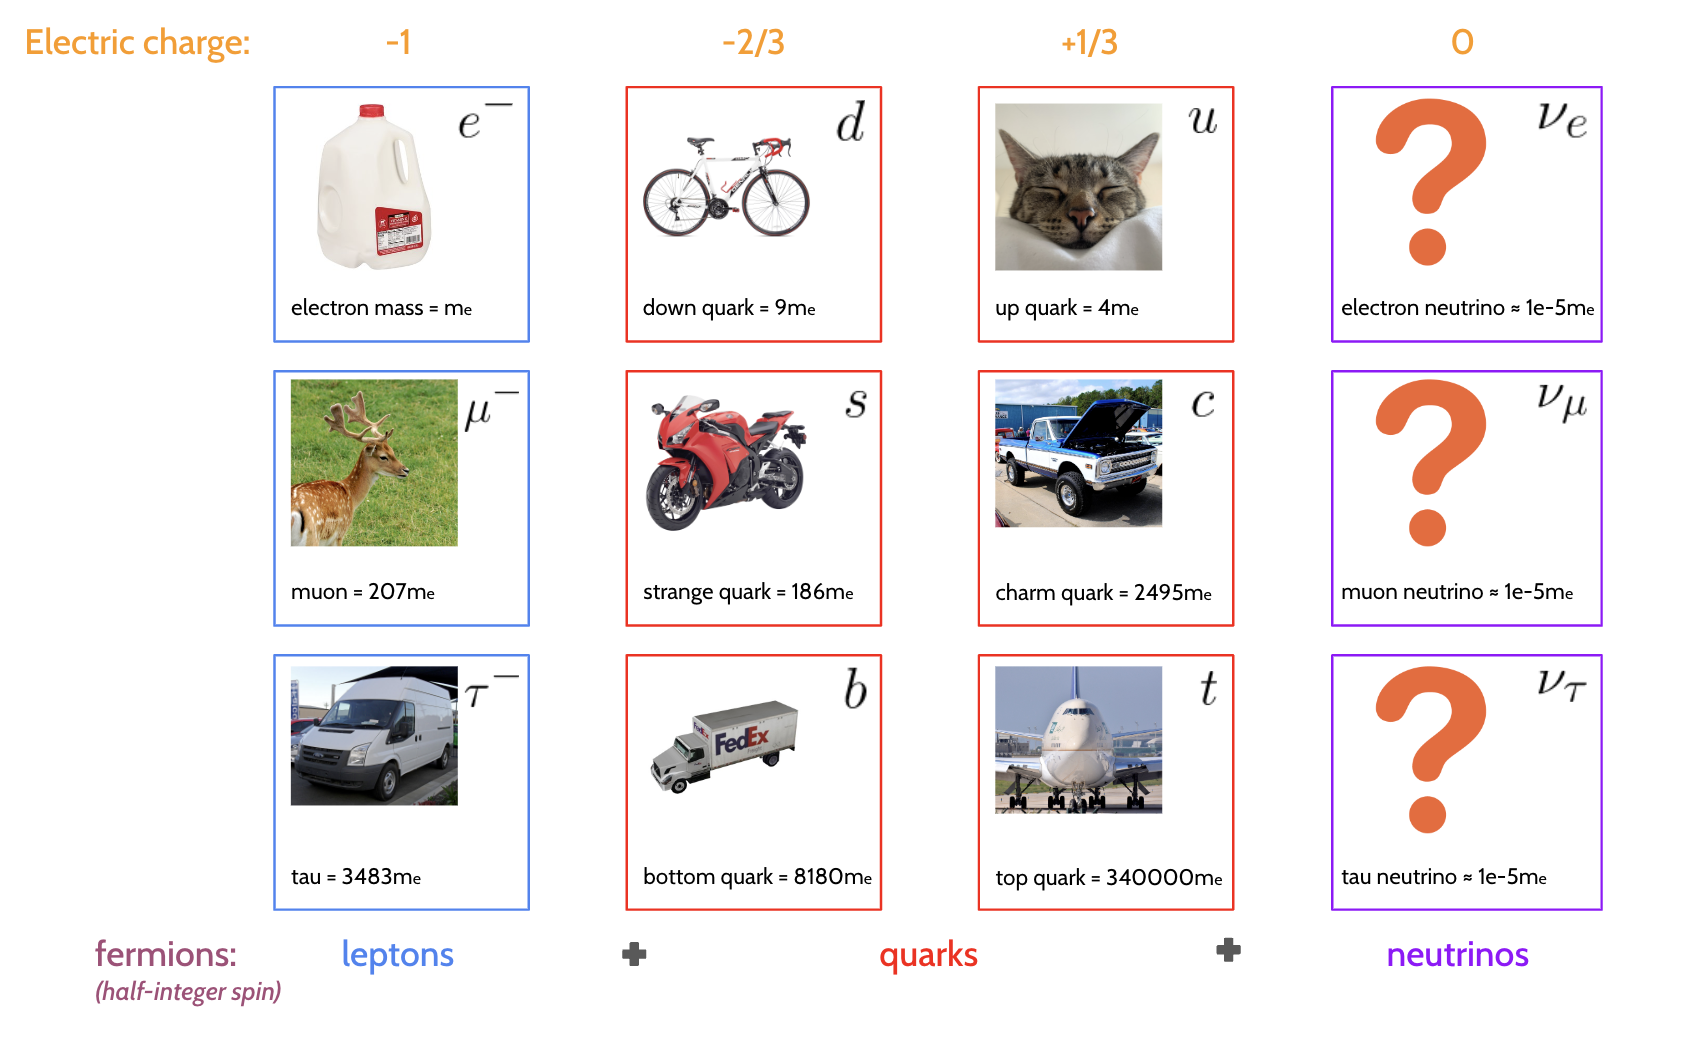
\includegraphics{./images/sm.png}

}

\caption{\label{fig-sm}A cartoon schematic of the Standard Model
fermions. Images are examples of objects that weigh about the same
relative mass to the electron, assuming the electron weighed 1 kg.}

\end{figure}

Particles carry an intrinsic angular momentum, known as \textbf{spin}.
If you want a mental picture, this can be thought of to some degree as
the particles literally spinning in place, but it's of course more a
property of the field than the particles themselves. The main thing to
note about spin is that it's quantized into half-integer amounts
(e.g.~1/2, 1, 1+1/2 etc.), and the sign indicates the direction of that
spin. Importantly, particles with half-integer spin cannot occupy the
same location, which is known as the Fermi exclusion principle. We can
also define the notion of \textbf{handedness}: a (massless) particle is
left-handed if its spin vector and momentum vector are pointing in the
same direction, and right handed if they're pointing opposite
directions.

We come to yet another notion of particles: \textbf{antimatter}. Each
particle in the table above has an antimatter counterpart, denoted
either with a bar over the letter for quarks and neutrinos
(\(\bar{u}, \bar{\nu_\mu}\)) and through flipping the sign of the charge
for leptons (such as the positron \(e^+\)). This is just notation;
antimatter is a flipping of the sign of some of the basic properties of
the particle, namely the electric charge and the handedness. We note
here that whether the neutrino is its own antiparticle is a subject up
for debate; it is unknown if right-handed neutrinos (or left-handed
antineutrinos) exist at all.

\hypertarget{forces}{%
\subsection{Forces}\label{forces}}

When two particles feel a force, it's often said that those particles
undergo the exchange of the relevant particle to that force,
i.e.~there's a \emph{mediator} for every force in the form of a
particle. But in my mind, this leads to weird images of some particles
throwing other particles off one another, which is then somehow meant to
manifest as something like gravity or magnetic attraction, neither of
which seem intuitive\footnote{I would love to give an analogy here like
  waves getting bigger or smaller after exchanging different waves
  between them (since forces and particles are all excitations of
  fields), but I don't have enough grounding in the details to assert if
  it's a good one. Indeed, the ``intuition'' of a field theory is more
  just working through the large number of equations that describe an
  interaction, and then being content enough with your effort that you
  claim to have understanding of how it works. Instead of going down
  this rabbit hole, we'll take the scope-driven decision to leave a good
  reference and move on
  (e.g.~\href{https://www.damtp.cam.ac.uk/user/tong/qft.html}{David
  Tong's QFT lecture notes}).}. Nevertheless, it remains a useful
construct to think about these mediator particles from the perspective
of the underlying mathematics. These particles that mediate forces carry
integer spin, and are called \textbf{bosons} for this reason. Here are
the main examples:

\begin{itemize}
\tightlist
\item
  The \textbf{electromagnetic force} (or hypercharge), carried by the
  \textbf{photon} \(\gamma\)
\item
  The \textbf{weak force}, carried by three particles: the \(W^+\),
  \(W^-\), and \(Z^0\) bosons
\item
  The \textbf{strong force}, carried by the \textbf{gluon} \(g\) (named
  for being the glue that keeps protons together)
\item
  \textbf{Gravity}, which is not described by the Standard Model. In
  theory, one could have a force-carrying particle called the
  \emph{graviton}, but this has no experimental evidence yet.
\end{itemize}

\hypertarget{the-higgs-field}{%
\subsubsection*{The Higgs field}\label{the-higgs-field}}
\addcontentsline{toc}{subsubsection}{The Higgs field}

To top off our description of the Standard Model, we mention the
\textbf{Higgs field}, with a quantum of energy known as the
\textbf{Higgs boson}. The field (and particle) are the only ones in the
Standard Model without any spin, which is what we call a \textbf{scalar
field}. This property leads to a surprising fact: the value of the Higgs
field can be \emph{non-zero in the vacuum}. The reason for this is due
to the shape of the \textbf{potential energy} of the Higgs field, which
can be loosely thought of as how much energy the Higgs field needs to
have to take on a certain value. In the Standard Model, this potential
\(V(\phi)\), where \(\phi\) is the value of the Higgs field, has the
relatively simple form

\begin{equation}\protect\hypertarget{eq-higgs-potential}{}{
V(\phi)=a|\phi|^2+b|\phi|^4~.
}\label{eq-higgs-potential}\end{equation}

The Standard Model predicts the shape of this potential as shown in
Figure~\ref{fig-higgs-potential}, which is only possible with \(a < 0\)
and \(b > 0\). In the absence of anything else, i.e.~in the vacuum, the
Higgs field will sit somewhere at the minima of this potential. But as
shown in Figure~\ref{fig-higgs-potential}, the values of the field in
this valley are non-zero.

\begin{figure}

{\centering 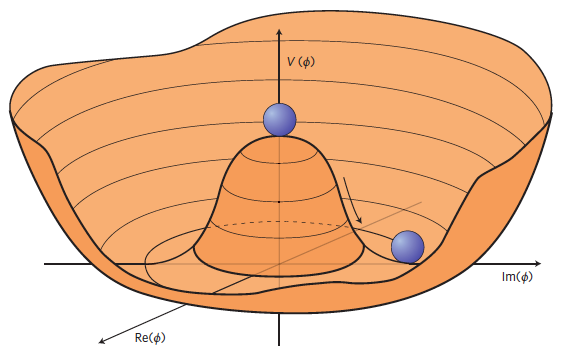
\includegraphics{./images/higgspotential.png}

}

\caption{\label{fig-higgs-potential}An example of the shape of the Higgs
potential predicted by the Standard Model. A cartoon ball is shown to
indicate that the Higgs will settle in one of the low-energy states away
from the origin. Attribution: (Oxford University 2021)}

\end{figure}

A consequence of the Higgs field being ``turned on'' in the vacuum with
some value of energy is that it is responsible for giving
\emph{fundamental particles mass}. Here, I stress the word
``fundamental'' -- the mass of composite particles made of quarks (or
\textbf{hadrons}) is actually due to large fluctuations of the
associated quantum fields, where the Higgs-given masses are a negligible
contribution (the mass of the proton is about 1836\(m_e\), which is
clearly larger than two up quarks and one down quark from
Figure~\ref{fig-sm}). An often-quoted analogy that holds very delicately
is treating the Higgs field as a thick, viscous liquid (think Marmite),
and particles then gain mass as they move through it, with the amount of
resistance depending somehow on the type of particle. This interaction
is technically a fifth force called the Higgs force, but it's not often
quoted as such.

The particle discovered by the ATLAS and CMS experiments at CERN in 2012
is widely believed to represent the Higgs boson as proposed by the
Standard Model (ATLAS-Collaboration 2012). This is largely due to the
mass measured for the Higgs boson being consistent with the Standard
Model prediction of \(m_H \approx 125\) \(\text{GeV}\). For something
fairly up-to-date, a summary of Higgs mass measurements can be found in
Figure~\ref{fig-higgs-mass}. However, it is precisely the fact that the
Higgs is this mass that has left the field of particle physics in a bit
of a muddle. We'll touch on this at the end of the chapter.

\begin{figure}

{\centering 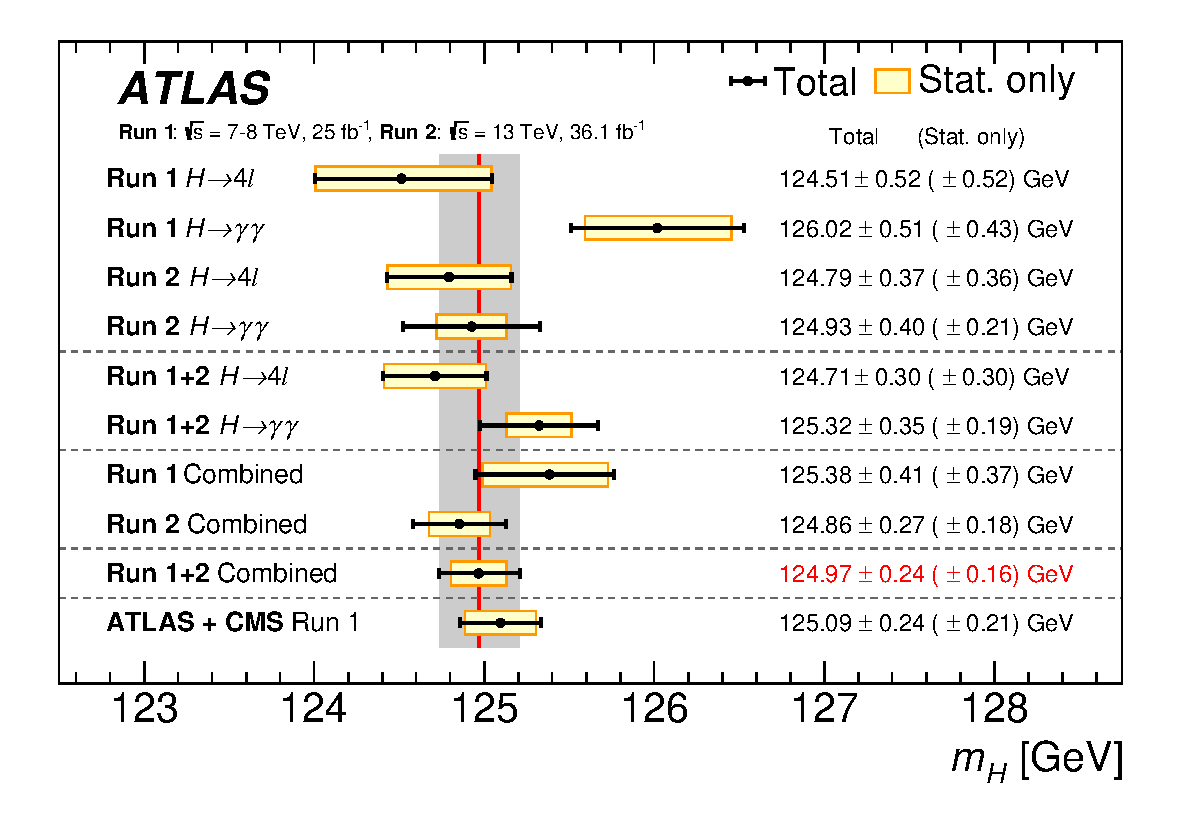
\includegraphics{./images/higgsmass.pdf}

}

\caption{\label{fig-higgs-mass}Summary of the main Higgs boson mass
measurements with their associated errors. Attribution: (ATLAS
Collaboration 2022a)}

\end{figure}

\hypertarget{decays-of-the-higgs-boson}{%
\subsubsection*{Decays of the Higgs
boson}\label{decays-of-the-higgs-boson}}
\addcontentsline{toc}{subsubsection}{Decays of the Higgs boson}

For all this talk of the Higgs boson, it doesn't stop around for long.
It has a lifetime of \(1.6 \times 10^{-22}\) seconds, which is a number
smaller than a second by a factor of around a billion squared. The
result of this is that the Higgs will decay into other particles nearly
instantly within our particle detectors -- we're then left to chase its
shadow. The Higgs can decay into many different particle types,
provided, of course, their total mass does not exceed that of the Higgs
(conservation of energy). However, it is more likely to decay to some
things than others. These different probabilities for particles to decay
into each variety are known as \textbf{branching ratios}, with the
Higgs' most common decay being to two \(b\)-quarks. We can see these
branching ratios as a function of the Higgs mass in
Figure~\ref{fig-higgs-ratios}, where we have a little look either side
of the measured mass from our experiments.

\begin{figure}

{\centering 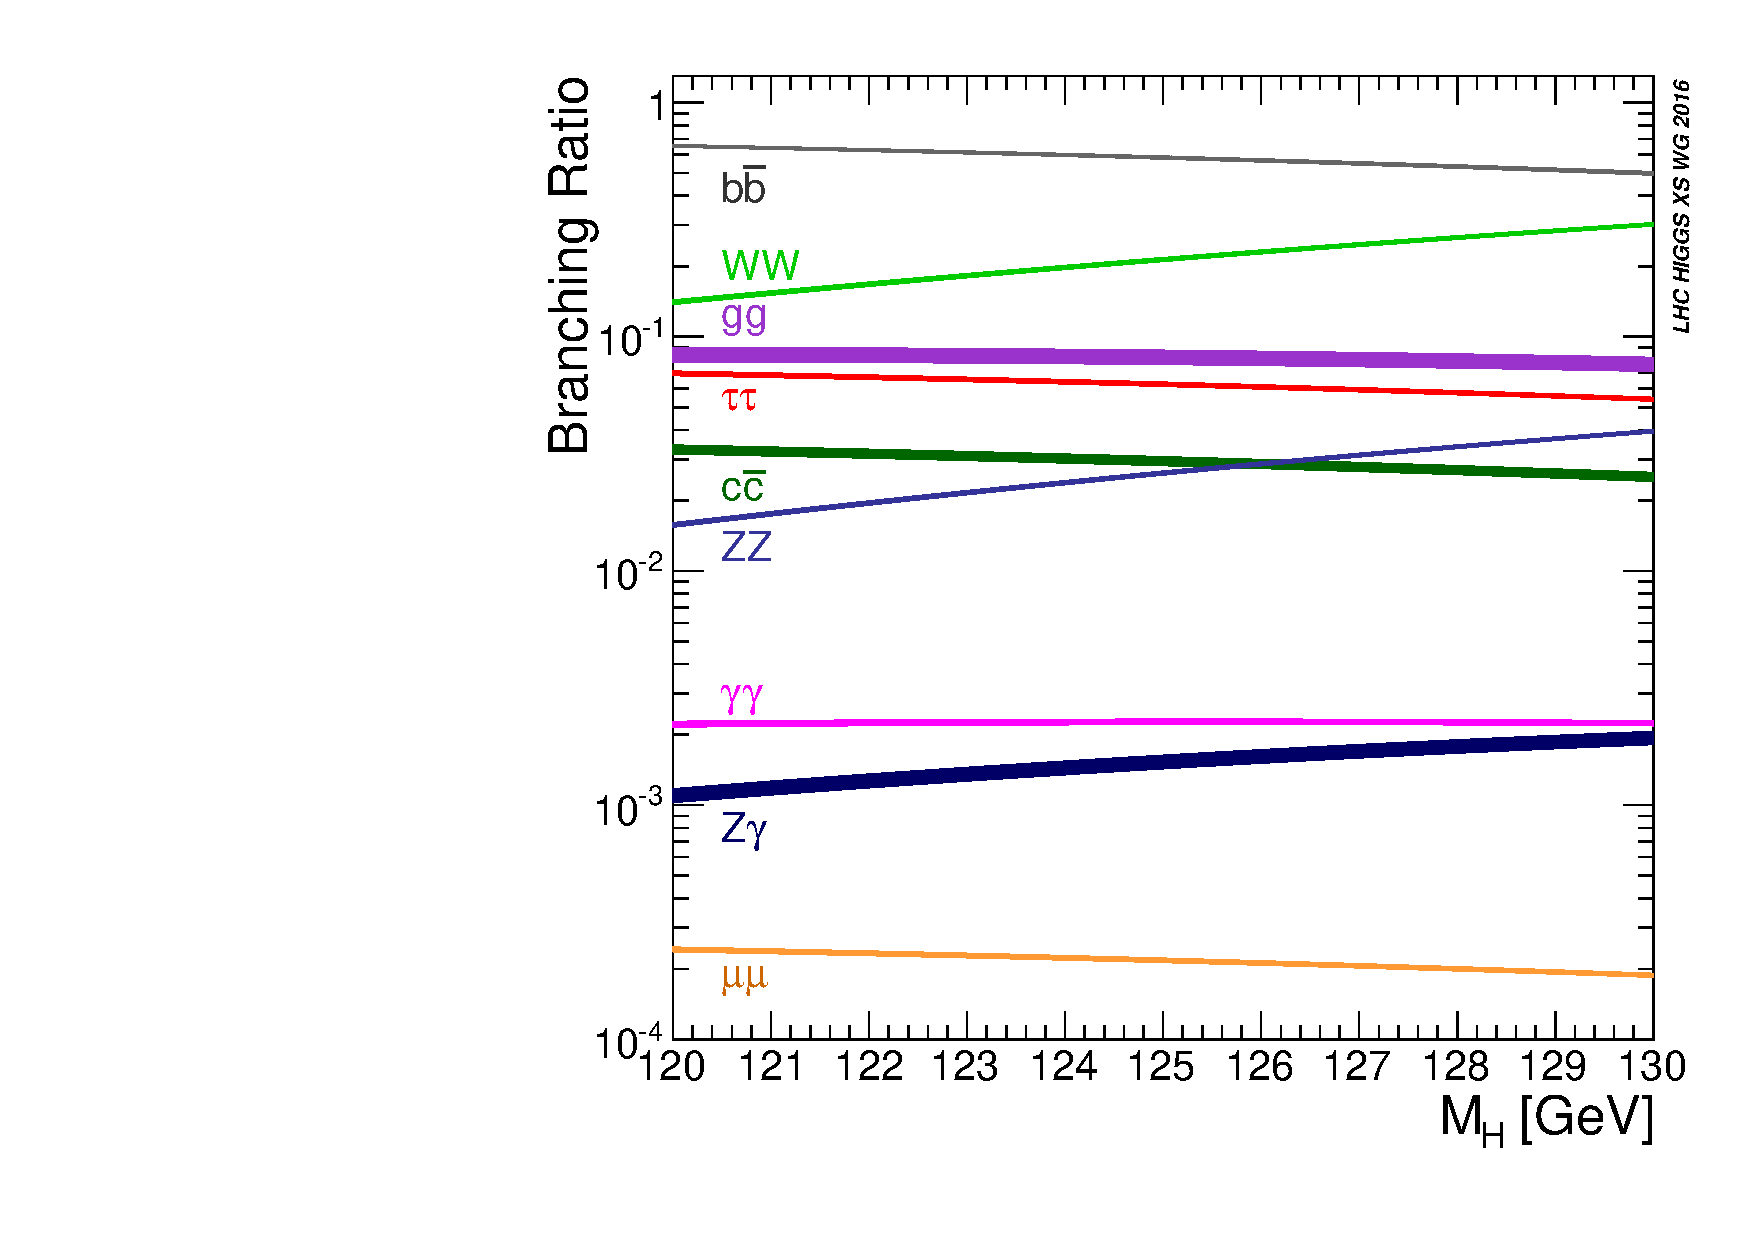
\includegraphics{./images/SMHiggsBR_120-130.pdf}

}

\caption{\label{fig-higgs-ratios}Branching ratios of the Standard Model
Higgs boson to its main decay modes as a function of mass. Attribution:
(CERN 2017)}

\end{figure}

A general note on decays: you'll see decays to two quarks written
sometimes as \(qq\), \(bb\) etc, but any decay to two identical quarks
means one of them is an anti-quark, for reasons of conservation of
charge amongst other things. So \(H\rightarrow bb\) means
\(H\rightarrow b\bar{b}\), just in case I'm not explicit in future.

\hypertarget{properties-of-particles-and-their-colliders}{%
\section{Properties of particles (and their
colliders)}\label{properties-of-particles-and-their-colliders}}

Due to the equivalence of mass and energy (think \(E=mc^2\)), one could
imagine the ability to create things with large mass, if we had enough
energy to do so. That is precisely the idea behind \textbf{particle
colliders}: we give particles a large amount of energy (i.e.~they're
traveling close to the speed of light), and then collide them so that
they interact. These interactions, with sufficient energy, can then lead
to the creation of heavier particles, provided that particle has mass
that's less than the energy at which the particles that produced it
collided. We call this energy the \textbf{center-of-mass energy}, which
is around \(13.6 \,\text{TeV}\) for run 3 of the Large Hadron Collider.
This process of collision is usually done through charged particles such
as protons, because we can accelerate them using electric and magnetic
fields to speeds that can produce energies like this.

How do we detect if we produced the particles we want? We can do this by
analyzing data from the collision; for that, we need to surround areas
of our collider with \textbf{detectors}, which collect all the
by-products that splash out from the center of the collision. These
detectors, along with some input from software, have the ability to
\emph{reconstruct} the tracks that (charged) particles leave in the
detector, from which one can determine properties like the charge from
the way the track curves. Additionally, there are modules that can
measure the energy deposited from particles emerging from the
collisions, which can be placed at different distances to measure
particles with different lifetimes (short-lived particles that decay
quickly won't ever make it past a certain distance before being totally
absorbed by the detector itself).

Given this, we'll go over some of the properties that particles have
while moving, and why they're useful for looking at the validity of
physical theories.

From here, we will use the convention of \textbf{natural units}, which
essentially absorbs constant factors of the speed of light \(c\) and the
Planck constant \(\bar{h}\) into the units chosen. You will then see
quantities quoted in \textbf{electron volts} (\(\text{eV}\)) with
different prefactors as usual for the size (\(\text{GeV}\) = giga
electron volts = \(1\times 10^9\) \(\text{eV}\) etc.). \(1\,\text{eV}\)
is a very small amount of energy indeed (\(1.6 \times 10^{-19}\)
Joules), with the center-of-mass energy of the Large Hadron Collider
being \(13.6\) TeV -- still much less than a sandwich (but I would
support building a sandwich collider; see (Doglioni et al. 2019) for an
attempt of this nature, though physics results may vary).

\hypertarget{kinematics}{%
\subsection{Kinematics}\label{kinematics}}

We start with \textbf{relativistic kinematics}, i.e.~how things move
when they're nearly at the speed of light. Objects like this are best
described by talking about \textbf{spacetime}, which imparts an extra
temporal dimension to the traditional three-vector for position in the
form of a four-vector:

\[
x^\mu = (t, x, y, z) = (x_0, x_1, x_2, x_3)~.
\]

Equivalently, we can drop the index \(\mu\) from upper to lower, and get
the equivalent \(x_\mu = (t, -x, -y, -z) = (x_0, -x_1, -x_2, -x_3)\)
(choice of convention). This allows for the compact notation of dot
products between four-vectors using summation notation:

\begin{equation}\protect\hypertarget{eq-four-vec-prod}{}{
x^\mu y_\mu = y_\mu x^\mu  = x_0y_0 - [x_1y_1 + x_2y_2 + x_3y_3]~.
}\label{eq-four-vec-prod}\end{equation}

This quantity is important, as it can be shown to be
\emph{Lorentz-invariant}, which means the value remains the same even if
we change the reference frame we're in (i.e.~we move in some way
relative to the object). Using the four-vector for position, we can
define a four-momentum:

\[
p^\mu = m \frac{dx^\mu}{d\tau}~,
\]

where \(m\) is the object \textbf{rest mass}, and \(\tau\) is the
\textbf{proper time}, defined by applying the relativistic factor
\(\gamma\) to time as

\[
t = \gamma\tau;~~~ \gamma = \frac{1}{\sqrt{1-v^2}}
\]

for magnitude of the object's three-velocity \(v = |\mathbf{v}|\). This
leads to an equivalent notation of

\[
p^\mu = (E, \mathbf{p}); ~~~ E=\gamma m,~\mathbf{p}=\gamma m \mathbf{v}~.
\]

Using Equation~\ref{eq-four-vec-prod}, we can take the dot product of
\(p^\mu\) with itself:

\begin{equation}\protect\hypertarget{eq-mom-dot}{}{
p^2 = p^\mu p_\mu = E^2 - |\mathbf{p}|^2~.
}\label{eq-mom-dot}\end{equation}

We can exploit the fact that \(p^2\) is invariant to its reference frame
and examine one case in particular: a stationary body with 0 velocity
but some mass will have a non-zero four-momentum \(p^\mu = (m, 0)\).
Then, we have \(p^2 = m^2\), which we can set equal to
Equation~\ref{eq-mom-dot} that holds generally:

\begin{equation}\protect\hypertarget{eq-invariant-mass}{}{
\Rightarrow E^2 - |\mathbf{p}|^2 = m^2~,
}\label{eq-invariant-mass}\end{equation}

which is called the \textbf{energy-momentum relation}, and leads to the
left-hand side being known as the \textbf{invariant mass} \(s\), since
it recovers the rest mass of a body in that body's rest frame. Of
course, \(\sqrt{s}\) is then the actual rest mass in this case, which is
why we write \(\sqrt{s} = 13.6 \, \text{TeV}\) as the center-of-mass
energy for the LHC.

For multiple particles, Equation~\ref{eq-invariant-mass} then gives rise
to the concept of the invariant mass of a system of bodies with
four-momenta \(p_1, p_2, ...\) -- their total momenta is \(\sum_i p_i\),
and the total invariant mass is then

\begin{equation}\protect\hypertarget{eq-invariant-mass-system}{}{
s_{1,2,...} = \left(\sum_i p_i\right)^2 ~,
}\label{eq-invariant-mass-system}\end{equation}

which will involve terms in the energies and three-momenta of the
different particles as per Equation~\ref{eq-invariant-mass}. This
quantity will be particularly important when we come to the search for a
new particle in the latter stages of the thesis, because it allows us to
detect \textbf{resonances}, which are intermediate particles that can
produce a different final state. As an example, the Higgs boson can
decay to four leptons via other vector bosons as per
Figure~\ref{fig-higgs-ratios} (e.g.~two \(Z\) bosons can each decay into
two leptons), meaning the Higgs can then be found in the invariant mass
of this four-lepton system, \(m_{4l}\). We can see this in
Figure~\ref{fig-higgs-m4l}, where there's a peak at the Higgs mass of
\(m_H \approx 125\) \(\text{GeV}\), since the invariant mass of the
initial state (a Higgs boson with \(E^2 - |\mathbf{p}|^2 = m_H^2\)) is
equal to that of the final state (four leptons) by energy/momentum
conservation.

\begin{figure}

{\centering 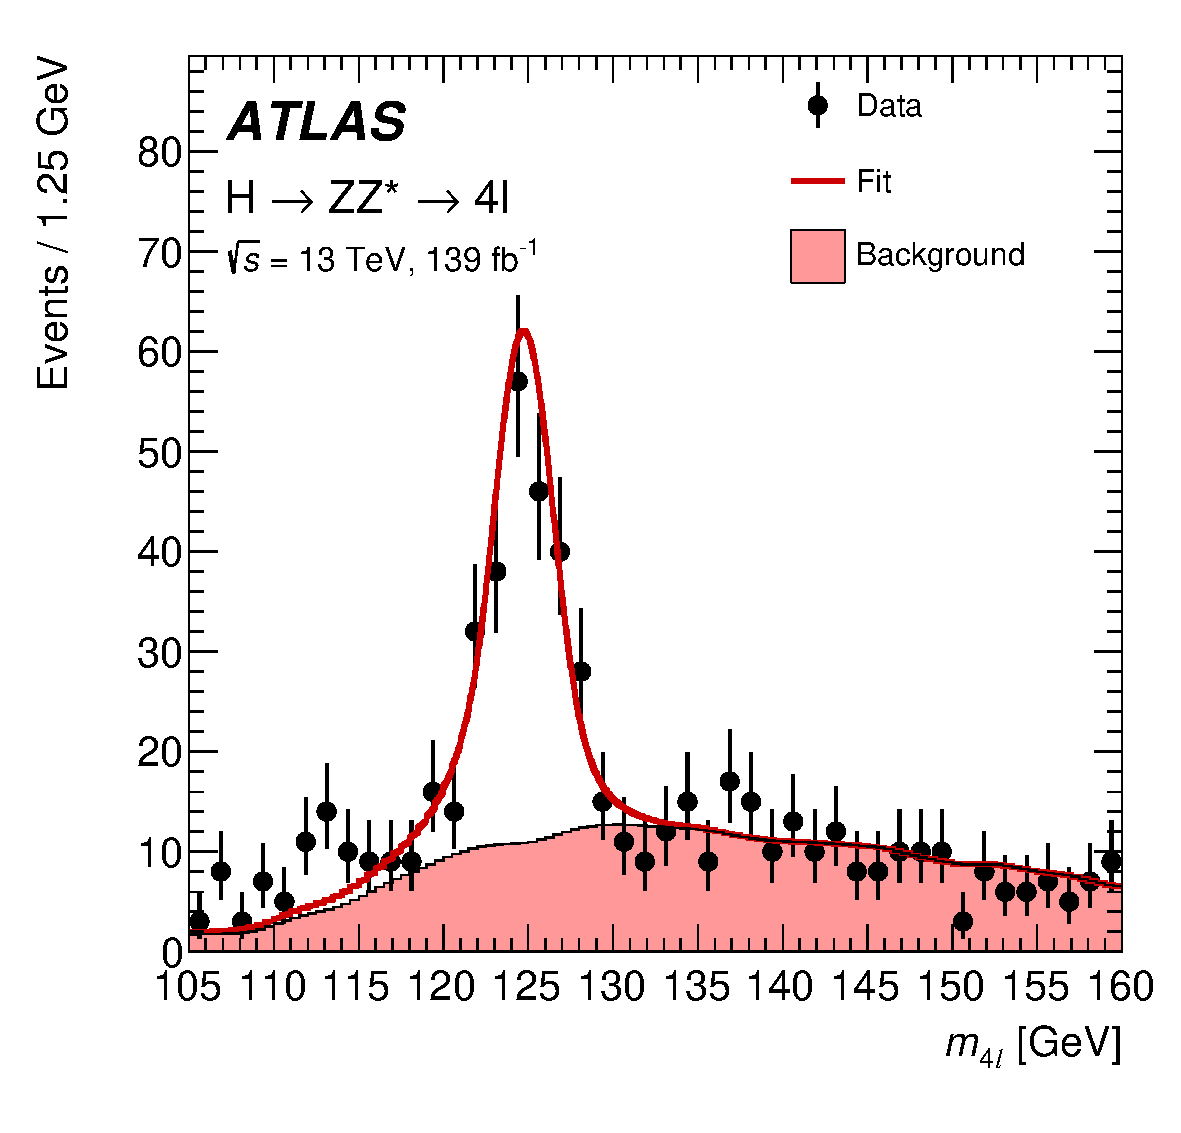
\includegraphics{./images/higgsm4l.pdf}

}

\caption{\label{fig-higgs-m4l}An example plot of the four-lepton
invariant mass, taken from a recent Higgs boson mass measurement in this
final state. Attribution: (ATLAS Collaboration 2022b)}

\end{figure}

\hypertarget{quantifying-collisions}{%
\subsection{Quantifying collisions}\label{quantifying-collisions}}

An interaction between colliding particles (that usually produce some
measurable detector output) is called a \textbf{scattering event}, or
more simply just an \textbf{event}. To cause an event then, indeed,
particles must collide. What's the chances of that happening? If we were
instead talking about two tennis balls colliding, there would be an idea
of a cross-sectional area influencing this, whereby if the tennis ball
were to enter that region, collision of some variety would occur due to
the balls being close enough, with the rate of this occurring being
related to the size of that area. A similar quantity exists for
particles colliding, which we call the \textbf{scattering cross-section}
\(\sigma\) (or just cross-section). The details on how one calculates a
cross-section are more complicated for particles, but quantum field
theory has exact rules for this that involve quantities called
scattering amplitudes, and also performing an integral over the space of
momenta of the initial state particles. I omit the details as they are
beyond the scope of my work -- see e.g.~section 2.7 of (Buckley, White,
and White 2021) for more. We will go as far to state this: given a
number of scattering events \(N\) (every interaction between some set of
colliding particles), the rate of these events occurring is directly
proportional to the cross-section, i.e.

\begin{equation}\protect\hypertarget{eq-cross-section}{}{
\frac{dN}{dt} \propto \sigma~~~\Rightarrow \frac{dN}{dt} = \mathcal{L}(t) \sigma~,
}\label{eq-cross-section}\end{equation}

where we've denoted the constant of proportionality as the
\textbf{luminosity} \(\mathcal{L}(t)\), which generally can be a
function of anything to do with the structure of the colliding objects
(e.g.~beams of particles) at some time \(t\). We can see that increasing
\(\mathcal{L}(t)\) increases the event rate; this leads to the analogy
of beams of colliding particles being ``brigher'' with higher
luminosity, hence the name.

We can also state that the overall cross-section of some collision is
equal to the sum over the cross-sections for mutually exclusive physics
processes \(i\) (as to not double count): \(\sigma = \sum_i \sigma_i\),
and we have individual equations

\[
\frac{dN_i}{dt} = \mathcal{L}(t) \sigma_i~.
\]

The take-home from this is that for any physics process, the event rate
in a collision will be a function of a term that dictates the underlying
physics (\(\sigma_i\)) and a term that is influenced by beam structure
(\(\mathcal{L}(t)\)). Moreover, we can define an overall
\textbf{integrated luminosity} \(L\) as a metric of cumulative beam
``brightness'' up to some time \(T\) by integrating
Equation~\ref{eq-cross-section}:

\[
L = \int_0^T \mathcal{L}(t) dt = N/\sigma~.
\]

The cross-section has units of area (m\(^2\)), and is usually quoted in
\emph{barns}, where 1 b = \(10^{-28}\) m\(^2\). Since \(N\) is unitless,
the luminosity then has units of inverse barns, which are usually quoted
at the femto scale (fb\(^{-1}\)).

\hypertarget{particle-detectors}{%
\section{Particle detectors}\label{particle-detectors}}

We'll say a few words on the detectors that are used to measure these
particle collisions, with a focus on the ATLAS detector at CERN ATLAS
Collaboration (2008).

ATLAS is the name for both the detector that wraps around part of the
beam pipe at the Large Hadron Collider, the experiment that it conducts,
and for the collaboration of people that work on building the detector
and analyzing the resulting data. The detector itself is split up into
four concentric parts: the \textbf{inner tracking detector},
\textbf{electromagnetic calorimeter}, \textbf{hadronic calorimeter}, and
the \textbf{muon detector}, which are in the toy schematic shown in
Figure~\ref{fig-detector}. Each part has a different job, which is
summarized in the following paragraphs.

\begin{figure}

{\centering 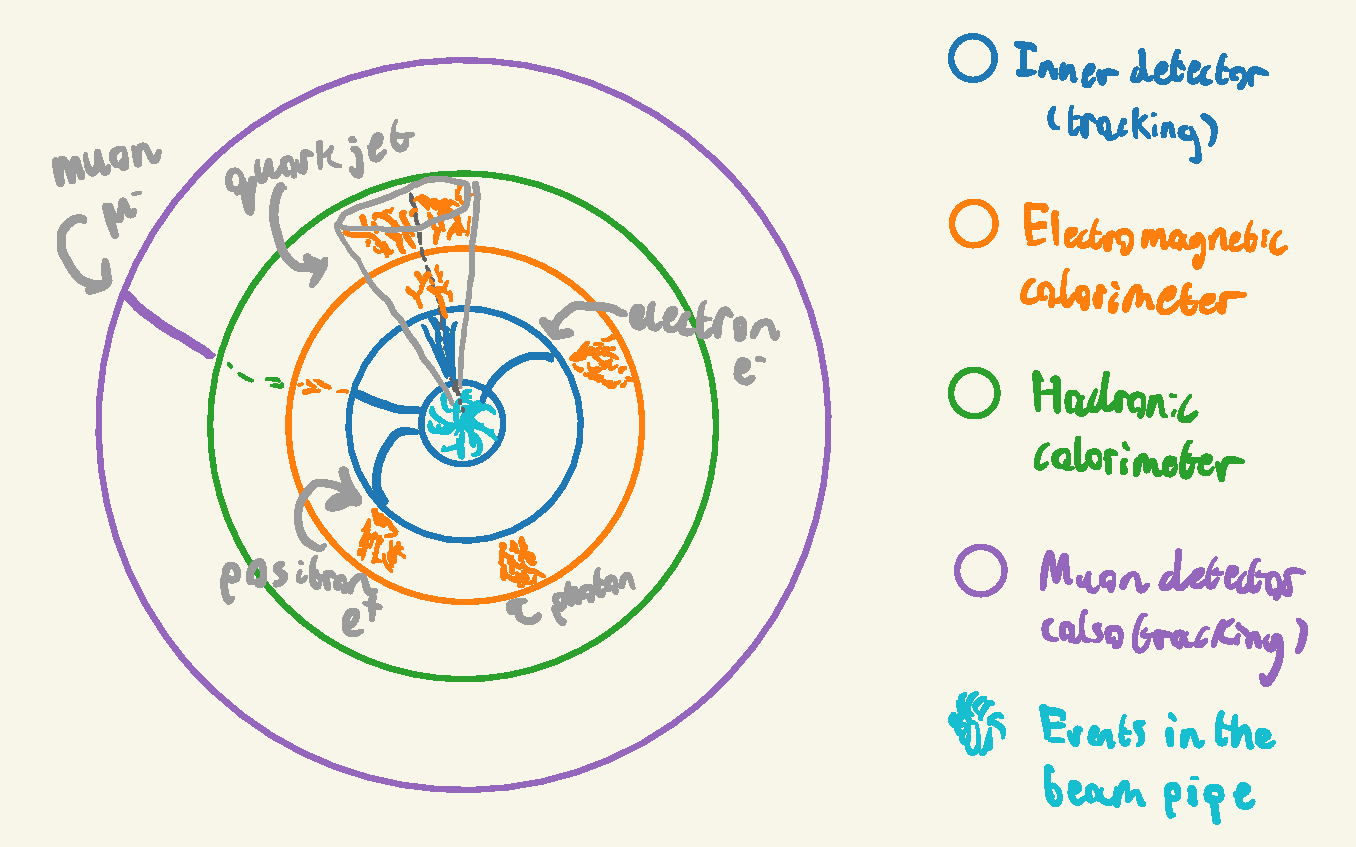
\includegraphics{./images/detector-schematic.pdf}

}

\caption{\label{fig-detector}A toy schematic for the transverse
cross-section of an imagined particle detector for collisions of two
beams. The signatures different types of particles would leave are
depicted within the detector.}

\end{figure}

The inner detector tracks charged particles that leave \emph{hits};
these come from things like ionization of a gas as the particle moves
through, and having charged wires that collect the free electrons from
the ionization. By trying to intelligently draw a line through these
hits, e.g.~by fitting a functional form, we can reconstruct the shape of
the track. To measure the properties of charged particles emerging from
collisions like the charge and momentum, we can look at the curvature of
the track. To bend particles in the detector so that they have
curvature, we need to apply a magnetic field that causes the particles
to move in circular motion in the transverse plane (i.e.~perpendicular
to the direction of the beam). ATLAS does this by surrounding it's inner
detector with a solenoid magnet (and toroidal magnets on the barrel and
endcaps).

You'll have noticed there are two calorimeters -- this is because
electrons and photons penetrate material much less deep than hadrons, so
they're separated into two different parts. Calorimeters in general
measure \emph{energy deposits} by having the particles collide with some
dense material, which causes energy loss in some way, and then
interlacing that material with something that can collect information on
the energy of the resulting products from traveling through the dense
medium. The \emph{electromagnetic calorimeter} is responsible for doing
this for electrons and photons, where they undergo energy loss by
scattering and Bremsstrahlung radiation. It's worth noting that quarks
are never observed standalone in a detector. Instead, they rapidly decay
into sprays of collimated \textbf{hadrons} (particles containing quarks)
by the process of hadronization. We refer to these structures as
particle \textbf{jets}. The \emph{hadronic calorimeter} exists to detect
hadrons from these particle jets, where their main source of energy loss
is scattering processes with the calorimeter material.

The final part is the muon detector, which sits external to all other
detectors, and is also a tracking detector like the inner detector. The
muon passes through the inner detector and calorimeters, but typically
will not lose much energy like other particles might from scattering or
Bremsstrahlung. That means that if we have a tracking detector far from
the beam pipe, it's likely that anything it picks up will be a muon.

\hypertarget{kinematics-again}{%
\subsection{Kinematics, again}\label{kinematics-again}}

Using the information the detectors give us, we can summarize an event
by the properties of the objects that the detector picked up as a
result. We can think of an event as a list of particles with
four-momenta, and one additional entry that has the missing
four-momentum compared to the total inital proton four-momenta, which
could include particles invisible to the detector like neutrinos. These
four-momenta are typically transformed to a different set of coordinates
that better fit with describing the geometry of the detector itself.

If we denote the beam axis as the \(z\) direction, the \(x\)-\(y\) plane
is known as the \textbf{transverse plane}, which groups the
three-momentum of a particle into \(\mathbf{p} = (\mathbf{p}_T, p_z)\).
One will often hear about the magnitude \(p_T = |\mathbf{p}_T|\) being a
quantity of interest, which is due to the fact that objects with high
\(p_T\) will likely be much easier to reconstruct and measure precisely,
since they are not mixed up with all of the colliding proton beam debris
in the \(z\)-direction. For this reason, we're actually not able to
measure \(p_z\) very well, and instead look to variables that are
\emph{invariant} to changes in velocity in the \(z\) direction. One
example of a quantity like this is the \textbf{rapidity}, defined as

\[
y = \frac{1}{2}\ln{\left(\frac{E+p_z}{E-p_z}\right)}~,
\]

which measures how ``forward'' (close to the +ve \(z\) axis) or
``backward'' (close to the -ve \(z\) axis) a particle lies. \(y\) = 0
corresponds to no \(z\) component of the momentum, and \(\pm \infty\)
means the momentum is aligned with the +ve and -ve \(z\) direction
respectively. Particle physicists often use the \textbf{pseudorapidity},
defined as

\[
\eta = -\ln{\left(\tan{\frac{\theta}{2}}\right)}~,
\]

which is equal to the rapidity for particles with energy \(E\) much
higher than their mass \(m\). It's preferred since the polar angle
\(\theta\) between \(z\) and the transverse plane is much easier to
determine than \(p_z\), for instance. We can thus fully specify a
particle's position in the detector with the (pseudo)rapidity and the
azimuthal angle \(\phi\) between the \(x\) and \(y\) directions.

\hypertarget{simulators}{%
\section{Simulators}\label{simulators}}

We are not able to perform our data analysis on collisions where we
\emph{know for sure} what produced them. If we could access this
information, that would allow us to do many practice runs where we tune
things to give us the best chance to discover the signal, if it was
actually there. To this end, countless generations of particle
physicists have worked on building robust \textbf{simulators} that can
produce many Monte Carlo events (read: randomly sampled events from
physics distributions). They work by calculating the different terms in
an expansion as set out by quantum field theory responsible for the
rates of physics processes, known as \emph{perturbative field theory},
to a specified order in the expansion. This is what is referred to by
phrases like \emph{leading order} (LO) and next-to-leading order (NLO)
-- it's the choice of terms you include in the perturbation calculation,
which corresponds to choosing to include the different ways to produce
that given final state you want to produce.

After simulating the physics processes themselves, we're not quite ready
to jump in and optimize our analysis code, because we're not looking at
something that mirrors what we'd expect from our detector. As an
example, it's likely that our detector is only able to measure particle
momenta up to a certain \emph{resolution}, but we have access to the
true values with no uncertainty. To change this, we can apply a layer of
functions that attempt to \emph{smear} the output, e.g.~by sampling
momentum from a normal distribution centered around the true value
instead of using the true value directly, which should mimic the fact
that we're inherently limited in the way we can measure these quantities
in real life. Moreover, we won't be encountering the values of momentum
-- we'll be getting electrical signals from a wire! We need to then do
the additional step of \textbf{digitization}, which turns the physics
quantities into things we'd expect from a detector, such as track hits
and energy deposits.

Once we've done all that, we're free to then attempt to
\textbf{reconstruct} the events just like we would for a regular
detector (essentially building up particle four-momenta from track
information), which allows us to make sure we don't do any better in
getting the physics information than we would be able to in actuality.
We can then use this information as the input for our physics analysis,
and begin to optimize. The only difference is that there's a bias
between the simulation and real data we may struggle to account for, but
we trade off by having a label on each event that tells us which physics
process it came from (i.e.~signal or background). We can see this whole
process depicted in Figure~\ref{fig-simulator}.

\begin{figure}

{\centering 

\begin{figure}[H]

{\centering 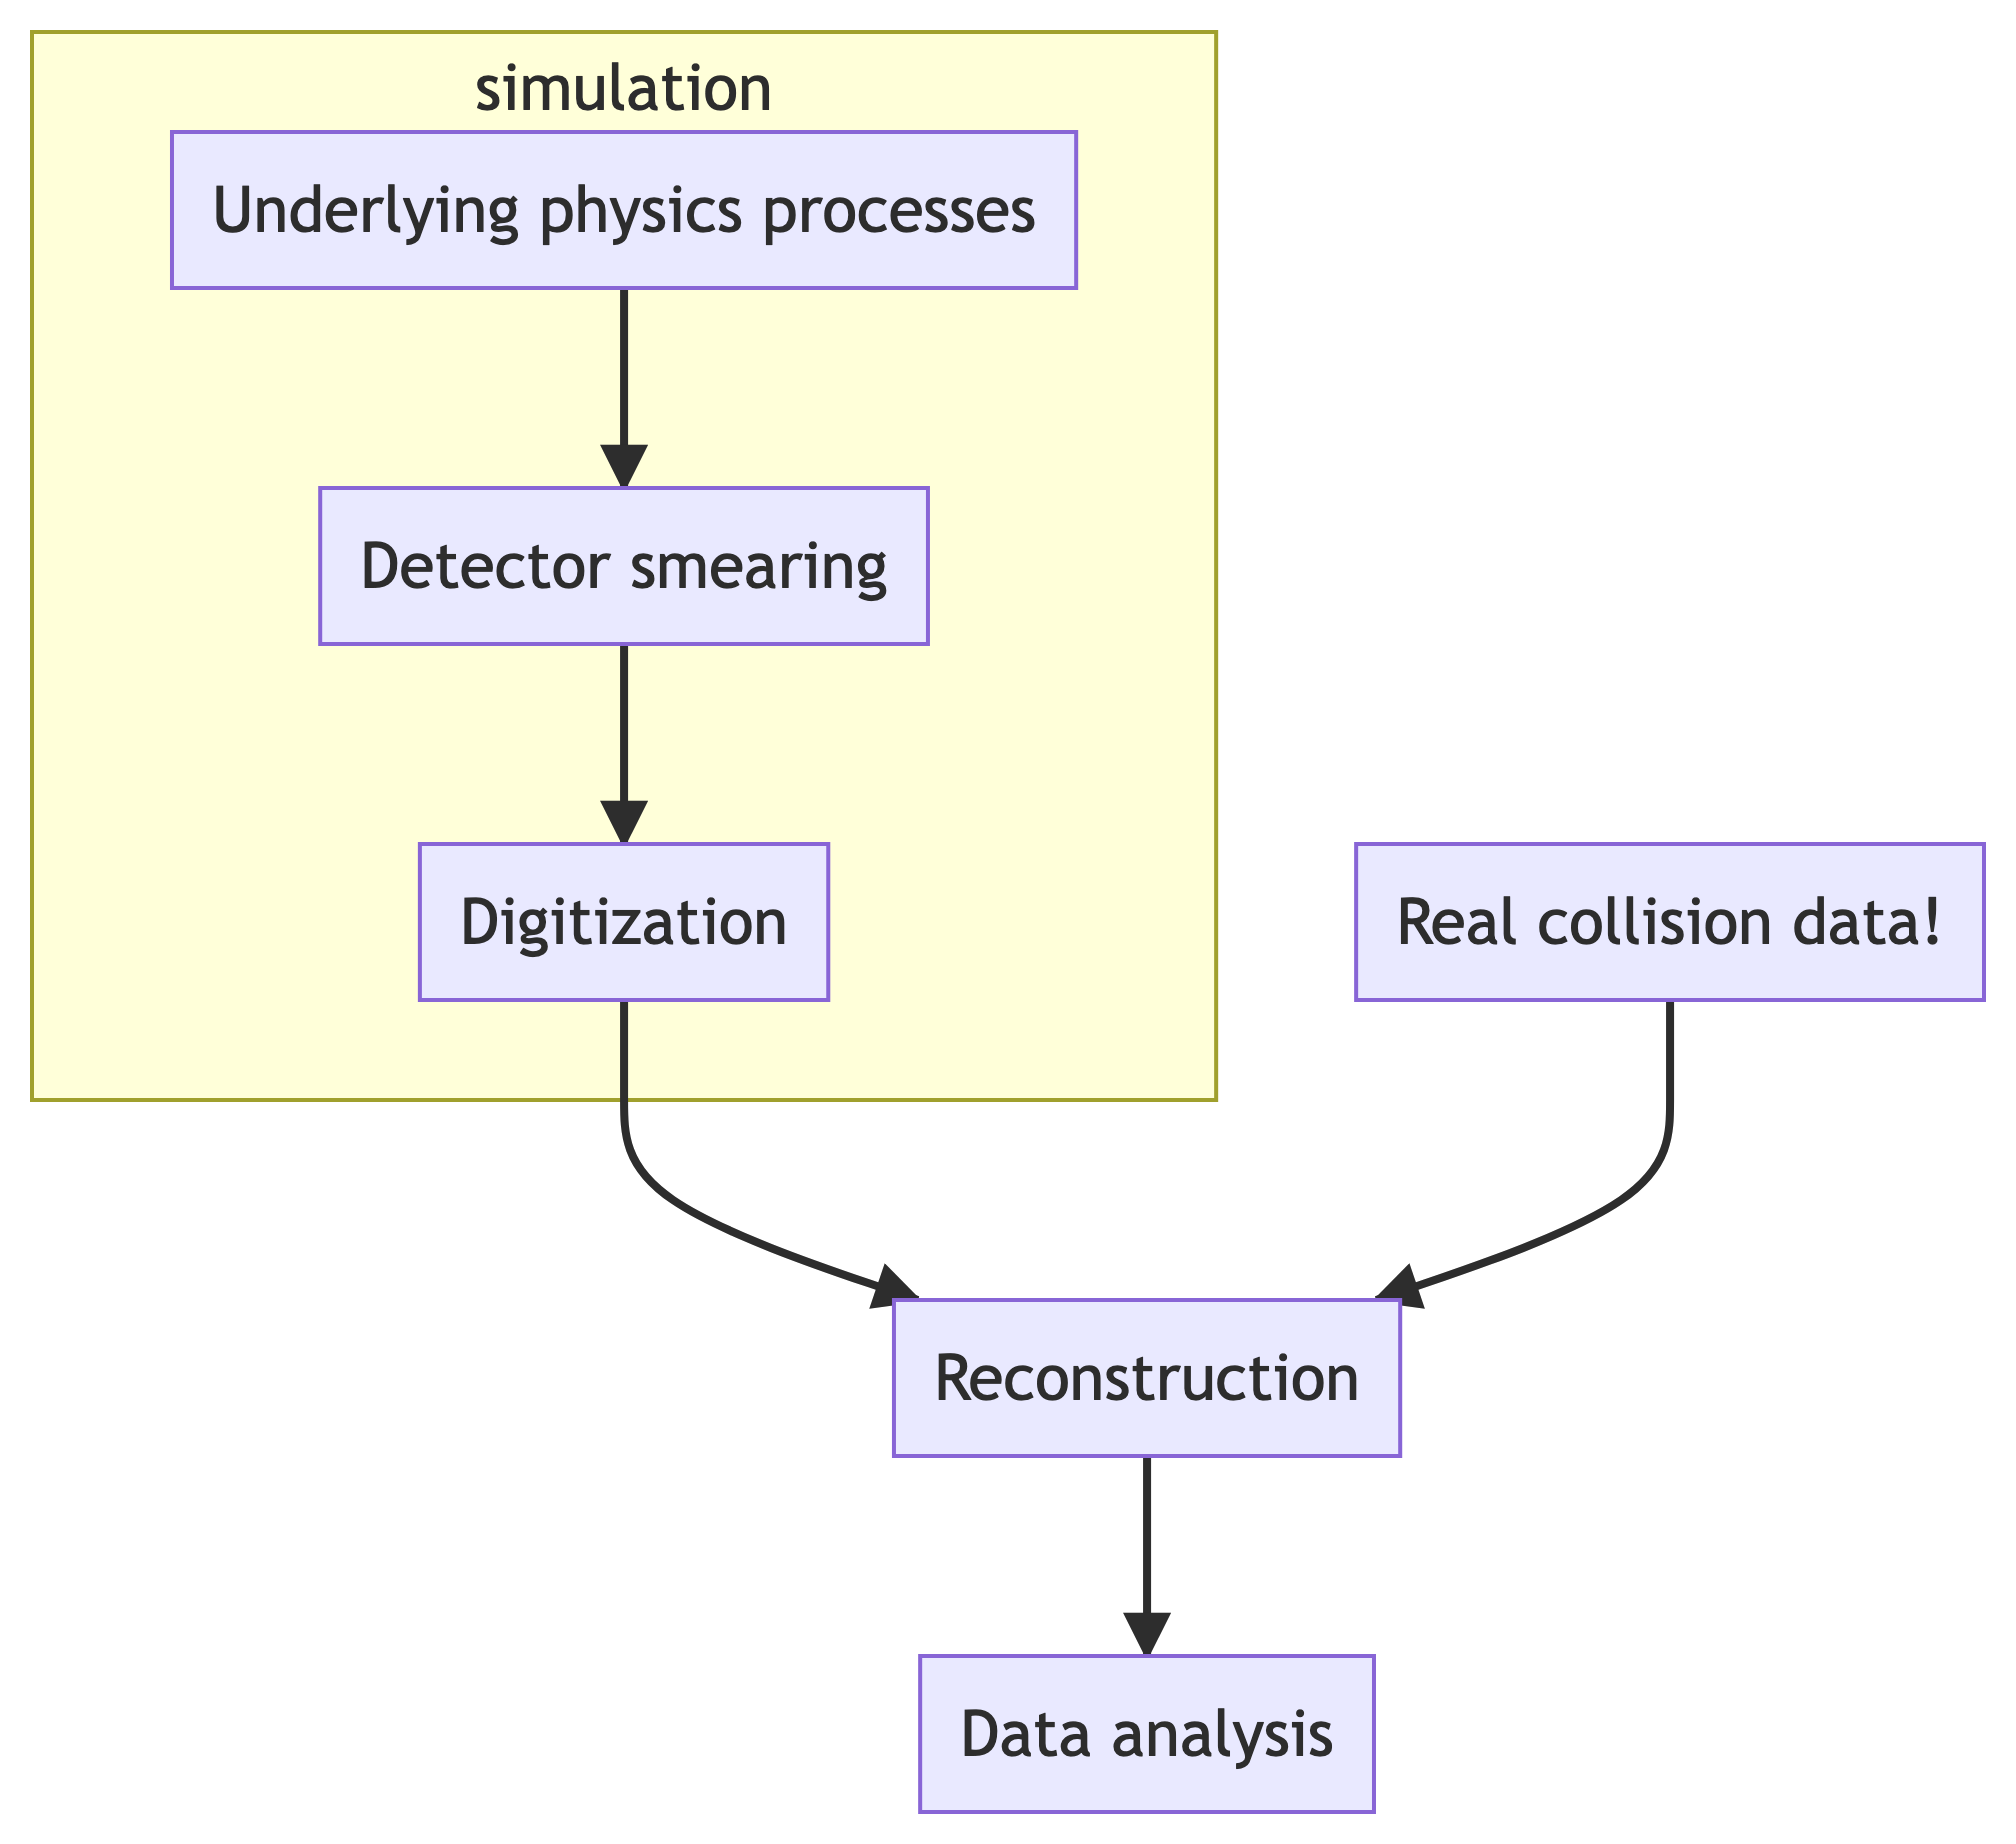
\includegraphics[width=5.5in,height=3.5in]{./physics_files/figure-latex/mermaid-figure-1.png}

}

\end{figure}

}

\caption{\label{fig-simulator}A summary of the different workflow steps
that are taken when simulating particle physics processes, including
mirroring detector effects.}

\end{figure}

\hypertarget{sec-bsm}{%
\section{Issues with the Standard Model, and what may lie
beyond}\label{sec-bsm}}

Here we touch on a few of the cracks in the Standard Model, and some
proposed resolutions. We'll only explore enough to get an idea that it's
certainly worth searching for these solutions in some way!

\hypertarget{the-hierarchy-problem}{%
\subsection{The hierarchy ``problem''}\label{the-hierarchy-problem}}

A property unique to the Higgs boson is that its measured mass is very
sensitive to physics at higher energy scales (read: new particles with
higher masses than discussed here), so the fact that the Higgs is fairly
light at \(125\,\text{GeV}\) is a strong constraint on the scale of new
physics that we're likely to see. Let's explore a little why this is.

Now, in a bit of an aside, quantum field theories are able to work well
due to a process called \textbf{renormalization}, which essentially
amounts to subtracting away infinite quantities that can arise in
calculations involving fields. A consequence of this is that all
parameters of a quantum field theory are inherently linked to some
energy scale (or equivalently distance scale) at which we admit our
ignorance, i.e.~there's an energy \emph{cutoff} at which we say our
theory no longer applies at energies higher than this. We term that
cutoff \(\Lambda_{\text{UV}}\), One surprising thing about the choice of
\(\Lambda_{\text{UV}}\) is that it actually impacts the value of the
Higgs mass! This is because similar to hadrons, the Higgs boson gains
its own mass in part due to the quantum fluctuations of many different
fields, with \(\Lambda_{\text{UV}}\) controlling the scale of these
fluctuations. These are colloquially termed as quantum ``corrections''
to the value of the mass. So when we measure \(m_H\), what's actually
beneath the curtain? It turns out that \(m_H\) is then actually made up
of two parts:

\[
m_H^2 \approx\left|a+\mathcal{O}\left(\Lambda_{\mathrm{UV}}^2\right)\right| \approx 125 \,\text{GeV}~,
\]

where the parameter \(a\) is part of the formula for the Higgs potential
in Equation~\ref{eq-higgs-potential}. This \(a\) parameter, which is
usually referred to as the \emph{bare mass} (i.e.~what would be the mass
in the absence of corrections), is that it has to be large and negative
if \(\Lambda_{\mathrm{UV}}\) is of any reasonable size in order to
cancel out their values enough to get \(125\,\text{GeV}\).

This isn't necessarily a problem, per se, but it's quite the coincidence
if true. To be as kind as possible to us, we can say Standard Model is
no longer valid just above the current energy scale of the LHC
(\(13600 \,\text{GeV}\)), which would make the parameter \(a\) be of a
similar size such that their sum results in \(125\,\text{GeV}\). This
would mean we'd see some new theory come into play around the
\(\text{TeV}\) scale, which we haven't found evidence for. Of course, to
see \emph{pretty much no signs} that there's new physics at this energy
scale, we'd probably hedge our bets that it holds a bit further out than
this, which would lead to numbers much larger (hundreds of thousands)
having to cancel out precisely to \(125\,\text{GeV}\). Again, this isn't
necessarily an issue -- nature could just be very fine-tuned. But this
is a source of unease for many theoretical physicists, and it remains an
open ``problem'' to find out why this is the case.

\hypertarget{gravity}{%
\subsection{Gravity}\label{gravity}}

It is unfortunate that such a well-tested theory does not adequately
describe gravity, which, at the time of writing, seems to still be doing
its thing. Moreover, Einstein's theory of General Relativity, which
describes gravity, doesn't seem to fit well with all this particle talk,
but it too is a very well-tested theory. This is one of many frustrating
things about having the Standard Model triumph experimentally: we
\emph{know} it's not good enough alone\footnote{I've heard water cooler
  talk about particle physicists even being upset at the Higgs discovery
  for this very reason -- a nail in the coffin for many other theories.},
and it somehow has to interplay with another very important theory,
despite these puzzle pieces having wildly serrated edges. So yeah, we're
not too happy about this.

\hypertarget{other-things}{%
\subsection{Other things}\label{other-things}}

More problems we don't have an answer to include:

\begin{itemize}
\tightlist
\item
  Why do we live in a matter dominated universe instead of antimatter?
\item
  Do the forces of nature unify at a certain energy scale?
\item
  What's the deal with dark matter?
\item
  \ldots and many more!
\end{itemize}

All of these questions have potential answers involving both new physics
theories and verifiable experimental consequences (which makes them
well-posed theories). The agenda of the LHC and many other particle
physics experiments is then to probe them however we can, with the tools
available to us.

\hypertarget{going-beyond-the-standard-model}{%
\subsection{Going beyond the Standard
Model}\label{going-beyond-the-standard-model}}

Just to mention one, the most commonly touted theory that has been
investigated in recent years is \emph{supersymmetry}, which makes it
such that every particle proposed in Figure~\ref{fig-sm} has a
supersymmetric partner at some higher energy scale\footnote{These
  particles have super cute names like sleptons, squarks,
  gluinos\ldots{} I highly recommend reading the Wikipedia page.}.
Importantly, these additions help to stabilize the mass of the Higgs
boson in the hierarchy problem, and also conveniently helps with
unification of forces. It's actually all quite neat, but has the large
drawback of a total lack of evidence for its existence.

There are many more theories of this nature, including many exotic new
particles and ideas, but none seem to have poked their head out at any
of our experiments as of yet. That's why it remains paramount to both
look for these new hypothesized particles and also precisely measure
things that the Standard Model predicts, which may act as a calling card
for a new theory we have yet to discover.

\hypertarget{probability-and-statistics-in-theory}{%
\chapter{Probability and Statistics, in
theory}\label{probability-and-statistics-in-theory}}

It must be said that I have no desire to subject you, the reader, to the
same philosophical torment that I have undergone in my pursuit of
clarity of this topic, which I could not even claim to have reached.
Moreover, given that this is an \emph{experimental} physics thesis, it
is exceedingly likely that you are a pragmatist, and wish to move
swiftly on to the sections that may be useful to your life. Nonetheless,
I'd like you to allow me the courtesy of proposing that there may in
fact be something truly useful in revisiting these foundations, if only
to reaffirm their non-utility.

For this section, my most heavily used and recommended resource is
(Cousins 2018), which I heard Bob himself refer to as his ``life's
work''. Do give it a read -- so many useful gems by someone who took a
lot of time to build bridges between science and statistics!

\hypertarget{probability-distributions-and-likelihood}{%
\section{Probability, distributions, and
likelihood}\label{probability-distributions-and-likelihood}}

Both the pre-amble to and the beginning of my PhD studies were decorated
with thoughts on the nature of probability. At the time, I had just come
out of a Masters degree project that involved the application of
\emph{nested sampling} (Skilling (2006)) to infer the momenta of invisible
neutrinos. This technique was invented by John Skilling, a prolific
figure in the realm of Bayesian statistics, if only for his advocation
thereof (if you're planning to be indisposed for a time, you may find
Skilling (2008) of interest as reading material, but do make sure to
dilute it with things like Senn (2011) and Mayo (2018)). This started me
down a rabbit hole on the much-contended topic of the definition of
probability. It turned out the topic was vast, with arguments both
mathematical and philosophical dating back many hundreds of years, many
of which are still alive in the present day. Of this, I was particularly
surprised --- my undergraduate courses had spent a mere ten minutes or
so on the subject, and I thought I understood it perfectly well given
the time allocated! ``Surely'', I mused in confusion, ``probability, as
I've encountered it both intuitively and mathematically, is just

\begin{equation}\protect\hypertarget{eq-probdef}{}{
P(A) = \frac{\mathrm{number~of~occurrences~of~}A}{\mathrm{total~number~of~occurrences}}~,
}\label{eq-probdef}\end{equation}

right?''

Alas, the contentious nature of humanity would not allow me such a
privilege. However, it is from this place of existential angst that we
shall proceed, and uncover where this definition of probability
encounters its limits (but also where it is useful).

\hypertarget{axioms-of-probability-theory}{%
\subsection{Axioms of probability
theory}\label{axioms-of-probability-theory}}

For probability \(P\) (whatever you think it means), and possible states
of an event \(\Omega\), we can say for \(A \in \Omega\):

\begin{itemize}
\tightlist
\item
  \(P(A) \geqslant 0\) always
\item
  \(P(\Omega) = 1\) (at least \emph{one} event will occur)
\item
  The union (\(\cup\)) of variables
  \(P(A \cup B \cup C) = P(A) + P(B) + P(C)\) for \emph{mutually
  exclusive} events \(A,B,C \in \Omega\) (i.e.~only if they cannot occur
  at the same time)
\end{itemize}

The next notion to cover is that of \textbf{conditional probability}:

\begin{equation}\protect\hypertarget{eq-conditionalprob}{}{
P(A \cap B) = P(A | B)P(B)~.
}\label{eq-conditionalprob}\end{equation}

Depending on whose axioms you follow, this quantity may be either
derived (as in (Shafer and Vovk 2006)) or axiomatically stated (as in
(Finetti 1970)). We can also expand this definition generally to include
as many variables as we want, e.g.~for 3 variables:

\[
P(A \cap B \cap) = P(A \cap C | B)P(B) = P(A| C,B)P(C|B)P(B)~,
\]

and then for N variables:

\[
P(\Cap_{i=1}^N X_i) = P(X_1 | X_2, ..., X_N)P(X_2 | X_3, ..., X_N)\dots P(X_{N-1} | X_N)P(X_N)
\]

\begin{equation}\protect\hypertarget{eq-prob-chain-rule}{}{
\Rightarrow = \prod_{i=1}^N P(X_i | X_{j > i})~,
}\label{eq-prob-chain-rule}\end{equation}

where \(X_{j > i}\) represents the set of all \(X_j\) for which
\(j >i\). This is known as the \textbf{probability chain rule}.

The axioms above lead to several other properties. For instance, the
notion of conditional probability leads to the equation known as Bayes'
Theorem:

\[
P(A\cap B) = \frac{P(A|B)}{P(B)};\qquad P(B\cap A) = \frac{P(B|A)}{P(A)}
\] \begin{equation}\protect\hypertarget{eq-bayes}{}{
\Rightarrow P(A|B)P(A) = P(B|A)P(B)~,
}\label{eq-bayes}\end{equation}

since the notion of ``and'' (\(\cap\)) is not position-dependent,
i.e.~\(P(A\cap B) = P(B\cap A)\). This equation allows for the inversion
of conditional probability, as long as we can provide the individual
probabilities for \(A\) and \(B\). For example, the age-old situation of
\(P(\mathrm{positive~test} | \mathrm{have~disease})\) versus
\(P(\mathrm{have~disease} | \mathrm{positive~test})\). See (Cousins
2018) (and countless other introductions to probability) for a worked
example along these lines.

Another important notion is that of \textbf{independence}:

\begin{itemize}
\tightlist
\item
  For \emph{independent} events \(A,B\), \(P(A | B) = P(A)\) (i.e.~their
  venn diagrams don't overlap, so the occurrence of \(B\) cannot
  influence \(A\))

  \begin{itemize}
  \tightlist
  \item
    This also implies \(P(A\cap B) = P(A)P(B)\)
  \end{itemize}
\end{itemize}

Independence is an important assumption for HEP -- we assume that events
in our particle colliders occur without influencing each other. This
assumption fundamentally changes any modelling we do of a collider
physics process in a probabilistic sense, as it reduces the modelling to
event-level probabilities (and the joint distribution over all events is
recovered through multiplication as above).

\hypertarget{interpretations-of-p}{%
\subsection{\texorpdfstring{Interpretations of
\(P\)}{Interpretations of P}}\label{interpretations-of-p}}

The previous section discussed axioms and properties for probability
\(P\) that hold regardless of interpretation. However, when we start to
give meaning to \(A\), \(B\), \(\Omega\) etc, this can pose issues. For
something like a coin flip, this isn't too much of an issue -- we can
ask what the chances of observing the number of occurrences of \(A\) =
heads or \(B\) = tails in some number of experiments \(N\). This is
known as the \textbf{frequentist} interpretation of \(P\) -- literally
the \emph{frequency} of that possible outcome. But what if, for example,
I let \(A\) = ``The sky is blue right now''? Clearly it will be blue or
it won't be blue, so you'd imagine that perhaps the probability is 1/2
if we use the definition of \(P\) in Equation~\ref{eq-probdef}. This
isn't particularly useful though -- since I said \emph{now}, there's
only one data point we could ever take, and that would be to look at the
sky. There's no way to take into account the fact that we may live in a
very rainy city during winter, or if the sun exploded (I hope it didn't
do that yet).

The reason we faced issues there is because we tried to \emph{assign a
probability to a fact}. Similar questions could look like ``what is the
probability that the Higgs Boson exists?'', or ``what are the odds of
the next prime minister of the U.K. being a walrus?'' -- they're all
things that will either be true or untrue. We may like to make some
probabilistic statements about these facts though (I'm particularly
interested in the chances of the latter question): to do this, we need
to shift our interpretation of \(P\) to a \emph{personalistic degree of
belief}. This is known as the \textbf{Bayesian} interpretation of
probability.

Now, doing things the Bayesian way doesn't mean we assign probabilites
to facts with no reason (though we are free to do so). We end up
incorporating \textbf{prior information} on these facts, e.g.~the
probability of it raining generally in your area, through Bayes' theorem
in Equation~\ref{eq-bayes} (\(P(A)\) and \(P(B)\) could play that role).
Note, however, that Bayes' theorem stems from the axioms of probability,
and \emph{does not require Bayesian \(P\)}. It's unfortunate that
Bayesian and Bayes' theorem are named as such, otherwise this would be
clearer. Bayesian inference does, however, tend to use Bayes' theorem
for conditional inversion. See Section~\ref{sec-bayes} for more on this.

\hypertarget{probability-density}{%
\subsection{Probability density}\label{probability-density}}

We now shift our discussion from the big \(P\) to the small \(p\), which
is used to indicate the \textbf{probability density function} (pdf),
defined implicitly through

\[
P(a \leqslant X \leqslant b) = \int_{a}^{b} p_X(x') dx'~.
\]

Here, we're using capital letters for \textbf{random variables} (the
thing that follows the distribution), and realizations of that random
variable are in lowercase letters. We can also define the
\textbf{cumulative density function} (cdf), defined for random variable
\(X\) as \(P(X \leq x)\). We can then write this in terms of the
probability density function:

\[
P(X \leqslant x) = \int_{-\infty}^{x} p(x') dx'~.
\]

This gives us the relation

\[
p_X(x) = \frac{dP(X \leqslant x)}{dx}~.
\]

Pretty much all the same relations for big \(P\) also hold for small
\(p\), which can be attributed to many reasons (it's a rabbit hole
involving measure theory and similar concepts -- see Shafer and Vovk
(2006) for more, it's well-written!)

\hypertarget{i.i.d.}{%
\subsubsection{i.i.d.}\label{i.i.d.}}

A common expression you'll see about a set of random variables is that
they're \textbf{i.i.d.}, which stands for \emph{independently and
identically distributed}. This refers to the situation when

\begin{itemize}
\tightlist
\item
  Samples are drawn from the \emph{same probability distribution}
\item
  Each sample drawn (random variable) is independent from any other
  sample
\end{itemize}

An example is just drawing some random sample,
e.g.~\texttt{np.random.uniform(size=10)}. That would be 10 i.i.d.
samples from a uniform distribution.

\hypertarget{change-of-variables-formula}{%
\subsection{Change of variables
formula}\label{change-of-variables-formula}}

If the distribution over \(x\) is \(p(x)\), what's the distribution over
\(\log(x)\)? Or, more generally, any monotonic function \(y = f(x)\)
with corresponding random variable \(Y\)? Let's look at the cdf:

\[
P(Y \leqslant y) = P(f(X) \leqslant y) = P(X \leqslant f^{-1}(y))~.
\]

Differentiating both sides with respect to \(y\) to recover the pdfs:

\[
\frac{dP(Y \leqslant y)}{dy} = \frac{dP(X \leqslant f^{-1}(y))}{df^{-1}(y)}\frac{df^{-1}(y)}{dy}~~~ \Rightarrow ~p_Y(y) = p_X(f^{-1}(y)) \left|\frac{df^{-1}(y)}{dy}\right|~,
\]

where we've inserted the absolute value to ensure this holds for both
monotonically increasing and decreasing functions. The multi-dimensional
version of this involves the determinant of the \textbf{Jacobian
matrix}, defined for a function involving vectors
\(\mathbf{y}=f(\mathbf{x})\) as

\begin{equation}\protect\hypertarget{eq-jacobian}{}{
J_f(\mathbf{x}) = f'(\mathbf{x}) = \left[\begin{array}{ccc}\frac{\partial y_{1}}{\partial x_{1}} & \cdots & \frac{\partial y_{1}}{\partial x_{n}} \\\vdots & \ddots & \vdots \\\frac{\partial y_{m}}{\partial x_{1}} & \cdots & \frac{\partial y_{m}}{\partial x_{n}}\end{array}\right]~.
}\label{eq-jacobian}\end{equation}

This leads to the formula

\begin{equation}\protect\hypertarget{eq-change-of-variables}{}{
p_Y(\mathbf{y}) = p_X(f^{-1}(\mathbf{y})) \left|\det{J_{f^{-1}}(\mathbf{y})} \right|~,
}\label{eq-change-of-variables}\end{equation}

which can be thought of as manipulating the space in the \(x\)-\(y\)
plane (since determinants are akin to volume transforms) to make the
probabilities match. This will be particularly useful when we come to
look at normalizing flows.

\hypertarget{expectation-values}{%
\subsection{Expectation values}\label{expectation-values}}

The expectation value for a quantity \(f(x)\) over a distribution
\(p_X(x)\) is defined as

\[
\mathbb{E}_{p_X}(f(x)) = \int_{-\infty}^{+\infty} f(x) p_X(x) dx~,
\]

which I loosely think of as the average value that \(f(x)\) will have
assuming probability distribution \(p_X\). Expectation values are useful
to extract a definite value from a probability distribution, with many
useful quantities such as the mean, variance, skew, and kurtosis all
being able to be written in terms of expectation values (see more on
this and the ``moments'' of a distribution in
\href{https://gregorygundersen.com/blog/2020/04/11/moments/}{this
thoughtful blog post}).

\hypertarget{sec-dists}{%
\subsection{Commonly used distributions}\label{sec-dists}}

\hypertarget{normal}{%
\subsubsection*{Normal}\label{normal}}

We define the \textbf{normal distribution} -- commonly known as a
``Gaussian'' in HEP -- with the pdf

\[ p(x | \mu, \sigma) = \frac{1}{\sigma \sqrt{2\pi} } e^{-\frac{1}{2}\left(\frac{x-\mu}{\sigma}\right)^2} .\]

The parameters \(\mu\) and \(\sigma\) characterize the location and the
width of the normal distribution respectively. In shorthand, we'll
denote this as \(\mathrm{Normal}(\mu, \sigma)\), or maybe also including
the input \(x\) via \(\mathrm{Normal}(x|\mu, \sigma)\).

The normal distribution is exceedingly useful as a modelling tool due to
the \emph{central limit theorem}, which states that the distribution of
the sum (and consequently the mean) of i.i.d. random variables
calculated on a sample tends to a normal distribution as the size of
your sample goes to infinity. This type of distribution is known as a
\textbf{sampling distribution} as it involves a quantity that is
computed on a per-sample basis.

The specific normal distribution you end up with from the cental limit
theorem is \(\mathrm{Normal}(\bar{\mu}, \bar{\sigma}/\sqrt{n})\), where
\(\bar{\mu}\) and \(\bar{\sigma}\) are the sample mean and standard
deviation respectively. Part of the power of the central limit theorem
is that it works regardless of the shape of the original distribution!
So it's pretty impressive that we can get a good idea of how the
distribution of the data mean looks, even with a finite sample size.

\hypertarget{sec-poisson}{%
\subsubsection*{Poisson}\label{sec-poisson}}

Another very common distribution in HEP is the \textbf{Poisson
distribution}. It's useful when you want to model the occurrence rate of
an event (and what happens on average). It's defined for
\emph{independent events} \(n\) as

\[p(n | \lambda) = \frac{\lambda^n e^{-\lambda}}{n!}~,\]

where \(\lambda\) is termed the \emph{expected number of events} (both
the mean and variance turn out to be \(\lambda\)). We'll denote this
using the shorthand of \(\mathrm{Poisson}(\lambda)\).

One commonly used notion is the approximation of a Poisson distribution
with a normal distribution with mean \(\lambda\) and variance
\(\sqrt{\lambda}\) for large \(\lambda\). We can see this demonstrated
in Figure~\ref{fig-poisson}, where from \(\lambda \approx 10\), we start
to observe the alignment of the shapes of the Poisson and normal
distributions. This is the origin of the \(\sqrt{n}\) errors that are
often quoted on histogram bars of size \(n\) -- it assumes they are
Poisson modelled (as we do when modelling likelihood functions in HEP),
and if \(n\) is around 10 or more, then we assign \(\sqrt{n}\) as a
notion of the standard deviation on the bin count \(n\).

\begin{figure}

{\centering 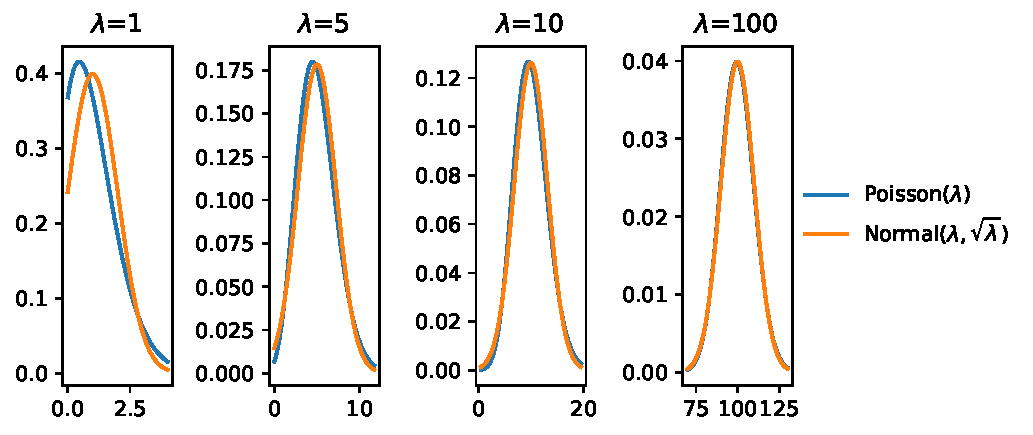
\includegraphics{./stat-fundamentals_files/figure-pdf/fig-poisson-output-1.pdf}

}

\caption{\label{fig-poisson}Comparison of the Poisson distribution at
different values of \(\lambda\) with a normal distribution with mean
\(\lambda\) and variance \(\sqrt{\lambda}\).}

\end{figure}

\hypertarget{uniform}{%
\subsubsection*{Uniform}\label{uniform}}

The \textbf{uniform} distribution is a very simple construct, with pdf

\[
    p(x | a, b) =
\begin{cases}
    \frac{1}{b-a},& \text{if } x\in [a,b]\\
    0,              & \text{otherwise}
\end{cases}
~.
\]

We'll use the shorthand of \(\mathrm{Uniform}(a,b)\). When we refer to
drawing values ``at random'', we're probably referring to drawing
\(x\sim \mathrm{Uniform}(0,1)\).

\hypertarget{sec-nps}{%
\subsection{Nuisance parameters}\label{sec-nps}}

When our probability model \(p(x|\mu)\) fails to describe the data
generating process well, we may add more parameters to our model in
order to make it more flexible, and thereby hopefully increase the
accuracy of the model. As an example, this could be a parameter that
controls the shape of the overall distribution in a way that models a
physical effect. Such parameters are called \textbf{nuisance
parameters}, as they exist only to add model flexibility (we're not
interested in inferring their true values), and are then a nuisance to
deal (increased dimensionality of any downstream calculations). If we
denote the set of nuisance parameters of a model as \(\theta\), our
likelihood then reads \(p(x|\mu,\theta)\).

If we have some prior knowledge about \(\theta\), e.g.~from a previous
experiment that measured the physical event on data \(y\) (termed
``auxillary data'' since it isn't directly to do with our main
experiment), it would be useful to use that to constrain possible values
\(\theta\) could take. In a Bayesian setting, this prior knowledge can
be added when defining the prior distribution for that parameter at
inference time. It's also possible to bake this information into the
probability model itself through constructing the joint likelihood of
both experiments:

\[p(x, y|\mu,\theta) = p(x|\mu,\theta)p(y|\theta) ~.\]

In the case where the distribution \(p(y|\theta)\) isn't readily
available, it's common practice in HEP to approximate it using a
distribution that models the shape of the data \(y\) to some reasonable
degree of accuracy, e.g.~with a normal distribution of mean \(\theta\)
(this will be discussed more later).

To extract information about parameters of interest \(\mu\) from a
likelihood that involves \(\theta\), we need to somehow lose our
dependence on \(\theta\) to recover a distribution that just depends on
\(\mu\). The ways of doing this are as follows:

\textbf{Profiling}: for each value of \(\mu\), find the best fit value
of \(\theta\), leading to

\[ p_{\mathrm{profile}}(x|\mu) = p(x | \mu, \hat{\hat{\theta}});\quad\hat{\hat{\theta}}=\underset{\theta}{\mathrm{argmax}}(p(x|\mu,\theta))~.\]

Here, we're essentially picking our best guess of the value of the
nuisance parameters given a specified \(\mu\). The profile likelihood
will obviously be useful in the limit of \(\hat{\hat{\theta}}\) being
close to the true values of the nuisance parameters, but this isn't
guaranteed.

\textbf{Marginalization}: we simply integrate away the dependence on the
nuisance parameters entirely:

\[p_{\mathrm{marginal}}(x|\mu) = \int_{-\infty}^{+\infty} p(x| \mu, \theta) p(\theta) d\theta ~.\]

Note that this requires a specification of a prior pdf \(p(\theta)\).
Marginalizing is then a form of averaging of the likelihood and prior
across the domain of \(\theta\). Despite this technically being a
Bayesian procedure due to the specification of the prior, we're free to
use the resulting model in a frequentist way -- this is just a model
specification step.

\hypertarget{metrics-of-probability}{%
\section{Metrics of probability}\label{metrics-of-probability}}

\hypertarget{sec-fisher}{%
\subsection{Fisher information and the Cramér--Rao
bound}\label{sec-fisher}}

A useful quantity in many ways is the \textbf{Fisher information
matrix}. We can write the definition for an element of this matrix for a
likelihood function \(p(x ; \theta)\) (\(\theta = \{\theta_i\}\)) as

\[
\mathcal{I}(\theta)_{ij}=-\frac{\partial^2}{\partial \theta_i \partial \theta_j} \log p(x ; \theta)~.
\]

We'll focus on the fact that you can extract \emph{parameter uncertainty
estimates} from this quantity. How? We turn to the Cramér--Rao bound,
which states that if we have an unbiased estimator for the likelihood
parameters \(\hat{\theta}\), the Fisher information matrix
\(\mathcal{I}(\theta)\) satisfies

\begin{equation}\protect\hypertarget{eq-cramer-rao}{}{
\Sigma_{\hat{\theta}^2} \geqslant [\mathcal{I}(\theta)]^{-1}~,
}\label{eq-cramer-rao}\end{equation}

where \(\Sigma_{\hat{\theta}}^2\) is the covariance matrix for the
fitted parameters \(\hat{\theta}\). In the asymptotic limit, the maximum
likelihood estimator will attain this lower bound, and satisfies

\[
\sqrt{n}(\hat{\theta}-\theta) \rightarrow \text{Normal}(0, [\mathcal{I}(\theta)]^{-1})~
\]

for sample size \(n\). A useful thing about this is that the diagonal
elements of the inverse Fisher information will then correspond to the
variances of the individual parameters,
i.e.~\([\mathcal{I}(\theta)]^{-1}_{ii} = \sigma_{\theta_i}^2\). There
are also many other interesting quantities we can extract from this
equivalence, including the \emph{generalized variance}, which is the
determinant of the covariance matrix (or determinant of the inverse
Fisher information). These quantities will see a little use later on.

\hypertarget{sec-KL}{%
\subsection{Kullback-Leibler divergence}\label{sec-KL}}

The \textbf{Kullback-Leibler divergence} (KL divergence) is a commonly
used quantity in machine learning and information theory to represent
the ``distance'' between a probability distribution \(p(x)\) and an
estimation of that distribution \(q(x)\). Related to things like
entropy, it can be thought of as the loss of information from using
\(q\) as an approximation to \(p\). It's defined for continuous \(x\) as

\begin{equation}\protect\hypertarget{eq-kl-divergence}{}{
D_{KL}(p(x) \| q(x))=\int_{-\infty}^{\infty} p(x) \ln \frac{p(x)}{q(x)} dx~.
}\label{eq-kl-divergence}\end{equation}

One interesting thing to note is that this is not a distance in the
typical sense, since it's an \emph{asymmetric} number,
i.e.~\(D_{KL}(p(x) \| q(x)) \neq D_{KL}(q(x) \| p(x))\).

\hypertarget{inference}{%
\section{Inference}\label{inference}}

\textbf{Statistical inference} can be viewed as the inverse of the data
generating process. Let's look at an example.

Say that the Lorax created the Earth. Moreover, say that he did so by
rolling a six-sided die, and putting the result of the die into a World
Generating Machine, which merely requires a single number as input. As a
neutral party that cannot confirm the Lorax's roll, but can definitely
observe the outcome, we may wonder: assuming we have a model of the
World Generating Machine, what number did the Lorax roll to produce all
that we see around us today? Moreover, can we factor in our prior
suspicion that a Lorax rolled a die to select a number at random?

Put in a more general way: given a parametrized model of the world
around us, potential suspicions about the parameters themselves, and
some data that could be described by that model, which values of the
parameters could have produced the data? Moreover, is the model a good
description of the data at all? Could another model have described the
data more accurately? These type of questions fall within the umbrella
of statistical inference.

Let us add a layer of specificity to our questions. The key inquiries
that are typically dealt with through inference are:

\begin{itemize}
\tightlist
\item
  \textbf{Point estimation}: What value(s) of my model parameters best
  describe the data?
\item
  \textbf{Interval estimation}: How can I specify a plausible range for
  my model parameters based on the data they attempt to describe? (One
  can obtain a symbiotic relation between interval and point estimation
  by viewing a point estimate as the limit of shrinking intervals)
\item
  \textbf{Hypothesis testing}: Given a model of the data generating
  process, to what extent does it describe the data when\ldots{}

  \begin{itemize}
  \tightlist
  \item
    \ldots compared to another model with different form?
  \item
    \ldots compared to the same model with different parameters?
  \item
    \ldots not being compared to any particular alternative? (this has
    the particular name of the \emph{goodness-of-fit test})
  \end{itemize}
\end{itemize}

These questions are where the schools of probability see their strongest
divide; whether we can assign probabilities to facts -- e.g.~what are
the odds that neutrinos have masses -- fundamentally alters the kind of
question we can ask of our model/data. For example, instead of a point
estimate of the neutrino masses, a Bayesian procedure could infer their
\emph{distribution} given the data (and some prior beliefs about their
values), also termed the \emph{posterior distribution}. Similarly,
Bayesian intervals can say ``what are the chances the true parameter
value lies in this interval'' (which frequentist procedures \emph{can
not determine}), and hypothesis testing can evaluate the probability of
the hypothesis itself.

However, these Bayesian procedures undertake the weight of the
specification of a prior distribution for all of these quantities, which
will (in the limited data regime, a.k.a. real life) strongly affect the
result. Moreover, the frequentist procedures are indeed still useful for
making exact, even if convoluted, statements about the model in the
presence of observed data.

A brief aside: you'll notice that the common thread throughout these
statements is the \emph{model}. As like many statistics-adjacent HEP
researchers before me, I will emphasize that \emph{the likelihood model
is the most important ingredient for any inference procedure}. In the
limit of a well-designed model and sufficient data, even a room full of
the most polarized statisticians, hopelessly resigned to their
particular school of thought, will agree on basic statements about the
validity of a hypothesis. Even failing this,a Bayesian would not ignore
a \(p\)-value of 0.9, and a frequentist would likewise raise their
eyebrows at a flat or sharp posterior with low prior sensitivity. But
since they both care about the model, any and all effort that could be
spent arguing over inferencial philosophy may likely be better placed in
talking to a domain expert for the problems you care about.

But enough with the aside, or I'll be subject to the same criticism of
misplaced effort. Let's review the different methods that implement
answers to our questions of inference.

\hypertarget{sec-mle}{%
\subsection{Point estimation}\label{sec-mle}}

Given a probability model \(p(x|\mu)\) for data \(x\) and model
parameters \(\mu\), the most common method of estimating parameter
values compatible with observed data \(x_0\) in the frequentist paradigm
is the \textbf{maximum likelihood estimate} (MLE), defined as

\[ \hat{\mu} = \underset{\mu}{\mathrm{argmax}}(p(x_0|\mu))~.\]

In practice, we calculate \(\hat{\mu}\) with an optimization procedure,
e.g.~through the (L)BGFS algorithm for unconstrained optimization
(Fletcher 1987). Since most optimization algorithms target minimization
(purely conventional), we often frame this equivalently as

\[ \hat{\mu} = \underset{\mu}{\mathrm{argmin}} (-2\ln p(x_0|\mu))~.\]

The prefactor of 2 leads to some nice theoretical properties via Wilk's
theorem, but that's a later discussion (the 2 doesn't matter for
optimization purposes). We calculate the MLE lot in HEP for a few
reasons:

\begin{itemize}
\tightlist
\item
  It has a \emph{Normal sampling distribution} in the asymptotic limit
  (so we can easily quote errors using a sample standard deviation)
\item
  In the finite data regime, the MLE is effective for many distributions
  we care about (e.g.~Normal, Poisson)
\item
  Simple to understand and debug!
\end{itemize}

Other methods of point estimation could be as simple as quoting the
\emph{mode} (value with highest density), \emph{median} (value that
partitions the distribution into equal segments of probability), or
\emph{arithmetic mean} (sum of the data divided by the size of the
data). These are more useful in the absence of a good probability model.

\hypertarget{sec-conf-intervals}{%
\subsection{Confidence intervals}\label{sec-conf-intervals}}

A significant part of my early PhD days was spent trying to understand
the confidence interval. I will do my best to try and make you bang your
head against the wall a little less than me (metaphorically, I hope).

We begin with some statistic of the observed data \(x\). A confidence
interval is then a statement about values of a model parameter \(\mu\)
for which the observed data is considered \emph{``not extreme''}. Values
of \(\mu\) outside the interval are then those for which the observed
data is \emph{``extreme''}. We have a couple of ingredients to unpack
here:

\begin{itemize}
\tightlist
\item
  How do we define a notion of ``extreme'' for the data?
\item
  How do we construct the interval itself to satisfy this property
  (namely that the values of \(\mu\) consistently treat \(x\) as extreme
  or not)?
\end{itemize}

For the first point, there's a two-part answer: we need a way to order
the data with a notion of extremity (rank it from least to most
extreme), and then also determine the cutoff for which points are
considered extreme or not. This cutoff isn't going to be by value, but
by \emph{proportion}; we'll place our yardstick such that all values of
\(x\) considered \emph{not} extreme contain the majority of the
probability (area under \(p(x|\mu)\)). How much? That's known as the
\textbf{confidence level} (\(\mathrm{C.L.}\)). Values considered
\emph{extreme} then occupy the other \(1-\mathrm{C.L.}\) of the
probability. We then determine those values of \(\mu\) which produce
distributions that satisfy this requirement \emph{when the yardstick is
in the same place as the observed data \(x_0\)}. We'll see some examples
of this below.

For 1-D \(x\), we look at some simple orderings: - \emph{Descending}:
large \(x\) is not considered extreme, and small \(x\) is. The
corresponding confidence interval is
\([\mu_{\mathrm{lower}}, +\infty]\), where \(\mu_{\mathrm{lower}}\) is
known as a \textbf{lower limit} on \(\mu\). - \emph{Ascending}: small
\(x\) is now not extreme, but large \(x\) is. The corresponding
confidence interval is \([-\infty, \mu_{\mathrm{upper}}]\), where
\(\mu_{\mathrm{upper}}\) is known as an \textbf{upper limit} on \(\mu\).

We can also look at a \emph{central} ordering, which produces an
interval that can be constructed at a given confidence level
\(\mathrm{C.L.}\) through calculating a lower and upper limit
\([\mu_{\mathrm{lower}}, \mu_{\mathrm{upper}}]\), each with a confidence
level of \(1-(1-\mathrm{C.L.})/2\) (which guarantees that the central
interval contains \(\mathrm{C.L.}\) of the probability).

Let's make this concrete with an example: we'll take the same
distribution studied in (Cousins 2018) (Section 6.4), where we have a
normal distribution with width parametrized as 1/5th of the mean:

\[x \sim \mathrm{Normal}(\mu, \frac{\mu}{5}).\]

From here, we can examime the pdf (at \(\mu=10\) arbitrarily). We can
also view the likelihood if we say we observed data \(x_0=10\). Both are
shown in Figure~\ref{fig-density}.

\begin{figure}

{\centering 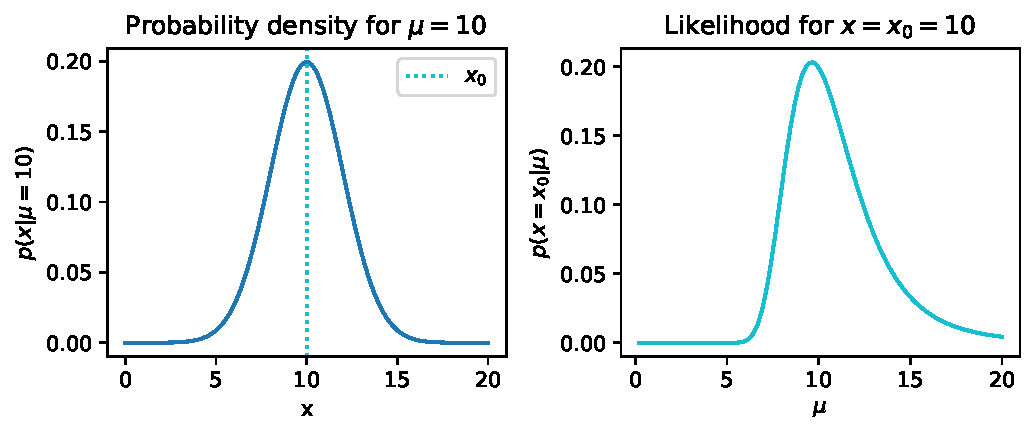
\includegraphics{./stat-fundamentals_files/figure-pdf/fig-density-output-1.pdf}

}

\caption{\label{fig-density}Probability density function and likelihood
for different assumed values of \(x\) and \(\mu\).}

\end{figure}

Let's now use the aforementioned method to construct a central
confidence interval for \(\mu\), at say a confidence level of 68.3\%. We
then divide up this confidence level into the lower and upper limits --
each will be set with a confidence level of \(1-(1-0.683)/2 = 84.15\%\),
such that the extreme data occupies one minus that amount (15.95\%) of
the probability on each side of the central interval, giving us back the
desired 68.3\% between the upper and lower limits.

Finding these limits can be viewed as an optimization problem: we just
need to choose \(\mu\) such that the area under \(p(x|\mu)\) is equal to
84.15\% \emph{below} \(x_0\) for lower limits, and \emph{above} \(x_0\)
for upper limits. We can frame this objective using the cumulative
density function -- the cdf evaluated at \(x_0\) must be equal to 0.843
for lower limits, and equal to 1-0.843 for upper limits. As this thesis
focuses on methods relating to gradient descent, we can use this to find
our central interval, by optimizing \(\mu\) with respect to a
mean-squared error loss between the cdf and the relevant probability
share. Doing this for our example gives us the limits {[}8.332,
12.502{]} that form a central confidence interval for \(\mu\).

We can visualize the probability density for each of
\(\mu_{\mathrm{lower}}\) and \(\mu_{\mathrm{upper}}\), which should help
cement the idea of capturing some amount of the probability up to
\(x_0\) based on an ordering of \(x\):

\begin{figure}

{\centering 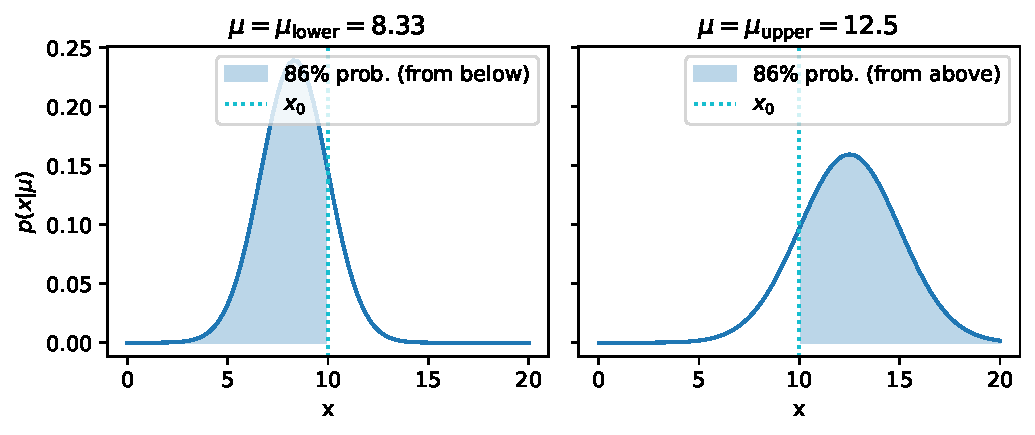
\includegraphics{./stat-fundamentals_files/figure-pdf/fig-uplow-output-1.pdf}

}

\caption{\label{fig-uplow}Probability density functions at both
\(\mu_{\mathrm{lower}}\) and \(\mu_{\mathrm{upper}}\), showing that the
enclosed area under the curve at \(x_0\) equals the desired amount as
dictated by the confidence level.}

\end{figure}

\hypertarget{neyman-construction}{%
\subsubsection*{Neyman construction}\label{neyman-construction}}
\addcontentsline{toc}{subsubsection}{Neyman construction}

A different way to build confidence intervals (that generalizes to
multiple dimensions) can be found in the form of the \textbf{Neyman
construction}. Here, we start by constructing an \emph{acceptance
interval} for \(x\). Given an ordering of \(x\), a desired confidence
level \(\mathrm{C.L.}\), and a value of \(\mu\), an acceptance interval
for \(x\) is defined such that the probability contained between
\([x_1, x_2]\) is equal to \(\mathrm{C.L.}\). In equation form:

\[ [x_1, x_2]~s.t.~P(x\in[x_1,x_2] | \mu) = \mathrm{C.L.} .\]

The endpoints \([x_1, x_2]\) are well defined because we decided on an
ordering for \(x\) (does not need to be central!), with any data outside
these endpoints designated as ``extreme'' with respect to that ordering.

We can then draw the acceptance intervals for many values of \(\mu\).
This can be visualized in a plot of \(\mu\) against \(x\) as a set of
horizontal lines in \(x\) corresponding to the acceptance intervals. How
do we turn this into an interval on values of \(\mu\)? We just draw a
vertical line corresponding to our observed data \(x_0\), and choose the
values of \(\mu\) that lie where the line intercepts the acceptance
intervals for \(x\). All of this is shown in Figure~\ref{fig-neyman}.

\begin{figure}

{\centering 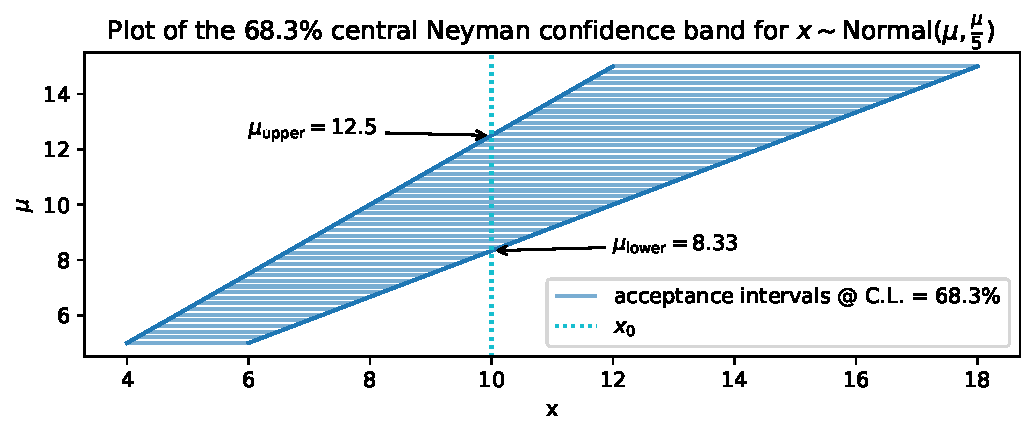
\includegraphics{./stat-fundamentals_files/figure-pdf/fig-neyman-output-1.pdf}

}

\caption{\label{fig-neyman}Neyman confidence band, showing both the
overall envelop and explicit acceptance intervals in \(x\). Also shows
how one can then determine \(\mu_{\mathrm{lower}}\) and
\(\mu_{\mathrm{upper}}\) at the intersection of the band and observed
data \(x_0\).}

\end{figure}

Even though the appearance of the plot in Figure~\ref{fig-neyman} makes
it look so, it is completely \emph{not required that \(\mu\) be 1-D!}
For example, \(\mu\) could easily have been 2-D here, and then the
confidence interval in 2-D could still be constructed by the points at
which the observed data (which would be the plane defined by \(x_0=10\))
meets the acceptance intervals, even if this stretches out over other
parameter dimensions. What happens if that multi-dimensional space
becomes even larger, even if we don't care about some of the parameters?
We'll look at new ordering principle for this.

\hypertarget{likelihood-ratio-ordering}{%
\subsubsection*{Likelihood ratio
ordering}\label{likelihood-ratio-ordering}}
\addcontentsline{toc}{subsubsection}{Likelihood ratio ordering}

A fourth ordering principle for the data was proposed by Feldman \&
Cousins in (Feldman and Cousins 1998), and is based on the likelihood
ratio

\[ R(x, \mu) = \frac{p(x|\mu)}{p(x| \hat{\mu})} ,\]

where \(\hat{\mu}\) represents the best-fit value of \(\mu\). Commonly
used in HEP, it appeals to intuition since there's then a correspondence
between the notion of ``extreme'' and low probability density (relative
to the maximum). Moreover, since it's a ratio, a change in variables
from \(x\) to \(f(x)\) would lead to the Jacobians cancelling in \(R\),
making this ordering invariant to a change of metric. We can construct
intervals ordered by \(R\) through the Neyman method as above.

\hypertarget{profiling}{%
\subsubsection*{Profiling}\label{profiling}}
\addcontentsline{toc}{paragraph}{Profiling}

In the case where the likelihood parameters can be split into
\([\mu, \theta]\), with \(\theta\) representing nuisance parameters, we
can make this interval construction more feasible by using the
\textbf{profile likelihood ratio}:

\begin{equation}\protect\hypertarget{eq-profile-lhood-ratio}{}{
\lambda(x, \mu) = \frac{p\left(x|\mu,\hat{\hat{\theta}}(\mu)\right)}{p\left(x| \hat{\mu}, \hat{\theta}\right)},
}\label{eq-profile-lhood-ratio}\end{equation}

where \(\hat{\hat{\theta}}(\mu)\) represents the fitted value of
\(\theta\) when holding \(\mu\) fixed. Doing this reduces the
dimensionality of the parameter space to just those of which we're
interested in (e.g.~signal strength). However, coverage properties for
intervals constructed in this way may vary, so need to have their
sampling properties studied (see section 13 in (Cousins 2018)).

\hypertarget{coverage}{%
\subsubsection*{Coverage}\label{coverage}}
\addcontentsline{toc}{subsubsection}{Coverage}

Despite that a confidence interval is in values of \(\mu\), it's an
inherently \emph{data-dependent construct} -- you'll get a different
confidence interval for different observed data \(x_0\). The endpoints
of the interval \([\mu_{\mathrm{lower}}, \mu_{\mathrm{upper}}]\) are
consequently treated as random variables. The confidence level, then, is
a property of the set of intervals that would be constructed over many
experiments: if we sampled \(x\) from the true distribution many times
with many experiments, and constructed a confidence interval using each
sample with confidence level of 95\%, then 95\% of those intervals would
contain (or \textbf{cover}) the true value of \(\mu\). The collection of
these confidence intervals is called a \textbf{confidence set}, and we
say that it has 95\% \textbf{coverage}.

How do we know our confidence set has this property? Well, the Neyman
confidence set has it by definition: if we think about just the single
distribution at the true value \(\mu_T\), the Neyman procedure creates
an acceptance interval such that the probability between \([x_1, x_2]\)
is equal to the confidence level (say 95\%). If we then do many
experiments (i.e.~sample \(x\sim p(x | \mu_T)\)), we know that 95\% of
the time, the dotted line representing the data point will lie within
the acceptance interval of \(\mu_T\). Ah -- this is exactly the
requirement for \(\mu_T\) to be included in our confidence interval! It
then follows that 95\% of the \emph{intervals} constructed will then
include the true value of \(\mu\), corresponding exactly to when the
observed data lies within the acceptance interval for \(\mu=\mu_T\).

This is all well and good, but may ring some alarm bells -- we only have
one interval in practice, right? Isn't there a chance that we draw data
such that the confidence interval falls in the 5\% that don't cover the
true, unknown value of \(\mu\), and thereby \emph{contradicting the
distribution that produced the data point}?

In short, yes. But that doesn't mean confidence intervals are useless --
a single 95\% interval is overwhelmingly more likely to contain the true
parameter value than not. Remember: we're always going to have inherent
uncertainty on the statements we make on unknown true parameter values
-- this uncertainty is expressed as a probability distribution for
Bayesian methods, and as a statement about sampling properties (results
in the limit of many repeated experiments) for frequentist methods.

\hypertarget{sec-hyptests}{%
\subsection{Frequentist hypothesis testing}\label{sec-hyptests}}

Hypothesis testing gives us a framework to make qualitative statements
about how extreme the observed data seems under a proposed theory, often
in comparison to various alternatives. Note we use ``extreme'' in the
same way as with confidence intervals, so we're going to need to
establish an ordering principle for the data. Let's go into more detail.

Once again, we concern ourselves with a statistic of the data \(x\) and
model parameters \(\mu\). Here we follow the conventions set out by
Neyman (again) and Pearson in (Neyman and Pearson 1933), and start with
the notion of a \textbf{null} hypothesis \(H_0\), which is the assumed
default model for the data. One would often take this to be the Standard
Model, for example. We then come up with an alternative hypothesis
\(H_1\). In what way can \(H_0\) and \(H_1\) differ? We could have:

\begin{itemize}
\tightlist
\item
  Two totally separate probability models \(p_1(x | \mu_1)\) and
  \(p_2(x | \mu_2)\), which can differ in number of parameters and
  functional form
\item
  A set of hypotheses within a probability model; \(p(x | \mu)\) induces
  a family of hypotheses parametrized by \(\mu\), for instance, with any
  two values of \(\mu\) potentially serving as \(H_0\) and \(H_1\)
\end{itemize}

A hypothesis at a point (e.g.~\(p(x | \mu=0)\)) is known as a
\textbf{simple hypothesis}, and a set of hypotheses (e.g.~a second,
unspecified model \(p_2(x | \mu)\), or \(p(x | \mu\neq0)\)) is known as
a \textbf{composite hypothesis}. In HEP, we're commonly testing a point
null of \(H_0\) = Standard Model (\(p(x | \mu=0)\)) against a composite
alternative of \(H_1\) = Something Else (\(p(x | \mu\neq0)\)). This
poses a challenge from an optimality perspective that we'll cover
shortly.

So, how do we actually do the testing itself? We'll need an ordering
principle to rank data from least to most extreme. To do this, we
usually concentrate on defining a good \textbf{test statistic} of the
data \(t(x)\), then fix an ordering of \(t(x)\) ascending (but other
orderings are possible, e.g.~two-tailed tests are centrally ordered in
\(t(x)\)). From there, we come up with a cutoff value \(t_c\) such that
data with \(t > t_c\) is seen as extreme. The proportion of the
probability held by these extreme values is known as the
\textbf{confidence level} or \textbf{test size} \(\alpha\).

Under \emph{which distribution} is this ordering and designation of
\(\alpha\) performed? We do this with the pdf of the test statistic
under the null hypothesis, \(p(t(x)|H_0)\). Importantly, this
distribution may not be known to us, and we may have to estimate it by
sampling many values of \(x \sim p(x|H_0)\), then calculate \(t(x)\) for
all of them, and estimate the density of the result. Moreover, without
this distribution, we don't know how to place our cutoff \(t_c\) so it
contains a proportion \(\alpha\) of the data considered most extreme!

One more thing we can deduce from the above: our statements on how
extreme the observed data appears are \emph{fundamentally under the
assumption that \(H_0\) is true.} Keep this in mind!

If the observed data \(x_0\) falls in the extreme proportion of possible
values, i.e.~\(t(x_0) > t_c\), we then say we \emph{reject} \(H_0\)
compared to \(H_1\). Note that this does \emph{not mean we accept
\(H_1\)!} For that, we'd have to look at decision theory, which involves
establishing the notion of probabilities for \(H_0\) and \(H_1\), which
is beyond the scope of this frequentist testing framework (a more
detailed discussion can be found in e.g. (Cousins 2018), Section 3.4).

So if our testing revolves around \(H_0\), where does the alternative
\(H_1\) come into play? We can see the presence of \(H_1\) in commonly
used orderings, such as the \emph{likelihood ratio} of the two
hypothesis: \(t(x, \mu) = p(x | H_0)/p(x|H_1)\). Furthermore, we can
define a measure of \emph{error} in relation to \(H_1\): given \(H_1\)
is true, what's the probability of accepting \(H_0\), even when the data
come from \(H_1\)? This quantity is known as \(\beta\) -- a
\emph{powerful} test would have low \(\beta\), i.e.~often rejects
\(H_0\) in favour of \(H_1\) when it is true, leading to the quantity
\(1-\beta\) being known as the \textbf{power} of a test.

\begin{figure}

{\centering 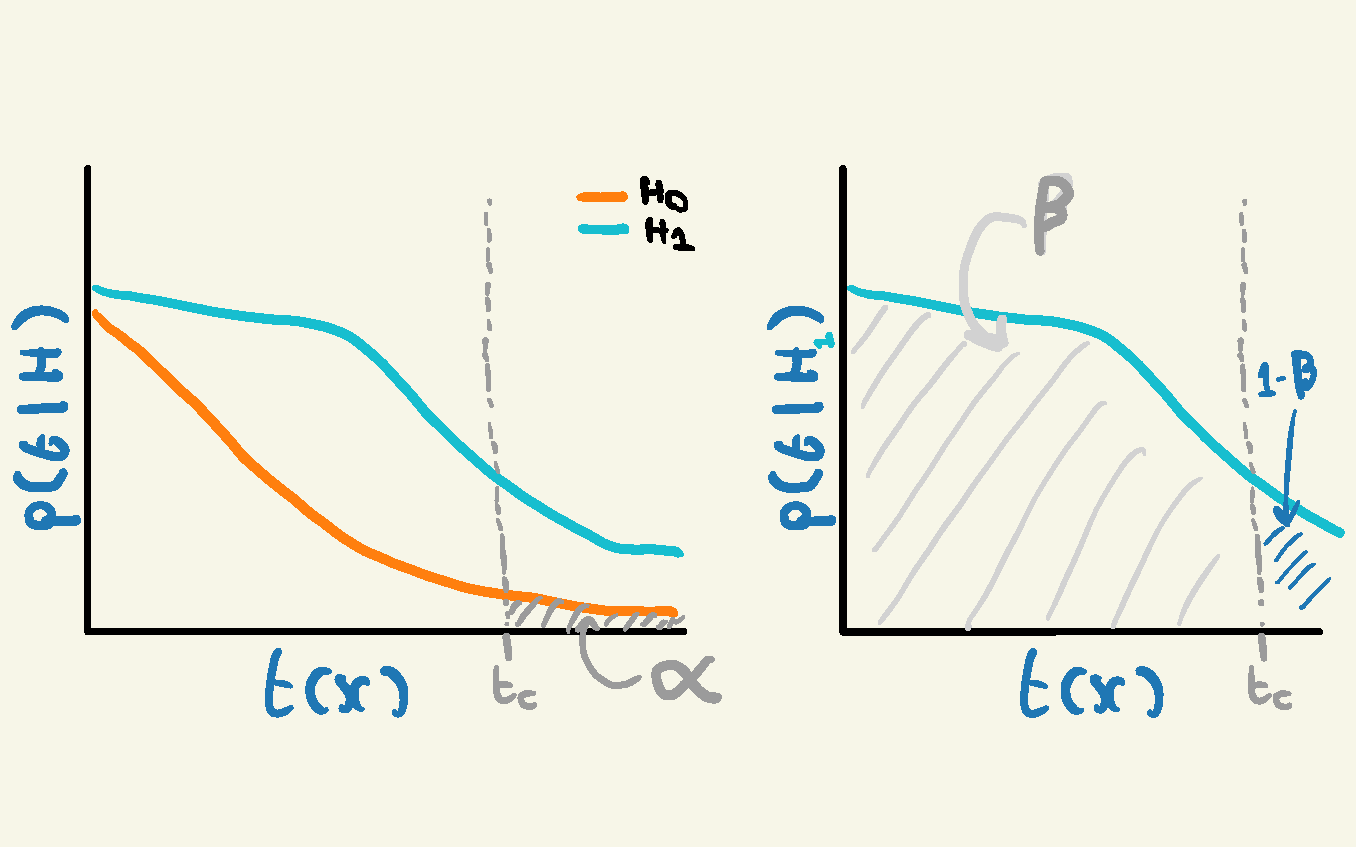
\includegraphics{./images/alphabeta.pdf}

}

\caption{\label{fig-visualtest}Visualization of a hypothesis test}

\end{figure}

When framing things in terms of error, we can see that the confidence
level \(\alpha\) also represents an error: \emph{the probability of
rejecting \(H_0\) given that it's true.} Why? If the observed data was
truly generated from \(H_0\), it will fall in the extreme proportion of
the data exactly \(\alpha\) of the time, since that's the way we
designated the proportions to begin with. This would lead to the
erroneous statement of rejecting \(H_0\) (though we know this stops
short of a \emph{decision} on \(H_1\)). We can see a representation of
both \(\alpha\) and \(\beta\) in Figure~\ref{fig-visualtest}.

The quantities \(\alpha\) and \(\beta\) are often called \emph{type-I}
and \emph{type-II} error respectively. I forget this all the time (in
particular which type means what) so rarely use these names, but include
them for completeness.

\hypertarget{p-values}{%
\subsubsection*{\texorpdfstring{\(p\)-values}{p-values}}\label{p-values}}
\addcontentsline{toc}{subsubsection}{\(p\)-values}

So we set up a test by choosing the size \(\alpha\), obtain the
distribution for our chosen test statistic \(t(x)\), and calculate the
cutoff value \(t_c\). What next? We'll take our observed data \(x_0\),
calculate \(t(x_0)\), and see if it lies past \(t_c\). If so, we'll
reject \(H_0\). If so, we'd maybe like to know by how much the data was
incompatible with \(H_0\). This quantity is known as the \(p\)-value,
and is just the area under \(p(t(x) | H_0)\), i.e.

\[ p_{x_0} = \int_{x_0}^{+\infty}p(t(x) | H_0) dx ~.\]

Note that the quantity \(p_{x}\) exists generally for \(x\) -- this is
just a rephrasing of the data into units that tell us how much of the
test statistic distribution we're enclosing to the right under \(H_0\).
\(p_{x_0}\) is then this statement for the observed data.

We can then rephrase a hypothesis test as rejecting \(H_0\) when
\(p_{x_0} < \alpha\), and accepting \(H_0\) otherwise. A low \(p\)-value
is then a sign of low compatibility between the observed data and
\(H_0\). (Here, my notation has come back to bite me\ldots{} \(p_{x_0}\)
is absolutely \emph{not} the probability of \(x_0\)!!!)

\hypertarget{optimality}{%
\subsubsection*{Optimality}\label{optimality}}
\addcontentsline{toc}{subsubsection}{Optimality}

What defines an optimal test? Well, \(\alpha\) is specified prior to the
test, so we're left with maximizing the \emph{power} \(1-\beta\). The
task then becomes: given \(\alpha\), choose a test statistic \(t(x)\)
such that the power \(1-\beta\) is maximized.

In the case where \(H_0\) and \(H_1\) are simple, the likelihood ratio
is the optimal test statistic in the sense of power, which can be proved
through the Neyman-Pearson Lemma (omitted here for the sake of brevity,
though see a visual proof in (Cranmer 2020)).

When we have a composite hypothesis, things get trickier, since we've
only worked out the best test statistic for two point hypotheses.
Instead of most powerful test, we need to change our language: we want
the \emph{uniformly most powerful test} across the many point hypotheses
contained within the composite hypothesis.

A proxy way to address this is the following: we know that the
likelihood ratio is optimal for two point hypothesis. If we're testing a
point null (\(\mu=\mu_0\)) against a composite alternative
(\(\mu \neq \mu_0\)), we can represent the alternative through the
\emph{best-fit hypothesis to the observed data}, i.e.~estimate
\(\hat{\mu}\) via maximum likelihood. We can then use the test statistic
\(p(x | \mu_0) / p(x | \hat{\mu})\). This is exactly analogous to the
use of a likelihood ratio ordering in confidence intervals!

\hypertarget{duality-between-hypothesis-test-and-intervals}{%
\subsection{Duality between hypothesis test and
intervals}\label{duality-between-hypothesis-test-and-intervals}}

It was probably hard to watch the number of times I defined ``extreme''
in this very specific way that seems to apply to both intervals and
tests, without commenting on how they're similar or different. That's
because they're one-to-one in many ways!

Say we make a \(\mathrm{C.L.}\) = 95\% confidence interval of
\([\mu_1, \mu_2]\) given an ordering principle/test statistic
(e.g.~likelihood ratio), a pdf \(p(x | \mu)\), and some observed data
\(x_0\). This interval contains all values of \(\mu\) for which the
observed data \(x_0\) is deemed \emph{not} extreme. Given the \emph{same
ordering principle}, a hypothesis test of some particular \(\mu_0\)
asks: does \(x_0\) lie in the extreme fraction of data
\(\alpha = 1-\mathrm{C.L.}\) when \(\mu=\mu_0\)? This is the \emph{same
thing} as asking: does \(\mu_0\) lie in the confidence interval
\([\mu_1, \mu_2]\)? If so, then the acceptance interval for
\(p(x | \mu_0)\) will be intercepted by \(x_0\) -- this would
\emph{accept} \(H_0\) in the testing framework, since \(x_0\) under
assumption of \(\mu_0\) is not considered extreme.

I hope this is clear enough, it took me a little while to see initially!
One can then \emph{invert a test} to produce a related confidence
interval, which just means taking the set of \(\mu\) that aren't
rejected in a test using the observed data:

\[ \{\mu: t(x_0, \mu) < t_c \} = \mathrm{confidence~interval~at~C.L.~of~}1-\alpha ~.\]

\hypertarget{sec-bayes}{%
\subsection{Bayesian procedures}\label{sec-bayes}}

I won't talk much about the Bayesian methodology here since I didn't
explicitly use it in my PhD, but it's worth mentioning for contrast.
Moreover, if you're a student within HEP reading this, I don't want to
make it seem like there's only one way of doing things -- there are
analyses that use these methods, and I think they should be explored
more! See something like (Sivia and Skilling 2006) for a comprehensive
introduction.

As I've mentioned a few times, the Bayesian interpretation of
probability admits distributions for facts; one can ask ``how likely is
supersymmetry?'' or ``what's the distribution for my signal strength?''
These questions are often answered via use of Bayes theorem, which
states that for probability distribution \(p(\cdot)\), data \({x}\), and
model parameters \({\mu} = \{ \mu_1, \mu_2, \dots, \mu_n\}\), \[
p({\mu}|{x}) = \frac{p({x}|{\mu})p({\mu})}{p({x})}~.
\]

We call \(p({\mu}|{x})\) the joint \textbf{posterior} distribution of
the parameters \({\mu}\), since it reflects our updated beliefs
post-data. We know about the likelihood \(p(x|\mu)\), but \(p({\mu})\)
(the product of the individual distributions \(p(\mu_i)\)) is a new
player in the game: these are the \textbf{prior} distributions for each
parameter, called as such to reflect our prior belief in their
distributions. We need to incorporate this information to perform
inference using this paradigm, which is often a difficult task to do
faithfully (even when we want to claim ignorance). Finally, the
normalizing factor \(p({x})\) is termed the \textbf{model evidence}, and
is obtained by marginalizing out the model parameters:

\[
\mathrm{Evidence} = \int_\Omega p({x}|\mu)\times p(\mu)\,\mathrm{d}\mu
\] over parameter domain \(\Omega\). Often, Bayesian computation only
requires proportionality with respect to the parameters, so it's common
to just think of the equation

\[
\mathrm{Posterior} \propto \mathrm{Likelihood} \times \mathrm{Priors}
\] as the defining equation of Bayesian inference, though the model
evidence remains useful as a compatibility measure between data and
likelihood.

One thing to note: Bayes theorem does not use the Bayesian definition of
probability unless we decide to -- it's derived from the axioms of
probability, and is thus invariant of interpretation. Using this theorem
in a Bayesian way only holds when we have a true but unknown quantity
(e.g.~\(\mu\)) as the subject of our distribution, as is done here.

Armed with this equation, Bayesian procedures include:

\begin{itemize}
\tightlist
\item
  \textbf{Posterior estimation} (e.g.~through Markov chain monte carlo
  and it's variants)

  \begin{itemize}
  \tightlist
  \item
    Can then perform point estimation via \emph{maximum a posteriori}
    (the mode of the posterior)
  \end{itemize}
\item
  \textbf{Credible intervals}: in contrast to confidence intervals where
  the endpoints are random variables, \(\mu\) itself is now the random
  variable, and the interval is constructed such that it contains the
  true value \(\mu_T\) with some allocated probability.
\item
  \textbf{Hypothesis testing}: Bayesian hypothesis tests do exist, and
  involve the model evidence; I won't talk about them here.
\item
  \textbf{Evidence estimation}, e.g.~nested sampling (Skilling 2006),
  which also comes with a posterior estimate as a by-product.
\end{itemize}

\hypertarget{probability-and-statistics-in-practice}{%
\chapter{Probability and Statistics, in
practice}\label{probability-and-statistics-in-practice}}

This section focuses on how fundamental statistical ideas are translated
into meaningful physics insights. We'll look at common practice, and
summarize the main components needed to set the scene for applications
that involve building new ideas with these techniques.

My primary resources for this section were the seminal asymptotics paper
(Cowan et al. 2011) and Kyle Cranmer's stats notes (Cranmer 2014).

\hypertarget{estimating-distributions-from-data}{%
\section{Estimating distributions from
data}\label{estimating-distributions-from-data}}

Often we're not equipped with a way to describe some data we're
interested in using a probability distribution. In that situation, it's
useful to have a set of \textbf{density estimation} techniques within
your toolkit. Here we go over a couple.

\hypertarget{sec-hists}{%
\subsection{Histograms}\label{sec-hists}}

Ah yes, the infamous histogram. Exceedingly simple by design, it
approximates a data distribution through counting the number of data
points that lie in a set of adjacent disjoint intervals, or
\textbf{bins}. A histogram, then, is expressible as a set of counts and
a set of bin edges. See some example histograms in Figure~\ref{fig-hist}
to see how the binning can affect the overall envelope of the
distribution.

\begin{figure}

{\centering 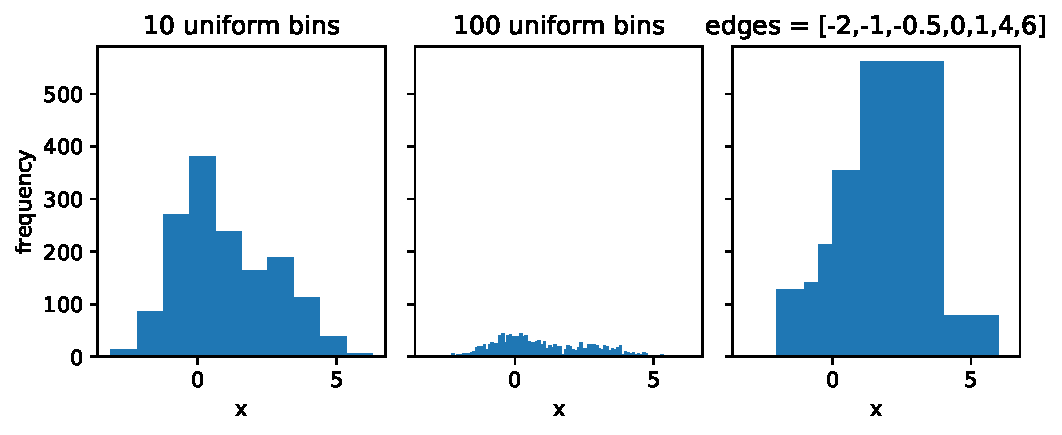
\includegraphics{./stat-practical_files/figure-pdf/fig-hist-output-1.pdf}

}

\caption{\label{fig-hist}Histogram of some bi-modal data \(x\), shown
with different binnings.}

\end{figure}

The area under the histogram is equal to
\(\sum_{\mathrm{bins~i}} \mathrm{count}_i \times \mathrm{bin~width}_i\);
we can force this to unit area by dividing each term in the sum by the
bin width and the total number of counts. This produces something that
can be interpreted as a (discrete) probability density, which can be
useful when looking at just the shape of the distribution, for instance.

\hypertarget{sec-whyhist}{%
\subsubsection*{Why histograms in HEP?}\label{sec-whyhist}}

I
\href{https://twitter.com/phi_nate/status/1251124042012274693?s=20\&t=_miEUw-BGQwuWl1rsgyHuQ}{asked
this question on Twitter} because I was confused: the HEP analysis
paradigm has the histogram as a central object, but why? The reasons I
discovered are as follows:

\begin{itemize}
\tightlist
\item
  \textbf{Data structures}: the histogram has many benefits as a vessel
  to store data, e.g.~their memory footprint is \emph{independent of the
  size of the input data} -- large numbers for the counts are still just
  single numbers! They also have effectively no cost to evaluate (you
  just look up the count number based on the bin)
\item
  \textbf{Poisson modelling}: a simple and tractable way to model the
  likelihood of a collider physics process is with a Poisson-based
  likelihood function, which has an expected number of counts that is
  parametrized using templates from signal and background processes.
  When you make a histogram of your physics quantities, you can model it
  in this way through having one Poisson distribution per bin!
\end{itemize}

There was also more in that thread on ease of parallel computation, the
fact that histograms are good at respecting physical boundaries, and
some birds-eye view perspectives on how things are (and could be) done
in the field. Many thanks to Kyle Cranmer, Jim Pivarski, Stan Seibert,
Nick Smith, and Pablo De Castro for contributing to that discussion -- I
encourage you to check out the thread!

\hypertarget{sec-kde}{%
\subsection{Kernel density estimation}\label{sec-kde}}

If you wanted a smooth distribution instead of a discrete one, the
\emph{kernel density estimate} (KDE) has you covered.

It's a pretty simple but powerful idea: for each data point, define some
\emph{kernel function} that uses the point as a centre (e.g.~normal
distribution). Then, the distribution of the data at a point \(x\) is
equal to the average of the kernel functions evaluated at \(x\).

There are many different choices of kernel function, each with their own
tradeoffs, but the most common one in practice is indeed the standard
normal distribution \(\mathrm{Normal}(0, 1)\). If we specify the mean as
the data, then there's one missing ingredient -- the \emph{width} of
these distributions. That number is called the \textbf{bandwidth}, and
controls the width of every kernel at once. Interestingly, the choice of
bandwidth affects the resulting shape in general much more than the
choice of kernel -- see Figure~\ref{fig-kde} for some examples of the
bandwidth's influence on the distribution.

\begin{figure}

{\centering 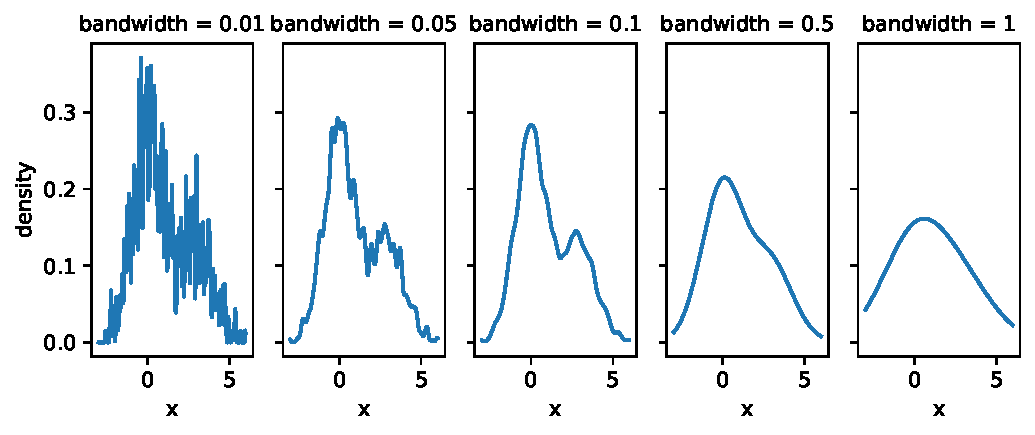
\includegraphics{./stat-practical_files/figure-pdf/fig-kde-output-1.pdf}

}

\caption{\label{fig-kde}KDE of some bi-modal data \(x\), shown with
different bandwidths.}

\end{figure}

Some talk on a midpoint between KDEs and histograms will appear in the
applications part of the thesis!

\hypertarget{fitting-an-existing-distribution}{%
\subsection{Fitting an existing
distribution}\label{fitting-an-existing-distribution}}

If you have a decent idea on a distribution that may reasonably describe
your data, you can simply perform a maximum-likelihood optimization to
fit the parameters of the model to the data. One can even compose
multiple distributions into a more complex likelihood. Not too much more
to say about this, as it essentially comes under point estimation of a
model parameter, which we talked about in the previous chapter!

\hypertarget{other-data-driven-methods}{%
\subsection{Other data-driven methods}\label{other-data-driven-methods}}

We'll talk more about these in the machine learning section,
e.g.~Gaussian processes and normalizing flows. These are generally
reserved for when you need a little bit of extra work in order to get a
robust result, or to go beyond 1-D and 2-D variables in a scalable way.

\hypertarget{sec-hifa}{%
\section{HistFactory: modelling nature as a set of
counts}\label{sec-hifa}}

HistFactory (Cranmer et al. 2012) is by far the most common statistical
modelling tool used for collider physics data analysis. It's known for
being difficult to understand at first -- if you've ever seen the full
expression for the general likelihood, you'll have wondered if there was
a need to extend the Greek alphabet to write down all the symbols that
are used. Here, we'll take a slower and more gentle approach, building
up the HistFactory likelihood piece-by-piece, until hopefully it's clear
enough what's going on.

\hypertarget{baseline-model-for-a-chosen-statistic}{%
\subsection{Baseline model for a chosen
statistic}\label{baseline-model-for-a-chosen-statistic}}

Given some (new) physics process exists, we may expect \(\lambda\)
events to appear in our detector from that process. This number could
come from e.g.~simulating the physics process. It could also come from
e.g.~some data driven extrapolation method, but I'm going to call all of
this simulation for the sake of the arguments below. The point is that
we estimate it before looking at the important data in the region that
would contain new physics.

So: say we run our detector, and we record \(n\) \emph{independent}
events. What's the likelihood of observing these \(n\) events with
\(\lambda\) expected from simulation?

We know from the previous chapter that this is modelled well with a
Poisson distribution:

\begin{equation}\protect\hypertarget{eq-poisson}{}{
p(n|\lambda) = \mathrm{Poisson}(n|\lambda)~.
}\label{eq-poisson}\end{equation}

Along with the overall number of events we recorded, we may pick some
statistic of the data \(x\) that we choose to measure. That variable
will have a distribution we can predict from simulation. How do we
describe it?

We know that our data is divided into two categories: stuff that came
from physics we're interested in (\textbf{signal}), and stuff that came
from everything else (\textbf{background}). We can then say we have
\(s\) signal events in our sample and \(b\) background events, with
\(s+b=\lambda\), our overall number of expected counts from simulation.

Each value of \(x\) that comes from a signal event can be viewed as a
sample from the unknown signal distribution \(f_s(x)\), and likewise for
background \(f_b(x)\). We can even think of any particular value we
measured (e.g.~\(x_0\)) as being ``marked'' with an extra number --
either \(f_s(x_0)\) if it came from signal, or \(f_b(x_0)\) if it
belongs to the background. This means that our overall distribution for
the variable \(x\) is described by ``\(s\)'' much of \(f_s(x)\), and
``\(b\)''-much of \(f_b(x)\), i.e.~for any value of \(x\), it's density
is then

\begin{equation}\protect\hypertarget{eq-balance}{}{
p(x) = \frac{sf_s(x) + bf_b(x)}{s+b}~,
}\label{eq-balance}\end{equation}

where we choose to normalize by the total number of events \(s+b\) to
treat \(p(x)\) as a proper density.

We can then model the whole dataset \(\{x_i\}_{i=1}^n\) by multiplying
the densities of all the individual events, since we assumed they were
independent (otherwise we couldn't use the Poisson distribution!). We
can then incorporate Equation~\ref{eq-poisson} with
Equation~\ref{eq-balance} through multiplication of the densities:

\begin{equation}\protect\hypertarget{eq-histcomb}{}{
p(\{x_i\}_{i=1}^n) = \mathrm{Poisson}(n|s+b)\prod_{i=1}^n\frac{sf_s(x_i) + bf_b(x_i)}{s+b}~.
}\label{eq-histcomb}\end{equation}

Notice that we don't have any free parameters right now -- the counts
\(s\) and \(b\) will be fixed from our physics simulation once we get
around to it. But what if wanted to infer the amount of signal present
in our data? How would we do that? We can accomplish this through a
little trick: we can multiply the number of signal events \(s\) with an
additional number \(\mu\) that controls the overall \textbf{signal
strength}. Estimating the value of \(\mu\) would then tell us
information about the amount of signal present in the data (assuming our
model is accurate enough)!

We can now replace \(s\) with \(\mu s\) in Equation~\ref{eq-histcomb} to
get

\begin{equation}\protect\hypertarget{eq-bothparts}{}{
p(\{x_i\}_{i=1}^n | \mu) = \mathrm{Poisson}(n|\mu s+b)\prod_{i=1}^n\frac{\mu sf_s(x_i) + bf_b(x_i)}{\mu s+b}~.
}\label{eq-bothparts}\end{equation}

In this formalism so far, we've kept things generalized to the
``unknown'' pdfs \(f_s(x)\) and \(f_b(x)\), but we don't actually have
access to them. We can approximate them using a KDE or some other
method, but it's more common to find us with a \emph{histogram} for this
representation (reasons for why are outlined in
Section~\ref{sec-whyhist}).

Say we histogram our simulated signal and background data with the same
binning (not required to be uniform) that uses a number of bins \(k\),
giving us sets of counts
\(\mathbf{h}^{\mathrm{sig}} = \{h_1^{\mathrm{sig}}, h_2^{\mathrm{sig}}, \dots, h_k^{\mathrm{sig}}\}\)
and
\(\mathbf{h}^{\mathrm{bkg}} = \{h_1^{\mathrm{bkg}}, h_2^{\mathrm{bkg}}, \dots, h_k^{\mathrm{bkg}}\}\).
Recall from Section~\ref{sec-hists} that we can use these to approximate
a density by normalizing with respect to bin width and number of events.
Then, if we say a given value of \(x\) falls into some bin with index
\(j\), we can write that the density at \(x\) is approximated by the
(normalized) count in that bin, for both signal and background
separately:

\[
f_s(x \in \mathrm{bin~}j) \approx \frac{h^{\mathrm{sig}}_j}{s\times\mathrm{width~of~bin}~j};~~~f_b(x \in \mathrm{bin~}j ) \approx \frac{h^{\mathrm{bkg}}_j}{b\times\mathrm{width~of~bin}~j}
\]

From here, we can express Equation~\ref{eq-bothparts} as a product over
bins \(j\) instead of events \(i\):

\[
p(\{n_j\}_{j=1}^k | \mu) = \mathrm{Poisson}(n|\mu s+b)\prod_{j=1}^k\frac{\mu h^{\mathrm{sig}}_j  + h^{\mathrm{bkg}}_j}{\mu s+b}~.
\]

Note that we've shifted from talking about values of \(x_i\) to bin
counts \(n_j\), where \(\sum_{j=1}^k n_i = n\). These counts don't seem
to appear in the likelihood yet, but we can make this explicit through
the following relation\footnote{This relation arises from noticing that
  \(\lambda^n = \lambda^{\sum n_j} = \prod_j \lambda^{n_j}\), and using
  it to manipulate the Poisson on the left-hand side, amongst other
  things. We gloss over the full working, but I would like to include it
  if I have time (reading this means I probably didn't, but I do plan to
  release a blog post in future).}:

\[
\mathrm{Poisson}(n|\mu s+b)\prod_{j=1}^k\frac{\mu h^{\mathrm{sig}}_i  + h^{\mathrm{bkg}}_i}{\mu s+b} \propto \prod_{j=1}^k \mathrm{Poisson}(n_j | \mu h^{\mathrm{sig}}_j  + h^{\mathrm{bkg}}_j)~,
\]

where the constant of proportionality is a factor involving factorials
of the individual counts (also referred to as combinatorics). Since we
don't care about the overall normalization when we do inference
(e.g.~the maximum likelihood value is independent of the scale, and the
normalization cancels in a likelihood ratio), we will consider this
proportionality as an equivalence.

These gymnastics have left us with the following likelihood:

\begin{equation}\protect\hypertarget{eq-hifabase}{}{
p(\{n_j\}_{j=1}^k | \mu) = \prod_{j=1}^k \mathrm{Poisson}(n_j | \mu h^{\mathrm{sig}}_j  + h^{\mathrm{bkg}}_j)~,
}\label{eq-hifabase}\end{equation}

which is simply a product over Poisson distribution for each bin within
a histogram, where we expect a contribution of
\(\mu h^{\mathrm{sig}}_j + h^{\mathrm{bkg}}_j\) from each of signal and
background respectively per bin \(j\). This expression forms the core of
the HistFactory approach.

\hypertarget{sec-hifa-nps}{%
\subsection{Uncertainty modelling through nuisance
parameters}\label{sec-hifa-nps}}

Now, we'll extend the model from Equation~\ref{eq-hifabase} in a similar
way to when we added \(\mu\) to manipulate the signal scale, but this
time, it's in order to be able to model uncertainties.

The origin of systematic uncertainties in simulation is this: we're
uncertain as to the true values of the physics parameters that we should
put into the simulator. Let's denote an example parameter with
\(\alpha\). To quantify how varying \(\alpha\) changes the likelihood in
the ideal world, we would just include those parameters of the simulator
within our likelihood model. However, this would require the ability to
simulate data on-the-fly at any given value of the physics parameter,
and then propagate that change all the way through our analysis
selection requirements. This is difficult from both a practical and a
computational perspective (the simulators we use are expensive to
evaluate), plus it would have to be done for all the parameters we may
want to model in this way. So what do we do instead? Here I give one
example.

We may have a best prediction for \(\alpha\) from studies carried out by
e.g.~a performance group in your collaboration that focuses on measuring
\(\alpha\), but we'll also have some notion of uncertainty on that
value, perhaps in the form of a distribution on \(\alpha\). An example
procedure that we often do in this case is to just simulate our physics
data at the best guess for that parameter \(\alpha\) -- we'll refer to
this as the \textbf{nominal} value \(\alpha_{\mathrm{nom}}\) -- and then
also simulate data for values at
\(\alpha_{\mathrm{nom}}+\sigma_{\alpha} = \alpha_{\mathrm{up}}\) and
\(\alpha_{\mathrm{nom}}-\sigma_{\alpha} = \alpha_{\mathrm{down}}\),
where \(\sigma_{\alpha}\) is some notion of a standard deviation on
\(\alpha\) (e.g.~calculated arithmetically on a sample or fitted as part
of a normal distribution).

We're not restricted to the choice of \(\alpha_{\mathrm{up}}\) and
\(\alpha_{\mathrm{down}}\), but it's pretty commonplace as a quick way
to get a rough idea of the influence of \(\alpha\) on the histograms.
And that's the point -- we really only care about how varying \(\alpha\)
changes the resulting histogram for that process -- either
\(\mathbf{h}^{\mathrm{sig}}\) or \(\mathbf{h}^{\mathrm{bkg}}\). We can
then estimate the effect of \(\alpha\) as a continuous change by some
kind of \emph{interpolation between the resulting histogram yields}. All
of this results in the addition of as many extra factors as you like to
Equation~\ref{eq-hifabase}, which can be broken up into
\emph{mulitplicative terms} and \emph{additive terms} applied to both
\(s\) and \(b\), all of which serve to influence the shape and/or
overall normalization of the resulting histogram.

\hypertarget{constraint-terms}{%
\subsection{Constraint terms}\label{constraint-terms}}

We discussed constraint terms briefly in Section~\ref{sec-nps}, where we
asserted that if a parameter \(\alpha\) had some kind of external
measurement that we wanted to incorporate into the \emph{model} (not as
a Bayesian prior), then we would have to include the likelihood function
for that measurement \(p(y|\alpha)\) in the full model, where \(y\) is
the measured quantity that provides information about \(\alpha\). We
would then multiply the likelihood in Equation~\ref{eq-hifabase} (after
we added in our nuisance parameter \(\alpha\)) by \(p(y|\alpha)\) -- the
only problem is that we don't readily have access to this full
likelihood. What we do instead is to introduce an approximate constraint
that makes use of the provided information (e.g.~up/down variations).
The way this works is that we take a simple distribution like a standard
normal, then choose our ``units'' such that , and the up/down variations
are at +/- 1 standard deviation of, for example, a standard Normal
distribution. This would then lead to multiplying
Equation~\ref{eq-hifabase} by \(\mathrm{Normal}(y | \alpha , 1)\), where
the nuisance parameter \(\alpha\) is shared between both this part and
the \(\mathrm{Poisson}\) part of the overall likelihood.

To get some intuition for this: if \(\hat{\alpha}\neq 0\) (which would
correspond to being different to \(\alpha_{\text{nom}}\)), the value of
\(\mathrm{Normal}(y | \alpha , 1)\) will be lower than its maximum
(since it's centered around 0), and will \emph{penalize} the likelihood
for contradicting the information on our best guess of \(\alpha\),
i.e.~we got a lower likelihood than we could have if we agreed more with
our previous information on \(\alpha\).

\hypertarget{sec-asymptotics}{%
\section{Hypothesis testing and asymptotic formulae in
HEP}\label{sec-asymptotics}}

In Section~\ref{sec-hyptests}, which covered frequentist hypothesis
tests, we noted that we don't necessarily have access to the
\emph{sampling distribution} of the test statistic \(p(t(x)|H_0)\) given
a particular null hypothesis \(H_0\), which is the key quantity we need
to be able to set our cutoff value for the test. One way to estimate
\(p(t(x)|H_0)\) is to simply calculate \(t(x)\) for many samples
\(x \sim p(x|H_0)\), and build up the distribution empirically. However,
there exist some choices of \(t(x)\) that give us \emph{asymptotic
guarantees} as to the form of \(p(t(x)|H_0)\), i.e.~we can fairly
reliably know its shape as long as we have a decent enough sample size
of \(x\).

One of these choices that we've seen a couple times already is the
likelihood ratio between a point null at \(\mu\) and a composite
alternative represented by the maximum likelihood point \(\hat{\mu}\):

\[
R(x, \mu) = \frac{p(x|\mu)}{p(x|\hat{\mu})}~.
\]

We'll likely have to deal with nuisance parameters in the likelihood,
for which we extend this as shown in
Equation~\ref{eq-profile-lhood-ratio} to:

\[
\lambda(x, \mu) = \frac{p\left(x|\mu,\hat{\hat{\theta}}(\mu)\right)}{p\left(x| \hat{\mu}, \hat{\theta}\right)},
\]

where we recall that \(\hat{\hat{\theta}}(\mu)\) represents fitting the
value of \(\theta\) while holding \(\mu\) fixed at it's value from the
input to \(\lambda\).

This quantity (or \(-2\ln\) of it at least) forms the basis of all test
statistics that we use in tests for the discovery of a new particle, or
for setting a limit on a physical quantity (e.g.~a particle mass or
process cross-section).

\hypertarget{sec-sampling}{%
\subsection{\texorpdfstring{Sampling distributions for
\(-2 \ln \lambda\)}{Sampling distributions for -2 \textbackslash ln \textbackslash lambda}}\label{sec-sampling}}

The first result we'll exploit to our advantage is that of Wald (Wald
(1943)), who showed that we can relate \(\lambda(x,\mu)\) with the
maximum likelihood estimate \(\hat{\mu}\) in the following way:

\begin{equation}\protect\hypertarget{eq-wald}{}{
-2\ln \lambda(x,\mu) = \left(\frac{\mu - \hat{\mu}(x)}{\sigma_{\hat{\mu}}}\right)^2 + \mathcal{O}(\frac{1}{\sqrt{N}})~,
}\label{eq-wald}\end{equation}

where \(\sigma_{\hat{\mu}}\) is the standard deviation of
\(\hat{\mu}(x)\), which will tend to a normal distribution of this width
with sufficient data (and is assumed to do so here), and \(N\) is our
data size. This equation is known as \textbf{Wald's relation}. Note that
this is just a quadratic in \(\hat{\mu}(x)\) -- the plot of
\(-2\ln \lambda(x,\mu)\) vs \(\hat{\mu}(x)\) will be a parabola (to the
extent that we can neglect the \(\mathcal{O}(1/ \sqrt{N})\) term). The
uncertainty \(\sigma_{\hat{\mu}}\) is an important quantity that we'll
talk about in later sections after doing some groundwork.

Another interesting result is that since we're already incorporating
nuisance parameters within \(\lambda\), the shape of the test statistic
against \(\hat{\mu}(x)\) will follow this relation independent of the
value of the nuisance parameters.

How do we go from here to \(p(-2\ln \lambda(x,\mu) | H_0)\)? We can take
another look at Equation~\ref{eq-wald} and notice that the RHS has the
quantity \((\mu - \hat{\mu}(x))/\sigma_{\hat{\mu}}\) all squared. In the
large sample size limit (asymptotically), \(\hat{\mu}(x)\) is normally
distributed around \(\mu\) with width \(\sigma_{\hat{\mu}}\), meaning
that \((\mu - \hat{\mu}(x))/\sigma_{\hat{\mu}}\) follows a standard
normal distribution! So if we have a standard normally distributed
variable squared, i.e.~\(\lambda(x,\mu)\), we have a \(\chi^2\)
distribution with one degree of freedom!

This is a powerful result. Let's apply it for our case of interest,
which is the test statistic distribution evaluated at the null,
\(-2\ln \lambda(x,\mu_0)\). Neglecting the \(\mathcal{O}(1/ \sqrt{N})\)
term for now, we write

\begin{equation}\protect\hypertarget{eq-wilks}{}{
-2\ln \lambda(x,\mu_0) = \left(\frac{\mu_0 - \hat{\mu}(x)}{\sigma_{\hat{\mu}}}\right)^2 ~.
}\label{eq-wilks}\end{equation}

We can then say that, under the assumption of \(H_0\) (i.e.~assuming
\(x\sim p(x|\mu_0)\)), the MLE \(\hat{\mu}\) will be normally
distributed around \(\mu_0\), and \(-2\ln \lambda(x,\mu_0)\) then
follows a \(\chi^2\) distribution with one degree of freedom. This is
known as \textbf{Wilks' theorem} Wilks (1938), and gives us access to
the sampling distribution we need for hypothesis testing.

What happens when the value of \(\mu\) in the data set is different to
\(\mu_0\), and instead is some value \(\mu'\)? The result from Wald in
Equation~\ref{eq-wald} allows us to generalize the result from Wilks,
where we instead find that have a \emph{non-central chi-square
distribution} with one degree of freedom, written as
\(\chi^2(\Lambda)\), which is determined by the non-centrality parameter
\(\Lambda\), given by

\begin{equation}\protect\hypertarget{eq-wald-noncentral}{}{
\Lambda = \left(\frac{\mu_0 - \mu'}{\sigma_{\hat{\mu}}}\right)^2 ~.
}\label{eq-wald-noncentral}\end{equation}

We can see that when we're back in the regime of \(\mu'=\mu_0\), the
non-centrality parameter is 0, which makes the distribution a regular
(central) chi-square, as in Equation~\ref{eq-wilks}. This result will be
particularly useful in later sections.

Just to recap notation here, since we're accumulating a few forms of
\(\mu\):

\begin{itemize}
\tightlist
\item
  \(\mu_0\) is the value of \(\mu\) being \emph{tested as the null
  hypothesis}, with the alternative being \(\mu\neq\mu_0\).
\item
  \(\hat{\mu}\) is the value \emph{fitted to the observed data} by
  maximum likelihood.
\item
  \(\mu'\) is the \emph{assumed} value of \(\mu\) present in the data
  itself.
\end{itemize}

The reason to make the distinction between \(\mu_0\) and \(\mu'\) in
particular is that we may not always want the distribution of the test
statistic under the null. An example for this is that when we report the
expected discovery significance, we're testing a null of \(\mu_0=0\),
but would like to see if we can discover the signal assuming it exists
in the data, which would mean we want
\(p(-2\ln \lambda(x,\mu_0) | \mu')\), with \(\mu'\) usually being taken
as the nominal value of 1 for the signal hypothesis. For that, we're
able to leverage Wald's result of having a non-central chi-squared
distribution, with the non-centrality parameter given as in
Equation~\ref{eq-wald-noncentral}.

\hypertarget{sec-test-stats}{%
\subsection{The catalog of test statistics}\label{sec-test-stats}}

The results we showed in the previous section hold for a test statistic
of \(-2\ln \lambda(x,\mu)\). In practice, we tend to use some slight
variations on this, depending on the physics task we want to undertake.
Here are some examples.

\hypertarget{discovery}{%
\subsubsection*{Discovery}\label{discovery}}
\addcontentsline{toc}{subsubsection}{Discovery}

When we are searching to \textbf{discover} a new physics process, we
will test using

\begin{equation}\protect\hypertarget{eq-q0}{}{
q_0(x) = \begin{cases}
    -2\ln \lambda(x,0)& \text{if } \hat{\mu} \geqslant 0,\\
    0              & \text{if } \hat{\mu} < 0
\end{cases}
~,
}\label{eq-q0}\end{equation}

where we have a null hypothesis of \(\mu_0 = 0\), i.e.~we test the
background-only model. The reason we set \(q_0=0\) when
\(\hat{\mu} < 0\) is that this would imply that the MLE for the expected
number of events is even smaller than the nominal background, so we
assume no signal is present. That means rejection of \(\mu=0\) would
then only indicate a positive signal strength \(\mu>0\), indicating the
potential presence of some amount of signal.

\hypertarget{upper-limit-setting}{%
\subsubsection*{Upper limit setting}\label{upper-limit-setting}}
\addcontentsline{toc}{subsubsection}{Upper limit setting}

We can also use our hypothesis test as a mechanism to set an
\textbf{exclusion limit} on the signal strength \(\mu\), which is
conventionally done through an upper limit, as defined in
Section~\ref{sec-conf-intervals}\footnote{We could equally well look at
  other ordering choices, e.g.~a central interval for \(\mu\).}. For
this, we again turn to \(-2\ln \lambda(x,\mu)\), but only for fitted
values of \(\mu\) that are \emph{less} than the value of \(\mu\) being
tested. The reason for this is that data with \(\hat{\mu}\) \emph{above}
our tested value would make it even more signal-like than the null,
which for the purposes of bounding \(\mu\) from above, would not be
desirable to be in the ``extreme'' region of the data, i.e.~in the
rejection area for the hypothesis test. We can circumvent this by
setting the test statistic to 0 for \(\hat{\mu} > \mu\), giving us the
expression

\begin{equation}\protect\hypertarget{eq-qmu}{}{
q_\mu(x) = \begin{cases}-2 \ln \lambda(x, \mu) & \text{if } \hat{\mu} \leq \mu, \\ 0 & \text{if }\hat{\mu}>\mu\end{cases}~.
}\label{eq-qmu}\end{equation}

Alternative test statistics exist in both cases (denoted by
\(\tilde{q\mu}\)) for when the model disallows negative values of
\(\mu\). These are not discussed here, but only require minor changes to
the definitions of Equation~\ref{eq-q0} and Equation~\ref{eq-qmu}.

\hypertarget{asymptotic-formulae-for-simple-p-value-calculations}{%
\section{\texorpdfstring{Asymptotic formulae for simple \(p\)-value
calculations}{Asymptotic formulae for simple p-value calculations}}\label{asymptotic-formulae-for-simple-p-value-calculations}}

The formulae presented here all stem from the result by Wald in
Equation~\ref{eq-wald}; they will be stated without lengthy derivation,
but the working is mostly algebraic in nature, and builds upon the fact
that we neglect the \(\mathcal{O}(1/ \sqrt{N})\) term in that
equation\footnote{In Cowan et al. (2011), they show that \(N\) need only
  be 10 or so for this to work well in their experiments.}.

We start with the fact that the \(p\)-value (denoted \(p_\mu\) here to
highlight the selection of the null hypotheses)from any hypothesis test
that we plan to do here can be written as

\[
p_\mu = 1 - F(t(x, \mu) | \mu')~,
\]

where \(F(t(x, \mu) | \mu')\) is the \emph{cumulative distribution
function} for our test statistic \(t(x, \mu)\), some chosen value of
\(\mu\) as our point null, and an assumed signal strength \(\mu'\) in
the data.

As in Section~\ref{sec-test-stats}, when trying to discover a signal, we
choose the test statistic \(t(x, \mu) = q_0\). In this case, the
cumulative distribution \(F(q_0 | \mu')\) can be derived from the
results in Section~\ref{sec-sampling}, which comes out to be

\[
F\left(q_0 \mid \mu'\right)=\Phi\left(\sqrt{q_0}-\frac{\mu'}{\sigma_{\hat{\mu}}}\right)~,
\]

where \(\Phi\) is the cumulative distribution of the standard Normal
distribution. In the case that the data is drawn from the null
distribution (\(\mu'=0\)), this reduces to

\begin{equation}\protect\hypertarget{eq-discovery-cumulative}{}{
F\left(q_0 \mid \mu'\right)=\Phi\left(\sqrt{q_0}\right)~,
}\label{eq-discovery-cumulative}\end{equation}

meaning our \(p\)-value is then

\[
p_0 = 1 - \Phi\left(\sqrt{q_0}\right)~.
\]

For upper limits, we're switching to using \(q_\mu\) as our test
statistic. Similarly to \(q_0\), this leads to the cumulative
distribution

\[
F\left(q_\mu \mid \mu'\right)=\Phi\left(\sqrt{q_\mu}-\frac{\mu-\mu'}{\sigma_{\hat{\mu}}}\right)~,
\]

which, if the data is from the null (\(\mu=\mu'\)), leads to the same
result as Equation~\ref{eq-discovery-cumulative}:

\[
F\left(q_\mu \mid \mu'\right)=\Phi\left(\sqrt{q_\mu}\right)~.
\]

Our \(p\)-value is then just

\begin{equation}\protect\hypertarget{eq-upper-lim-p-value}{}{
p_\mu = 1 - \Phi\left(\sqrt{q_\mu}\right)~.
}\label{eq-upper-lim-p-value}\end{equation}

These simple formulae underpin pretty much all major data analysis at
the Large Hadron Collider -- we too will make use of them later on.

\hypertarget{the-asimov-dataset-and-sigma_hatmu}{%
\section{\texorpdfstring{The Asimov dataset and
\(\sigma_{\hat{\mu}}\)}{The Asimov dataset and \textbackslash sigma\_\{\textbackslash hat\{\textbackslash mu\}\}}}\label{the-asimov-dataset-and-sigma_hatmu}}

In Cowan et al. (2011), they proposed the notion of the \textbf{Asimov
dataset} \(x_A(\mu')\), which is defined for a given value of the signal
strength \(\mu'\) as the dataset that would cause the fitted value
\(\hat{\mu}\) to equal \(\mu'\) (and also some value of the nuisances
\(\theta\) to equal \(\theta'\), just to fully specify the parameters).
As a simple example, assuming no background uncertainty in the model,
this would just be the expected counts at \(\mu=\mu'\),
i.e.~\(\mu' s+b\).

This may not appear that useful at first, but we can use this in
conjunction with the results from Section~\ref{sec-asymptotics} to
produce some simple formulae that let us perform hypothesis tests
without much computation at all. We start by remembering the result from
Wald in Equation~\ref{eq-wald}, which tells us

\[
-2\ln \lambda(x,\mu_0) \approx \left(\frac{\mu_0 - \hat{\mu}(x)}{\sigma_{\hat{\mu}}}\right)^2 ~.
\]

Evaluating this at the Asimov dataset:

\[
-2\ln \lambda(x_A(\mu'),\mu_0) \approx \left(\frac{\mu_0 - \mu'}{\sigma_{\hat{\mu}}}\right)^2 ~,
\]

since, by definition of \(x_A\), \(\hat{\mu}=\mu'\). This is exactly the
definition of the non-centrality parameter \(\Lambda\) from
Equation~\ref{eq-wald-noncentral}! So using this specific construction
of the Asimov dataset, we can get an estimate of \(\Lambda\), which
characterizes the \emph{general} distribution of
\(-2\ln \lambda(x,\mu_0)\). Moreover, we can simply rearrange this
equation to get

\begin{equation}\protect\hypertarget{eq-asimov-sigma}{}{
\sigma^2_{\hat{\mu}} \approx - \frac{(\mu_0 - \mu')^2}{2\ln \lambda(x_A(\mu'),\mu_0)} ~,
}\label{eq-asimov-sigma}\end{equation}

which is an estimate of the variance that characterizes the Normal
distribution of \(\hat{\mu}\), irrespective of the value it often takes
in practice (this will just shift the mean).

Another way to estimate \(\sigma^2_{\hat{\mu}}\) is using the Fisher
information matrix of the HistFactory likelihood as in
Section~\ref{sec-fisher}, where the diagonal term in its inverse
corresponding to the index in the likelihood for \(\mu\) would provide
such an estimate, under similar requirements for the asymptotic
unbiasedness of the maximum likelihood estimate \(\hat{\mu}\). Both
approaches are perfectly valid, though Cowan et al. (2011) claim that
Equation~\ref{eq-asimov-sigma} generally performed better in their
experiments.

\hypertarget{the-textcl_s-quantity}{%
\section{\texorpdfstring{The \(\text{CL}_s\)
quantity}{The \textbackslash text\{CL\}\_s quantity}}\label{the-textcl_s-quantity}}

When setting upper limits, instead of calculating \(p\)-values as in
Equation~\ref{eq-upper-lim-p-value}, the ATLAS experiment mainly uses a
modification of \(p_\mu\) that divides by the \emph{power of the test}
\(1-\beta\). Originally proposed in (Read 2002), in which it was termed
\(\mathrm{CL}_s\), the quantity is defined as the ratio

\[
\mathrm{CL}_s = \frac{p_{\mu}}{1-p_{\mu=0}}~,
\]

where \(p_{\mu=0}\) is the \(p\)-value for the background-only
hypotheses, which corresponds to the type-II error \(\beta\), since
\(\mu=0\) faithfully represents the alternative when setting limits. At
first glance, there's no statistically obvious interpretation of a ratio
of two \(p\)-values, but it does have the desirable property that, for
tests with low power (i.e.~low sensitivity to the alternative model),
the \(\mathrm{CL}_s\) value will be higher than the associated
\(p\)-value, and we have less chance to erroneously reject the null when
we don't have good test power to begin with.

\hypertarget{sec-gradient-descent}{%
\chapter{Gradient descent}\label{sec-gradient-descent}}



Moving forward with the groundwork from the previous section on
automatic differentiation, we'll dive into how this enables a particular
learning procedure called \emph{gradient descent}. We'll explore what
that means, then apply this to a few different scenarios to demonstrate
its utility, along with highlighting some more intelligent versions that
have arisen as a by-product of the recent deep learning revolution.
Importantly, this will also set the stage to show the main mechanism for
how neural networks are able to train. 

\hypertarget{introduction}{%
\section{Seeking out the abyss}\label{introduction}}

Say we have a ball on a hill, and we wanted to roll it down to the bottom. How would
you go about this task? Well, I imagine you'd probably just give it some
initial kick, and then let gravity do the rest. Alright then -- let's
take away gravity. What then? Look for the bottom of the hill and try to
push it there? But what if you can't see the hill itself? This is the
situation we find ourselves in when trying to optimize a workflow. Performance is defined such that achieving the lowest value of some ``objective'' through tuning our free parameters corresponds to the best we can do. During our quest for that value, we're
able to see what point we're at during optimization, but we don't know
where the bottom of the hill is (minimum of the objective), or what the
surrounding landscape looks like (could be very expensive to scan over
the space).

Ah, but here's a trick: if we can see where we are at one point on the
hill, we can determine the way the slope goes that we're standing on. If
the slope points up, we'll want to push the ball in the opposite
direction to go down. Then, we're guaranteed to at least get
\emph{nearer} the bottom of the hill. But by how much do we push the
ball?

If the ball is close to the bottom of the hill, you could imagine that
the ground starts getting flatter, which would make the magnitude of the
slope less. Likewise, if the slope is steep, we know we're probably not
at the bottom yet, so we should move a reasonable amount. We can then
just move \emph{proportionally to the magnitude of the slope.}

To write this out in equation form: given the horizontal position on the
hill \(x_i\), and the vertical position \(y_i\), we propose to move to a
new point \(x_{i+1}\) in proportion to the slope at the point that we're
on, i.e.

\[
x_{i+1} = x_i - \alpha \frac{\Delta y_i}{\Delta x_i}~,
\]

where \(\alpha\) is the constant of proportionality that we're free to
choose (also called the \textbf{learning rate}, since it modifies the
step size we take), and \(\Delta\) is a small change that we assume we
can calculate. Take note of the minus sign -- this is us trying to move
in the \emph{opposite direction to the slope} at \(x_i\).

Instead of assuming we can numerically calculate the small change
\(\Delta\), we actually already have a way to calculate a small change
at a point from calculus: the derivative! So if we take \(y\) as a
function of \(x\), then we can replace the deltas with the gradient of
\(y(x)\) evaluated at our current point \(x_i\), leaving us with

\begin{equation}\protect\hypertarget{eq-grad-descent}{}{
x_{i+1} = x_i - \alpha \frac{\partial y(x_i)}{\partial x_i}~.
}\label{eq-grad-descent}\end{equation}

Equation~\ref{eq-grad-descent} is the equation for gradient descent, and
is probably the most important equation in the whole thesis, since it
enables all of the downstream applications I'll talk about later. It's
also the mechanism that enables most artificial intelligence systems to
learn.

To reframe this equation one more time through the lens of optimization:
given an \textbf{objective function} or \textbf{loss function} \(L\)
with parameters \(\varphi\) that defines a goal relative to data \(d\)
(so \(L=L(\varphi, x)\)), we can use \emph{gradient descent} to update
the parameters \(\varphi\) such that we minimize the objective evaluated
at \(d\):

\begin{equation}\protect\hypertarget{eq-grad-descent}{}{
\varphi_{i+1} = \varphi_i - \alpha \frac{\partial L(\varphi_i, d)}{\partial \varphi_i}~.
}\label{eq-grad-descent-opt}\end{equation}

See a pictorial demonstration of this rule in
Figure~\ref{fig-ball-rolling}.

\begin{figure}

{\centering 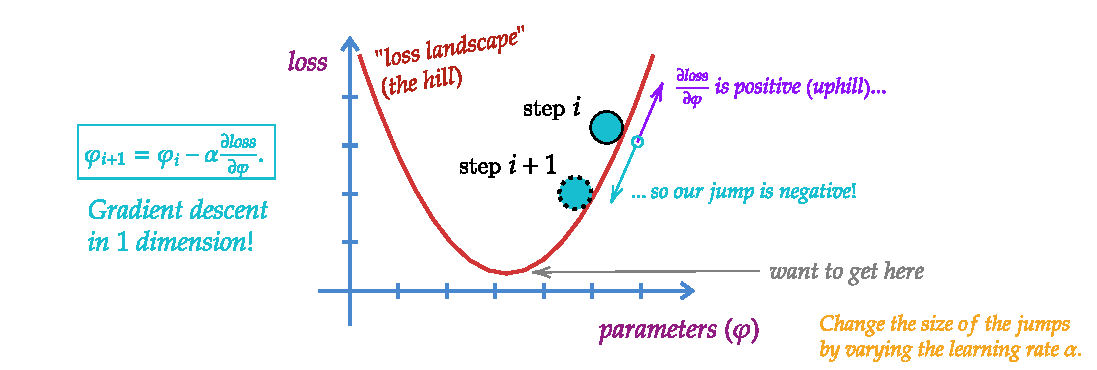
\includegraphics{./images/gdesc3.pdf}

}

\caption{\label{fig-ball-rolling}Gradient descent is more easily
digestible when considering it as rolling a ball down a hill, but you
need to play the role of gravity.}

\end{figure}

We're now specifying the data \(d\) because we want to give meaning to
the vertical position in the hill: it's some quantity that's assessing
the quality of our workflow with respect to some data from the real
world \(d\), given that we're using parameters \(\varphi_i\). In
practice this may be a small subset of the dataset that we draw at
random, since we can't computationally do this update on the whole data
set due to memory restrictions on the device we run this on.

A key point to highlight: this mechanism only works if \(L\) is
differentiable with respect to \(\varphi\), otherwise we won't be able
to calculate its gradient. This restriction may look tame for common
objectives, which tend to involve simple algebraic expressions involving
the output of a neural network, which is already a differentiable
function. However, if we want to add domain knowledge to our loss
function, we may end up discovering that not everything we want to
calculate has a well-defined gradient. There are various ways to get
around this, including the use of surrogate operations that are
\textbf{relaxed} (jargon for differentiable) versions of their
non-differentiable counterparts. We'll look at this in more detail when
we study applications of this nature.

Let's look at an example of gradient descent in action.

\hypertarget{example-maximum-likelihood-estimation}{%
\subsection{Example: maximum likelihood
estimation}\label{example-maximum-likelihood-estimation}}

Say we have some example data drawn from a bi-modal probability
distribution that's somewhat normal-looking, like in
Figure~\ref{fig-bidata}. We may want to try and model this with a normal
distribution, but how do we choose the parameters? We can fit them to
the data using maximum likelihood estimation, discussed further in
Section~\ref{sec-mle}. The basic idea is that, given a probability
distribution \(p\) with parameters \(\mu\), we want to calculate
\[ \hat{\mu} = \underset{\mu}{\mathrm{argmin}} (-2\ln p(x|\mu))~,\]

given some observed data \(x\). In other words, we want to find the
value of \(\mu\) such that we minimize the negative log-likelihood. We
can do this via gradient descent!

Using the update rule in Equation~\ref{eq-grad-descent} with \(L\) as
the negative log-likelihood and \((\mu, \sigma)\) playing the role of
\(\varphi\), we can run gradient descent for some number of steps until
we reach a result that converges within some tolerance. We'll have to
pick some initial value to start for each parameter -- here we use 1 for
each. In the implementation, we're using the automatic differentiation
framework JAX (Bradbury et al. (2018)) to calculate the gradient of the
objective (online viewers can expand the code block above the figure to
see the details). This gives us a result in Figure~\ref{fig-onenorm},
which isn't particularly great in my opinion.

\begin{figure}

{\centering 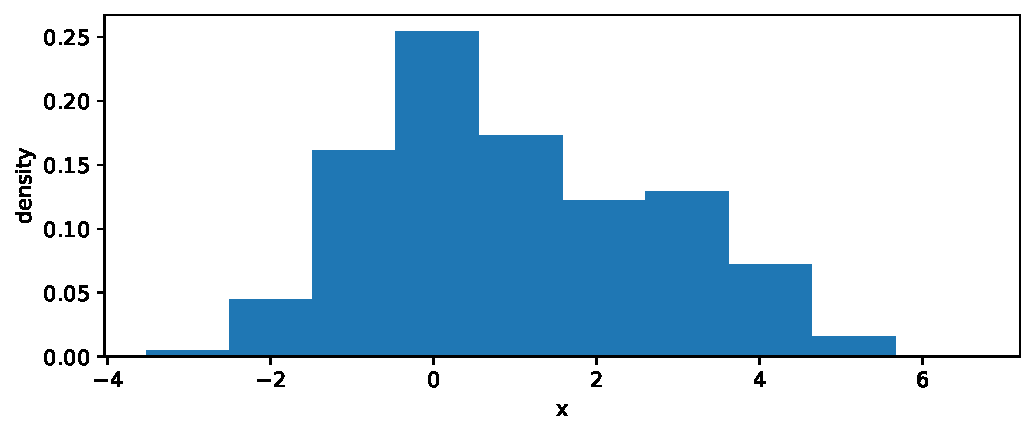
\includegraphics{./diffprog_files/figure-pdf/fig-bidata-output-1.pdf}

}

\caption{\label{fig-bidata}Example data produced using two normal
distributions in unequal amounts. One is centered on 3, and the other on
0, both with unit standard deviation.}

\end{figure}

\begin{figure}

{\centering 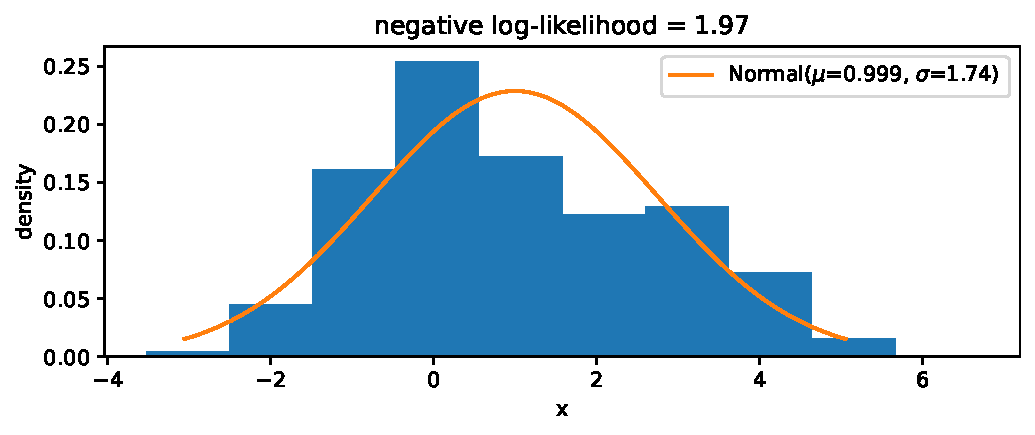
\includegraphics{./diffprog_files/figure-pdf/fig-onenorm-output-1.pdf}

}

\caption{\label{fig-onenorm}A single normal distribution fitted to the
data in Figure~\ref{fig-bidata} using gradient descent.}

\end{figure}

Pretending we didn't know that the data came from a mixture of normal
distributions, we can make a more sophisticated model, e.g.

\[
p(x |\mu_1, \sigma_1, \mu_2, \sigma_2) = \frac{1}{2}\mathrm{Normal}(\mu_1, \sigma_1) + \frac{1}{2}\mathrm{Normal}(\mu_2, \sigma_2)~.
\]

We can then simultaneously optimize \(\mu_1, \sigma_1, \mu_2, \sigma_2\)
in exactly the same way, with no modification to the procedure other
than using the new likelihood as the loss function. Doing this yields
the distribution in Figure~\ref{fig-twonorm}. We can tell that the shape
of the distribution is represented better here, which is also indicated
by the lower negative log-likelihood than in the case of the single
normal distribution. Since we forced the proportions of the mixture to
be half and half, the lower second peak is modelled through a wider
normal distribution to match the height of the second, smaller mode.

Interestingly, if we use 1 as the init for every parameter, we recover
the solution from Figure~\ref{fig-onenorm}, so we have to make sure
there's a little mutual variation in the starting values so that the
gradients push the different \(\mu\) and \(\sigma\) values from
different positions, allowing the second mode to be discovered. This
demonstrates the behavior of gradient descent to move to some
\emph{local} minimum of the objective, and won't always converge to
something optimal or intuitive.

\begin{figure}

{\centering 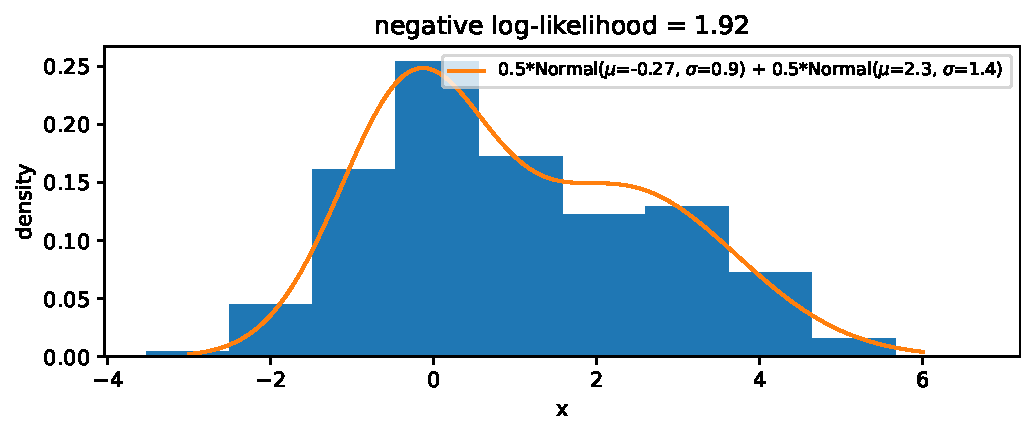
\includegraphics{./diffprog_files/figure-pdf/fig-twonorm-output-1.pdf}

}

\caption{\label{fig-twonorm}A mixture of two normal distributions fitted
to the data in Figure~\ref{fig-bidata} using gradient descent.}

\end{figure}

\hypertarget{mini-batching-and-stochastic-gradients}{%
\section{Mini-batching and stochastic
gradients}\label{mini-batching-and-stochastic-gradients}}

In reality, we're not generally able to update our parameters using
gradients computed over all our data at once in one batch, since that
data may not fit on the device we're using to compute the program. We'd
like to do this if we truly want to calculate the expectation of the
gradient (in practice, the empirical mean) across all the training data
we have, which has some convergence guarantees for arriving at a local
minimum. Instead, we often split our data up into \textbf{minibatches},
which are fixed-size partitions of the data, typically randomly
selected\footnote{There's a funny issue to do with the notion of
  randomly selecting here; if we select \emph{with replacement}, then
  we're sampling i.i.d. uniform random variables. This makes the theory
  of analyzing the performance much neater. But in practice, we never do
  this, and just shuffle the data and stream it, making it non-i.i.d,
  and therefore more difficult to analyze.}. When we have seen enough
batches such that we cover all the available training data, that number
of steps is known as an \textbf{epoch}. This gives rise to the notion of
the \textbf{batch size} -- the size of each partition -- which then
inherently decides how many steps an epoch will take (smaller batch size
= more steps and vice-versa).

An extreme version of splitting up into batches is \textbf{stochastic
gradient descent}, which is just setting the batch size to 1. Gradients
computed in this way will have very high variance as the name suggests,
since parameter updates would be based on the performance on each
individual training example. Surprisingly though, this high variance of
the gradients can often help when wanting to explore the loss landscape
more, and may help in jumping to new local minima that batch gradient
descent may ignore.

\hypertarget{speeding-up-convergence-different-optimizer-types}{%
\section{Speeding up convergence: different optimizer
types}\label{speeding-up-convergence-different-optimizer-types}}

To improve upon the rate of convergence in minibatch gradient descent,
several variants have been proposed that incorporate additional
information to make the gradient update. The methods are generally
referred to as \textbf{optimizers} -- we'll cover just a couple of the
more common ones here.

\hypertarget{momentum}{%
\subsection{Momentum}\label{momentum}}

What happens when we're in a ravine during optimization, i.e.~a local
minimum with two steep slopes on either side in one dimension? Without
modification, gradient descent will typically bounce between the
ravines: we're moving in the downward direction, and with a larger step
size since the slope is steep. How may we help this converge easier?
Well, we could of course modify the learning rate in an adaptive fashion
to try to dampen this oscillation about a minimum in a ravine. Something
else that is done is to incorporate some amount (\(\gamma\)) of the
\emph{previous update step}, which we can write with a modified update
rule through a placeholder variable \(v\), defined recursively:

\[
v_{i} = \gamma v_{i-1} + \alpha \frac{\partial L(\varphi_i, d)}{\partial \varphi_i};~~~ \varphi_{i+1} = \varphi_i - v_i~.
\]

To give some intuition as to what's happening here, we note that there's
still a standard gradient update rule in there, but we're also
``speeding up'' the update by an amount \(\gamma v_{i-1}\), meaning if
we did a large update previously, then we'll go even further this time.
The analogy here is really still a ball rolling down a hill, but we're
compounding speed just like gravity would make us do in real life.
Moreover, if the previous update had a different sign for the gradient
(travelling in the opposite direction), we'll actually be \emph{slowed}
by \(\gamma v_{i-1}\), which will prevent these types of oscillating
situations bouncing between two steep slopes. This is termed gradient
descent with \textbf{momentum}; I don't know if this was where it was
originally proposed, but many seem to cite (Qian 1999), despite it
opening with ``A momentum term is usually used in\ldots{}''.

\hypertarget{adagrad}{%
\subsection{Adagrad}\label{adagrad}}

We return to the idea of \emph{adaptive learning rates}. In the
multi-dimensional parameter setting (could even be billions if we're
looking at neural networks), some parameters will have higher importance
than others, i.e.~the loss landscape could be flat in some dimensions,
and convex in others. However, there could be parameters that are
locally flat in some region, but have more interesting structure at a
distance far from that region, or perhaps at least have structure that
is more widely spread out. This could happen if that parameter is
responsible for information relating to a sparse feature, for instance.
If the learning rate makes the stepsize small in comparison to this
distance, then we'll never explore that structure well. This then gives
rise to the notion of adapting the learning rate on a per-parameter
basis to aid more efficient exploration of the loss landscape in search
of a local minimum.

Adagrad (shorthand for ``adaptive gradient'') is a method that endeavors
to tackle this issue. It scales the learning rate for each parameter in
such a way as to increase the step size for parameters in which we have
moved less, and decrease it for those in which we have moved more.
Specifically, it scales the learning rate by the inverse of the sum of
the (squared) gradients. Denoting the gradient of one example parameter
\(\varphi^{(1)}\) at step \(i\) as \(g^{(1)}_{i}\), we can write the
update step for that parameter as

\[
\varphi^{(1)}_{i+1} = \varphi^{(1)}_{i} + \Delta\varphi_i^{(1)};~~~ \Delta\varphi_{i}^{(1)} = - \frac{\alpha}{\sqrt{\sum^{i}_{j=0}\left(g^{(1)}_{j}\right)^2 + \epsilon}} g^{(1)}_{i} ~,
\]

where \(\epsilon\) is a very small number just to prevent dividing by
zero. We've defined the convenient notation of \(\Delta\varphi\), which
becomes the subject of modification for the methods hereafter. For \(n\)
parameters, we denote \(g_{i}\) as the vector of all gradients
\([g^{(1)}_{i}, \dots, g^{(n)}_{i}]\). Then, if we treat all the
operations as \emph{elementwise}, i.e.~as one may expect with
\texttt{numpy} arrays, we can write this again more compactly for all
parameters \(\varphi\) as

\[
\varphi_{i+1} = \varphi_{i} + \Delta \varphi_i ;~~~ \Delta\varphi_i = - \frac{\alpha}{\sqrt{\sum^{i}_{j=0}g^2_{j} + \epsilon}} g_{i} ~.
\]

One of the main reasons for the appeal in Adagrad is that you don't
really need to tune the scalar learning rate \(\alpha\) from it's
initial value, since it's being done on-the-fly for each parameter.
However, an issue arises in that the sum \(\sum^{i}_{j=0}g^2_{j}\) is
one of positive numbers, and shall grow without bound, which will
eventually reduce the learning rate to a crawl and stop learning
altogether. Avoiding this is the groundwork for our next optimizers:
Adadelta and RMSProp.

\hypertarget{adadeltarmsprop}{%
\subsection{Adadelta/RMSProp}\label{adadeltarmsprop}}

As mentioned, tackling the growing sum of squared gradients is the
purpose behind Adadelta (Zeiler 2012) and RMSProp (Hinton 2018), where
we'll start with the former.

Instead of maintaining a sum over the gradients \(g_i^2\) up to step
\(i\), we recursively define a \emph{decaying average}
\(E\left[g^2\right]_i\):

\[
E\left[g^2\right]_i=\gamma E\left[g^2\right]_{i-1}+(1-\gamma) g_i^2~,
\]

where we proportionally weight the previous average and the current
squared gradient, each by a factor of \(\gamma\) and \(1-\gamma\)
respectively. This is a similar idea to momentum: we're ``remembering''
the previous steps in some manner that we can tune numerically through
\(\gamma\). This leads to a \(\Delta \varphi_i\) of

\begin{equation}\protect\hypertarget{eq-adadelta1}{}{
\Delta \varphi_i = - \frac{\alpha}{\sqrt{E\left[g^2\right]_i+ \epsilon}} g_{i} ~.
}\label{eq-adadelta1}\end{equation}

Coincidentally, this is actually the equation for the \emph{RMSProp}
update, developed independently from Adadelta around the same time! For
Adadelta though, we're not quite done yet though; the Adadelta authors
noted that this update of \(\Delta \varphi_i\) -- just like the update
in \emph{any} of the methods above -- does not have the same units as
the parameters (it's instead dimensionless), which is not in principle
an issue, but maybe better behaviour could be had by updating by a
quantity of the same scale as the parameters themselves. This led to
defining a second decaying average using the definition of
Equation~\ref{eq-adadelta1} for \(\Delta \varphi_i\), which we'll also
define recursively:

\[
E\left[\Delta \varphi^2\right]_i=\gamma E\left[\Delta \varphi^2\right]_{i-1}+(1-\gamma) \Delta \varphi_i^2 ~.
\]

This expression is then also put under a square root with the same small
\(\epsilon\), and we use this in place of the static learning rate
\(\alpha\), i.e.~replace it with
\(\sqrt{E\left[\Delta \varphi^2\right]_i + \epsilon}\). At least, we'd
like to -- this would lead to some kind of nested recursion relation
between \(E\left[\Delta \varphi^2\right]_i\) and \(\Delta \varphi_i\),
so we need to instead need to approximate this with a value we have
access to. The paper does this with the value from the previous
iteration: \(E\left[\Delta \varphi^2\right]_{i-1}\). This at last gives
us the full relation for one Adadelta update:

\begin{equation}\protect\hypertarget{eq-adadelta}{}{
\Delta \varphi_i = - \frac{\sqrt{E\left[\Delta \varphi^2\right]_{i-1} + \epsilon}}{\sqrt{E\left[g^2\right]_i+ \epsilon}} g_{i} ~.
}\label{eq-adadelta}\end{equation}

A curious thing to note in Equation~\ref{eq-adadelta} is the lack of
\(\alpha\) -- we've removed the scalar learning rate altogether, and
instead only need to specify the decay factor \(\gamma\) before
undergoing optimization.

\hypertarget{adam}{%
\subsection{Adam}\label{adam}}

We've reached \textbf{Adam} (Kingma and Ba 2014): by far the most common
default choice of optimizer for deep learning, and the one frequently
used within this thesis. Adam draws upon ideas from all of the above
methods; it keeps track of both a decaying average of gradients
\emph{and} squared gradients. We can write their forms explicitly:

\[
\begin{aligned}
m_i &=\beta_1 m_{i-1}+\left(1-\beta_1\right) g_i \\
v_i &=\beta_2 v_{i-1}+\left(1-\beta_2\right) g_i^2~,
\end{aligned}
\] where we've introduced separate decay factors \(\beta_1\) and
\(\beta_2\) for each quantity. If you remember earlier, we were using
\(E[g]_i\) notation for these types of quantities, and that's not a
coincidence -- they're moving averages, and so are Monte Carlo
estimations of expectation values (albeit off by decay terms etc).
Specifically, \(m_i\) and \(v_i\) are estimators of the first moment
(mean) and second moment (variance) of the gradients \(g_i\), hence
their variable names, and the name of Adam (adaptive \emph{moment}
estimation).

One thing the Adam authors note is the fact that they used the algorithm
through initializing \(m_i\) and \(v_i\) as vectors of zeroes, and then
found that the resulting estimates of the gradient moments were biased
towards zero. The paper includes a brief derivation of the actual value
of these moments, and shows that in either case of \(m_i\) or \(v_i\),
you can correct for this bias by dividing through by \((1-\beta^i)\),
where we explicitly raise \(\beta\) to the power of the iteration number
\(i\) (the paper uses \(t\) instead). This results in the bias-corrected
version of the previous formula: \[
\begin{aligned}
\hat{m}_i &=\frac{m_i}{1-\beta_1^i} \\
\hat{v}_i &=\frac{v_i}{1-\beta_2^i}~.
\end{aligned}
\] We then use these bias-corrected moment estimates to construct an
expression for the Adam update, which looks a lot like that for RMSProp
in Equation~\ref{eq-adadelta1}:

\[
\Delta \varphi_i = - \frac{\alpha}{\sqrt{\hat{v}_i}+ \epsilon} \hat{m}_{i} ~.
\]

As you can see, gradient descent can get pretty complicated! The reason
I went through this explicitly was to show that gradient descent has
been extremely well-studied during the rise of deep learning, and we
often need to go beyond simple update rules in order to effectively
learn the properties we want from our parameters in practice. In fact,
the main work you'll see in the first application later on initially
wouldn't learn at all until we switched to using Adam!

\subsection{A quick comment on ``local'' minima}

I've painted a picture of very nice, well-behaved hills that have clearly defined bottoms. Clearly if we need all the machinery with optimizer modifications, there's probably a rougher situation in reality.

If you think about neural networks -- the clear majority usage of gradient descent in practice -- the loss landscape can have dimensionality in the millions/billions/trillions, since every parameter introduces a new axis. When we talk about the ``optimum'' solution, then, we're really only ever going to arrive at some \textit{local} minimum of the loss function, which may or may not be the level of performance we desire for our given task. This is partially why the act of training may different networks with different initializations for the weights and averaging the results (called \textit{ensembling}) is so common, as you'll likely have many unique minima in your loss landscape that carry different levels of performance; combining them can then help cover possible failure modes of any particular choice of minimum, and also gives you some measure of uncertainty.

So: this was a birds eye view on gradient descent, which is by-and-large the way machines learn. It's very humbling to realize that this fairly simple idea is underpinning so much of the modern world around us, and will only continue to do so.

\hypertarget{automatic-differentiation}{%
\chapter{Automatic differentiation}\label{automatic-differentiation}}

One may think that the pace of scientific discovery is determined by the
speed at which new ideas are formed. That was likely true in the early
days; if I posited that a rock, when thrown, will roughly trace a
parabolic arc, we likely don't need to take leaps in experimental
physics to test this hypothesis to some ballpark degree of accuracy --
maybe we could even get away with just a ruler and the naked eye. In
contrast to this, science as done in the present requires a little
additional technology in order to probe the questions that we're
interested in (unless we get really, really good rulers).

I say this to emphasize that the advancements made in deep learning over
the past couple decades can be largely attributed to the ability to run
\emph{efficient and exact} learning algorithms at scale. For this, we
have \textbf{automatic differentiation} to thank (which we playfully
term ``autodiff''), which allows us to take the gradient of pretty much
arbitrary computer code. Which is pretty damn cool.

This section will take a tour through the basics of gradient
computation, and then we'll compare the different types of automatic
differentiation mechanisms (do we build a graph of our program before
executing the code, or do we trace it at runtime?), and then show some
example code for each.

\hypertarget{building-blocks-of-automatic-differentiation}{%
\section{Building blocks of automatic
differentiation}\label{building-blocks-of-automatic-differentiation}}

The core idea of autodiff is the breaking down of a potentially
complicated calculation into a set of computational \textbf{primitives}:
basic operations with known derivatives. Think of things like \(+\),
\(\times\), \(-\), \(\div\), \(\sin\), \(\log\), and so on. We know how
to take the derivative across each of these operations analytically, so
we can say to a computer ``Every time you see a \(\sin\), replace it
with a \(\cos\) in the gradient calculation''. Then, thanks to the chain
rule, we can build up the gradient of the whole program by multiplying
these gradient results together.

Getting into the specifics of this, we'll begin by focusing on a
function \(F: \mathbb{R}^n \rightarrow \mathbb{R}\), which is a scalar
valued function that takes in a vector input of dimensionality \(n\),
and returns a scalar. We deliberately choose this to mimic an objective
function as seen in deep learning, which typically maps a
high-dimensional vector of weights \& biases to a single real number. We
can also explicitly denote the application and output of \(F\) as
\(F(\mathbf{x}\in\mathbb{R}^n) \rightarrow y \in \mathbb{R}\).

If we break down \(F\) into a composition of (arbitrarily) four other
functions, we would write that as \(F = D \circ C \circ B \circ A\).
Each one of these can be any random operation, like adding 5, taking the
logarithm, or hooking into your OS to gain \texttt{root} access
(equivalent to the identity operation from a numerical perspective). We
can write this explicit chain of computations as
\(y = F(\mathbf{x}) = D(C(B(A(\mathbf{x}))))\), where we can interpret
the computation as starting from the inner level, i.e.~application of
\(A\) to \(\mathbf{x}\), then \(B\) to \(\mathbf{a} =\) the output of
\(A(\mathbf{x})\)), and so on. Let's also define
\(\mathbf{b} = B(\mathbf{a})\), \(\mathbf{c} = C(\mathbf{b})\), and
\(y = D(\mathbf{c})\).

We'll see why function composition is important to cover -- a core idea
of automatic differentiation is to break down the gradient of the whole
into the composition of the gradient of its parts via the chain rule.
But more on that later.

Let's turn to gradients: we define the \textbf{Jacobian matrix} of
partial derivatives of \(F\) as

\begin{equation}\protect\hypertarget{eq-jacobian}{}{
J_F(\mathbf{x}) = F'(\mathbf{x}) = \left[\begin{array}{ccc}\frac{\partial y_{1}}{\partial x_{1}} & \cdots & \frac{\partial y_{1}}{\partial x_{n}} \\\vdots & \ddots & \vdots \\\frac{\partial y_{m}}{\partial x_{1}} & \cdots & \frac{\partial y_{m}}{\partial x_{n}}\end{array}\right],
}\label{eq-jacobian}\end{equation}

assuming \(y\) has multiple components (\(y_1\), \(y_2\), etc.).
However, since we're going from \(\mathbb{R}^n \rightarrow \mathbb{R}\),
the Jacobian is just one row vector:

\[
F'(\mathbf{x}) =  \left[ \frac{\partial y}{\partial x_1} , \frac{\partial y}{\partial x_2}, \cdots, \frac{\partial y}{\partial x_n}\right].
\]

Given the decomposition of \(F\) above, we can break this down into a
product of individual Jacobian matrices for each of the intermediate
functions via the chain rule:

\[
F'(\mathbf{x}) = \frac{\partial y}{\partial \mathbf{c}}\frac{\partial \mathbf{c}}{\partial \mathbf{b}}\frac{\partial \mathbf{b}}{\partial \mathbf{a}} \frac{\partial \mathbf{a}}{\partial \mathbf{x}},
\]

One can note the sizes of each of the intermediate matrices in the
format (\# rows, \# columns):

\begin{align*}
\mathrm{size}(\partial y / \partial \mathbf{c}) &= (1,\mathrm{len}(c)) \\
\mathrm{size}(\partial \mathbf{c} / \partial \mathbf{b} ) &= (\mathrm{len}(c), \mathrm{len}(b)) \\
\mathrm{size}(\partial \mathbf{b} / \partial \mathbf{a} ) &= (\mathrm{len}(b), \mathrm{len}(a)) \\
\mathrm{size}(\partial \mathbf{a} / \partial \mathbf{x} ) &= (\mathrm{len}(a), n)~,
\end{align*}

where $\mathrm{len}(x)$ is the size of the leading dimension for the vector $x$.

The size of the final Jacobian matrix is then \((1, n)\), as shown
earlier (i.e.~one row vector). We'll come back to why these sizes are
important -- for instance, these matrices could be very hard to store
if \(n\) is large.

This kind of sequential matrix multiplication can be called
``accumulating'' the Jacobian piece-by-piece. The order of the
multiplication of these matrices (i.e.~where to put the parentheses)
matters to optimize computational load, but we'll look at two particular
extreme cases:

\begin{itemize}
\tightlist
\item
  \textbf{Forward accumulation}: Start from the input and work forwards
  to the output (right to left)
\end{itemize}

\[
F'(\mathbf{x}) = \frac{\partial y}{\partial \mathbf{c}}\left(\frac{\partial \mathbf{c}}{\partial \mathbf{b}}\left(\frac{\partial \mathbf{b}}{\partial \mathbf{a}} \cdot \frac{\partial \mathbf{a}}{\partial \mathbf{x}}\right)\right),
\]

Here's an example of what that first matrix product looks like: \[
\frac{\partial \mathbf{b}}{\partial \mathbf{a}} \cdot \frac{\partial \mathbf{a}}{\partial \mathbf{x}}\ =\frac{\partial \mathbf{b}}{\partial \mathbf{x}}=\left[\begin{array}{ccc}\frac{\partial b_{1}}{\partial x_{1}} & \cdots & \frac{\partial b_{1}}{\partial x_{n}} \\\vdots & \ddots & \vdots \\\frac{\partial b_{m}}{\partial x_{1}} & \cdots & \frac{\partial b_{m}}{\partial x_{n}}\end{array}\right].
\]

\begin{itemize}
\tightlist
\item
  \textbf{Reverse accumulation}: vice-versa!
\end{itemize}

\[
F'(\mathbf{x}) = \left( \left( \frac{\partial y}{\partial \mathbf{c}} \cdot \frac{\partial \mathbf{c}}{\partial \mathbf{b}} \right)\frac{\partial \mathbf{b}}{\partial \mathbf{a}} \right)\frac{\partial \mathbf{a}}{\partial \mathbf{x}},
\]

Again, let's take a look at the result of the first matrix product:

\[
\frac{\partial y}{\partial \mathbf{c}} \cdot \frac{\partial \mathbf{c}}{\partial \mathbf{b}}\ =\frac{\partial y}{\partial \mathbf{b}}= \left[ \frac{\partial y}{\partial b_1} , \frac{\partial y}{\partial b_2}, \cdots, \frac{\partial y}{\partial b_n}\right]
\]

Why is that so much smaller than forward accumulation? Our initial
matrix \(\partial y / \partial \mathbf{c}\) has only one row due to
\(y\) being 1-dimensional. Moreover, we note that this causes the size
of every intermediate matrix product to always be \((1, \dots)\),
meaning if we have this situation where we're going from
\(\mathbb{R}^n \rightarrow \mathbb{R}\) like with \(F\), reverse
accumulation looks much more efficient in terms of memory usage and
compute to get the same result, since we're only ever storing
intermediate vectors and not high-dimensional matrices. This is the
typical setting with a neural network: we have a very large input space
(could even be \textasciitilde billions of parameters), and we want to
evaluate the Jacobian matrix of a scalar (which would have one row and
\textasciitilde billions of columns) with respect to those parameters.
If we had the complementary setting,
i.e.~\(\mathbb{R} \rightarrow \mathbb{R}^n\), which could maybe be some
parametrization of a simulator that produces high-dimensional data, we
would probably want to compute the Jacobian with forward-mode
accumulation instead.

\hypertarget{jacobian-vectorvector-jacobian-products}{%
\subsection{Jacobian-vector/vector-Jacobian
products}\label{jacobian-vectorvector-jacobian-products}}

Let's touch again on this idea of only storing intermediate vectors: we
can see this arose in the case of reverse accumulation from the fact
that our first multiplication had a 1 in the external dimensions,
i.e.~was a \emph{row} vector \(\mathbf{v}^T\) multiplying from the left.
We can recover this situation for forward mode if we pre-multiply the
Jacobian matrix by some \emph{column} vector \(\mathbf{v}\) from the
right. This leads us to think about the generality offered by
considering Jacobian-vector and vector-Jacobian products (JVP/VJPs) as
primary functions of forward and reverse mode autodiff respectively.

To illustrate this with equations, we can write a JVP for our function
\(F\) with the same operation ordering as with the \emph{forward}
accumulation of a Jacobian:

\[
F'(\mathbf{x})\,\mathbf{v} = \frac{\partial y}{\partial \mathbf{c}}\left(\frac{\partial \mathbf{c}}{\partial \mathbf{b}}\left(\frac{\partial \mathbf{b}}{\partial \mathbf{a}} \left(\frac{\partial \mathbf{a}}{\partial \mathbf{x}} \mathbf{v} \right) \right)\right)
\]

Thinking of the rules of matrix multiplication, we note that
\(\frac{\partial \mathbf{a}}{\partial \mathbf{x}} \mathbf{v}\) is only
tractable if \(\mathbf{v}\) is of size \texttt{(n,\ 1)}, since
\(\frac{\partial \mathbf{a}}{\partial \mathbf{x}}\) is of size
\texttt{(len(a),\ n)}. Provided this is the case, all following
computations will include 1 as one of the outer dimensions, meaning we
once again only need to consider intermediary vectors instead of
matrices when computing this quantity.

Now, you may be thinking ``Nathan, this is all well and good, but what
\emph{is} the vector \(\mathbf{v}\), and why are you showing it to me?
Aren't we interested in the Jacobian itself, and not its product with
some arbitrary vector?''

Firstly, I would respond by asking why you're saying this in a thick
cockney accent. After that, I would then go on to say that we can still
use this formulation to recover the whole Jacobian -- we can simply let
\(\mathbf{v}\) be a \emph{one-hot encoding} (or \emph{unit vector} if
you're more mathematically inclined) of one of the input dimensions,
e.g.~\(\mathbf{v} = [1, 0, \dots, 0]^T\), and the result of our JVP will
then be the first \emph{column} of the Jacobian:

\begin{align}
    F'(\mathbf{x})\,\mathbf{v} &= \begin{bmatrix}
            \frac{\partial y_1}{\partial x_1} \\
            \frac{\partial y_2}{\partial x_1}\\
            \vdots
        \end{bmatrix}
\end{align}

We can repeat this for each dimension by changing the place we put the 1
in \(\mathbf{v}\), then concatenate the results to get the whole
Jacobian. So by building up the Jacobian one column at a time when doing
forward accumulation, we gain this advantage we talked about earlier of
only storing intermediate vectors, and never having to instantiate any
potentially large matrices, regardless of the dimensionality of the
input or output.

Ah, but wait a minute, I used \(y_1, y_2\) etc. above -- my mistake, we
don't actually have a vector for our choice of \(F\) from earlier. We
only have just one scalar output \(y\). That means that the result of
our computation above would be the single first element of the Jacobian:
\(\partial y / \partial x_1\), and we would need one JVP calculation for
each element. That seems a bit excessive! Wasn't reverse mode meant to
be better? Shouldn't we use that?

Agreed. Let's do the same thing, and produce a \emph{vector-Jacobian
product} with a one-hot encoding of the output dimensions.

\begin{align}
\mathbf{v}^T \, F'(\mathbf{x}) &= \left( \left( \left( \mathbf{v}^T \,\frac{\partial y}{\partial \mathbf{c}} \right) \frac{\partial \mathbf{c}}{\partial \mathbf{b}} \right)\frac{\partial \mathbf{b}}{\partial \mathbf{a}} \right)\frac{\partial \mathbf{a}}{\partial \mathbf{x}} \\
& =\left[ \frac{\partial y_1}{\partial x_1} , \frac{\partial y_1}{\partial x_2}, \cdots, \frac{\partial y_1}{\partial x_n}\right].
\end{align}

We've calculated the first \emph{row} of the Jacobian, and can construct
the full thing with a VJP for each row, corresponding to each dimension
of the output. In the case of this output \(y\) being scalar as before,
that would make \(\mathbf{v}^T = 1\) (only one output dimension), and we
recover the full Jacobian in one go, since it was only one row to begin
with! But of course, if \(y\) had multiple dimensions (say 5), we would
only have to compute 5 VJPs to form the whole Jacobian, never having to
worry about the size of the intermediate quantities.

Based on these appealing properties, it helps when using autodiff to
consider the JVP/VJP as the fundamental operation when calculating
gradients of programs in practice. It's a funny way of thinking at
first, but the quantity we end up with is just the regular Jacobian (or
elements thereof) in the end, so it's only important when considering
implementation details of gradient computations.

To summarize: we've seen the difference between \textbf{forward}- and
\textbf{reverse}-mode autodiff, and their usefulness in constructing
Jacobians via \textbf{Jacobian-vector} and \textbf{vector-Jacobian
products}, which bypass the need to store large intermediate matrices
by forming the Jacobian one column or one row at a time respectively. We
also note that for the deep learning case of interest, where we have an
objective function \(F\) that maps
\(\mathbb{R}^n \rightarrow \mathbb{R}\) with \(n\) large, we far prefer
\emph{reverse-mode} autodiff to calculate its gradient, which we need to
perform optimization.

\hypertarget{from-sequences-to-graphs}{%
\subsection{From sequences to graphs}\label{from-sequences-to-graphs}}

One thing that you may have noticed in our previous section is the fact
that we focused only on a simple decomposition of \(F\) into the
sequential application of four functions \(A\), \(B\), \(C\), and \(D\)
to the input \(\mathbf{x}\). In reality, computer programs are going to
look a lot more complicated, and will be represented by the more general
construct of a directed acyclic graph (DAG). We need to adapt the above
framework for JVPs/VJPs in order to generalize to these real-life
scenarios.

It turns out this is fairly simple: we only need to consider two
additional cases than what we've considered already. The application of
a single operation with a single input and output would be represented
as one node in a graph, with an edge going in and coming out. Luckily,
the only additional generalization we need to consider is the case of
multiple inputs (fan-in) and multiple outputs (fan-out).

For the fan-in case, i.e.~multiple input values from different
computations: we know how to calculate Jacobians for a single input, so
we can just do this process for each input separately. More explicitly:
for \(F(\mathbf{a}, \mathbf{b})\), with \(\mathbf{a}\) and
\(\mathbf{b}\) possibly coming from different parts of the program, we
calculate the Jacobian for each input separately as before:
\(F'_\mathbf{a}(\mathbf{a}, \mathbf{b}) = \partial y / \partial \mathbf{a}\)
and
\(F'_\mathbf{b}(\mathbf{a}, \mathbf{b}) = \partial y /\partial \mathbf{b}\).

Fan-out is slightly more involved, since we now have the case of
multiple return values. Let's examine a function with this behaviour:
\(G(\mathbf{x}) = [3\mathbf{x}, 5\mathbf{x}]^T\). We can see that this
input replicates our input \(\mathbf{x}\) with different factors applied
to each output, which we can represent through the linear function
\(G(\mathbf{x}) = [3I, 5I]^T\mathbf{x}\), where \(I\) is the identity
matrix. The Jacobian of \(G\) is then just the coefficients multiplying
\(\mathbf{x}\): \(G'(\mathbf{x}) = [3I, 5I]^T\). But in practice, we're
probably going to be computing a VJP across this node in the graph
during backpropagation. Remembering that this involves multiplying by a
vector \(\mathbf{v}^T\) with the same dimensionality of the output of
\(G\), we can then write
\(\mathbf{v}^T = [\mathbf{v_1}^T, \mathbf{v_2}^T]\), one vector for each
vector in \(G(\mathbf{x})\). This then leads to

\begin{align}
\mathbf{v}^TG'(\mathbf{x})  &= [\mathbf{v_1}^T, \mathbf{v_2}^T][3I, 5I]^T \\
&= 3\mathbf{v_1}^T +  5\mathbf{v_2}^T.
\end{align}

So if we have a function with multiple outputs, we'll be accumulating
the VJP of that function across the outputs through addition. We can see
that this results from the shapes of the vectors being multiplied here,
which will always result in an outer shape of \texttt{(1,\ 1)}, so we
can safely generalize this to any number of outputs.

\begin{figure}

\begin{minipage}[t]{0.50\linewidth}

{\centering 

\raisebox{-\height}{

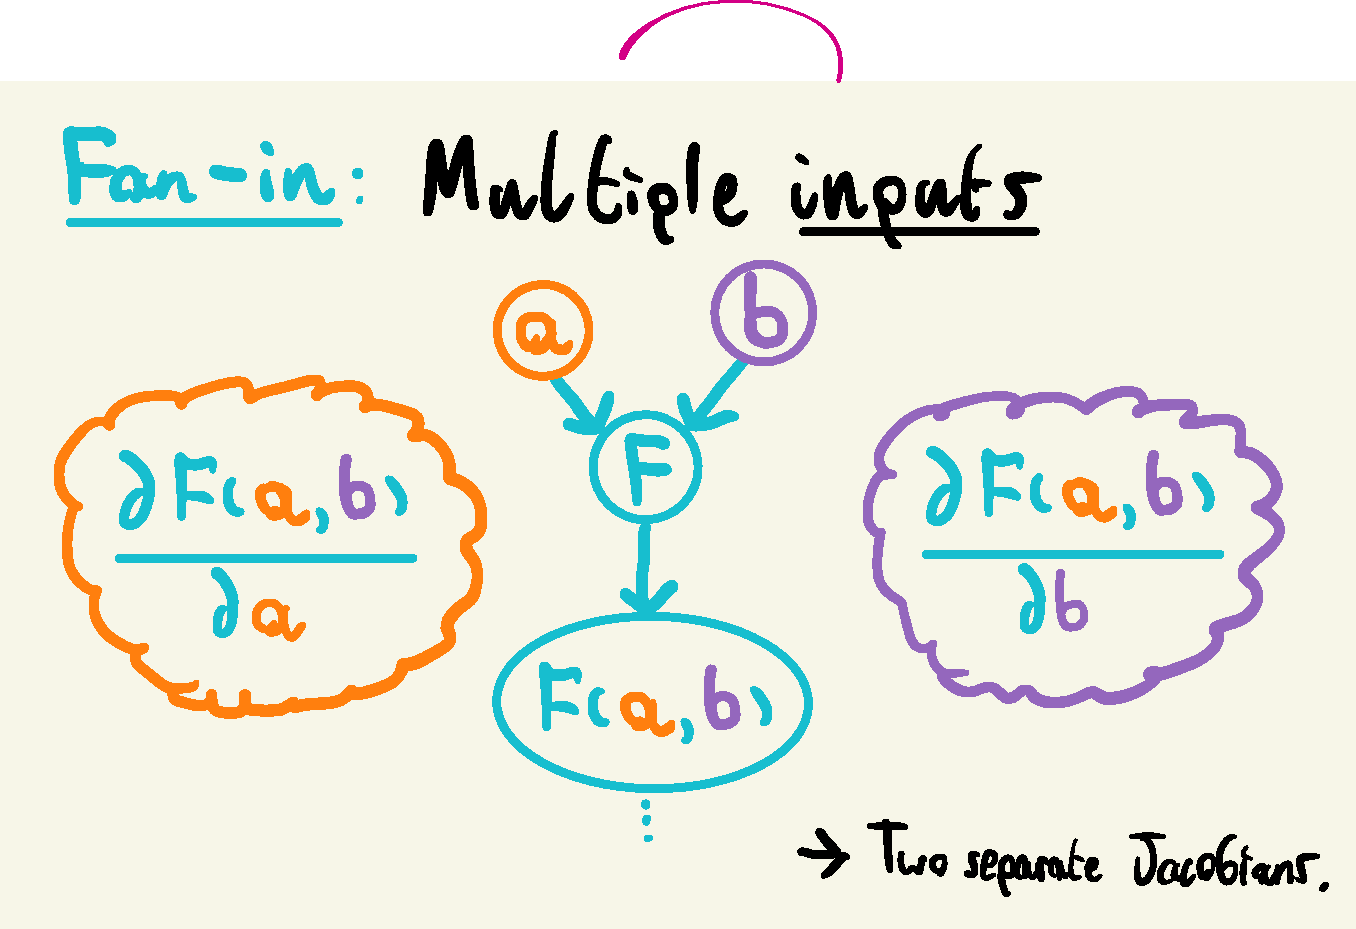
\includegraphics{./images/fanin.pdf}

}

}

\subcaption{\label{fig-fanin}Fan-in}
\end{minipage}%
%
\begin{minipage}[t]{0.50\linewidth}

{\centering 

\raisebox{-\height}{

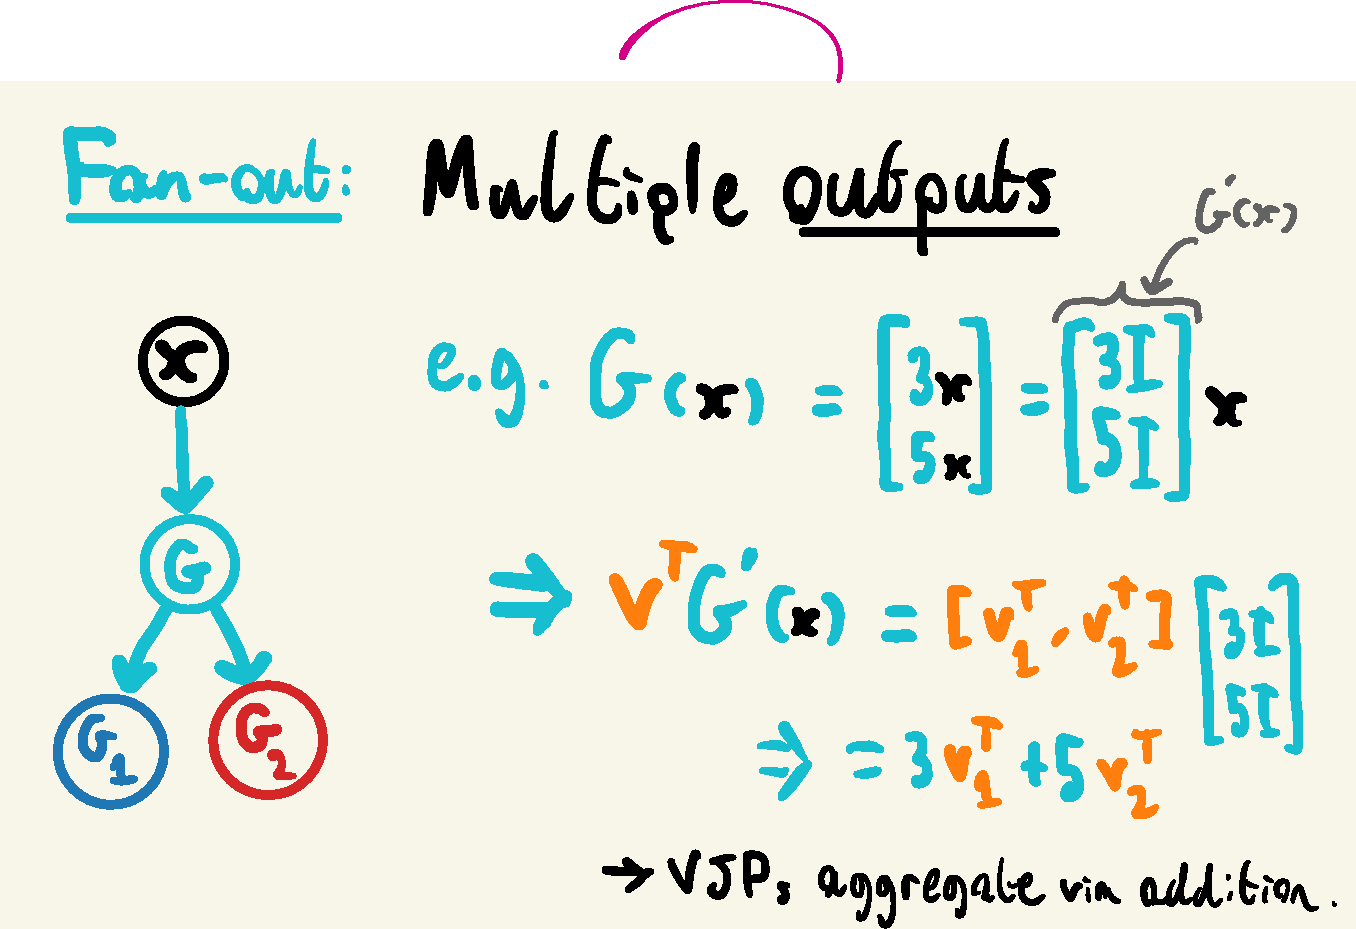
\includegraphics{./images/fanout.pdf}

}

}

\subcaption{\label{fig-fanout}Fan-out}
\end{minipage}%

\caption{\label{fig-fan}Demonstration of how functions that fan-in and
fan-out are handled when gradients are computed with respect to their
input(s). Somehow gained fun pink coathangers in the image-making process.}

\end{figure}

That's pretty much all the scaffolding we need in terms of a framework
to calculate gradients. The only missing pieces are:

\begin{itemize}
\tightlist
\item
  A way to express the program in a graph
\item
  An implementation of the vector-Jacobian and Jacobian-vector
  operations
\end{itemize}

We'll discuss both of these in the following sections.

\hypertarget{building-the-computation-graph}{%
\section{Building the computation
graph}\label{building-the-computation-graph}}

There are two main existing strategies to represent a series of code
computations as a graph. One involves letting the user build up the
graph structure manually via library-provided primitives -- called
\textbf{define-and-run}; the resulting construct is known as a
\emph{static graph}, and is the approach taken by libraries like
\href{https://github.com/Theano/Theano}{Theano} and
\href{https://github.com/google/tensorflow}{TensorFlow} (when run
without eager execution). This has the unfortunate side effect of making
code much more difficult to read and write, since you have to use
symbolic proxies for operations like control flow and looping
(e.g.~\texttt{tf.while\_loop} instead of Python's \texttt{while}) in
order to instantiate that operation in the graph.

The other approach, known as \textbf{define-by-run}, builds up a
\emph{dynamic graph} structure during a program's execution. How does
this work? The program is \emph{traced} at runtime, meaning that the
autodiff framework is watching which operations occur when a function is
run in order to build up the computation graph for that function. When
done this way, incorporating loops and conditional structure within the
graph is no longer needed: at runtime, loops are unrolled into
sequences, and the branching induced by conditional logic will collapse
to one branch when the program is actually ran. These properties make
define-by-run the more popular approach to autodiff, and is the approach
taken by libraries such as \href{https://github.com/google/jax}{JAX},
\href{https://github.com/pytorch/pytorch}{PyTorch}, and
\href{https://ai.googleblog.com/2017/10/eager-execution-imperative-define-by.html}{Tensorflow
(eager execution mode)}. It's worth noting that since evaluating the
gradients requires tracing the program, i.e.~evaluating the function,
the runtime cost for the gradient calculation is usually of the same
order as the program itself. Why? For each primitive in the program,
there's a corresponding step in the gradient computation (e.g.~wherever
you see a \(\log{x}\) in your program, there'll be a \(1/x\) somewhere
in the JVP/VJP call), so the computations are almost totally identical
in compute\footnote{This may not hold when you're doing fancy things
  like checkpointing, which I haven't covered here.}.

\hypertarget{sec-fixed-points}{%
\section{Differentiating fixed points}\label{sec-fixed-points}}

We spend a bit of time here on the more niche topic of differentiating a
fixed point, as we make use of this result later. A \textbf{fixed point}
\(x^*\) of a function \(f\) is defined by the relation

\[
f(x^*) = x^*,
\]

meaning if we apply \(f\) (even multiple times), we remain stationary at
the point we applied \(f\) to. Why is this of interest, i.e.~what kind
of functions of importance exhibit this behavior?

The first and easiest thing is of course the straight line \(f(x) = x\),
which has the whole real line as fixed points. But maybe we're more
interested in the case where the fixed point is a quantity of interest
-- this is the case for something like an \emph{optimization loop}.
Here's an example where \(f\) is one gradient descent step:

\begin{align}
&f(x, \mathrm{loss}) = x - \frac{\partial\, \mathrm{loss}}{\partial x}\left( \times \, \mathrm{learning~rate~etc.}\right)
\\ \Rightarrow &f(x^*, \mathrm{loss} ) = x^*;~~~x^* = \underset{x}{\mathrm{argmin}}\, \mathrm{loss}.
\end{align}

As above, if our gradient descent is any good, then we'll hopefully
converge to the fixed point \(x^*\), which is the value of \(x\) that
lies in some local minimum of the loss function. Further iterations will
then not do anything -- we'll still be sitting at \(x^*\). How might we
take the gradient of this fixed point? Moreover, what if this gradient
is with respect to parameters that implicitly define the loss itself?

The first thing to highlight is that in practice, we'd take many steps
to reach the minimum, which corresponds to many sequential applications
of \(f\) to some initial value of \(x\). In the framework of automatic
differentiation outlined in previous sections, this would mean taking
the gradient (in a define-by-run setting) would \emph{unroll} the
optimization loop at runtime, and decompose \emph{each} of these
per-iteration applications of \(f\) into their primitives, and compose
their vector-Jacobian products or similar. For an optimization loop,
this could involve thousands of steps! Moreover, all that work that
happens in the early stages of optimization far from the fixed point
\(x^*\) will likely not impact the gradient of the fixed point itself --
we're much more interested in the steps close to convergence.

To get around this computational issue, we can employ the use of the
\textbf{implicit function theorem}. The full details of the theorem are
beyond the scope of this application, but it guarantees some things that
we'll state here. To be consistent with later sections, we will now
switch symbols from \(x\) to \(\theta\) (which will denote parameters
we're optimizing), and include \(\varphi\) as parameters that
\emph{implicitly} define part of \(f\) (e.g.~that define the objective
function used in optimization).Now, for a different function
\(g(\theta, \varphi)\), where there exists some solution
\(g(\theta_0, \varphi_0) = 0\), then the following holds:

A \emph{solution mapping function} exists in the form of
\(\theta^*(\varphi)\) such that

\begin{itemize}
\tightlist
\item
  \(\theta^*(\varphi_0) = \theta_0\)
\item
  \(g(\theta^*(\varphi), \varphi) =0~~~\forall \varphi\)
\item
  \(\theta^*\) is \emph{differentiable} with respect to \(\varphi\)!
\end{itemize}

To put this into words: as long as there exists \emph{some} solution
that makes \(g(\theta, \varphi) = 0\), we get a mapping for the
\emph{general solution} as a function of \(\varphi\), which is
differentiable. This means that as long as we find a way to calculate
that gradient, we can directly access the gradients of the solution
\(\theta_0\) that we found during optimization with respect to the
particular \(\varphi_0\) that we used, all thanks to the general
function \(\theta^*\).

Now, notice that we wrote this holding for \(g(\theta, \varphi) = 0\),
which we don't have quite yet. But we can define this for our update
state \(f\) by simply letting
\(g(\theta, \varphi) = f(\theta, \varphi) - \theta\). Now, when we
arrive at our solution \(\theta_0\) as the fixed point of \(f\) for some
\(\varphi_0\), we'll get
\(g(\theta_0, \varphi_0) = \theta_0 - \theta_0 = 0\), and in turn have
access to all those nice properties! We just need to explicitly
calculate the gradient of \(\theta^*\) now, which we can do by
differentiating both sides of \(g(\theta^*(\varphi), \varphi) =0\):

\[
\frac{\partial g(\theta^*(\varphi), \varphi)}{\partial\varphi} = \frac{\partial g}{\partial \theta^*}\frac{\partial \theta^*}{\partial \varphi} + \frac{\partial g}{\partial\varphi}~.
\]

Then in practice, we'll have \(\theta_0\) as our optimization solution
and \(\varphi_0\) as our implicit parameters, which we can plug in, and
then rearrange for \(\partial\hat{\theta}/\partial\varphi\):

\[
    \frac{\partial\theta^*}{\partial\varphi} = \frac{\partial\theta_0}{\partial\varphi_0}= -\left[\frac{\partial g}{\partial \theta_0}\right]^{-1}  \frac{\partial g}{\partial \varphi_0} ~.
\]

Finally, we can substitute in our definition of \(g\) in terms of \(f\)
to get

\[
\frac{\partial\theta_0}{\partial\varphi_0}= \left[I - \frac{\partial f}{\partial \theta_0} \right]^{-1} \frac{\partial f}{\partial \varphi_0}~.
\] We've constructed an expression for the gradient of the fixed point
\(\theta_0\) of an update rule \(f\), and with respect to the parameters
\(\varphi\) that define the objective used in the optimization! This is
a fantastic result, as it means we can just use this expression instead
of unrolling the entire optimization loop itself, saving us lots of
memory and compute in the process.

To read more about this construction, and some of the finer details of
the implementation on the autodiff side (note how we skipped over the
conversation about the fact that we have VJPs and not gradients
directly), I would thoroughly recommend (Duvenaud, Johnson, and Kolter,
n.d.), which I based this section upon.

\hypertarget{other-approaches-to-taking-gradients-of-programs}{%
\section{Other approaches to taking gradients of
programs}\label{other-approaches-to-taking-gradients-of-programs}}

I've given most of the spotlight of this section to automatic
differentiation, since it's the best existing way to differentiate
programs, and it makes up part of the core of my applications of machine
learning to physics in later sections. However, there are a number of
alternative ways to calculate gradients that we'll briefly study now in
order to give some perspective on the landscape of existing methods.

\hypertarget{numerical-differentiation}{%
\subsection{Numerical differentiation}\label{numerical-differentiation}}

I wouldn't be surprised if one of the first things you thought before
reading this section is that we can approximate the gradient of a
function at \(x\) pretty handily already by just evaluating it at both
\(x\) and a point close by \(x + \Delta x\), then computing

\[ \frac{\partial f}{\partial x} \approx \frac{f(x+\Delta x) - f(x)}{\Delta x}.\]

We can see how well this performs on an example problem in
Figure~\ref{fig-finite-1} for different step sizes, and in
Figure~\ref{fig-finite-2} for different numbers of evaluations. A
smaller \(\Delta x\) will result in higher accuracy for that point, but
if we're interested in the actual gradient function, this will then
incur many evaluations of the function itself (twice for each gradient
estimate) as we build up the envelope of the gradient, or use it
frequently in a program (e.g.~gradient descent). Moreover, if we want
higher-order derivatives, then the error induced in the estimate of
\(\partial f / \partial x\) from the step size \(\Delta x\) not being
identically 0 will compound upon finite difference estimation of
\(\partial^2 f/ \partial x^2\) and so on.

\begin{figure}

{\centering 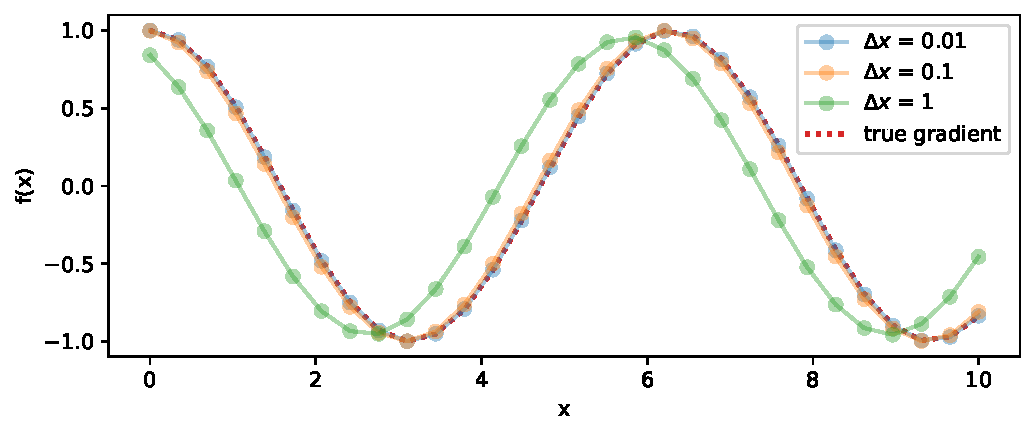
\includegraphics{./autodiff_files/figure-pdf/fig-finite-1-output-1.pdf}

}

\caption{\label{fig-finite-1}Finite difference gradient calculations for
the function \texttt{y=sin(x)}, varying the distance between the
evaluated points.}

\end{figure}

\begin{figure}

{\centering 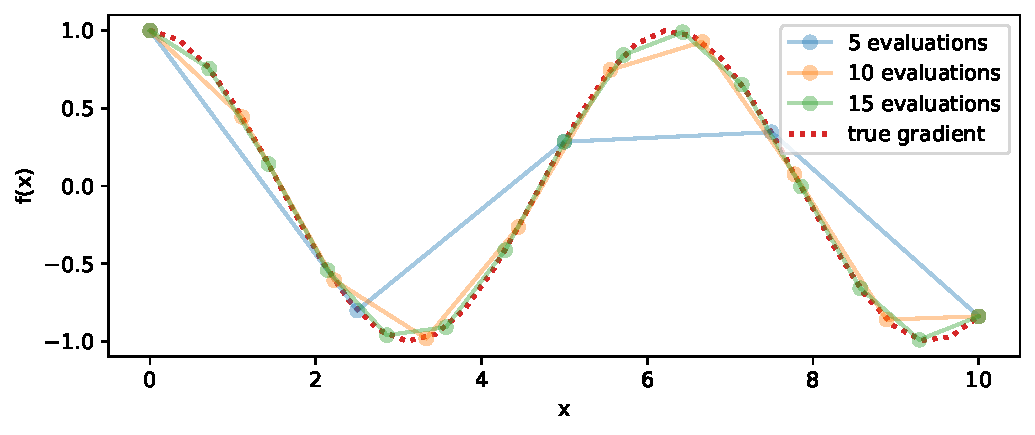
\includegraphics{./autodiff_files/figure-pdf/fig-finite-2-output-1.pdf}

}

\caption{\label{fig-finite-2}As in Figure~\ref{fig-finite-1}, but
varying the number of gradient evaluations with a fixed step size of
1e-4.}

\end{figure}

\hypertarget{symbolic-differentiation}{%
\subsection{Symbolic differentiation}\label{symbolic-differentiation}}

Symbolic differentiation endeavors to calculate gradients through
algebraic symbols, just like doing it on pen and paper. This approach
will definitely appeal at first sight to those that have done any kind
of calculus -- if we want to differentiate a function that implements
\(y = x^2\), then we will instantly think of \(2x\), not of
Jacobian-vector products or the like. In this sense, the gradients of
the functions produced are analytical. However, even for a simple
program, these expressions can swell easily to become horrifically
complex compared to the resulting programs from autodiff.

We'll omit any further discussion for now for the sake of brevity, but
for a much more thorough comparison between this and other methods
compared to automatic differentiation, I'll direct your attention to the
nicely-written notebook here that I looked at for inspiration while
writing this whole section: (Heinrich 2020).

\hypertarget{machine-learning}{%
\chapter{Machine learning}\label{machine-learning}}

The blanket term \textbf{machine learning} indicates a shift in mindset
for how computers complete a given task. When presented with such a
task, one may try to solve it through a pen and paper worked conceptual
solution. It is then up to us to tell the computer -- in excruciating
detail in it's own language -- each of the individual steps needed to
implement the solution we came up with. This is known as
\emph{programming} a computer. But what if there was a way to show the
computer many examples of our problem, and use an algorithm to
\emph{learn} a good solution by updating some internal state?

That's machine learning! We find some inspiration for this in a quote
from the fantastically written essay in (Samuel 1962), which is stated
in the context of comparing human-written programs to possibly learned
ones:

\begin{quote}
There are many mental processes that people are called upon to perform
that cannot be, or at least have not been, reduced to a simple set of
rules. Take the process of playing a game of chess, not of simply
adhering to the rules of the game, but rather the process of playing a
good game against an intelligent opponent. There are no known procedures
for guaranteeing a win, and yet people learn to play the game and some
few become very proficient. 
\end{quote}
\hfill-- \textit{Arthur L. Samuel}

The basic idea (also made reference to in that essay) is this: maintain
some internal state -- literally just a set of numbers, which could
e.g.~pick a pre-defined strategy based on a value -- and then update
that internal state in some way by checking the performance. This rather
simple statement carries a lot of ambiguous ideas, such as

\begin{itemize}
\tightlist
\item
  a notion of internal state
\item
  some way to combine that state with data to produce a result
\item
  a performance metric to assess the result after applying the state
\item
  an update rule to improve the value of the state based on the
  performance
\end{itemize}

These ideas form the cornerstone of machine learning approaches, and
we'll unpack them all in detail below. Before continuing though, it's
worth noting the distinction between \emph{machine} learning and
\emph{deep} learning -- the latter is a subset of the former, and refers
to a particular paradigm involving complex neural networks. Machine
learning makes no assumptions on the form of the machine itself.

Machine learning methods follow a shared set of abstract steps: given a
dataset, we

\begin{itemize}
\tightlist
\item
  define a \textbf{model} with \textbf{parameters} \(\varphi\) (where
  the model is a way to combine \(\varphi\) with the data)
\item
  construct a measure of performance for the model, called the
  \textbf{objective function}
\item
  \textbf{fit} the model to the dataset through some update rule
\item
  use the \emph{learned} model to perform \textbf{inference} (apply the
  model to new data)
\end{itemize}

We can see this workflow reflected in the API of modern software
packages, such as \texttt{scikit-learn} (Buitinck et al. 2013) and
\texttt{keras} (Chollet et al. 2015). Using this framework and
terminology, we'll explore some useful models, reflecting on the
developments that have occurred as a by-product of the modern era of
computing.

\hypertarget{neural-networks-and-deep-learning}{%
\section{Neural networks and deep
learning}\label{neural-networks-and-deep-learning}}

A model that would certainly be useful is one that can model the
solution to any task at all. \textbf{Neural networks} are indeed this
class of model; inspired by the way the brain handles the processing of
information, they are proven to be \emph{universal approximators},
i.e.~given a \emph{continuous function} \(g(\mathbf{x})\), where
\(\mathbf{x}\) is an arbitrary-length vector of real-valued inputs,
there exists a value of parameters \(\varphi\) such that a neural
network \(f(\mathbf{x}, \varphi)\) satisfies

\begin{equation}\protect\hypertarget{eq-approx}{}{
|g(\mathbf{x}) - f(\mathbf{x}, \varphi)| < \epsilon~~~\forall~\mathbf{x},~\text{for }\epsilon>0~.
}\label{eq-approx}\end{equation}

This is great! Though, it's not necessarily this property that makes
neural networks so popular, it's more the fact that we can practically
attain this performance. Said another way, it's not just that there
exists \(\varphi\), but that we can often find it in real life! This can
be attributed both to the effectiveness of \emph{gradient descent} as a
learning algorithm, and the software/hardware that we have access to
that breathes life into the training process.

So: what \emph{is} a neural network in the first place?

At its simplest, a neural network is a sequence of location-scale
transforms of the input data, with non-linear ``activation'' functions
applied in-between to allow for non-linear modelling capabilities. This
type of neural network is referred to as a \textbf{multi-layer
perceptron} (MLP) or a \textbf{feed-forward network} (both namings given
since I use them interchangeably in later sections). At its most complex,
there's a lot of funky ways to transform the data, including
self-attention, convolutions, graph structure, and all sorts of other
stuff. These types of specialized ``architectures'' are beyond the scope
of what we'll look at here, but are incredibly important for introducing
inductive bias that helps to more efficiently identify useful
information within the data.

\begin{figure}

{\centering 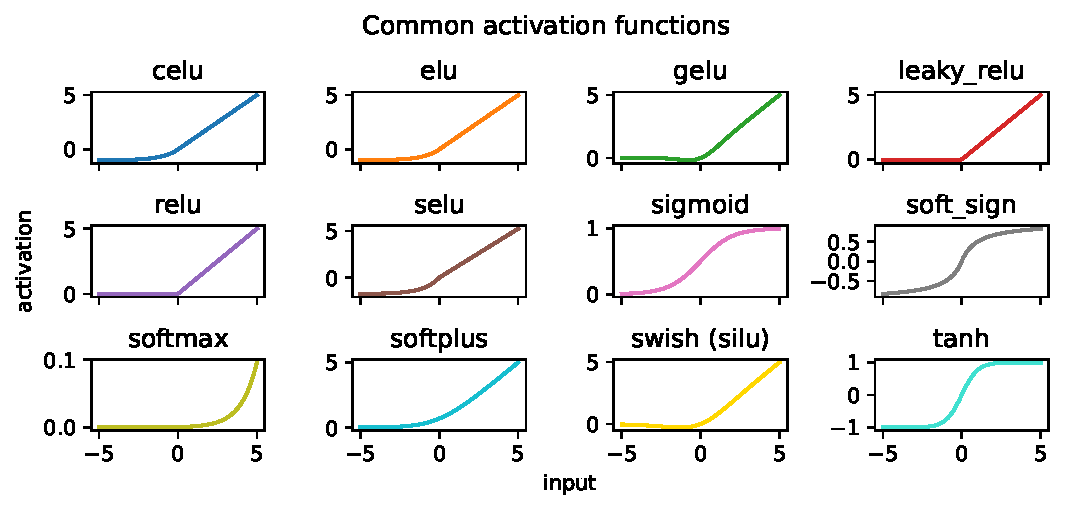
\includegraphics{./ml_files/figure-pdf/fig-activations-output-1.pdf}

}

\caption{\label{fig-activations}Commonly used activation functions,
taken from the Python library JAX.}

\end{figure}

The ingredients to a MLP are the \textbf{weights} \(w\), the
\textbf{biases} \(b\), and the \textbf{activation functions} \(\sigma\).
The weights represent the scale transform, and the bias the location
transform. On the other hand, the activation function plays the role of
``bending'' the output such that we can model non-linear effects,
i.e.~anything with realistic complexity. Examples of common activation
functions can be found in Figure~\ref{fig-activations}, where there are
all sorts of flavors to choose from, each with their own quirks (ReLU
and its variants have been the gold standard for some time).

You'll typically see all this represented in a ball-and-stick diagram,
e.g. Figure~\ref{fig-ballandstick}. Each series of balls represents one
set of computations with the weights, biases, and activation functions
that are within that layer. The outputs from this are called activations
(just to reference the application of the activation function). The
thing we call a \textbf{layer} is then each set of parallel computations
of this nature, which are then aggregated into the set of inputs to the
next layer (if it exists, else it's just the network output). Don't get
too hung up on this definition of the word ``layer'' though, it sort of
breaks down when looking at modern architectures with very detailed
computation steps.

\begin{figure}

{\centering 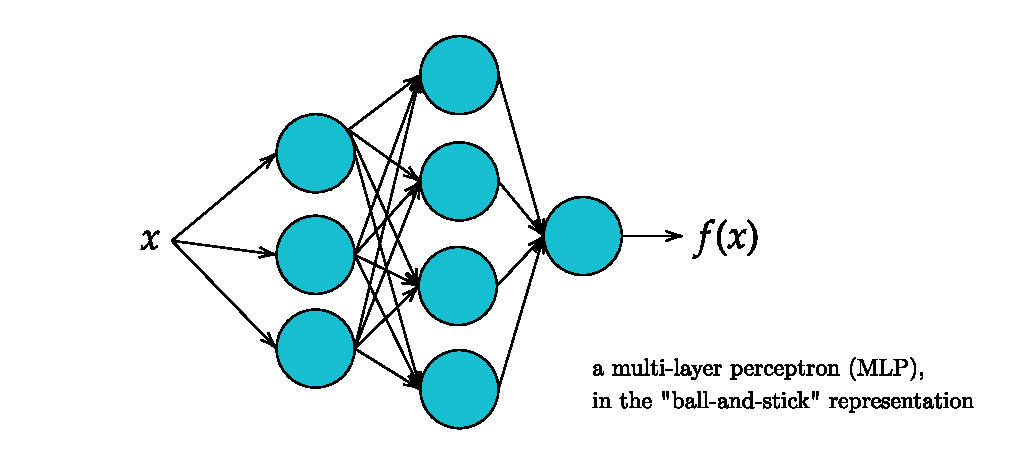
\includegraphics{./images/mlp.pdf}

}

\caption{\label{fig-ballandstick}The ``ball-and-stick'' representation
of a MLP.}

\end{figure}

\hypertarget{whats-a-layer-in-a-mlp}{%
\subsection{What's a ``layer'' in a MLP?}\label{whats-a-layer-in-a-mlp}}

Here's a compact formula for a computation of a single layer. Given a
set of \(n\) activations from the previous layer (0th layer meaning just
the data points), and \(k\) neurons in layer \(i\), the output of
applying the neurons to the activations to obtain the \(i+1\)th layer is
represented as a matrix equation:

\[
\textcolor[HTML]{17BECF}{
\underbrace{\left[\begin{array}{c}
a_0^{(i)} \\
a_1^{(i)} \\
\vdots \\
a_n^{(i)}
\end{array}\right]}_{\text{activations for layer }i+1}}=\sigma\left(\textcolor[HTML]{FF7F0E}{\underbrace{\left[\begin{array}{cccc}
w_{0,0} & w_{0,1} & \cdots & w_{0, n} \\
w_{1,0} & w_{1,1} & \cdots & w_{1, n} \\
\vdots & \vdots & \ddots & \vdots \\
w_{k, 0} & w_{k, 1} & \cdots & w_{k, n}
\end{array}\right]}_{\text{weight matrix}}}\textcolor[HTML]{1F77B4}{\underbrace{\left[\begin{array}{c}
a_0^{(i)} \\
a_1^{(i)} \\
\vdots \\
a_n^{(i)}
\end{array}\right]}_{\text{activations for layer }i}}+\textcolor[HTML]{2CA02C}{\underbrace{\left[\begin{array}{c}
b_0 \\
b_1 \\
\vdots \\
b_n
\end{array}\right]}_{\text{bias vector}}}\right)
\]

\[
\Rightarrow \textcolor[HTML]{17BECF}{\mathbf{a}^{(i+1)}} = \sigma\left(\textcolor[HTML]{FF7F0E}{\mathbf{W}}\textcolor[HTML]{1F77B4}{\mathbf{a}^{(i)}} + \textcolor[HTML]{2CA02C}{\mathbf{b}}\right)~,
\]

where applying the activation \(\sigma\) is distributed to its elements,
i.e. \begin{equation}\protect\hypertarget{eq-layer}{}{
\sigma\left(\left[\begin{array}{l}
x \\
y \\
z
\end{array}\right]\right)=\left[\begin{array}{l}
\sigma(x) \\
\sigma(y) \\
\sigma(z)
\end{array}\right]~.
}\label{eq-layer}\end{equation}

This is essentially the definition of a neuron (the ball in the
ball-and-stick diagram shown in Figure~\ref{fig-ballandstick}): a neuron
is the \(j\)th function in a layer \(i\) that maps the activations
\(\mathbf{a}^{(i)}\) from the previous layer into the \(j\)th element of
the \(i+1\)th activation vector \(\mathbf{a}^{(i+1)}\), with a
functional form as indicated in Equation~\ref{eq-layer}. The sticks in
that diagram would represent the elements of the weight matrix
\(\mathbf{W}\), with missing connections between neurons \(a\) and \(b\)
corresponding to zeroing out the \(w_{a,b}\) term in the weight matrix.

If we put the weights and biases for each layer all into one vector of
parameters, that's what we've been calling \(\varphi\), which represents
the entire internal state of a neural network. If we then bottle up the
way we apply \(\varphi\) to the data within the function \(f\) --
whether that be as simple as the MLP above or something more complex --
we can compactly represent a neural network as
\(f(\mathbf{x}, \varphi)\) as above in Equation~\ref{eq-approx}.

Since a neural network is a sequence of applications of
Equation~\ref{eq-layer}, it's differentiable with respect to the
parameters \(\varphi\) (and even if it's more complex, this
differentiability is always made to be present). That means we can
optimize our neural network with \textbf{gradient descent}, which we
spent considerable time on in the previous section.

One extra thing to mention is the different type of architectures that
go beyond this simple MLP framing. We can think about these
architectures as a kind of inductive bias on the space of possible
functions that could be learned, e.g.~through some kind of specific
manipulations that take advantage of the format of the input data
(sequences, images, sets etc.). To highlight a few:

\begin{itemize}
\item
  \textbf{Convolutional neural networks} (Krizhevsky, Sutskever, and
  Hinton 2012) are one of the first types of domain-specific
  architecture, and manipulate an image through convolutional filters
  that measure local image features through things like pooling.
\item
  \textbf{Transformers} (Vaswani et al. 2017) perform fantastically well
  for sequential data (e.g.~natural language), but have even shown
  generalization to other domains like images (Dosovitskiy et al. 2020).
  They use a mechanism called \emph{self-attention} to extract
  information from sequential inputs, and are probably the most
  important architecture that exists at the time of writing in terms of
  their ability to generalize and scale.
\item
  \textbf{Deep sets} (Zaheer et al. 2017) is a method that incorporates
  the bias of the input data being an unordered collection. They have
  found use in e.g.~particle physics (Komiske, Metodiev, and Thaler
  2019), where objects like jets and their properties exist in unequal
  amounts across events, but without any specific ordering (though we've
  typically ordered them by \(p_T\) and then treated them as a sequence
  in the past).
\item
  \textbf{Geometric deep learning} (Bronstein et al. 2021) generalizes a
  lot of the above, and casts things in the language of equivariances
  and graphs, spawning the idea of e.g.~graph neural networks (Scarselli
  et al. 2009).
\end{itemize}

There are countless other architectures, but we will focus on a
particular neural network method (not necessarily an architecture) in
the next section, as it makes up one of my applications, so we'll spend
a bit of extra time to sufficiently ground that work.

\hypertarget{sec-flows}{%
\section{Normalizing flows}\label{sec-flows}}

A \textbf{normalizing flow} is a trainable density estimator based on
neural networks that admits both sampling and a tractable likelihood.
Flows model a vector \(\mathbf{x} \in \mathbb{R}^D\) from an underlying
distribution \(p_X(\mathbf{x})\) as a transformation
\(\mathbf{x} = T(\mathbf{u})\), where \(\mathbf{u} \in \mathbb{R}^D\) is
a vector of samples drawn from a chosen distribution
\(p_U(\mathbf{u})\). We refer to the data distribution
\(p_X(\mathbf{x})\) as the \textbf{target distribution} that we're
trying to model, and to \(p_U(\mathbf{u})\) as the \textbf{base
distribution} that we transform to do this. This base distribution is
normally something simple like a normal distribution, which offers some
guarantees as to making the flow a universal density approximator
(details in Papamakarios et al. (2019)).

How does this work? The transform \(T\) is the key, and is the thing
we'll be training in practice. We start by pointing out the defining
property of flows, which is the requirement that \(T\) is both

\begin{itemize}
\tightlist
\item
  \emph{differentiable} (the Jacobian of the transformation
  \(J_T(\mathbf{u}) \in \mathbb{R}^{D\times D}\) exists, where
  \(J_T(\mathbf{u})\) is defined as in Equation~\ref{eq-jacobian})
\item
  \emph{invertible} (the inverse transformation \(T^{-1}(\mathbf{x})\)
  exists).

  \begin{itemize}
  \tightlist
  \item
    \(T^{-1}(\mathbf{x})\) is also required to be differentiable for
    flows!
  \end{itemize}
\end{itemize}

Given these properties, we can invoke the change of variables formula
from \(X\) to \(U\), which relates the target and base distributions by
the determinant of the Jacobian matrix:

\[
p_X(\mathbf{x}) = p_U(\mathbf{u}) \left|\det{J_T(u)} \right|^{-1}.
\]

Here, \(\mathbf{u}\) is calculated as the inverse transformation
\(\mathbf{u} = T^{-1}(\mathbf{x})\) since we want the exact
\(\mathbf{u}\) for our particular \(\mathbf{x}\) when evaluating the
likelihood. We've also exploited the fact that the determinant of the
inverse of a matrix is the inverse of the determinant.

You may have noted our extra requirement that the inverse transform is
also differentiable --- the existence of the Jacobian
\(J_{T^{-1}}(\mathbf{x})\) lets us write the change of variables above
in terms of only \(T^{-1}\) and \(\mathbf{x}\):

\begin{equation}\protect\hypertarget{eq-flowlhood}{}{
p_X(\mathbf{x}) = p_U(T^{-1}(\mathbf{x})) \left|\det{J_{T{-1}}(\mathbf{x})} \right|.
}\label{eq-flowlhood}\end{equation}

These equations form the basis for constructing a flow, where we
implement the transform \(T\) by using a neural network to control its
parameters (e.g.~a location-scale transform, where the location and
scale are provided by a network).

One advantage of having a differentiable and invertible \(T\) is that we
can compose multiple transforms in a row, with the result itself being
both differentiable and invertible. Specifically, we can write, for
\(T=T_1 \circ T_2\):

\[
T^{-1} = (T_1 \circ T_2)^{-1} = T_2^{-1} \circ T_1^{-1}~,
\] \[
\det{J_T(\mathbf{u})} = \det{J_{T_1 \circ T_2}(\mathbf{u})} = \det{J_{T_2}(T_1(\mathbf{u}))}\det{J_{T_1}(\mathbf{u})}~.
\]

Knowing that we can stack transformations freely, we have a similar
paradigm to neural networks, where stacking more ``layers'' (here,
transforms) could bring about a more expressive model. This is the
``flow'' part of a normalizing flow: a series of samples from \(p_U\)
are flowing through a series of transforms \(T\) to arrive at something
like the target density \(p_X\). The ``normalizing'' part comes from
going the other direction via \(T^{-1}\), where data samples are
``normalized'' back to the base distribution\footnote{The naming is a
  bit extra, I know. But at least it's not another play on ``attention
  is all you need''.}.

There are many types of transforms one can choose to satisfy these
requirements (which can be partitioned into a bijective ``transformer''
and a non-bijective ``conditioner''), but I'll omit everything but the
one I used in Section~\ref{sec-maf}, and direct you to (Papamakarios et
al. 2019) for a much more comprehensive review.

\hypertarget{sec-trainflow}{%
\subsection{Training a flow}\label{sec-trainflow}}

The goal is clear: we want to make our base distribution look like the
target distribution. How do we quantify this?

Recall from Section~\ref{sec-KL} that we have access to the
KL divergence between two probability distributions through the expected
difference in log-likelihood under the true distribution (or approximate
distribution, noting the asymmetric result depending on our choice).
Denoting the predicted distribution from the flow as
\(q_X(\mathbf{x}; \theta)\) (where \(\theta\) comprises both the
parameters of the base density \(\gamma\) and the parameters of the
transform \(\phi\)), and the target density as \(p_X(\mathbf{x})\), we
can write this explicitly as

\[
D_{\mathrm{KL}}[p_X(\mathbf{x}) || q_X(\mathbf{x}; \theta)] = -\mathbb{E}_{p_X(\mathbf{x})}\left[\log q_X(\mathbf{x}; \theta)\right] + \mathrm{constant}
\] \[
\Rightarrow = -\mathbb{E}_{p_X}\left[\log p_U(T^{-1}(\mathbf{x} ;\phi); \gamma) + \log |\det J_{T^{-1}}(\mathbf{x}; \phi)|\right] + \mathrm{constant}~,
\]

where we've substituted our expression for the flow likelihood in
Equation~\ref{eq-flowlhood}.

This is a quantity we'd like to minimize, as to make \(p_X\) and \(q_X\)
as ``close'' as possible. In practice, we're likely going to have to
substitute the expectation over the true (unknown) distribution with a
Monte Carlo estimate using our data samples \({x_i}_{i=1}^{N}\), which
turns this equation into

\[D_{\mathrm{KL}}[p_X(\mathbf{x}) || q_X(\mathbf{x}; \theta)] \approx-\frac{1}{N} \sum_{i=1}^N \log p_{\mathrm{u}}\left(T^{-1}\left(\mathbf{x}_i ; {\phi}\right) ; \gamma\right)+\log \left|\operatorname{det} J_{T^{-1}}\left(\mathbf{x}_i ; {\phi}\right)\right|~,\]

plus a constant term that's omitted for legibility. This comes out to effectively minimizing the negative log-likelihood of
the flow model on the data samples -- we're just fitting the model with
maximum likelihood, as defined in Section~\ref{sec-mle}! This is one
example of how we can train a flow -- we minimize this objective with
respect to parameters \(\theta\), by e.g.~gradient descent, since this
is a differentiable expression in \(\theta\).

\hypertarget{sec-maf}{%
\subsection{Masked Autoregressive Flows}\label{sec-maf}}

A specific type of flow that we'll encounter in the wild later is the
\textbf{masked autoregressive flow} (Papamakarios, Pavlakou, and Murray
2017). The approach that this flow takes to density modelling is as
follows:

When modelling a distribution across multiple random variables, one can
break down their joint density into a product of conditional
distributions through the probability chain rule as in
Equation~\ref{eq-prob-chain-rule}, and models these conditional
distributions explicitly:

\[
p(x_1, \dots, x_N) = p(x_1)p(x_2 | x_1)p(x_3|x_2, x_1)\dots p(x_N | x_{N-1}, \dots, x_1)
\] \[
=\prod_{i=1}^Np(x_i|\mathbf{x}_{j<i})
\]

Here, we've arbitrarily labelled our random variables \(x_i\) with
indicies \(i\) from \(1\) to \(N\), and use these to construct our
conditional distributions. Note, however, that we could shuffle the
order of our random variables, then reassign them the index of their
place in the array, and the relation would still hold. Despite this, the
only important thing is that each conditional distribution assigned to
\(x_i\) depends \emph{only} on those \(x_j\) for which \(j<i\),
\emph{regardless of the initial variable ordering}. This is known as the
\textbf{autoregressive property}.

One can model this relationship using a neural network in a \emph{single
forward pass.} By constructing a feed-forward network with equal input
and output dimensionality, and assigning the same ordering to the input
and output, we can simply drop (or \textbf{mask}) those connections for
each output \(i\) with all input variables that have index \(j<i\). This
way, there is no possible computational path between each output and the
variables that come before that output in the ordering, meaning that the
value of that output will be able to capture the nature of the relevant
conditional \(p(x_i | \mathbf{x}_{j<i})\). These aspects together form a
\textbf{masked, autoregressive} network.

This idea was first used in (Germain et al. 2015), which used it to
output the density directly in one forward pass by having the outputs
correspond to the individual conditional distributions. However, to use
this network in a flow, which transforms one distribution to another, we
can instead use the outputs of the neural network to parametrize the
transform \(T\). The result is known as a \textbf{masked autoregressive
flow} (MAF), and was introduced in (Papamakarios, Pavlakou, and Murray
2017).

The MAF as I used it involved a fairly simple implementation of \(T\) --
a location scale transform:

\[
T(\mathbf{u}; \alpha, \beta) = \alpha \cdot \mathbf{u} + \beta~,
\]

where \(\alpha, \beta\) are the scale and location
parameter vectors respectively. These are \emph{vectors} because there's
one entry corresponding to each entry in \(\mathbf{u}\), where the
individual parameters \(\alpha_i, \beta_i\) are coming from the \(i\)th
output of a neural network (or more precisely, the \(i\)th pair of
outputs, since we have two values \(\alpha_i, \beta_i\) for every one
input \(u_i\)), which has parameters itself \(\phi\). Training the flow
is then done as in Section~\ref{sec-trainflow}, with the masking
mechanism from earlier in this section being put in place.

As a bonus, there's a simple way to condition this transform on side
information \(\mathbf{y}\) that provides context: we can just add
\(\mathbf{y}\) as an extra input to the network (or multiple inputs if
there's more than one variable), and have it mix with every input, since
each conditional distribution would also include \(\mathbf{y}\). We then
have a MAF that can perform \textbf{conditional density estimation},
i.e.~estimate \(p(x_1, \dots, x_N| \mathbf{y})\).

\part{Applications}

\hypertarget{data-analysis-in-high-energy-physics-as-a-differentiable-program}{%
\chapter{Data Analysis in High-Energy Physics as a Differentiable
Program}\label{data-analysis-in-high-energy-physics-as-a-differentiable-program}}

This is the title track of this thesis, and rightly so; it dominated
metrics in both my time spent and headspace given for any of the topics
I've written about. I feel incredibly privileged to have worked on
something like this, which is fairly self-contained, and draws upon
themes from both machine learning and statistical inference in order to
make headway in addressing a long-standing issue: \emph{systematic-aware
optimization}. What's even cooler is that it goes further than this,
opening up a whole variety of possibilities to optimize with the whole
statistical inference procedure in the loop, and rethink the ways in
which we can improve our workflows. I hope you enjoy it!

\hypertarget{motivation}{%
\section{Motivation}\label{motivation}}

Given the success of the Standard Model, analysis of data from the LHC
usually occurs for two reasons:

\begin{itemize}
\tightlist
\item
  Precisely measuring Standard Model processes to look for small
  deviations from their predicted values
\item
  Searching for new physics signatures as predicted by models beyond the
  Standard Model
\end{itemize}

When analyzing data in this way, we'll have lots of free parameters to
tune. These can be as simple as a threshold value that you limit the
\(p_T\) to, or as complicated as the weights and biases that determine a
neural network for identifying \(b\)-jets. We can of course choose any
values for these quantities to do our analysis, but the resulting
physics that follows may suffer as a result. As such, we're likely to
try some kind of optimization to improve the answers to our physics
questions. How do we do this in practice?

In either case above, there is a notion of {signal} (what you're looking
for) and {background} (everything else). Generally, we then try to
choose a parameter configuration that can separate (or discriminate) the
signal from the background, allowing us to extract just the data we
think is relevant to the physics process we're looking at. As an
example, machine learning models are often trained using the
\textbf{binary cross-entropy} loss as an objective, which corresponds to
optimizing the ability of the model to identify whether an event
originated from signal or background processes. A closely related goal
is the \textbf{Asimov significance} in the case of signal and background
event counts \(s\) and \(b\) with \emph{no uncertainty} on either
quantity. The formula for this stems from assuming a Poisson likelihood
function as in Section~\ref{sec-hifa}, and is equal to

\begin{equation}\protect\hypertarget{eq-asimov-significance}{}{
Z_A = \sqrt{2\sum_{i\in \mathrm{bins}}((s_i + b_i)(\log{(1 + s_i / b_i)}) - s_i)}~.
}\label{eq-asimov-significance}\end{equation}

As indicated in the sum, these counts can be spread across different
bins in the case where your data is a histogram, but the formula is more
commonly reduced to the 1-bin scenario that just deals with the overall
numbers of signal and background events. In this case, we can then
Taylor expand the logarithm to get

\[Z_A = \sqrt{2((s+b)(s/b + \mathcal{O}(s/b) - s)} \approx s/\sqrt{b}~~~\mathrm{for}~s<<b.\]

This makes it much clearer to see that optimizing with respect to
\(Z_A\) is just a fancier way of trying to increase the amount of signal
compared to the amount of background, which is directly analogous to
separating signal from background, just as binary cross-entropy would
do.

Now, this is all very sensible of course (we want to discover our
signal), but this approach has some shortcomings that distance the
efficacy of the resulting configuration from our physics goals. A recent
review of deep learning in LHC physics (Guest, Cranmer, and Whiteson
2018) lets us in on why:

\begin{quote}
(\ldots) tools are often optimized for performance on a particular task
that is \textbf{several steps removed from the ultimate physical goal}
of searching for a new particle or testing a new physical theory.
\end{quote}

\begin{quote}
(\ldots) sensitivity to high-level physics questions \textbf{must
account for systematic uncertainties}, which involve a nonlinear
trade-off between the typical machine learning performance metrics and
the systematic uncertainty estimates.
\end{quote}

This is the crux of the issue: we're not accounting for uncertainty. Our
data analysis process comes with many sources of systematic error, which
we endeavour to model in the likelihood function as nuisance parameters.
However, optimizing with respect to any of the above quantities isn't
going to be aware of that process. We need something better.

Okay, I hear you: blah blah this is all just talk\ldots{} let's prove
this scenario needs addressing with an example!

\hypertarget{sec-simple-anal}{%
\subsection{A simplified analysis example, both with and without
uncertainty}\label{sec-simple-anal}}

Let's define an analysis with a predicted number of signal and
background events (e.g.~from simulation), with some uncertainty on the
background estimate. We'll abstract the analysis configuration into a
single parameter \(\phi\) like so:

\[s = 15 + \phi \] \[b = 45 - 2 \phi \] \[\sigma_b = 0.5 + 0.1\phi^2 \]

Note that \(s \propto \phi\) and \(\propto -2\phi\), so increasing
\(\phi\) corresponds to increasing the signal/backround ratio. However,
our uncertainty scales like \(\phi^2\), so we're also going to
compromise in our certainty of the background count as we do that. This
kind of tradeoff between \(s/b\) ratio and uncertainty is important for
the discovery of a new signal, so it may be that can't get away with
optimizing \(s/b\) alone, as the \(p\)-value may be worse!

Let's start by visualizing the model itself, which we do for three
values of \(\phi\) as an example in Figure~\ref{fig-simple-model}.

\begin{figure}

{\centering 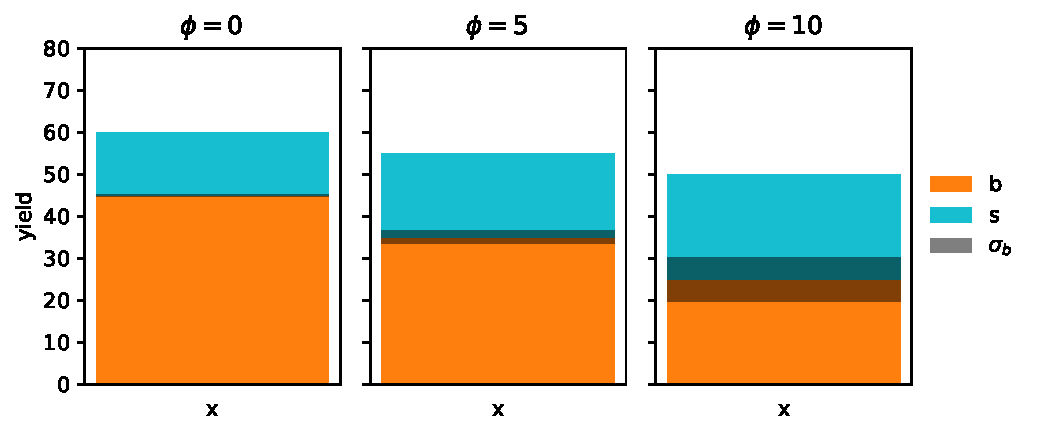
\includegraphics{./diffprog-hep_files/figure-pdf/fig-simple-model-output-1.pdf}

}

\caption{\label{fig-simple-model}Plot of the predicted counts from our
model at three values of \(\phi\).}

\end{figure}

Using this very simple histogram, we can form a statistical model as if
we're using Section~\ref{sec-hifa} principles, which would look
something like

\begin{equation}\protect\hypertarget{eq-simplemodel}{}{
p(x | \mu) = \mathrm{Poisson}(x | \mu x^{\mathrm{sig}}  + \gamma x^{\mathrm{bkg}})\,\mathrm{Normal}(y | \gamma, 1)~,
}\label{eq-simplemodel}\end{equation}

where \(\gamma\) is a continuous description of \(\sigma_b\) that we get
from interpolating between the yields, just like in the HistFactory
approach, which has the constraint term
\(\mathrm{Normal}(y | \gamma, 1)\) attached to penalize fitting a value
of \(\gamma\) that differs largely from the information provided by
\(\sigma_b\).

Using this likelihood, we can calculate the expected discovery
\(p\)-value by doing a hypothesis test using the observed data as the
Asimov dataset for the nominal model \(\mu, \gamma = 1\). We can plot
this across all the values of \(\phi\), and see what value gives us the
lowest \(p\)-value (in practice, scanning over the space is
computationally impossible for a given analysis configuration and a
complicated model). We do this in Figure~\ref{fig-simple-model-pval},
where we include the result using a model both with and without
uncertainty. Notice how much the curves differ; if we optimized the
model without uncertainty (i.e.~optimize for signal/background
separation only), we'd end up at the \emph{worst} solution! This is
pathologically constructed of course, but it goes to show that these
objectives don't talk to each other directly.

\begin{figure}

{\centering 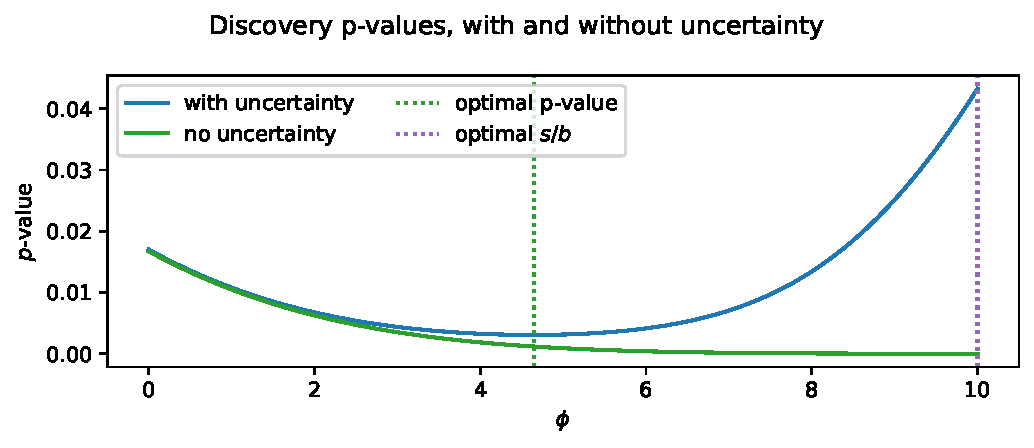
\includegraphics{./diffprog-hep_files/figure-pdf/fig-simple-model-pval-output-1.pdf}

}

\caption{\label{fig-simple-model-pval}Plot of the calculated \(p\)-value
from using our statistical model across of \(\phi\), both including the
uncertainty and neglecting it.}

\end{figure}

If we optimize this analysis then, we want to arrive at the value of
\(\phi\) at the dotted green line (around \textasciitilde4.3 or so),
which gives us the benefit of rejecting the background hypothesis more
strongly when the signal exists in the data. This is made possible if we
use the \(p\)-value as our objective -- it clearly accounts for the
uncertainty!

The reason for this makes sense: in these physics likelihoods, we're
careful to include all the details of the systematic uncertainties that
we're able to quantify by constructing nuisance parameters that vary the
shape and normalization of the model. From here, to calculate the
\(p\)-value, we then construct the \textbf{profile likelihood ratio} as
a test statistic, which accounts for these systematic uncertainties by
fitting the value of the nuisance parameters depending on the hypothesis
you test (see Section~\ref{sec-hyptests} for more).

All this makes the \(p\)-value seem like a good candidate for an
objective function! So why haven't we used this already?

As emphasized in Chapter~\ref{sec-gradient-descent}, if we want to
perform optimization using gradient-based methods,\footnote{We don't
  have to use gradient based methods! They're just very well implemented
  and studied, as well as enabling things like this paradigm.} then we
need the objective that we optimize to be \emph{differentiable}. This is
not immediately the case for the \(p\)-value -- we would have to be able
to differentiate through all stages of the full calculation, including
model building, profiling, and even histograms, which are not generally
known for their smoothness. But say we were able to decompose this
complicated pipeline into bite-size chunks, each of which we can find a
way to take gradients of. What becomes possible then? This begins our
view of \textbf{data analysis in high-energy physics as a differentiable
program}.

In the following sections, we'll take a collider physics analysis apart
step-by-step, then see how we can employ tricks and substitutes to
recover gradients for each piece. After that, we'll explore the ways
that we can use the result to perform gradient-based optimization of
different parts of the analysis with respect to physics goals. We'll
then do it all at once by \emph{optimizing a toy physics analysis from
end-to-end}, exploring the common example of a summary statistic based
on a neural network, accounting for uncertainties all the while.

\hypertarget{making-hep-analysis-differentiable}{%
\section{Making HEP Analysis
Differentiable}\label{making-hep-analysis-differentiable}}

The goal of this section is to study components within a HEP analysis
chain that are not typically differentiable, and show that when we
overcome this, we can employ the use of gradient-based optimization
methods -- both to optimize free parameters jointly, and to use
objectives we care about. From there, we'll examine the typical steps
needed to calculate the sensitivity of a physics analysis, and see how
we can make that whole chain differentiable at once, opening up a way to
incorporate the full inference procedure when finding the best analysis
configuration.

First, we're going to jump right in with an example to illustrate how we
can take advantage of gradient descent to optimize a typical problem
faced in collider physics analyses: choosing the best selection
criteria.

\hypertarget{a-simple-example-cut-optimization-with-gradient-descent}{%
\subsection{A simple example: cut optimization with gradient
descent}\label{a-simple-example-cut-optimization-with-gradient-descent}}

We begin with a toy signal and background distribution over some
variable \(x\), where the signal lies as a peak on top of an
exponentially decaying background, as shown in Figure~\ref{fig-exp-bkg}.

\begin{figure}

{\centering 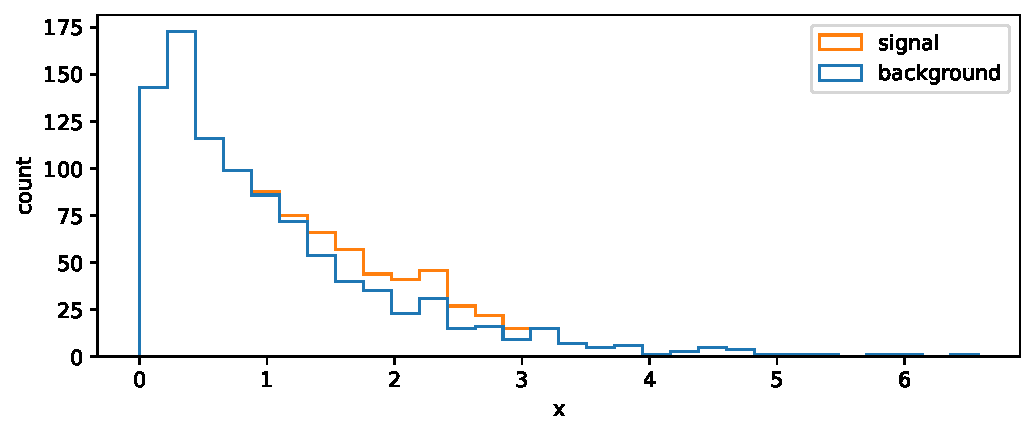
\includegraphics{./diffprog-hep_files/figure-pdf/fig-exp-bkg-output-1.pdf}

}

\caption{\label{fig-exp-bkg}Histogram of a situation with a simple
exponentially falling background and a small signal peak.}

\end{figure}

A quintessential operation for data filtering in HEP is the simple
threshold, also called a \textbf{cut}: we keep all data above (or below)
a certain value of the quantity we're concerned with. To increase the
significance (e.g.~as defined by Equation~\ref{eq-asimov-significance}),
we can try to remove data such that we increase the overall ratio of
signal to background. In Figure~\ref{fig-exp-bkg}, it looks like there's
not much signal for low values of \(x\), which motivates us to put a cut
at say \(x=1\). We can see the result of applying this cut in
Figure~\ref{fig-compare-cut}, where we've increased the Asimov
significance compared to using no cut at all.

\begin{figure}

{\centering 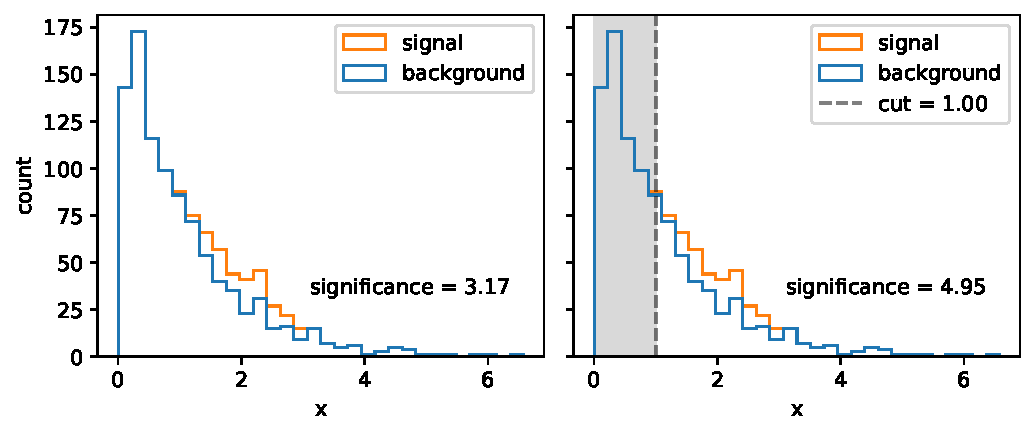
\includegraphics{./diffprog-hep_files/figure-pdf/fig-compare-cut-output-1.pdf}

}

\caption{\label{fig-compare-cut}Comparing the significance resulting
from applying a cut to no cut at all.}

\end{figure}

We had a nice go at a guess, but how do we pick the \emph{best} cut? For
this simple problem, it suffices to scan over the different
significances we'll get by cutting at each value of \(x\), then just use
the value with the highest significance. Doing this leads to the optimal
cut being around \(x=1.54\). In reality, though, this could be an
expensive procedure to do for a wide range of \(x\) and for many
different cut variables. This prompts the search for some kind of
intelligent optimization that can handle large dimensional parameter
spaces. Gradient descent is just that! But, to make it work, we need to
be able to calculate the gradient of the significance with respect to
the cut value -- something only possible if the cut itself is
differentiable (it isn't).

To see this, note that cuts are step functions, i.e.~logical less than
or more than statements. These can be viewed as applying weights to the
data -- 0 on one side of the threshold, and 1 on the other. If we change
the cut value, the events either keep their weight (0 change in
significance) or sharply gain/lose their weight value (discrete jump in
significance). We would then like to replace this thresholding with a
\emph{smooth} weight assignment such that the cut value varies smoothly
with the weights applied. What kind of operation can do this? We have
such a candidate in the \emph{sigmoid function} \(1/(1+e^{-x})\).

Normally, the sigmoid serves as a method to map values on the real line
to {[}0,1{]}, so we leverage this to be used as a cut by applying it to
data, which results in a set of weights for each point in {[}0,1{]}. (A
normal cut does this too, but the weights are all 0 or 1, and you drop
the 0s. One could similarly threshold on a minimum weight value here.)

Practically, we introduce slope and intercept terms that control the
sigmoid's \(x\) position and how ``hard'' the cut is:
\(1/(1+e^{-\mathrm{slope}(x-\mathrm{cut~value}})\). This slope allows us
to control the degree to which we approximate the cut as a thresholding
operation, with higher values of the slope meaning less approximation
(but this will also increase the variance of the gradients, as we're
getting closer to the discrete situation outlined previously). See the
sigmoid plotted with different slopes in Figure~\ref{fig-sigmoid}.

\begin{figure}

{\centering 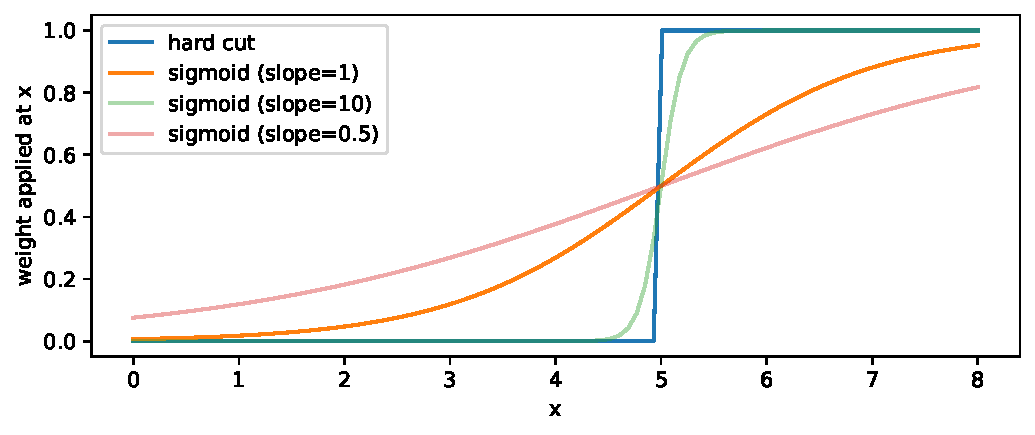
\includegraphics{./diffprog-hep_files/figure-pdf/fig-sigmoid-output-1.pdf}

}

\caption{\label{fig-sigmoid}Comparing the sigmoid to a regular hard cut
for different values of the sigmoid slope.}

\end{figure}

Now that we have a differentiable cut, we can see what the significance
scan looks like for both the differentiable and standard cases, shown in
Figure~\ref{fig-cut-scan-2}. It's an interesting plot; there's a clear
smoothing out of the overall envelope of the significance in comparison
to using the hard cut. However, the important thing is the
\textbf{coincidence of the maxima}: when optimizing, we'll use the
differentiable cut, but we'll plug the value of the cut position from
the optimization back in to the hard cut for our actual physics results.
This is a very important distinction - \emph{we don't use approximate
operations in the final calculation!} Moreover, since we can control the
degree to which we're approximating the significance landscape, one
could even imagine a fine-tuning of the slope when we're close to a
local minima during optimization, allowing us to make jumps more in-line
with the true optimum value (though this is not explored here).

\begin{figure}

{\centering 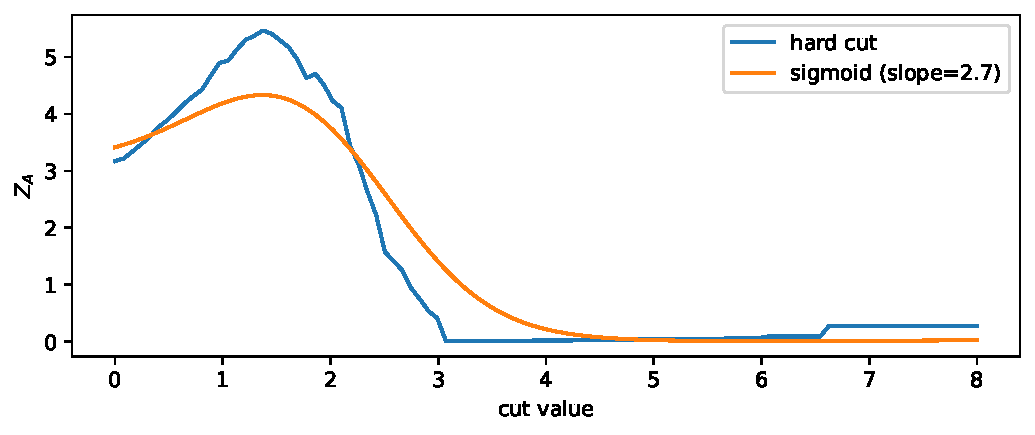
\includegraphics{./diffprog-hep_files/figure-pdf/fig-cut-scan-2-output-1.pdf}

}

\caption{\label{fig-cut-scan-2}A scan over all cut values to find the
best resulting Asimov significance -- both for the regular cut, and for
the sigmoid.}

\end{figure}

Now that we've done the groundwork, we can do the optimization and see
if we converge to the correct result! Using gradient descent and the
Adam optimizer with a learning rate of 1e-3, we find the cut shown in
Figure~\ref{fig-optimized-cut} (we optimize \(1/Z_A\) since we're doing
minimization). The significance (calculated with the \emph{hard} cut) is
extremely close to the best possible value, so I'd call this a success!

\begin{figure}

{\centering 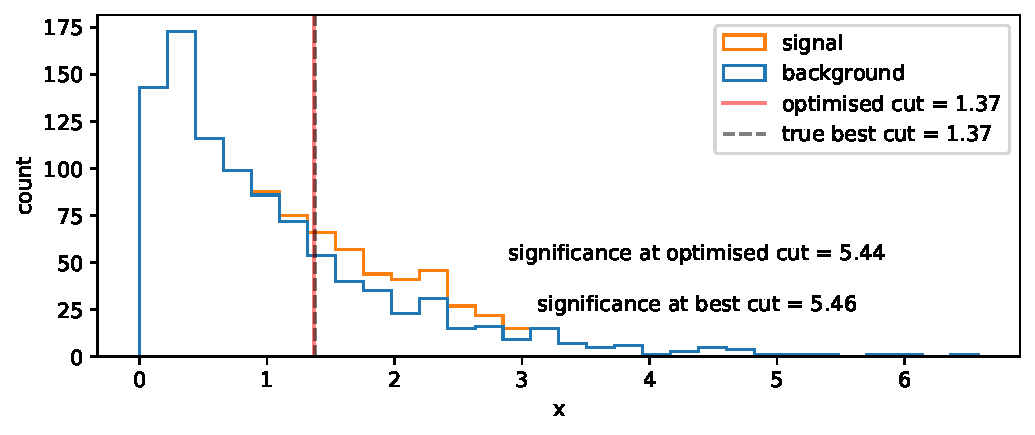
\includegraphics{./diffprog-hep_files/figure-pdf/fig-optimized-cut-output-1.pdf}

}

\caption{\label{fig-optimized-cut}The resulting cut from optimization
compared to the true best cut. Significances in both cases are shown.}

\end{figure}

\hypertarget{examining-a-typical-analysis}{%
\subsection{Examining a typical
analysis}\label{examining-a-typical-analysis}}

Now that we've looked at an example of the kind of thing we may want to
do, we can zoom out and look at the big picture. Given a pre-filtered
dataset, a commonly used analysis pipeline in HEP involves the following
stages:

\begin{enumerate}
\def\labelenumi{\arabic{enumi}.}
\item
  Construction of a learnable 1-D summary statistic from data (with
  parameters \(\varphi\))
\item
  Binning of the summary statistic, e.g.~through a histogram
\item
  Statistical model building, using the summary statistic as a template
\item
  Calculation of a test statistic, used to perform a frequentist
  hypothesis test of signal versus background
\item
  A \(p\)-value (or \(\mathrm{CL_s}\) value) resulting from that
  hypothesis test, used to characterize the sensitivity of the analysis
\end{enumerate}

We can express this workflow as a direct function of the input dataset
\(\mathcal{D}\) and observable parameters \(\varphi\):

\begin{equation}\protect\hypertarget{eq-neos}{}{
    \mathrm{CL}_s = f(\mathcal{D},\varphi) = (f_{\mathrm{sensitivity}} \circ f_{\mathrm{test\,stat}} \circ f_{\mathrm{likelihood}}  \circ f_{\mathrm{histogram}}  \circ f_{\mathrm{observable}})(\mathcal{D},\varphi).
}\label{eq-neos}\end{equation}

Is this going to be differentiable? To calculate
\(\partial \text{CL}_s / \partial \varphi\), we'll have to split this up
by the chain rule into the different components, which can be written
verbosely as

\begin{equation}\protect\hypertarget{eq-analysis-chain-rule}{}{
\frac{\partial\,\mathrm{CL}_s}{\partial \varphi} = \frac{\partial f_{\mathrm{sensitivity}}}{\partial f_{\mathrm{test\,stat}}}\frac{\partial f_{\mathrm{test\,stat}}}{\partial f_{ \mathrm{likelihood}}} \frac{\partial f_{\mathrm{likelihood}}}{\partial f_{\mathrm{histogram}}}   \frac{\partial f_{\mathrm{histogram}}}{\partial f_{\mathrm{observable}}}  \frac{\partial f_{\mathrm{observable}}}{\partial \varphi}~.
}\label{eq-analysis-chain-rule}\end{equation}

In the case of an observable that has well-defined gradients with
respect to \(\phi\) (e.g.~a neural network), the last term in
Equation~\ref{eq-analysis-chain-rule} is possible to calculate through
automatic differentiation. But none of the other terms are
differentiable by default! We're going to have to figure out some way to
either \emph{relax} (make differentiable) these operations, or use
tricks to make the gradient easier to calculate. This is explored in the
following sections, starting with the histogram.

\hypertarget{sec-bkde}{%
\subsection{Binned density estimation (histograms)}\label{sec-bkde}}

Histograms are discontinuous by nature. They are defined for 1-D data as
a set of two quantities: intervals (or \emph{bins}) over the domain of
that data, and counts of the number of data points that fall into each
bin. For small changes in the underlying data distribution, bin counts
will either remain static, or jump in integer intervals as data migrate
between bins, both of which result in ill-defined gradients. Similarly
to the cut example with the sigmoid, we're assigning a number (there the
weight, and here a count in a bin) in a discrete way to the data -- to
make this differentiable, we need to come up with a smooth version of
this that allows gradients to be calculated across the result.

To say a little more to that effect, we'll look at the types of
gradients that we may be interested in. Say we have a data distribution
that depends on some latent parameter \(\mu\), e.g.~data that's drawn
from \(\mathrm{Normal}(\mu, 1)\). We can then make a histogram of the
resulting data. What happens to that histogram When we shift the value
of \(\mu\)? Well, shifting the mean will just translate the histogram
along the \(x\)-axis; an example of this is shown in
Figure~\ref{fig-hist-mus} for a couple values of \(\mu\) (with the
random seed kept constant).

\begin{figure}

{\centering 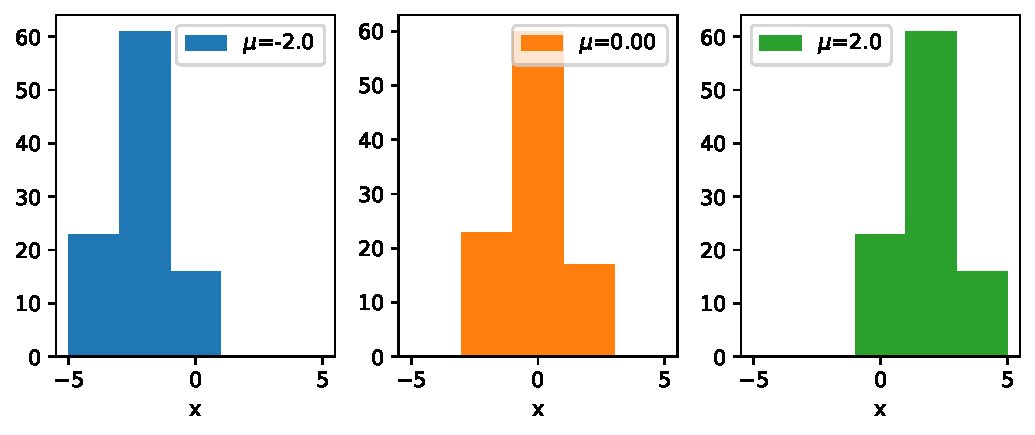
\includegraphics{./diffprog-hep_files/figure-pdf/fig-hist-mus-output-1.pdf}

}

\caption{\label{fig-hist-mus}Translating a histogram from left to right
by varying the center of the distribution the data is drawn from.}

\end{figure}

Let us now shift our focus to a single bin: we'll choose the bin
centered on 0, and monitor its height as we vary \(\mu\), shown in
Figure~\ref{fig-bin-height-mu}.

\begin{figure}

{\centering 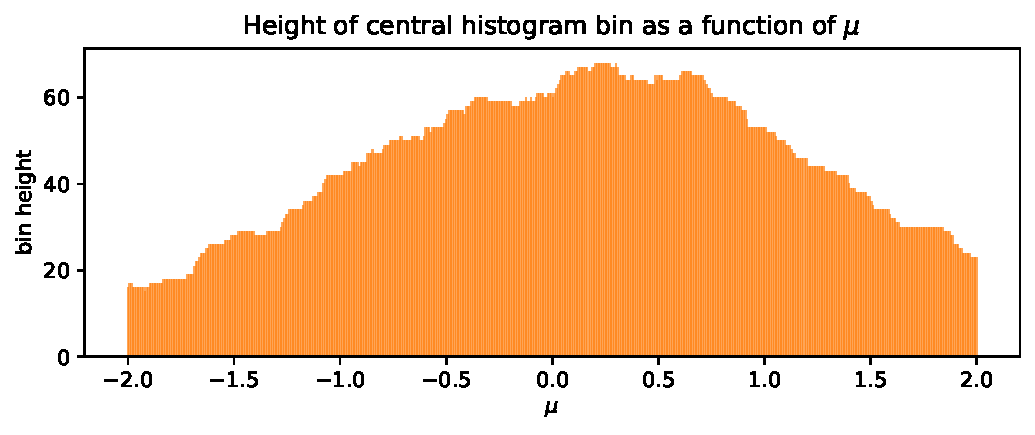
\includegraphics{./diffprog-hep_files/figure-pdf/fig-bin-height-mu-output-1.pdf}

}

\caption{\label{fig-bin-height-mu}Demonstrating the shift in the central
histogram bin as \(\mu\) is varied from -2 to 2.}

\end{figure}

We can see that the bin height jumps around in discrete intervals as we
translate the underlying data, which would produce ill-defined gradient
estimates if we used something numerical like finite differences. To
exploit the magic of automatic differentiation here, we want to make
some other function such that this envelope becomes smooth; varying
\(\mu\) by a very small amount should also vary the bin height by a
small amount instead of leaving it static or jumping discontinuously.

The solution that we developed to address this involves a \textbf{kernel
density estimate} (KDE). We discussed this in Section~\ref{sec-kde}, but
just to recap: a KDE is essentially the average of a set of normal
distributions centered at each data point, with their width controlled
by a global parameter called the \textbf{bandwidth}. There's a neat way
to take this and cast it into a bin-like form (i.e.~defined over
intervals): We can calculate the ``count'' in an interval by taking the
area under the KDE between the interval endpoints. We can do this using
the cumulative density function (cdf), as
\(P(a \leqslant X \leqslant b) = P(X \leqslant b) - P(X \leqslant a)\).
Since the KDE is the mean over some normal distributions, its cdf is
also just the mean of the cdfs for each normal distribution. Moreover,
to turn this into a histogram-like object, we can multiply the result by
the total number of events, which just changes the mean into a sum. We
put this all together in Figure~\ref{fig-bkde-code}, where a pseudocoded
implementation of a \textbf{binned KDE} (bKDE) can be found.

\begin{figure}
{\centering 

\begin{Shaded}
\begin{Highlighting}[]
\KeywordTok{def}\NormalTok{ bKDE(data: Array, bins: Array, bandwidth: }\BuiltInTok{float}\NormalTok{) }\OperatorTok{{-}\textgreater{}}\NormalTok{ Array:}
\NormalTok{    edge\_hi }\OperatorTok{=}\NormalTok{ bins[}\DecValTok{1}\NormalTok{:]  }\CommentTok{\# ending bin edges ||\textless{}{-}}
\NormalTok{    edge\_lo }\OperatorTok{=}\NormalTok{ bins[:}\OperatorTok{{-}}\DecValTok{1}\NormalTok{]  }\CommentTok{\# starting bin edges {-}\textgreater{}||}
    \CommentTok{\# get cumulative counts (area under kde) for each set of bin edges}
\NormalTok{    cdf\_hi }\OperatorTok{=}\NormalTok{ norm.cdf(edge\_hi.reshape(}\OperatorTok{{-}}\DecValTok{1}\NormalTok{, }\DecValTok{1}\NormalTok{), loc}\OperatorTok{=}\NormalTok{data, scale}\OperatorTok{=}\NormalTok{bandwidth)}
\NormalTok{    cdf\_lo }\OperatorTok{=}\NormalTok{ norm.cdf(edge\_lo.reshape(}\OperatorTok{{-}}\DecValTok{1}\NormalTok{, }\DecValTok{1}\NormalTok{), loc}\OperatorTok{=}\NormalTok{data, scale}\OperatorTok{=}\NormalTok{bandwidth)}
    \ControlFlowTok{return}\NormalTok{ (cdf\_hi }\OperatorTok{{-}}\NormalTok{ cdf\_lo).}\BuiltInTok{sum}\NormalTok{(axis}\OperatorTok{=}\DecValTok{1}\NormalTok{) }\CommentTok{\# sum cdfs over each kernel}
    \\
\end{Highlighting}
\end{Shaded}

\caption{ \label{fig-bkde-code}\textbf{Pythonic pseudocode for the implementation of a bKDE.}}

}



\end{figure}

\begin{figure}

{\centering 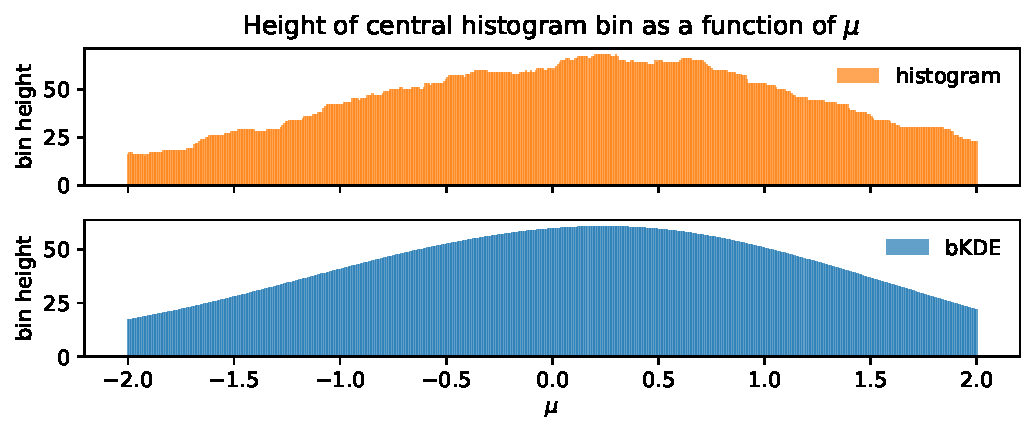
\includegraphics{./diffprog-hep_files/figure-pdf/fig-bin-height-bkde-output-1.pdf}

}

\caption{\label{fig-bin-height-bkde} Demonstrating the shift in the
central histogram bin as \(\mu\) is varied from -2 to 2 for both a
regular histogram and a bKDE.}

\end{figure}

Using this, we can remake the plot from Figure~\ref{fig-bin-height-mu}
for the bKDE, which we can see in Figure~\ref{fig-bin-height-bkde},
showing that the variation of the bin height with \(\mu\) is much more
well-behaved.

\hypertarget{choosing-the-bandwidth}{%
\subsubsection*{Choosing the bandwidth}\label{choosing-the-bandwidth}}
\addcontentsline{toc}{subsubsection}{Choosing the bandwidth}

I'll show a few studies here that illustrate what happens to the
accuracy of the bKDE histogram from the perspective of both the
distribution and the resulting gradients.

We know what happens to a KDE when we change the bandwidth: small
bandwidth gives a function with high variance, and a large bandwidth
oversmooths the distribution. How do these effects impact the bKDE? We
can quantify this \emph{relative to the bin width} by examining the
shape of the bKDE relative to a ``hard'' histogram, which is shown in
Figure~\ref{fig-bkde-bandwidth}. For low bandwidths, we recover
something almost resembling a regular histogram. In fact, in the limit
of zero bandwidth, we will \emph{exactly} get a histogram! The reason is
that zero bandwidth would turn each normal distribution into an infinite
spike at each data point, which, when integrated over to get the counts,
would have a contribution of 1 if the event lies in the bin, and 0
otherwise\footnote{For non-uniform bin widths, an extension of the bKDE
  to non-uniform bandwidths could be interesting -- one could keep the
  bin width/bandwidth ratio fixed for each bin, and if the event falls
  in a given bin, the resulting bandwidth from using that ratio is
  applied to that event. This would make the analogy between bin width
  and bandwidth more general in some ways, albeit at the cost of
  someone's coding time.}.

\begin{figure}

{\centering 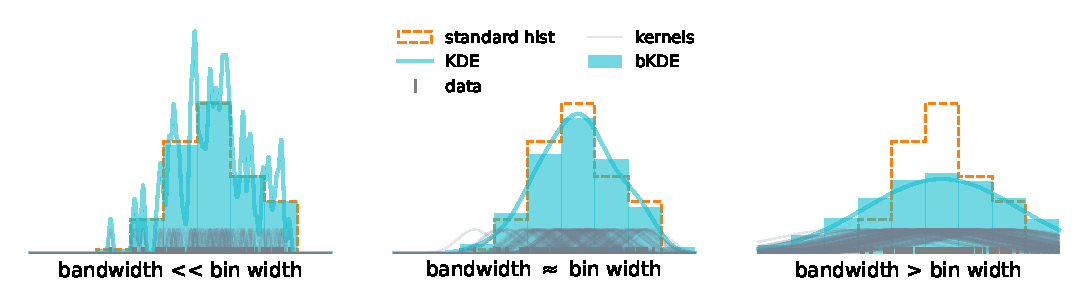
\includegraphics{./images/relaxed_hist.pdf}

}

\caption{\label{fig-bkde-bandwidth}Illustration of the bias/smoothness
tradeoff when tuning the bandwidth of a bKDE, defined over 200 samples
from a bi-modal Gaussian mixture. All distributions are normalized to
unit area. The individual kernels that make up the KDE are scaled down
for visibility.}

\end{figure}

This idea of a bias/variance tradeoff with the bandwidth is the gist of
it, but there's an additional factor that will influence the value of
the bandwidth chosen: the number of data samples available. We may
expect that as we add more samples to a KDE, there will be a lot more
kernels centered on the new points, so we'd want to reduce the bandwidth
in order to faithfully represent the envelope of the distribution. We
then can inspect the degree to which this also continues to hold for the
bKDE; it may be that good defaults for KDEs differ slightly compared to
those for bKDEs.

First, let's examine the distribution accuracy as a function of
bandwidth and number of data samples. We can define this by looking at
the ``true'' histogram, which can be calculated using the cumulative
distribution of \(\mathrm{Normal}(\mu, 1)\) in a way analagous to the
bKDE (i.e.~the integral under the curve over the intervals defined by
the bins), which we then normalize to the number of data samples
available. We can then plot the true height of the central bin as it
varies with \(\mu\), and compare it to that obtained from the histogram
and bKDE estimates across a number of different settings for the sample
size and bandwidth. These plots are shown in
Figure~\ref{fig-bin-height-all}, which looks at bandwidths of 0.05, 0.5,
and 0.8 in tandem with sample sizes of 20, 100, and 5000. As expected,
we see that the low bandwidth case has the histogram and bKDE
predictions for the bin mostly agreeing, while they diverge for larger
bandwidths. The best-case scenario appears to be when we have a large
number of samples and a low bandwidth, which is when we'd expect all
three estimates to converge. If we choose a bandwidth too large though,
we're going to introduce a bias as we oversmooth the data features.

\begin{figure}

{\centering 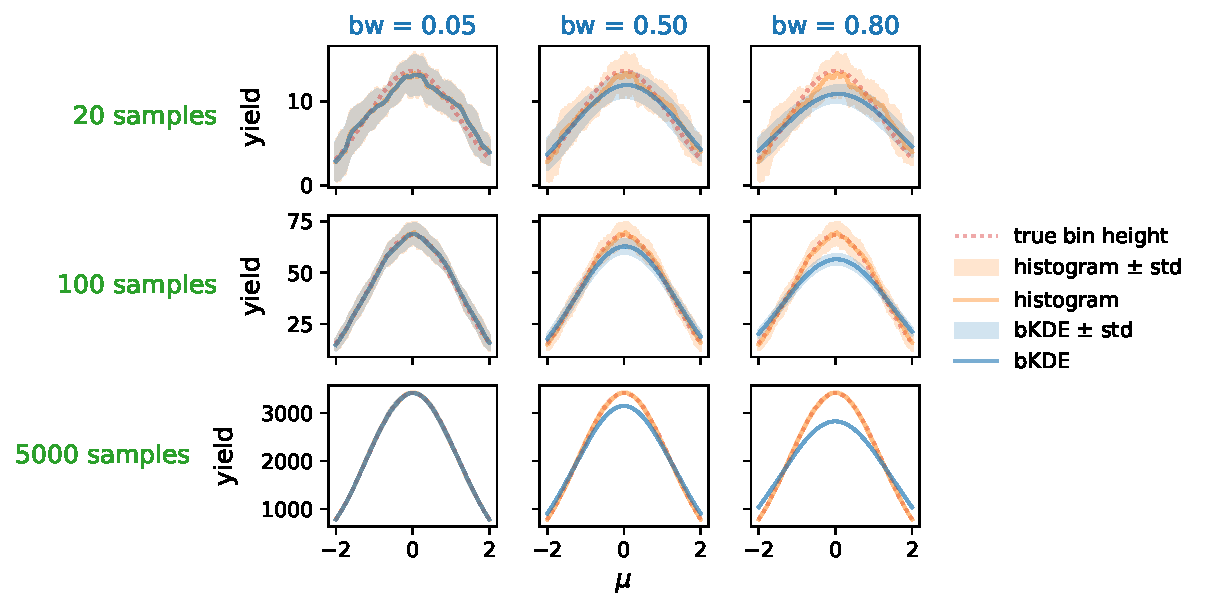
\includegraphics{./diffprog-hep_files/figure-pdf/fig-bin-height-all-output-1.pdf}

}

\caption{\label{fig-bin-height-all}Demonstrating the shift in the
central histogram bin as a function of bandwidth and the number of
samples for a histogram and bKDE, which are compared to the true bin
height.}

\end{figure}

So far things seem all to follow intuition somewhat, but we've only
checked half the picture; the whole reason we're using the bKDE
construct in the first place is so we can access \emph{gradients} of the
histogram yields. To study these, we can derive the ``true'' gradients
from the definition of the bin height: as before, a bin defined by
\((a,b)\) for a given \(\mu\) value is just

\[\operatorname{yield}_{\mathsf{true}}(\mu; a,b) = \Phi(b;\mu, \sigma) - \Phi(a;\mu, \sigma) ~,\]

where \(\Phi(x; \mu, \sigma)\) is the normal cumulative distribution
parametrized by \(\sigma, \mu\). We can then just take the gradient of
this expression with respect \(\mu\) by hand. First we write the
explicit definition of the cdf:

\[\Phi(x; \mu, \sigma) = \frac{1}{2}\left[1+\operatorname{erf}\left(\frac{x-\mu}{\sigma \sqrt{2}}\right)\right]~,\]

where the convenient short hand of the error function
\(\operatorname{erf}\) is given by

\[
\operatorname{erf}(x) \equiv \frac{2}{\sqrt{\pi}} \int_0^x e^{-t^2} d x~.
\]

Then, the derivative is as follows:

\[\frac{\partial}{\partial\mu}\Phi(x;\mu, \sigma) = \frac{1}{2}\left[1-\left(\frac{2}{\sqrt{2\pi}\sigma} e^{-\frac{(x-\mu)^2}{2\sigma^2}}\right)\right]~,\]

since
\(\frac{d}{dx} \operatorname{erf}(x)=\frac{2}{\sqrt{\pi}} e^{-x^{2}}\).

As mentioned, we have \(\sigma=1\) in this particular example, making
this expression simpler:

\[ \frac{\partial}{\partial\mu}\Phi(x;\mu, \sigma=1) = \frac{1}{2}\left[1-\left(\frac{2}{\sqrt{2\pi}} e^{-\frac{(x-\mu)^2}{2}}\right)\right]~.\]

Putting this all together gives us

\[\Rightarrow \frac{\partial}{\partial\mu}\operatorname{yield}_{\mathsf{true}}(\mu; a,b) = -\frac{1}{\sqrt{2\pi}}\left[\left(e^{-\frac{(b-\mu)^2}{2}}\right) - \left( e^{-\frac{(a-\mu)^2}{2}}\right)\right]~,\]

which we can use as a way to quantify the accuracy of the gradients
obtained from using a bKDE compared to those of the amount of the true
distribution in the interval \((a,b)\).

The comparative plots between the true gradient, the histogram gradient,
and the bKDE gradient are shown in Figure~\ref{fig-bin-grad-all}, where
the histogram gradient is calculated using the finite differences
method, and the bKDE gradient with automatic differentiation. A similar
trend can be seen to Figure~\ref{fig-bin-height-all}, where the estimate
from the bKDE improves with more samples, and becomes much less noisy.
This is in contrast to the histogram, which struggles with gradients
unless the sample size is large (here 5000), and produces very high
variance estimates in general. The bKDE, however, is able to avoid this
high variance while keeping a reasonably low bias depending on how many
samples are present; the central plot, for instance, shows a case where
the bKDE of bandwidth 0.5 far outperforms estimating the true gradient
with just 100 samples compared to the erratic estimates using the
regular histogram.

\begin{figure}

{\centering 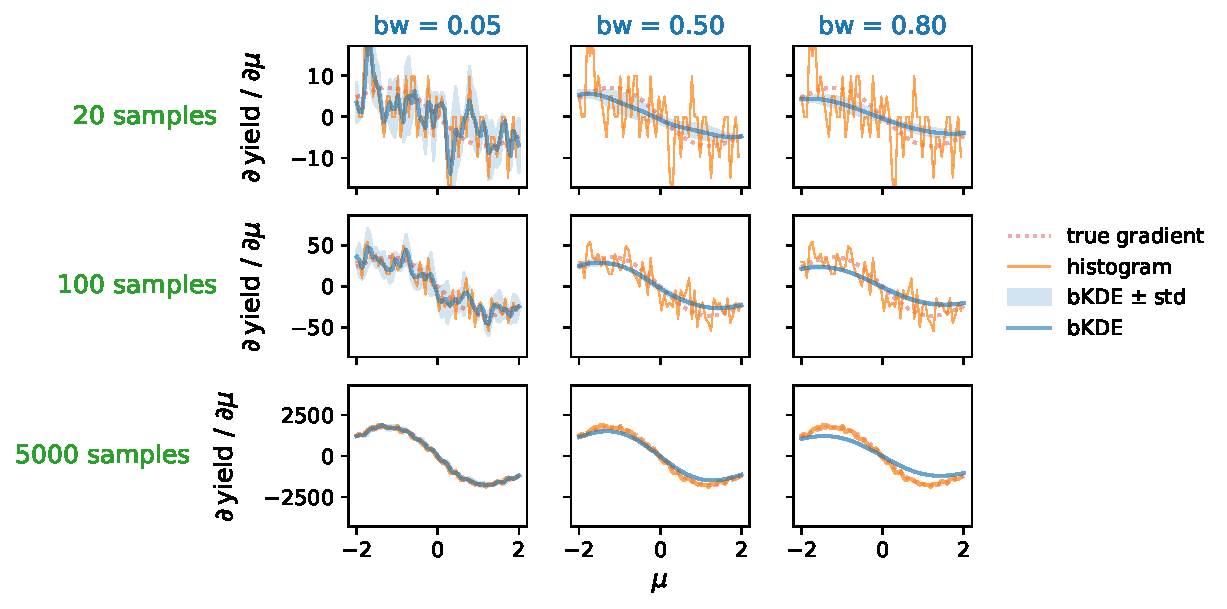
\includegraphics{./diffprog-hep_files/figure-pdf/fig-bin-grad-all-output-1.pdf}

}

\caption{\label{fig-bin-grad-all}Variation of the gradient of the
central histogram bin as a function of bandwidth and the number of
samples for a histogram and bKDE, which are compared to the true
gradient of the yield.}

\end{figure}

It seems then that there is some kind of middle ground to be had with
respect to the bandwidth one can choose for a bKDE depending on the
number of samples present, where the trends of distribution and gradient
accuracy roughly align. Optimality seems to be in the high-sample and
low-bandwidth case. To look at this at scale, we can summarize each of
these plots into a single number, e.g.~the mean relative error, and see
how this number varies across a large grid of different configurations
for the number of samples and the bandwidth. This plot can be found in
Figure~\ref{fig-grad-errors}, where a number of grid points are taken
for combinations of bandwidth/sample size, and the absolute relative
error in the gradient has been calculated (and averaged across three
random seeds, then a second averaging over 500 values of \(\mu\) in
(-2,2)). Orange scatter points are overlayed to show the bandwidth
choice that yields the minimum relative error given each of the studied
sample sizes. The trend is generally in agreement with that which we saw
in Figure~\ref{fig-bin-grad-all} of higher sample size letting us choose
lower bandwidths, but there's definitely a little pause for thought
given the couple points that deviate from forming a neat straight line.
There also appears to be a little pocket of lower error around 2000
samples, which doesn't appear to have any obvious explanation. Given
more time, one could study this in detail with a much finer grid (memory
and temporal limitations prevented expanding this further), and for a
variety of different examples, then maybe perform
\href{https://github.com/MilesCranmer/PySR}{symbolic regression} to
infer a good rule of thumb. This could also be recasted into a rule of
thumb relative to the bin width, which could be a useful metric for
comparison (e.g.~in Figure~\ref{fig-bkde-bandwidth} shown earlier).

\begin{figure}

{\centering 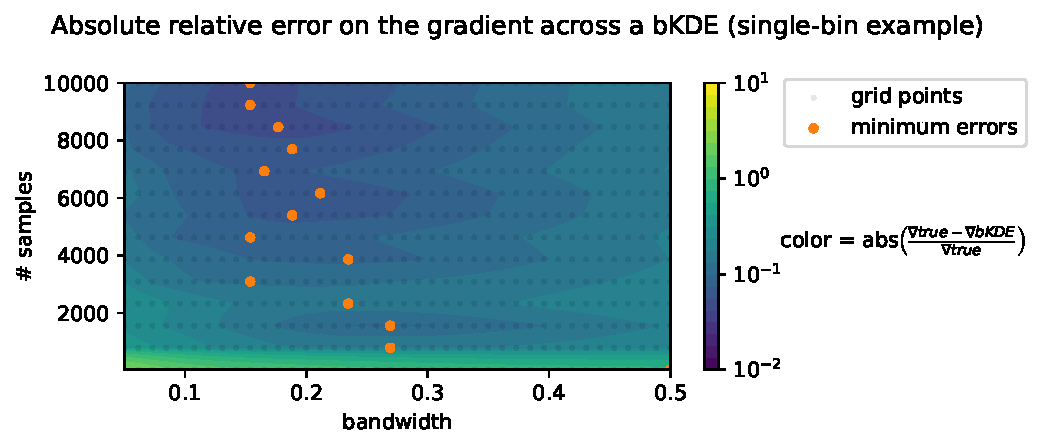
\includegraphics{./images/grad_errors.pdf}

}

\caption{\label{fig-grad-errors}Absolute relative error in the bKDE
gradient compared to the true distribution, calculated for a wide
variety of bandwidths and sample sizes. Orange points indicate the
lowest error across the rows of constant sample size to hint at the
trend of a good bandwidth choice.}

\end{figure}

\hypertarget{other-differentiable-binned-density-estimates}{%
\subsubsection*{Other differentiable binned density
estimates}\label{other-differentiable-binned-density-estimates}}
\addcontentsline{toc}{subsubsection}{Other differentiable binned density
estimates}

In the INFERNO paper (Castro and Dorigo 2019), from which much
inspiration was taken in general, they use a softmax function as a way
to mimic binned output from the neural network, which would have an
output dimensionality equal to the number of bins you want in your
histogram. We can then think about each data point having a weight of 1,
and having the softmax smoothly distribute that weight across the
different bins. For a dataset \(\mathbf{x}\) and a fixed neural network
\(\mathbf{y}\) with output nodes \(y_i\) up to \(y_N\), the yield of bin
\(i\) in the histogram is calculated by summing the softmax
contributions from each data point in that bin:

\begin{align}
\text{softmax histogram}_{\text{bin } i}(\mathbf{x}) &= \sum_{\text{data }k} \text{softmax}(x_k, y_i) \\
&= \sum_{\text{data }k} \frac{e^{y_{i}(x_k) / \tau}}{\sum_{j=0}^{\text{N}} e^{y_{j}(x_k) / \tau}}~,
\end{align}

where \(\tau\) is a factor to tune how hard the slope of the softmax is,
i.e.~it has some analogy to the bandwidth about tuning the level of
approximation. A drawback, however, is that the softmax used in tandem
with a neural network does not come with an inherent notion of
\emph{ordering}; it's going to be somewhat arbitrary in which bins
events occupy, and the resulting plots are a little hard to interpret
compared to regular histograms. Also, even the ``hard'' softmax with
\(\tau \rightarrow \infty\) is difficult to map to some other ``true''
histogram in which the bins follow Poisson-distributed counts.

As for other things, one could always do something like overlap sigmoid
functions, or even make a KDE with a new histogram-like kernel. We'll
cap our imagination here though, and move onwards to the likelihood that
this histogram is part of.

\hypertarget{differentiable-likelihood-construction}{%
\subsection{Differentiable likelihood
construction}\label{differentiable-likelihood-construction}}

Now, I must confess, I have told you a bit of a white lie to set up the
motivation here. The likelihood function as described in
Equation~\ref{eq-hifabase} is indeed a-priori differentiable with
respect to the histograms that make up the expectations. The problem is
actually a \emph{technical} one -- we need to make this happen in code.
As per our conversations on automatic differentiation, we know how to do
this: we code up our program using a framework for automatic
differentiation that has defined primitives and gradient rules.
\texttt{pyhf} Heinrich et al. (2021) is the software package that brings
this to life: the whole HistFactory prescription, all coded using a
choice of autodiff backends, e.g.~JAX, TensorFlow, and PyTorch. There's
honestly not too much else to say here; any further discussion would
involve extremely niche and technical topics within the \texttt{pyhf}
codebase, and all the error messages I saw over the years I worked on
trying to hack things together. I'll spare you that discussion (feel
free to ask about it, or
\href{https://github.com/scikit-hep/pyhf/issues?q=is\%3Aissue+author\%3Aphinate+}{browse
the \texttt{pyhf} issues on the topic}), and we'll move on to something
a little more thesis-suited (though, what is a PhD if not niche and
technical\ldots).

\hypertarget{differentiable-test-statistics-profile-likelihood-ratio}{%
\subsection{Differentiable test statistics (profile likelihood
ratio)}\label{differentiable-test-statistics-profile-likelihood-ratio}}

Recall from Section~\ref{sec-asymptotics} that when we're constructing
test statistics, we're using the building block of the \emph{profile
likelihood ratio}, which we state once again as

\[
\lambda(x, \mu) = \frac{p\left(x|\mu,\hat{\hat{\theta}}(\mu)\right)}{p\left(x| \hat{\mu}, \hat{\theta}\right)}~.
\]

The variables \(\hat{\hat{\theta}}(\mu)\) and
\(\hat{\mu}, \hat{\theta}\) are the result of two separate maximum
likelihood fits. Are these differentiable? Well, yes -- we can leverage
the utility of automatic differentiation to trace each iteration of the
optimization loop at runtime, and then do the corresponding gradient
calculation by composing VJPs and the like. However, that could get
really expensive as the number of iterations gets into the thousands,
which isn't too uncommon in practice. Do we have a way to get around
this?

Thanks to the groundwork we set up in Section~\ref{sec-fixed-points}, we
worked out that we can take the gradient of \textbf{fixed points}
(e.g.~solutions to minimization algorithms) through a simple analytic
formula in terms of the update step \(f\), the solution of the
optimization problem \(\theta_0\) (or \(\hat{\theta}\)), and some
particular value of \(\varphi=\varphi_0\) that we used to define the
objective:

\begin{equation}\protect\hypertarget{eq-fixed-point}{}{
\frac{\partial\theta_0}{\partial\varphi_0}= \left[I - \frac{\partial f}{\partial \theta_0} \right]^{-1} \frac{\partial f}{\partial \varphi_0}~.
}\label{eq-fixed-point}\end{equation}

What does \(\varphi\) mean here? It corresponds to the \emph{same}
\(\varphi\) that we're talking about in this section (the notation was
not a coincidence)! Specifically, these would be the \emph{analysis
configuration parameters} (e.g.~a combination of neural network
parameters, observable binning, cutflow, etc.), which all
\emph{implicitly} determine the form of the likelihood. The language of
``implicit'' refers to the fact that we build the likelihood using the
counts of the histograms for each physics process, with those counts in
turn being influenced by \(\varphi\), but we do not explicitly denote
the likelihood as \(p(x|\mu, \theta, \varphi)\), for instance.

In practice, we can implement this through moving the goalposts for what
we call a primitive: for optimization loops like this, we can define
that as a primitive of sorts, and then give it the known gradient as
defined by Equation~\ref{eq-fixed-point}. This is the kind of approach
taken by \texttt{jaxopt} (Blondel et al. 2021), which is a library
that's used a few times in this thesis.

\hypertarget{differentiable-hypothesis-tests}{%
\subsection{Differentiable hypothesis
tests}\label{differentiable-hypothesis-tests}}

What's left to get us over the line to differentiating the result of a
hypothesis test? Well, thanks to the formulae outlined in
Section~\ref{sec-asymptotics}, to extract the expected (read: median)
\(p\)-value from the observed value of the test statistic \(t(x_0)\), we
only need to do one last simple algebraic calculation:

\begin{itemize}
\tightlist
\item
  For the \textbf{discovery \(p\)-value} with test statistic \(q_0\):
  \(p_0 = 1-\Phi(\sqrt{q_0})\).
\item
  For the \(p\)-value associated with setting an \textbf{upper limit}
  using test statistic \(q_\mu\): \(p_\mu = 1-\Phi(\sqrt{q_\mu})\).
\item
  For the \(\text{CL}_s\) \textbf{method}, we can just compose the
  \(p\)-values from the previous step using different values of \(\mu\)
  in \(q_\mu\) as the point null:
  \(\text{CL}_s = p_{\mu=1} / (1-p_{\mu=0})\).
\end{itemize}

All of these formulae are differentiable without any extra work, so
we're done!

\hypertarget{sec-inferno}{%
\subsection{Bonus: Uncertainties on likelihood
parameters}\label{sec-inferno}}

Recall from Section~\ref{sec-fisher} that the \emph{Fisher information
matrix} \(\mathcal{I}(\theta)\) gives us access to the covariance matrix
for maximum likelihood estimates, provided we're in the asymptotic
limit, through the Cramér--Rao bound:

\[
\Sigma_{\hat{\theta}}^{2} \geqslant [\mathcal{I}(\theta)]^{-1}~.
\]

Since \(\mathcal{I}(\theta)\) is defined in terms of second-order
derivatives of the log-likelihood -- something that we've already made
differentiable from a code perspective -- we can then calculate the
Fisher information using automatic differentiation. Moreover, since
function transformations like the gradient operator are composable in
automatic differentiation frameworks, this will itself be
differentiable! This gives us access to many other inference-aware
quantities that we can use as both diagnostics and as loss functions,
including diagonal elements of the covariance matrix, which correspond
to the individual uncertainties on each likelihood parameter. This
approach was first explored by INFERNO (Castro and Dorigo 2019), from
whom we take much inspiration from in this section.

Now, the Fisher information involves a matrix filled with second
derivatives of the likelihood, and so requires data and parameters to be
evaluated as a number. One thing we can do in the HistFactory setting is
use Asimov data, which would mean we'll be able to know the best-fit
parameter values already, and we can attempt to achieve the Cramér--Rao
bound in Equation~\ref{eq-cramer-rao} by evaluating at \(\mu=\mu'\),
\(x=x_A(\mu')\). As to the choice of \(\mu'\), I'm not sure that it
matters too much, as we're always going to be at the best fit parameter
value for \(\mu\) (the likelihood shape itself isn't affected by this,
for instance), but I haven't studied this in detail.

\hypertarget{putting-it-all-together}{%
\section{Putting it all together!}\label{putting-it-all-together}}

Now that we've enabled the differentiability of all the components layed
out in Equation~\ref{eq-neos}, we can see what happens when we use use
the \(p\)-value as out loss function, i.e.~use gradients in
Equation~\ref{eq-analysis-chain-rule} to update the parameters
\(\varphi\).

As a first example, we can look at the simple analysis from
Section~\ref{sec-simple-anal} as a candidate to test this out on! We
were looking for the value of \(\phi\) that corresponds to the best
expected sensitivity to the signal model. Crucially, we needed to make
sure that we accounted for the systematic uncertainty on the background
\(\sigma_b\), which heavily influenced the resulting optimization. Let's
see if we can do that!

The results of training this setup to optimize \(\phi\) with respect to
the discovery \(p\)-value can be seen in Figure~\ref{fig-simple-opt}.
Immediately, we can see that we've managed to find a point that
minimizes the objective we care about, being able to incorporate
uncertainty all the while! One thing I really like about this plot is
the way it appeals to intuition -- the expected counts that result from
this procedure appear to be exactly at some medium compromise between
signal to background ratio and uncertainty on the background. The
acquired Swede within me would even go as far as to call it ``lagom'' --
not too little, not too much; just the right amount\footnote{If you're
  less of a holistic person and would prefer something more
  quantitative, you can see a real-life carving of the ``lagom'' amount
  in Lund, just outside one of the main university buildings.}.

\begin{figure}

{\centering 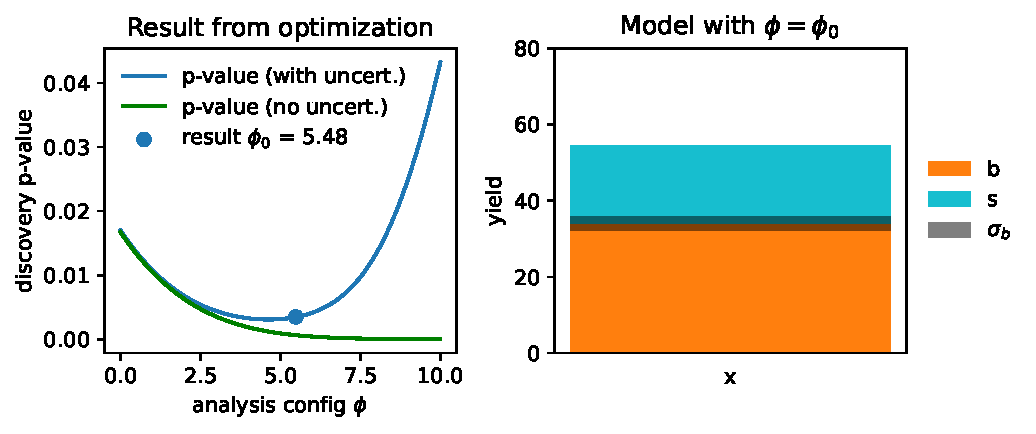
\includegraphics{./images/opt.pdf}

}

\caption{\label{fig-simple-opt}Left: The resulting point from optimizing
\(\phi\) with gradient descent. Right: The histogram model at the
solution of the optimization.}

\end{figure}

\hypertarget{a-quick-aside-on-inferno-vs-neos}{%
\subsection{\texorpdfstring{A quick aside on INFERNO vs
\texttt{neos}}{A quick aside on INFERNO vs neos}}\label{a-quick-aside-on-inferno-vs-neos}}

My advocacy hereafter is to refrain from using \texttt{neos} or INFERNO
methodology naming, since these methods differ only on small
implementation details, the main one being the \emph{choice of loss
function}.

But while we're comparing them, there's one interesting thing to note: we're calculating the expected discovery
\(p\)-value using the asymptotic formulae outlined in
Section~\ref{sec-asymptotics}. Minimising this \(p\)-value corresponds
to pushing the observed value of the \(q_0\) test statistic as far to
the right as possible (i.e.~maximizing its value), which will trap
smaller and smaller proportions of the distribution \(p(q_0 | \mu_0)\)
(smaller \(p\)-values). Recall that Equation~\ref{eq-wald} states that
we know an interesting fact about this test statistic: it's
approximately equal to
\(\left((\mu_0 - \hat{\mu}(x))/\sigma_{\hat{\mu}}\right)^2\). Since
we're using Asimov data with \(\mu'=\hat{\mu}=1\), and probing a null of
\(\mu_0=0\), the test statistic is actually an (inverse) estimate of the
variance of \(\hat{\mu}\), which is being minimized during optimization!
This has a lot of similarities with INFERNO, since both methods are
effectively minimizing the same quantity, but estimated a different way;
INFERNO uses the Fisher information estimate, and \texttt{neos} uses
asymptotic formulae.

If we were to apply this same logic to calculating a \(p\)-value (or a
\(\mathrm{CL}_s\) value) for upper limit setting, then we'd insead be
using \(q_\mu\), and would typically examine Asimov data with
\(\mu'=\hat{\mu}=0\) (no signal) while looking at a null of \(\mu_0=1\).
We would then still end up with the same relation of inverse
proportionality to \(\sigma_{\hat{\mu}}^2\). Of course, the test
statistics \(q_0\) and \(q_\mu\) differ conceptually in their
definition, so there are likely going to be differences in practice if
we used one or the other for optimization (but we would definitely
expect a reduced uncertainty on \(\hat{\mu}\) in either case). We'll see
these differences in practice later on.

Equipped with these systematic-aware (or more aptly,
\emph{inference}-aware) loss functions, we can now apply them to
something a little more complicated.

\hypertarget{sec-neos}{%
\section{\texorpdfstring{\texttt{neos}: End-to-End Optimized Summary
Statistics for High-Energy
Physics}{neos: End-to-End Optimized Summary Statistics for High-Energy Physics}}\label{sec-neos}}

This section summarizes the work I've done in the paper (Simpson and
Heinrich 2021). New follow-up studies will be shown in later sections.

The problem of reducing a whole set of physics quantities into a single
number, or \textbf{summary statistic}, is not a new one in HEP. The
reason for this is two-fold: inference in high-dimensional settings is
computationally difficult, and the probability model defined by the
underlying physics is intractable to explicitly compute. This leads to
practice referenced a few times already, where we construct models via
HistFactory, which are almost always based a single quantity,
e.g.~something like the invariant mass of the final state you're
interested in, or the output of a machine learning model. In the latter
case, we're typically concerned with optimizing for discriminating
signal and background processes. However, we know from the previous
sections that we can do much better by optimizing with respect to a
\(p\)-value, especially when we have significant systematic
uncertainties to worry about.

To be more concrete: we'll look at optimizing a neural network-based
summary statistic for a simple HEP-like situation, including the
construction of the uncertainty through interpolating between ``up'' and
``down'' variations of the background. We'll refer to this workflow as
\texttt{neos}\footnote{Originally an acronym for neural end-to-end
  optimized statistics, but acronyms are annoying, so I don't really
  make that explicit anymore. Hopefully the rest of this section will
  also convince you that we don't need to get too caught up with naming
  anyway.}, with the full proposed pipeline shown in
Figure~\ref{fig-neos}.

\begin{figure}

{\centering 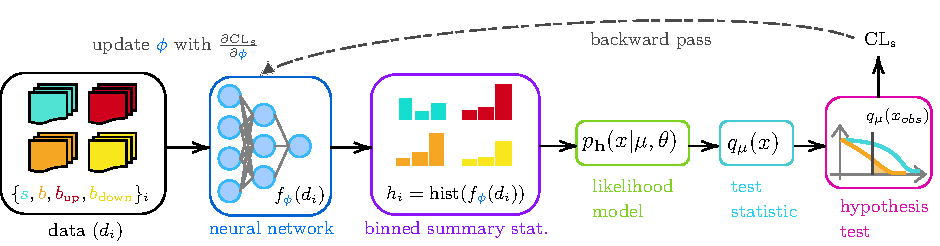
\includegraphics{./images/neos.pdf}

}

\caption{\label{fig-neos}Outline of the workflow proposed for
\texttt{neos}.}

\end{figure}

\hypertarget{example-gaussian-blobs}{%
\subsection{Example: Gaussian blobs}\label{example-gaussian-blobs}}

Pretending our detector only outputs two physics variables \(x\) and
\(y\), we'll generate some toy data from different 2-D normal
distributions (``Gaussian blobs'') for both signal and background,
making sure they overlap a bit as to not be trivially separable. We'll
then also sample from Gaussian blobs on either side of the background,
and treat these as ``up'' and ``down'' variations in the way described
in Section~\ref{sec-hifa-nps}. We can see the result of sampling 10k
points for each blob in Figure~\ref{fig-data-space}.

\begin{figure}

{\centering 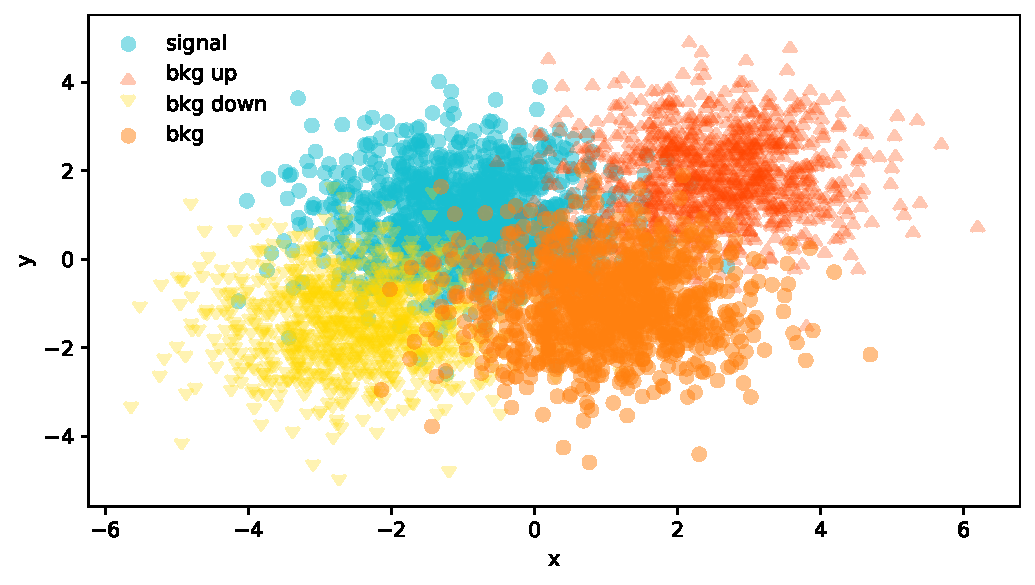
\includegraphics{./images/data-space.pdf}

}

\caption{\label{fig-data-space}Plot of 10k samples from toy
distributions representing imagined signal, background}

\end{figure}

From here, things follow the diagram in Figure~\ref{fig-neos}:

\begin{itemize}
\tightlist
\item
  We'll pass the samples of \(x, y\) values for each blob through a
  neural network, which turns each tuple of \((x, y)\) into a single
  number \(f_\varphi(x, y)\), where \(f_\varphi\) is our current network
  with parameters \(\varphi\).
\item
  We'll then have four sets of values of \(f_\varphi\) for each blob
  (signal, nominal background, and the up and down variations of the
  background), which we then turn into four histograms. During
  optimization, this histogram will be a bKDE as per
  Section~\ref{sec-bkde} to make the final loss (\(\mathrm{CL}_s\))
  differentiable, but we'll replace it with a regular histogram for
  calculating our evaluation metrics.
\item
  Using these histograms, we'll build a HistFactory statistical model in
  exactly the same fashion as Equation~\ref{eq-simplemodel} -- with one
  parameter for the signal strength \(\mu\), and one nuisance parameter
  \(\gamma\) that's constructed by interpolating the shape variation
  between the histograms of the nominal, up, and down variations of the
  background.
\item
  We then build the appropriate test statistic based on this likelihood,
  and perform our hypothesis test -- not on the observed data (we don't
  have any), but on the Asimov dataset for that hypothesis (i.e.~for a
  null of \(\mu=1\), we're going to use the dataset that would result in
  \(\hat{\mu} = 1\) when fitting the likelihood, which would just be the
  nominal counts \(s + b\)).
\item
  The final step is producing the end result of that test
  (e.g.~\(\mathrm{CL}_s\)), then taking the gradient of that whole
  chain, which we'd use to update the parameters of the neural network
  \(\varphi\).
\end{itemize}

We'll feed data in using mini-batches, and hold out a group of points
for each blob as a test set, which we use to calculate metrics and
select the best model (normally we should never use the test set to
choose a model, but the distributions are simple enough that there will
be almost no macroscopic difference between train, validation, and test
sets). The histogram yields are all divided by the number of data points
per-batch, and then re-scaled to be on the order of tens of events, with
different factors being applied to signal and background to put us in a
more realistic regime (e.g.~of low signal and high background).

In the graphs about to be shown, we'll benchmark \texttt{neos} against
optimization against some other loss functions:

\begin{itemize}
\tightlist
\item
  \textbf{Binary cross-entropy} (BCE): This will try to discriminate
  signal versus nominal background samples, and will not be informed
  about the up/down samples during training.
\item
  \textbf{BCE with data augmentation}: As above, but we indiscriminately
  label all of the background samples with one label instead of using
  just the nominal (this should be a very powerful baseline).
\item
  \textbf{INFERNO}: As in Section~\ref{sec-inferno}, we'll take our loss
  to be the diagonal element of the inverse Fisher information that
  corresponds to the signal strength \(\mu\).
\end{itemize}

\hypertarget{results-as-shown-in-the-neos-paper}{%
\subsubsection*{\texorpdfstring{Results (as shown in the \texttt{neos}
paper)}{Results (as shown in the neos paper)}}\label{results-as-shown-in-the-neos-paper}}
\addcontentsline{toc}{subsubsection}{Results (as shown in the
\texttt{neos} paper)}

The full set of hyperparameters for this study are:

\begin{itemize}
\tightlist
\item
  10000 data points, split evenly between all four blobs,
\item
  3-layer neural network of size (1024, 1024, 1),
\item
  Training with Adam optimiser, learning rate 1e-3,
\item
  Adam optimiser also used in maximum likelihood fits with learning rate
  1e-3,
\item
  \(m_\mathrm{s}=(-1, 1)\), \(m_\mathrm{b}=(2.5, 2)\),
  \(m_\mathrm{bup}=(-2.5, -1.5)\), \(m_\mathrm{bdown}=(1, -1)\),
\item
  Multiplicative histogram scale factors: signal scale=2, background
  scale=10, global scale=10,
\item
  ReLU activations, with sigmoid activation on the final layer,
\item
  15 epochs, with a batch size of 2000.
\end{itemize}

Results from the training process using these hyperparameters are shown
in Figure~\ref{fig-neos-results}, where each curve is the average of
that metric across 7 different training runs, all with unique random
initializations of the neural network parameters. The figure has three
plots, which we'll cover from left to right. Note: these quantities are
all computed on the same \emph{test set} (unseen data), and use no
approximations to hard operations in their calculation (which basically
means the histogram is a normal one for \texttt{neos} and INFERNO).

\begin{figure}

{\centering 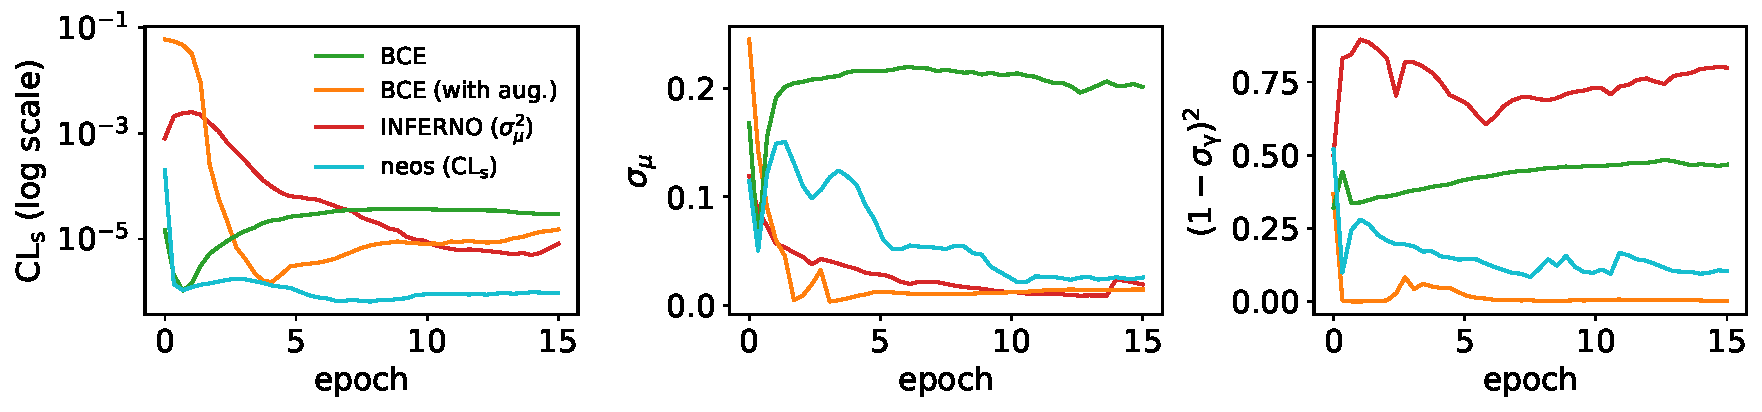
\includegraphics{./images/neos-results.pdf}

}

\caption{\label{fig-neos-results}Results from training neural networks
using the four loss functions highlighted in the legend. Left: the
expected \(\text{CL}_s\). Middle: The uncertainty on the signal strength
\(\mu\). Right: The deviation from the nominal width of the nuisance
parameter \(\gamma\) that controls the background uncertainty.}

\end{figure}

The leftmost plot contains the expected \(\mathrm{CL}_s\) for all four
methods. We can see that the absolute lowest value of this is only
attained by \texttt{neos}, which makes sense -- we're using this as the
loss function itself. Both BCE methods reach a fairly low value quite
quickly, which can be attributed to the fact that it's not that
difficult to isolate most of the signal in this example. Interestingly,
INFERNO demonstrated far less stability with it's \(\mathrm{CL}_s\)
value, with the different training runs having quite large variance in
this quantity, causing their average to perform quite poorly. This says
more about the interplay between the uncertainty on the signal strength
and the \(\mathrm{CL}_s\) than it does about what we consider ``good
performance'' -- I'll come back to this in the discussion.

The middle plot is the uncertainty on the fitted value of the signal
strength \(\sigma_{\hat{\mu}}\), as calculated through the Fisher
information. Something I think is cool here is that \texttt{neos} learns
to minimize this over time without any explicity prompting to do so
(we'll discuss more on this later). It's no surprise that INFERNO does
very well here, as again, it's trained precisely to do so. BCE with
augmentation also does very well, which is likely because we've ensured
that anything that is non-signal looking, including possible variations
on the background, is pushed to one side of the histogram, and the
signal, which can be well isolated, is pushed to the other. Regular BCE,
however, does okay initially, but will quickly overfit to the nominal
signal/background discrimination if left to train for longer, which
won't care if there's high background uncertainty in the signal bins.

The final plot on the right shows the squared deviation from the nominal
uncertainty on the background nuisance parameter \(\gamma\), which we
acquire through the appropriate diagonal term in the inverse Fisher
information. In the likelihood modelling stage, this uncertainty also
has an associated constraint term of \(\mathrm{Normal}(0 | \gamma, 1)\),
where the ``units'' of \(\gamma\) are chosen such that
\(\gamma_{\mathrm{nom}}\) sits at 0, and
\(\gamma_{\mathrm{up}}/\gamma_{\mathrm{down}}\) lie at +/- 1
respectively. If the standard deviation of the fitted value
\(\hat{\gamma}\) is different to 1, we then have a contradiction between
the fitted model and the implied uncertainty from the constraint term.
This is known as over/under-constraining the parameter (depending if the
uncertainty is smaller/bigger than 1), and can be associated with model
misspecification (although there are cases where it is perfectly
reasonable to constrain the nuisance parameter depending on the nature
of the measurement). Plotting this term (or
\((1-\sigma_{\hat{\gamma}})^2\) to just show the deviations) is then a
useful diagnostic to see the learned behaviour of the observable with
respect to the nuisance parameter. Training with \(\mathrm{CL}_s\)
doesn't appear to introduce any pathologies in this regard, and in fact
appears to further reduce dissonance between the constraint term and the
Fisher information with more training. This is also the case for BCE
with augmentation, but vanilla BCE and INFERNO don't appear to exhibit
this behaviour, and instead show some differences with the modelled
standard deviation. The fact that BCE has no awarness of the background
variations makes this less surprising, but I understand this less well
for INFERNO at the time of writing (or even if it's a problem at all).

\hypertarget{sec-neos-issues}{%
\subsection{Practical issues}\label{sec-neos-issues}}

Regardless of any results, one immediate concern that you may have
thought of while I talked about \texttt{neos} was the scaling aspect. We
can't escape that one forward pass and one update step is
computationally equivalent to two runs of the whole analysis inference
chain (rembembering that gradients from autodiff are of the order of the
forward pass to calculae). In practice, this seemed to be around
\textasciitilde3-4x an increase in performance time for an update to
complete compared to BCE, but I'd expect this to increase more when
applied to real analyses due to the complexity of the model, which has
to be built each time for every set of new parameters\footnote{I did
  some work on trying to cache these models and update them in-place --
  if you're interested, see
  \href{https://github.com/scikit-hep/pyhf/issues/1894}{this
  \texttt{pyhf} issue}}, and also will have a much larger number of
parameters, which will impact the speed of calculating the profile
likelihood.

Another issue is that these inference-aware metrics require enough data
to produce a reasonable reflection of the actual analysis model. With a
very small batch size, this is impossible; for medium-size batches, it
may be that some kind of proportional scaling needs to occur so the
yields maintain the same relative sizes, as was done in practice during
the Gaussian blobs example (not using these scale factors actually makes
trainining unstable).

\hypertarget{whats-really-the-best-loss-function}{%
\section{\texorpdfstring{What's \emph{really} the best loss
function?}{What's really the best loss function?}}\label{whats-really-the-best-loss-function}}

The work done in making \(\mathrm{CL}_s\) differentiable opened up a
variety of new inference-aware losses as a by-product, including but not
limited to:

\begin{itemize}
\tightlist
\item
  \(\mathrm{CL}_s\) (and its associated \(p\)-values)
\item
  \(p\)-value for discovery (\(p_0\))
\item
  Quantities derived from the Fisher information matrix of the full
  HistFactory likelihood, such as:

  \begin{itemize}
  \tightlist
  \item
    uncertainty on the signal strength \(\sigma_{\mu}\)
  \item
    deviations from the nominal nuisance parameter uncertainty,
    e.g.~\((1-\sigma_{\hat{\gamma}})^2\)
  \item
    the generalized variance, defined as the inverse determinant of the
    Fisher information
  \end{itemize}
\item
  Deviations from the nominal values of the nuisance parameters from
  control measurements (``pulls'')
\item
  \ldots and \emph{any algebraic combination of the above!}
\end{itemize}

Indeed, since all of these quantities can be calculated in a
differentiable way, we can create a hybrid loss function using any of
these components, such as
\(a_1 \mathrm{CL}_s + a_2\sigma_{\mu}^2 + a_3\log{p_0} + \dots\) etc. We
can even view this through the lens of regularization, where we have one
clear loss target, then introduce other components weighted with small
linear coefficients to steer away from potentially undesirable
pathologies.

Amongst those metrics already mentioned, one further example of a
quantity that could serve this purpose is the empirical notion of the
``\textbf{Gaussianity}'' of a likelihood, which my colleague/supervisor
Lukas Heinrich coined as the mean-squared difference across a grid of
points between the learned HistFactory likelihood and a Normal
distribution defined using the covariance implied by the (inverse)
Fisher information matrix (remember the Cramér--Rao bound from
Section~\ref{sec-fisher}). This would essentially control the validity
of the assumptions made when using the Fisher information to calculate
uncertainties, as well as potentially reducing the chances of arriving
at poorly-behaved likelihood shapes that happen to satisfy a low value
of any particular metric.

But despite all of this, I find myself a little bit torn as to the real
answer to the question posed in the section title: which loss function
is \emph{really} the best for physics analysis? This inquiry brings us
one layer deeper philisophically, as it touches on a more delicate
question: how do we actually gauge how good a physics result is? We'd
maybe say something that aligns with our physics goals, e.g.~the
discovery significance, but the way we assess analyses is a little more
nuanced than this in reality. One can see this by thinking about
reviewing an analysis paper -- we're not just interested in the
significance alone, but also things like the pull plots, the validity of
the modelling assumptions, whether things are correlated in the right
place, and probably many other things that I'm not thinking of.
Moreover, these nuances would be even \emph{more} important if the
significance was high!

As a very preliminary exploration of this question, we'll look at an
example problem where the ``best'' solution is clear. We can then
attempt to construct a loss function that is convex in the region of the
optimum.

\hypertarget{sec-which-loss-model}{%
\subsection{A loss landscape interlude for a two-bin
model}\label{sec-which-loss-model}}

The problem we'll look at is as follows: similar to the Gaussian blob
problem, we'll define a two-bin HistFactory model with a signal strength
\(\mu\) and a three-point uncertainty on the background \(\gamma\). This
model will be constructed from fixed nominal signal and background
yields of \(s = [5, 11]\) and \(b = [50, 50]\), with two free parameters
\(u\) and \(d\) that control the up and down variations:
\(b_{\mathrm{up}} = [50 + u, 50 -u ]\),
\(b_{\mathrm{up}} = [50 - d, 50 + d ]\). The intuition for this is that
any change in \(u\) or \(d\) will asymmetrically affect each bin by the
same amount, so any optimization can't focus on the gains from just one
of the two bins. When both \(u\) and \(d\) are equal to 0, we'll have
\(b = b_{\mathrm{up}} = b_{\mathrm{down}}\), i.e.~no systematic
uncertainty on the background. We know that this would be the ideal
solution, but what do our metrics have to say about it?

\begin{figure}

{\centering 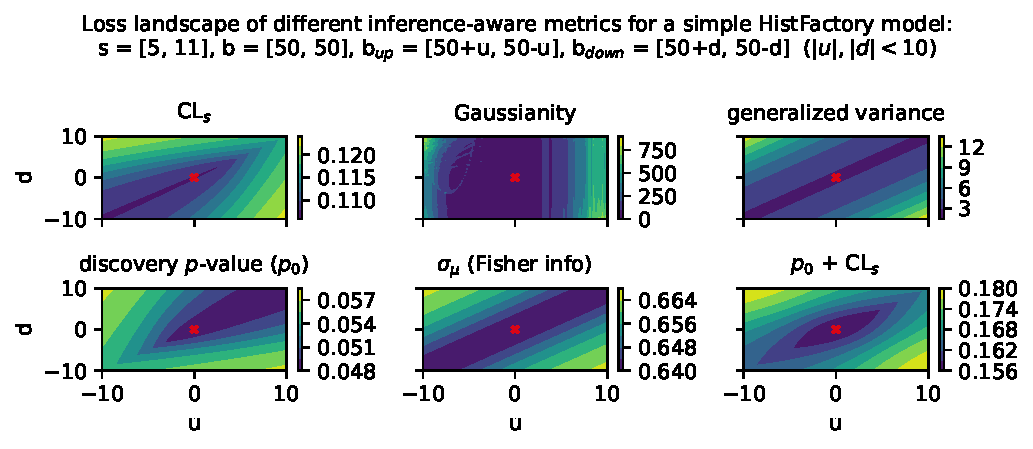
\includegraphics{./images/metrics-title.pdf}

}

\caption{\label{fig-whichloss}A scan over the loss landscape for a
two-parameter physics model, with each parameter having an asymmetric
contribution to ``up'' and ``down'' variations of the background. The
point {[}0,0{]} corresponds to no uncertainty on the nominal background
prediction, and is highlighted with a red cross to indicate the target
solution.}

\end{figure}

Figure~\ref{fig-whichloss} shows a scan over the loss landscape for many
of the metrics we're interested in, including the various \(p\)-values,
signal strength uncertainty, and a few bonus metrics that haven't been
explored (Gaussianity and generalized variance).

The first thing that I'll guide your eyes to is the striking asymmetry
in the \(\mathrm{CL}_s\) and \(p_0\) landscapes. For each individual
metric, the asymmetry arises from the uneven signal distribution across
the bins. The pattern we see is as follows: both metrics enjoy when
\(u\) and \(d\) are approximately the same (which can be said for pretty
much all the metrics). However, we then see the asymmetry:
\(\mathrm{CL}_s\) prefers \(u\) and \(d\) to be more negative
(corresponding to up/down background variations below nominal in the
first bin, and higher than nominal in the second), and \(p_0\) prefers
\(u\) and \(d\) to be more positive (up/down variations below nominal in
the second bin, and higher in the first). As to why this is, my first
thoughts are that the role of \(\mu=0\) and \(\mu=1\) switches between
the two metrics: for discovery, we're testing a hypothesis of \(\mu=0\)
on Asimov data for \(\mu=1\), and for \(\mathrm{CL}_s\), we're testing
\(\mu=1\) using Asimov data for \(\mu=0\). Then, in some way, the bin
with the lower signal contribution (first bin) is more important for low
\(\mathrm{CL}_s\), and the higher (second bin) is more important for a
low discovery \(p\)-value. This explanation certaintly appeals to
intuition in some ways -- particularly that the discovery \(p\)-value
wants the background variations as low as possible in the high-signal
bin -- but perhaps warrants examination through a more quantitative lens
in future work.

One surprising artefact of the asymmetry between \(\mathrm{CL}_s\) and
\(p_0\) is that a simple addition between them produces something fairly
bowl-like around the point \(u = d = 0\), which we consider desirable
from the perspective of an optimization procedure being able to achieve
that minimum in practice. We can see this plot in the bottom-right of
Figure~\ref{fig-whichloss}, though it's possible that one may want to
match the scales of both quantities in practice by doing some weighted
combination, which would make it so that one objective is not largely
preferred over the other (e.g.~here, something like
\(\mathrm{CL}_s + 2p_0\) would approximately match their absolute
values). Of course, we should keep in mind that this apparently useful
behaviour may vanish with more model complexity, and also requires
fitting the same model twice for each forward pass if we're calculating
two profile likelihoods.

As for the other metrics, they generally become lower when \(u\) and
\(d\) become more equal, corresponding to
\(b_{\mathrm{up}} \approx b_{\mathrm{down}}\). Interestingly though,
there isn't much preference to the absolute values of the up and down
variations, as long as they're equal. This is a little counterintuitive,
as we'd expect everything to benefit more in the case of
\(b = b_{\mathrm{up}} = b_{\mathrm{down}}\) (i.e.~when \(u\), \(d\) =
0), or at least have some kind of different result depending on the size
of the variations compared to the nominal background prediction.
However, one interesting pathology I discovered when looking more
closely at these metrics is that they all have the \emph{exact same
values} along the line \(u=d\). This line also happens to be where the
minimum values of the metrics lie, which is even true for
\(\mathrm{CL}_s\) and \(p_0\). It's particularly hard to see this effect
in Figure~\ref{fig-whichloss}, so I've extrapolated just that line for
all the metrics and plotted it in 1-D, shown in Figure~\ref{fig-ud}.
This is where Gaussianity can perhaps find utility: it's the only
quantity that varies asymmetrically along this line, and has a series of
minima close to \(u = d = 0\). All other metrics retain exactly the same
values for all models along the line, even those with values of
\(b_{\mathrm{up}} = b_{\mathrm{down}}\) that differ from the nominal by
10 in each bin. We'll see little bit of this behaviour to prefer
\(b_{\mathrm{up}} = b_{\mathrm{down}}\) over
\(b_{\mathrm{up}} = b_{\mathrm{down}} = b\) in the next section, where
we revisit the \texttt{neos} example of Gaussian blobs through the lens
of examining the relationship between the metrics.

\begin{figure}

{\centering 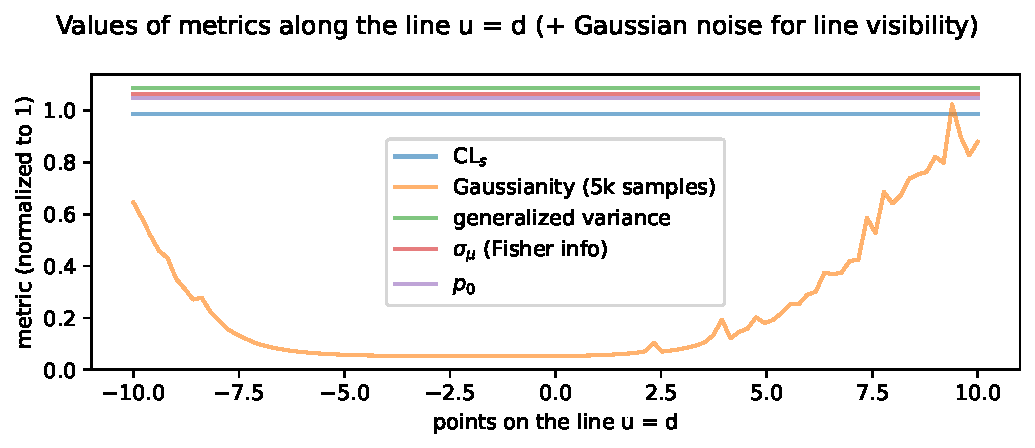
\includegraphics{./images/equal-g.pdf}

}

\caption{\label{fig-ud}A projection of the line \(u = d\) for all
metrics, which are normalized by their maximum value. A small constant
noise value is added to each metric in order to see all the lines at
once.}

\end{figure}

\hypertarget{gaussian-blobs-again}{%
\section{Gaussian blobs, again}\label{gaussian-blobs-again}}

Inspired by the studies in the previous section, I thought it would be
useful to try the study from the \texttt{neos} paper a second time, but
with some additional loss functions that we havent touched on yet
(e.g.~the discovery significance). Moreover, it may be illustrative to
track the values of all the possible loss functions for each training
strategy. In this way, we'll be able to capture some idea of the
relationships between quantities of interest -- at least within the
scope of the example itself.

We'll look at the following choices for the training objective:

\begin{itemize}
\tightlist
\item
  BCE with data augmentation (serving again as a strong baseline)
\item
  \(\mathrm{CL}_s\)
\item
  \(p_0\)
\item
  \(\sigma_{\mu}\)
\item
  \(\mathrm{CL}_s\) + \(p_0\) (inspired by the previous section)
\end{itemize}

The pipeline is exactly the same as in Section~\ref{sec-neos}, but with
slightly different hyperparameters. The only ones that differ are:

\begin{itemize}
\tightlist
\item
  5-layer neural network of size (128, 128, 128, 128, 1)\footnote{Initially,
    this was chosen to be less wide to maybe slow down the learning
    process a touch, though the extra layers mitigates that to some
    degree. It turned out that this made the training much more stable
    for some reason (less variability in the metrics), so I kept it.}
\item
  More epochs (\textasciitilde100) with the same batch size of 2000 to
  view the learning process over a longer period of time (it looks like
  some curves in Figure~\ref{fig-neos-results} would keep reducing with
  more training)
\item
  Average over nine random seeds (previously seven -- just a time
  constraint on both accounts)
\item
  Bandwidth of 0.09 for the bKDE, found through trial and error by
  making it as small as possible while still producing stable training
  runs
\end{itemize}

As an additional layer of complexity, we'll look at how the different
training strategies perform when using a lower and higher number of bins
for the neural network observable, to see if that influences the
efficacy of the methods. The bandwidth should then in theory be shrunk
in proportion to match the smaller bin widths, though

\hypertarget{bin-observable}{%
\subsection{5-bin observable}\label{bin-observable}}

\hypertarget{metrics}{%
\subsubsection*{Metrics}\label{metrics}}
\addcontentsline{toc}{subsubsection}{Metrics}

\begin{figure}

{\centering \includegraphics{./images/test_metricsfewnobins.pdf}

}

\caption{\label{fig-newneos-5bin-fixed}Plots of the different metrics
calculated on the test set for different training strategies using a
5-bin neural network observable. The results are averaged across 9
random seeds for the weight initializations. The scatter points on some
of the curves represent the model that we would select in practice if
using that training strategy (provided we decide to use the loss as the
selection metric).}

\end{figure}

We'll start by looking at the overall metrics when optimizing a 5-bin
observable. These are shown in Figure~\ref{fig-newneos-5bin-fixed},
where the circular points show the epoch where we would stop training
and select that set of models across all the random seeds (being loose
with the distiction between validation and test sets in this toy problem
setting). To recap the differences to Figure~\ref{fig-neos-results}:
we're using a slightly different neural network (deeper \& narrower),
training for longer, and tracking all the different metrics for each
training strategy.

By looking at the various metrics, we can see that training to minimze
binary cross-entropy quickly converges to its best performance, since
it's not too difficult to separate the nominal signal and background
samples from each other in data space (teal vs orange points). It's
worth pointing out that the small minima that appear early on in the
three inference-aware metrics aren't actually attained by the
``optimal'' solution that we decide on from looking at BCE alone. Even
if we don't train using those metrics, it then may still be worth
tracking them to choose the best network.

When comparing BCE to other training strategies, note the difference in
discovery \(p\)-value -- apparently we miss out on a \(p\)-value that's
better by \emph{six orders of magnitude} (a difference of
\(\approx 4.75\sigma\) for those that prefer significance) if we choose
BCE over something like \(p_0\) as an objective! It's also interesting
to note that there's a very weak correlation between the models that are
more inference-aware and their respective binary cross-entropies.

Another identifiable difference I'll highlight is that training to
minimize \(\sigma_{\mu}\) is \emph{much} better than it was in the
\texttt{neos} paper! It also follows a curve that resembles that gained
from optimizing \(\mathrm{CL}_s\) for most of the metrics, which is much
more in-line with expectations: remember that minimizing
\(\mathrm{CL}_s\) will also minimize some version of \(\sigma_{\mu}\)
too! So why were they so different in the \texttt{neos} paper? Well, the
reason I seemed to stumble upon is that the wider and more shallow
network of size (1024, 1024, 1) produces results with much higher
variance for some reason when trained to optimize \(\sigma_{\mu}\). This
is reflected in a statistic I didn't show in the initial \texttt{neos}
studies -- the networks trained with different random seeds for the
network parameters had very high variance! Why this occured for
\(\sigma_{\mu}\) in particular is unclear to me, but the results with
the narrower, deeper network used here are far more stable, which will
be seen again when we dive into some of the resulting models.

As to why the the Fisher information estimate of \(\sigma_{\mu}\)
minimizes \(\mathrm{CL}_s\) much more than \(p_0\), there are a number
of potential causes. Here, we evaluate the Fisher information using
Asimov data with \(\mu'=\gamma'=1\), i.e.~the nominal signal +
background hypothesis; earlier I said it shouldn't matter too much what
this choice is, but it could play a factor that \(\mathrm{CL}_s\) also
uses this Asimov data configuration. It could also stem from the fact
that \(q_0 \neq q_\mu\), but that's pure speculation at this point --
this should be studied further in future. The one definite takeaway is
that all these metrics care about minimizing \(\sigma_{\mu}\) in some
fashion, even if their mutual relationships are more complicated.

Commenting on other features: the new player in the game is the
discovery \(p\)-value \(p_0\), which performs pretty well in the three
inference aware metrics. It's curious to note that choosing
\(\mathrm{CL}_s\) or \(p_0\) as a training strategy limits the
performance in the other to a degree, though this is alleviated when
training using their combination \(\mathrm{CL}_s + p_0\) (as would be
expected). There is a saying though -- when one uses a metric as a
training objective, it ceases to function well as a measure of
performance, so we should take this all with a grain of salt and some
lemon zest. In some ways this saying is only partially true here, as
these metrics are calculated using a regular histogram instead of a
bKDE, so they differ in a mild conceptual way. But despite that, all of
\(\mathrm{CL}_s\), \(p_0\), and adding them together seem to perform
identically with the value of \(\sigma_{\mu}\) they end up with.

There's a couple of good performances that are worth highlighting --
optimizing with respect to \(\sigma_{\mu}\) seems to match or beat using
\(\mathrm{CL}_s\) as the training goal within its own metric for one! It
could be that it's an easier metric to minimize in practice, and so it
reaches its optimal value much faster. Though, neither \(\mathrm{CL}_s\)
nor \(\sigma_{\mu}\) seem to be super great at optimizing for \(p_0\)
(but they handily beat binary cross-entropy). Using
\(\mathrm{CL}_s + p_0\) also ends up with a slightly better \(p_0\) by a
small amount than using \(p_0\) as the objective, while not compromising
on any of the other metrics.

As a supplement to the metrics we just examined, it's interesting to see
the types of observable that the network learns for each metric. For
this, I've plotted the resulting histograms for each training strategy
that were learned by the best-performing models over each random seed.
These histograms are further augmented by plots of the value of the
neural network observable across data space, where the contours used are
exactly the same as the bin intervals; you can do a one-to-one
comparison by looking at the points enclosed in one contour, and find
the bin that corresponds to that interval, where you'll see those points
accumulated (after scale factors are applied). Many plots are ahead, and
we could talk about them for a long time, but they're mainly there to
try to give you the maximally verbose version of this study -- some
brief summative comments are provided that point out some of the
features I notice to aid your mental dissection.

Consistent shapes of learned histograms are found in most metrics, with
\(p_0\) showing the most variability. You'll notice that sometimes the
order of the bins appears to flip -- that's purely based on the nature
of the random seed, and which side shows higher significance first
during training. In many of the inference-aware metrics, we see a lot of
bins that try to balance the up and down variations of the background,
which were shown to be the best-case performance for our two-bin model
in Section~\ref{sec-which-loss-model}. Moreover, this is apparently a
more important condition for \(\mathrm{CL}_s\) and
\(\sigma_{\hat{\mu}}\) than it is for \(p_0\); the former tend to favor
an even spread of equal up and down variations across all bins, while
the latter seems to prefer isolated signal bins with no events from
background or variations thereof.

In the neural network contours, e.g.~in
Figure~\ref{fig-grid-5bin-discovery}, we can see again the effect of
\(p_0\) aggressively trying to isolate the signal within the contours,
whetheras \(\mathrm{CL}_s\) and \(\sigma_{\hat{\mu}}\) prefer contours
with balanced contributions from the up and down variations. The general
pattern though in most cases is that the contours appear to curve around
the signal for our inference aware metrics, whether as binary cross
entropy just tries to draw a good dividing line between the orange
(background) and teal (signal) blobs.

\begin{figure}

{\centering \includegraphics{./images/new-hist-models-bce-5nobin.pdf}

}

\caption{\label{fig-hists-5bin-bce}Histograms from optimizing with
respect to binary cross-entropy between signal and nominal background.}

\end{figure}

\begin{figure}

{\centering \includegraphics{./images/new-hist-models-discovery-5bin.pdf}

}

\caption{\label{fig-hists-5bin-discovery}Histograms from optimizing with
respect to the discovery \(p\)-value \(p_0\).}

\end{figure}

\begin{figure}

{\centering \includegraphics{./images/new-hist-models-CLs-5nobin.pdf}

}

\caption{\label{fig-hists-5nobin-CLs}Histograms from optimizing with
respect to the \(\mathrm{CL}_s\).}

\end{figure}

\begin{figure}

{\centering \includegraphics{./images/new-hist-models-COMB-5nobin.pdf}

}

\caption{\label{fig-hists-5bin-comb}Histograms from optimizing with
respect to a combination of discovery \(p\)-value and
\(\mathrm{CL}_s\).}

\end{figure}

\begin{figure}

{\centering \includegraphics{./images/new-hist-models-poi_uncert-5nobin.pdf}

}

\caption{\label{fig-hists-5bin-poi-uncert}Histograms from optimizing
with respect to the Fisher information estimate of
\(\sigma_{\hat{\mu}}\).}

\end{figure}

\begin{figure}

{\centering \includegraphics{./images/new-grid-models-bce-5nobin (1).pdf}

}

\caption{\label{fig-grid-5bin-bce}Contours of the neural network output
from optimizing with respect to binary cross-entropy between signal and
nominal background. The test set points are overlayed.}

\end{figure}

\begin{figure}

{\centering \includegraphics{./images/new-grid-models-discovery-5nobin (1).pdf}

}

\caption{\label{fig-grid-5bin-discovery}Contours of the neural network
output from optimizing with respect to the discovery \(p\)-value
\(p_0\). The test set points are overlayed.}

\end{figure}

\begin{figure}

{\centering \includegraphics{./images/new-grid-models-CLs-5nobin (1).pdf}

}

\caption{\label{fig-grid-5bin-CLs}Contours of the neural network output
from optimizing with respect to the \(\mathrm{CL}_s\). The test set
points are overlayed.}

\end{figure}

\begin{figure}

{\centering \includegraphics{./images/new-grid-models-COMB-5nobin (1).pdf}

}

\caption{\label{fig-grid-5bin-comb}Contours of the neural network output
from optimizing with respect to a combination of discovery \(p\)-value
and \(\mathrm{CL}_s\). The test set points are overlayed.}

\end{figure}

\begin{figure}

{\centering \includegraphics{./images/new-grid-models-poi_uncert-5nobin (1).pdf}

}

\caption{\label{fig-grid-5bin-poi-uncert}Contours of the neural network
output from optimizing with respect to the Fisher information estimate
of \(\sigma_{\hat{\mu}}\). The test set points are overlayed.}

\end{figure}

\hypertarget{bin-observable-1}{%
\subsection{20-bin observable}\label{bin-observable-1}}

Now we can see what happens when we provide a lot more bins to play
with!

\hypertarget{metrics-1}{%
\subsubsection*{Metrics}\label{metrics-1}}
\addcontentsline{toc}{subsubsection}{Metrics}

\begin{figure}

{\centering \includegraphics{./images/test_metricsmanynobins.pdf}

}

\caption{\label{fig-newneos-20bin-fixed}Plots of the different metrics
calculated on the test set for different training strategies using a
20-bin neural network observable. The results are averaged across 9
random seeds for the weight initializations. The scatter points on some
of the curves represent the model that we would select in practice if
using that training strategy (provided we decide to use the loss as the
selection metric).}

\end{figure}

The story doesn't change too much with more bins, with all the training
strategies maintaining their mutual relationships as discussed earlier.
The only marked difference is that \(p_0 + \mathrm{CL}_s\) outperforms
\(p_0\) alone much more clearly here, which is pretty interesting to
think about.

I'll also show the histograms and neural network contours in data space
-- there are some pretty funky ones for the high-bin case. You'll see
that the types of histogram model learned by the neural network
fluctuate much more with this additional granularity provided by the new
bins, especially for the hypothesis test-based metrics (seed 2 and 3 are
particularly strange for \(p_0\)).

For the contours themselves, there are many things to see here, but I'll
just point out one of my favourites: for seed 3 in
Figure~\ref{fig-hists-20nobin-CLs} and
Figure~\ref{fig-hists-20bin-discovery}, we see the network struggling to
untie the systematic variations from the signal bins. However, for the
same seed in Figure~\ref{fig-hists-20bin-comb}, where we're training on
a combination of those metrics, the network seems to manage! No idea why
this behaviour is there, and indeed it is just one seed. But I thought
that was pretty cool.

\begin{figure}

{\centering \includegraphics{./images/new-hist-models-bce-20nobin.pdf}

}

\caption{\label{fig-hists-20bin-bce}Histograms from optimizing with
respect to binary cross-entropy between signal and nominal background.}

\end{figure}

\begin{figure}

{\centering \includegraphics{./images/new-hist-models-discovery-20nobin.pdf}

}

\caption{\label{fig-hists-20bin-discovery}Histograms from optimizing
with respect to the discovery \(p\)-value \(p_0\).}

\end{figure}

\begin{figure}

{\centering \includegraphics{./images/new-hist-models-CLs-20bin.pdf}

}

\caption{\label{fig-hists-20nobin-CLs}Histograms from optimizing with
respect to the \(\mathrm{CL}_s\).}

\end{figure}

\begin{figure}

{\centering \includegraphics{./images/new-hist-models-COMB-20nobin.pdf}

}

\caption{\label{fig-hists-20bin-comb}Histograms from optimizing with
respect to a combination of discovery \(p\)-value and
\(\mathrm{CL}_s\).}

\end{figure}

\begin{figure}

{\centering \includegraphics{./images/new-hist-models-poi_uncert-20nobin.pdf}

}

\caption{\label{fig-hists-20bin-poi-uncert}Histograms from optimizing
with respect to the Fisher information estimate of
\(\sigma_{\hat{\mu}}\).}

\end{figure}

\begin{figure}

{\centering \includegraphics{./images/new-grid-models-bce-20nobin (1).pdf}

}

\caption{\label{fig-grid-20bin-bce}Contours of the neural network output
from optimizing with respect to binary cross-entropy between signal and
nominal background. The test set points are overlayed.}

\end{figure}

\begin{figure}

{\centering \includegraphics{./images/new-grid-models-discovery-20nobin (1).pdf}

}

\caption{\label{fig-grid-20bin-discovery}Contours of the neural network
output from optimizing with respect to the discovery \(p\)-value
\(p_0\). The test set points are overlayed.}

\end{figure}

\begin{figure}

{\centering \includegraphics{./images/new-grid-models-CLs-20nobin (1).pdf}

}

\caption{\label{fig-grid-20bin-CLs}Contours of the neural network output
from optimizing with respect to the \(\mathrm{CL}_s\). The test set
points are overlayed.}

\end{figure}

\begin{figure}

{\centering \includegraphics{./images/new-grid-models-COMB-20nobin (1).pdf}

}

\caption{\label{fig-grid-20bin-comb}Contours of the neural network
output from optimizing with respect to a combination of discovery
\(p\)-value and \(\mathrm{CL}_s\). The test set points are overlayed.}

\end{figure}

\begin{figure}

{\centering \includegraphics{./images/new-grid-models-poi_uncert-20nobin (1).pdf}

}

\caption{\label{fig-grid-20bin-poi-uncert}Contours of the neural network
output from optimizing with respect to the Fisher information estimate
of \(\sigma_{\hat{\mu}}\). The test set points are overlayed.}

\end{figure}

\hypertarget{optimizing-binning-and-neural-network-simultaneously}{%
\subsection{Optimizing binning and neural network
simultaneously}\label{optimizing-binning-and-neural-network-simultaneously}}

One thing I also thought to try is, for a fixed number of bins,
exploring what happens when the bin edges are made to be \emph{part of
the optimization itself}. Our free parameters are then
\(\varphi = \left\{\varphi_{\mathrm{nn}}, \text{bin edges}\right\}\). To
prevent the bin edges from being non-ascending, a
\texttt{jax.numpy.where} statement was used to replace values that were
larger than their neighboring edge with something just below it instead.
As opposed to bin edges, we could have equivalently let the bin widths
vary instead, and decide the last width as
\(1-\sum_{i=0}^{\text{number of bins - 1}} \text{bin widths}_i\). In
practice, this was found to be less stable when tried (often the sum of
widths would exceed 1, and the last width becomes negative in that
case). The endpoints \([0,1]\) were taken as fixed to ensure there isn't
optimization that accounts for the bKDE spilling out outside that range.
In hindsight, though, I think things would be fine without this
restriction, especially since the best network is selected based on the
the version of the loss with no approximations (i.e.~a pipeline that
uses a regular histogram with the optimized binning).

Results from this experiment are fairly similar to the fixed-bin case,
and are shown in Appendix~\ref{sec-bins-app}. The most notable finding
is that \(\sigma_{\hat{\mu}}\) seemed to be the metric that made use of
adapting the binning the most, but didn't necessarily translate this to
a big performance gain.

\hypertarget{whats-next}{%
\section{What's next?}\label{whats-next}}

The first question that arises when reading this work for most -- which
mirrors accurately the same question I get when giving talks about this
-- is \emph{how does it scale to optimize with a \(p\)-value?} Great
question; I wish I knew. I've not personally managed to apply this to a
real use-case where this method could thrive (e.g.~a physics analysis
where systematic uncertainties serve as a bottleneck for performance).
But if we were to do so, scaling will come with some challenges: the
first being that the accuracy of the model construction per iteration is
dependent on the batch size being large enough to faithfully represent
the analysis. In practice, this was overcome by applying scale factors
to the batches that normalized their event counts to something expected
by the whole sample (in our toy case, we made the arbitrary choice of a
1/5 ratio between signal and background, with a normalization to around
\textasciitilde10 events or so). Moreover, the unavoidable truth already
mentioned in Section~\ref{sec-neos-issues} is that the cost of the
forward pass + backward pass =
\textasciitilde{}\(\mathcal{O}(2\times \text{analysis cost})\), which
may scale in complicated ways depending on the complexity of the model
at hand. One would probably need to prune any workspace to only include
systematic uncertainties that have been studied to impact the analysis
result significantly.

A whole world of things could be targets for being made differentiable.
As a simple extension to what's already been shown here, one could
imagine making upper limits differentiable in the same way as the
profile likelihood; there's no conceptual restriction, but since there's
an optimization procedure to determine the upper limit (find the value
of the parameter that gives a certain \(p\)-value), we can reuse the
idea of implicit gradients that exist for functions with fixed points.
There's also a nice
\href{http://github.com/gradhep/relaxed/list_of_operations.md}{set of
operations that could benefit from being differentiable} curated by Kyle
Cranmer, including things like sorting, statistical methods, and peer
review (perhaps more relevant after AI take over the world -- we can
optimize their weights to help us get accepted at major
conferences)\footnote{Thinking about it though, AI having a workshop
  about the workings of AI would be more like biology/philosophy.
  Perhaps this whole thesis is then unethical through this lens,
  exploiting and manipulating machines for our own curiosity. The
  complementary idea of inverting this exploitation is a rather
  dystopian one.}. It's possible that I've gotten around to implementing
some of these in
\href{http://github.com/gradhep/relaxed}{\texttt{relaxed}} (Simpson
2022a) by the time you read this, which is a differentiable toolbox of
sorts that implements all of the advances that you've seen in this
chapter.

While we're on the topic, one particularly cool thing about
\texttt{relaxed} is that it mimics the APIs of commonly used software
tools in HEP. As an example, hypothesis tests are usually done with
\href{http://github.com/scikit-hep/pyhf}{\texttt{pyhf}} using the
one-liner

\begin{Shaded}
\begin{Highlighting}[]
\NormalTok{pyhf.infer.hypotest(}
\NormalTok{    mu\_0,  }\CommentTok{\# null hypothesis for mu}
\NormalTok{    data,}
\NormalTok{    model,}
\NormalTok{    test\_stat,  }\CommentTok{\# = q\_mu or q\_0}
\NormalTok{)}
\end{Highlighting}
\end{Shaded}

And indeed, the same call works for \texttt{relaxed}, with the bonus
being you can differentiate the result:

\begin{Shaded}
\begin{Highlighting}[]
\NormalTok{relaxed.infer.hypotest(}
\NormalTok{    mu\_0,  }\CommentTok{\# null hypothesis for mu}
\NormalTok{    data,}
\NormalTok{    model,}
\NormalTok{    test\_stat,  }\CommentTok{\# = q\_mu or q\_0}
\NormalTok{    lr }\OperatorTok{=} \FloatTok{1e{-}3}  \CommentTok{\# learning rate for fits (done with grad descent)}
\NormalTok{)}
\end{Highlighting}
\end{Shaded}

To see more of what this looks like in practice, I encourage you to
check out the \href{http://github.com/gradhep/relaxed}{repository
(e.g.~the tests)}, a
\href{http://github.com/phinate/differentiable-analysis-examples}{set of
examples that I wrote} (Simpson 2022b), and my
\href{https://youtu.be/cOv7W-moO6k}{PyHEP 2022 video tutorial}.

Beyond quantities that stem from statistical inference, differentiable
simulation is another promising area that could allow
simulator-in-the-loop optimization. An example could be tuning your
simulator parameters to model data by gradient descent, or perhaps
having a pipeline with a loss function that simulates physics on-the-fly
based on learned parameters. Moreover, there has been a very interesting
recent line of work that looks at making key physics processes
differentiable, such as the calculation of matrix elements for
scattering amplitudes (Heinrich and Kagan 2022) and parton showering
(Nachman and Prestel 2022). This is certainly an area to keep an eye on
over the coming years.

\hypertarget{credits}{%
\section{Credits}\label{credits}}

Many thanks go to Lukas Heinrich for the inspiration, debugging help,
and original proposal, and also to Tomasso Dorigo/Pablo de Castro for
their initial assistance and work on INFERNO (Castro and Dorigo 2019),
which lay lots of the groundwork for this topic. Thanks also to the
other \texttt{pyhf} authors Matthew Feickert and Giordon Stark, and to
Alex Held for his great notebook on differentiable cuts and other
advice.

\hypertarget{sec-flow-interp}{%
\chapter{Signal Model Interpolation using Normalizing
Flows}\label{sec-flow-interp}}

One of the primary goals of data analysis in collider physics is to test
the viability of proposed models for new physics, which attempt to
address the shortcomings of the well-tested Standard Model. We'll call
these models the \textbf{signal}. Since we don't have access to real
data from these hypothesized phenomena, we use high-quality simulations
of the underlying physics to generate samples that mimic data collected
from major experiments, e.g.~the Large Hadron Collider. This then lets
us identify the most prominent signature that physics process leaves in
the data, such as the shape of the invariant mass of some particular
final state. We can compare that signature with data generated to mimic
the same final state, but with only standard model processes (which we
term \textbf{background}), and use this comparison as a mechanism to
produce an analysis that \emph{could} discover the signal if it were
present. This can then be applied to real data.

How many models are there to test? In general, there's no upper limit --
arXiv grows thicker every day with more theory model submissions. But
what about within a certain class of model with \emph{similar free
parameters}? This scope-narrowing makes our lives much easier, as we're
only now limited by the parameters of the model, e.g.~the mass of a new
particle. One could then imagine testing each possible value for this
new mass\ldots{} until we realize that there's only so many times we can
do this. Recall that simulating data is in general expensive, and we'd
rather avoid it where we can. Moreover, if we have a multi-dimensional
parameter space to explore, covering that in an efficient way will be
prohibitively expensive to simulate. How do we get around this?

Well, if we're interested in some signature from the model in a
particular set of variables, we could generate that data for a set of
parameters, then find some way to interpolate between them.
Specifically, this can be viewed as trying to estimate the probability
density (or \emph{shape}) of a variable of interest, where we want to
\emph{condition} on the physics parameters involved in the generation of
that shape. This is the approach taken here.

It's worth noting that physics analyses typically don't interpolate on
the level of the statistical model, and instead just interpolate the
result of the search itself, e.g.~in the space of \(p\)-values or on
limits for the signal strength \(\mu\) across a grid of e.g.~different
signal masses. This is often quoted without error (a different issue),
and does not take into account the fact that we'd expect to be less
sensitive to new physics in the regions that we don't have high-quality
simulations for. However, if one can interpolate the signal model in
some way \emph{before} calculating the final result, then incorporate a
predictive uncertainty from that interpolation into the statistical
treatment of the data, we should hopefully be able to have a more
grounded representation of our sensitivity between simulated signal
model points.

\hypertarget{problem-statement}{%
\section{Problem statement}\label{problem-statement}}

Say a simulated signal process outputs a set \(\mathbf{x}\) of per-event
physics quantities (or \textbf{observables}), where each quantity is
typically a real number (e.g.~kinematics). We're interested in making a
statistical model of this process, and so take interest in the
distribution over \(\mathbf{x}\), which we'll denote
\(p_s(\mathbf{x} | \theta)\), with \(\theta\) representing the free
parameters of the physical model (and \(s\) standing for signal). We can
partition \(\theta\) as \(\theta = [\phi, \nu]\), where \(\phi\)
effectively parametrizes the hypothesis of the new physics model
(e.g.~through the mass of a new particle), and \(\nu\) represents
parameters that are needed to specify the physics conditions, but are
not of interest (e.g.~a jet energy scale). We focus on conditioning with
respect to \(\phi\) here, and leave treatment of \(\nu\) as part of the
statistical modelling process (see Section~\ref{sec-hifa-nps} for more
on this).

We don't have a way to calculate this density due to our inability to
access the implicit distribution defined by the simulator, but we do
have access to the samples themselves (at some finite number of values
of \(\theta\)). This means we can empirically estimate the distribution
in some way, provided we have the right tools to do so. If successful,
we're free to directly use this empirical estimation of
\(p_s(\mathbf{x} | \theta)\), but in practice, we're often faced with an
additional modelling constraint: many analyses in collider physics
operate using \emph{histograms} of observables, and construct a
statistical model based on that. As such, it would be desirable if we
could find a density estimator that:

\begin{itemize}
\tightlist
\item
  allows for the \emph{conditioning} of side variables (here, this would
  be conditioning on \(\phi\))
\item
  has a tractable likelihood (e.g.~for direct use in ``unbinned''
  analysis)
\item
  can model discrete densities like a histogram

  \begin{itemize}
  \tightlist
  \item
    or, optionally, allow the generation of samples that can be
    histogrammed later
  \end{itemize}
\item
  (optionally) comes with a notion of uncertainty
\end{itemize}

This brings us to normalizing flows!

\hypertarget{normalizing-flows-recap}{%
\section{Normalizing flows (recap)}\label{normalizing-flows-recap}}

A much more extensive motivation for normalizing flows can be found in
Section~\ref{sec-flows}, but we'll recap the main points here.

Normalizing flows are a class of density estimation technique, which
attempts to transform a designated \emph{base} density into a *target
density with the aid of neural networks. This admits the ability to
sample from a flow, since you can just transform the samples from the
base density, which is usually of simple form (e.g.~normal
distribution). Moreover, flows have a tractable likelihood, which can be
evaluated by transforming the samples using the learned transform,
putting that into the base density, and multiplying by the relevant
Jacobian, effectively bending the space into the desired shape to mimic
the target density.

To train a flow, we simply fit samples from the base distribution to the
training samples such that the negative log-likelihood of the flow model
is minimized. This is done across batches of different training data,
just as in standard machine learning optimization.

All of the properties of a flow satisfy most of the bullets above for
our criteria, but we're still missing two parts: conditioning and
uncertainty. These are addressed in the following sections.

\hypertarget{implementing-conditional-density-estimation}{%
\subsection{Implementing conditional density
estimation}\label{implementing-conditional-density-estimation}}

A few different types of models allow for conditional density
estimation, e.g.~RealNVPs (Dinh, Sohl-Dickstein, and Bengio 2016), MADE
(Germain et al. 2015), and masked autoregressive flows (MAFs)
(Papamakarios, Pavlakou, and Murray 2017) -- we focus on the latter as
the choice for this task. Details on the precise implementation of a MAF
can be found in Section~\ref{sec-maf}.

\hypertarget{estimating-predictive-uncertainty}{%
\subsection{Estimating predictive
uncertainty}\label{estimating-predictive-uncertainty}}

If we're using the likelihood (or a histogram of the samples) to make a
prediction using the flow, we don't have a natural way to produce a
corresponding uncertainty on that prediction. One way to get around this
fact is to take inspiration from the notion of \textbf{model ensembles}
(see a review in (Ganaie et al. 2021)), which combine multiple
predictive models into one by averaging their predictions at a given
point, then providing an uncertainty through the sample standard
deviation across those predictions. The intuition behind this is that
one would expect models to have the most mutual variance in the region
where there is no training data, as that lies outside of the context
that the models learned. There's no particular way in which one needs to
form the different elements of an ensemble for it to have some
reasonable utility, but one common strategy in the land of neural
networks is to train a few models with different weight initializations,
and use those as the models to make up the ensemble. This approach is
what we do here: both with the likelihood functions, and with the
histogram yields produced from samples of those flows.

\hypertarget{example-1-following-the-mean}{%
\section{Example 1: Following the
mean}\label{example-1-following-the-mean}}

To test out the MAF as a conditional density estimator, it suffices to
model some family of distributions parametrized by some context
\(\phi\), just as we set out in the problem statement. One thing I
thought of when considering this is a 2-D normal distribution, where the
mean represents the context. This should be a simple starting problem,
and is a similar use case to that which I encountered in a physics
context, where the signature left in the invariant mass spectrum
clustered around the value of the rest mass of the particles that
produced it. We'll add more complexity to this later.

We'll start by sampling a range of normal distributions with different
means and unit covariance. The means here are the \emph{context} -- the
thing we'll condition on during training and inference. Training data
will then consist of pairs of samples from these distributions, and the
mean of the distribution that generated the samples. We'll also split
the different distributions up into context points that are used for
training, and unseen points that are used for validation and testing (in
practice, these should be two distinct tasks, but we'll combine them for
these examples to portray the proof-of-concept in a best-case way).
Points in the test set are not seen during training; we use them purely
to assess performance (and select a good model) when interpolating to a
context not seen before.

As a small note here, we also hold out a small number of examples (20\%
per point) from the training set to use as additional validation in
conjunction with the unseen context points. These together are referred
to as the ``valid'' set in the loss curve plots, and are used only for
model selection purposes, including making sure we're not totally
biasing our selection to the small number of unseen context points (we
want to make sure performance on the whole grid is maintained). This is
a hyperparameter that could be played with, or discarded altogether.
More discussion on this can be found later on.

The distributions chosen are shown in Figure~\ref{fig-normalgrid}, where
49 different means have been evenly selected across a grid of points,
indicated by crosses colored by the set they belong to. Note that the
test set points are chosen such that they're all \emph{inside} the grid
-- this is because we're seeking to interpolate our results within the
region we have data as opposed to extrapolate outside of it.

\begin{figure}

{\centering \includegraphics{./images/flows/simple/simple_data_dists.pdf}

}

\caption{\label{fig-normalgrid}A grid of 49 different normal
distributions, each with a mean corresponding to a cross on the image,
and with unit covariance. The contour representing 0 is omitted for
visualization purposes.}

\end{figure}

10,000 points are then drawn from each distribution, and 3 MAFs are
trained on the same training data, but with different weight
initializations. The hyperparameters for training those MAFs are as
follows:

\begin{itemize}
\tightlist
\item
  Batch size of 4000 points
\item
  10 layers of linear, autoregressive transforms

  \begin{itemize}
  \tightlist
  \item
    Each transform's neural network has one hidden layer of 6 neurons
  \end{itemize}
\item
  Adam optimizer with a learning rate of 1e-3
\item
  3000 iterations total (common reasonable plateau point for all
  examples)
\end{itemize}

During training, the inputs and context are each scaled to standard
normal distributions through fitting a \texttt{StandardScaler} from
Scikit-Learn (Pedregosa et al. 2011) to the train data. Any samples
produced from the flow are then transformed back using this same scaler.
Training was done using the \texttt{nflows} software package (Durkan et
al. 2020), which builds on PyTorch (Paszke et al. 2019).

It's worth noting that since we trained three MAFs, when I refer to the
``flow'' in later sections, I'm referring to the ensemble of all three
models, where their predictions (either likelihoods or histograms) are
averaged together, and their predictive uncertainty is the corresponding
standard deviations.

We can examine the results of the training through different types of
visualizations, as we'll see below:

\hypertarget{loss-curves}{%
\subsection{Loss curves}\label{loss-curves}}

See Figure~\ref{fig-simple-loss} for a comparison of the negative
log-likelihood loss for train and test sets. This is for just one of the
three flows, and shows the similarity of the train and test losses due
to the fact that the train and test data are so similar (there's not
much domain shift needed, just learning the position of the mean).

\begin{figure}

{\centering \includegraphics{./images/flows/simple/simple_example_loss.pdf}

}

\caption{\label{fig-simple-loss}Example loss curves from a single flow
trained on the ``following the mean'' scenario. The model weights are
extracted from the best test loss.}

\end{figure}

\hypertarget{distribution-similarity}{%
\subsection{Distribution similarity}\label{distribution-similarity}}

It's illustrative to plot the likelihoods learned by the flow for each
of the context points, including the ones for which we didn't see during
training. We could, in theory, supply any value of the context for this
evaluation, but it's much more useful to do it in the region that we
have test data so we can compare the result.

We can find this plot in Figure~\ref{fig-simple-lhoods}, where the plot
from Figure~\ref{fig-normalgrid} is shown as a comparison metric
side-by-side. We can immediately see that the likelihood shapes are
about what we'd expect, but we note the contours are coloured in log
scale for the flow, which is done so to enhance visibility of the shape
close to the mean, since the contours increase more rapidly in value
around the center of the distribution. Additionally, the values of the
normalization are much higher for the flow, which can be attributed to
the fact that the training data is very concentrated around the mean,
and so a distribution with all it's density there will quickly give a
good solution, as opposed to distributing that over a larger range in a
more diffuse way. This could likely just be due to the training data
being capped at 10k points.

\begin{figure}

{\centering \includegraphics{./images/flows/simple/simpleflowvsdata.pdf}

}

\caption{\label{fig-simple-lhoods}Left: the same grid of 49 different
normal distributions from Figure~\ref{fig-normalgrid}. Right: the
learned likelihood from the flow evaluated with context equal to the
values of the means from the grid.}

\end{figure}

This is a nice visual check, but it's probably more useful to quantify
this similarity in some way.

\hypertarget{histogram-similarity}{%
\subsection{Histogram similarity}\label{histogram-similarity}}

Since we're interested in possibly using the result as a histogram, we
can directly compare histograms of samples from the flow with histograms
of the original data. Plots of the raw data versus flow differences can
be found in Figure~\ref{fig-simple-hists-train} for training points, and
Figure~\ref{fig-simple-hists-test} for test points. The plots are made
using a histogram of the whole dataset for each context point (10k data
points in total per histogram) versus a histogram of 100k samples
conditioned on the same context points from the flow to get the overall
shape, which is then re-normalized back to 10k overall counts. The x-y
axes are omitted for a cleaner plot, but the histogram range is around
+/- 2.5 in each direction about the mean (imagine a square around one of
the distributions in Figure~\ref{fig-normalgrid}).

\begin{figure}

{\centering \includegraphics{./images/flows/simple/simplehistdifftrain-reallyunscaled.pdf}

}

\caption{\label{fig-simple-hists-train}Differences between flow and data
histograms across training context points, where each histogram is of
10k data points. 10 points are chosen randomly. The red cross marks the position of the mean of the
true distribution.}

\end{figure}

\begin{figure}

{\centering \includegraphics{./images/flows/simple/simplehistdifftest-errors.pdf}

}

\caption{\label{fig-simple-hists-test}Differences between flow and data
histograms across unseen, test set context points, where each histogram
is of 10k data points. The red cross marks the position of the mean of
the true distribution.}

\end{figure}

The main thing we can get from this visualization is the imprint that
subtracting the flow histogram from the data leaves. We can see this
more prominently in Figure~\ref{fig-simple-hists-test}, where there are
some biases left from the flow network getting the area around the mean
slightly off. Green represents where the data counts are larger, and
brown represents where the flow predicts larger counts. The scale of the
colorbar in each case is worth noting -- for a histogram of size 10k,
these are relatively tame differences, but differences nonetheless
(relative bin-wise differences would also be nice to view, but are
inflated somewhat by small bin counts away from the mean).

\hypertarget{pulls}{%
\subsection{Pulls}\label{pulls}}

These plots are only half the story; we'd much rather see how the flow
\emph{uncertainties} affect these results. Instead of doing this
bin-by-bin where small localized uncertainties make for difficult
visualization, we plot the \emph{pulls} aggregated over all training and
test points separately. The pull here for one bin is defined as

\[
\text{pull } = \frac{\text{flow prediction }-\text{ data prediction}}{\sigma_{\text{flow}}}~,
\]

where the uncertainty \(\sigma_{\text{flow}}\) comes from the standard
deviation of the counts from the three histograms in that bin, which
were produced by sampling each flow in turn. Without making any strong
theoretical claim, the reasoning to plot this quantity is to loosely
follow the intuition behind the central limit theorem, where we assume
that the bin counts will tend to a normal distribution in the limit of
many repeated experiments. If the flow is a good predictor of the mean
of that normal distribution, we'd observe the data being distributed as
approximately \(\mathrm{Normal}(\text{flow}, \sigma_{\mathrm{flow}})\).
This ballpark statement is somewhat realized in
Figure~\ref{fig-simple-pulls}, where we plot histograms of the pull
aggregated across all training contexts (left plot) and testing contexts
(right plot).

The results are fairly unbiased in either case, with a spread of pulls
being fitted a little wider than a standard normal. Beyond this, it's
clear that if the error in the denominator is of comparable to the
difference between data and flow, we're fairly happy that we know where
we're wrong to some degree. Using this ensemble uncertainty is then a
reasonable way to predict the failure modes of the flow for this simple
example.

\begin{figure}

{\centering \includegraphics{./images/flows/simple/simpleflowpulls.pdf}

}

\caption{\label{fig-simple-pulls}Plot of the pull for training contexts
(left plot) and testing contexts (right plot). A fitted normal
distribution is also shown for illustrative purposes.}

\end{figure}

\hypertarget{example-2-gaussian-firework}{%
\section{Example 2: Gaussian
firework}\label{example-2-gaussian-firework}}

We now add a degree of complexity. Keeping with the theme of normal
distributions, we'll let the mean influence the covariance matrix such
that the distribution will rotate based on its position relative to the
origin. More formally, for \(\mu = [\mu_x, \mu_y]\), this
parametrization \(\mathrm{Normal}(\mu, \Sigma)\) can be constructed by
the following steps:

\[
\theta = \arctan (\mu_y / \mu_x);~~~r=\sqrt{\mu_x^2 + \mu_y^2}
\] \begin{equation}\protect\hypertarget{eq-complex-cov}{}{
\Rightarrow \Sigma = MM^T \text{,     where } M = \left[\begin{array}{cc}
\cos \theta & \sin \theta \\
-\sin \theta & \cos \theta
\end{array}\right] \left[\begin{array}{cc}
1/r &0 \\
0 & 1
\end{array}\right]~.
}\label{eq-complex-cov}\end{equation}

This rather weird formula, found using inspiration from a blog post on a
geometric interpretation of the covariance in a Gaussian (Spruyt 2014),
applies a rotation and a scaling in proportion to the mean. By
generating the same grid of points as in Figure~\ref{fig-normalgrid}, we
end up with the result in Figure~\ref{fig-complex-normalgrid}. I've
affectionately termed it a Gaussian firework, since it makes a wonderful
explosive pattern when plotted symmetrically about the origin, which I
additionally show some examples of in Figure~\ref{fig-firework}.

\begin{figure}

{\centering \includegraphics{./images/flows/complex/non-simple_data_dists.pdf}

}

\caption{\label{fig-complex-normalgrid}A grid of 49 different normal
distributions, each with a mean corresponding to a cross on the image,
and with covariance as defined by Equation~\ref{eq-complex-cov}. The
contour representing 0 is omitted for visualization purposes.}

\end{figure}

\begin{figure}

\begin{minipage}[t]{0.5\linewidth}

{\centering 

\raisebox{-\height}{

\includegraphics{./images/flows/complex/cont.png}

}

\caption*{Some distributions plotted symmetrically about the \\origin.}

}

\end{minipage}%
%
\begin{minipage}[t]{0.5\linewidth}

{\centering 

\raisebox{-\height}{

\includegraphics{./images/flows/complex/disc.png}

}

\caption*{Histogram of many samples drawn from a grid of distributions
about the origin.}

}

\end{minipage}%

\caption{\label{fig-firework}A couple of fun plots to show the naming
convention of ``Gaussian firework''.}

\end{figure}

Modelling this firework is more challenging for a couple reasons. The
first is that we have some kind of symmetry of rotation that the flow
needs to pick up on, using only information from the mean. The second is
that the distributions are very tight about their means -- a slight
mis-guess will show a considerable error when making the same
visualizations as in the simple example.

The hyperparameters for the training are the same as the previous
example, including the points in the train/test sets, so we jump
straight to the results.

\hypertarget{loss-curves-1}{%
\subsection{Loss curves}\label{loss-curves-1}}

See Figure~\ref{fig-complex-loss} for a comparison of the negative
log-likelihood loss for train and test sets. Again, this is just one of
the three flows for illustrative purposes. We notice that the training
stops much earlier, which is due to the fact that the difference between
train and test sets is much more significant here, with it being easier
to overfit to the training samples alone.

\begin{figure}

{\centering \includegraphics{./images/flows/complex/non-simple_example_loss.pdf}

}

\caption{\label{fig-complex-loss}Example loss curves from a single flow
trained on the Gaussian firework scenario. The model weights are
extracted from the best test loss.}

\end{figure}

\hypertarget{distribution-similarity-1}{%
\subsection{Distribution similarity}\label{distribution-similarity-1}}

We can see the plots of the learned likelihoods from the flow ensemble
in Figure~\ref{fig-complex-lhoods}. The topic of the scale difference is
exacerbated further, which I'd guess is due to the concentrated nature
of the distribution, allowing for the clustering of all the density in
one place to quickly achieve a good loss for the training data.

We note the fairly good modelling of the way the distribution shape
varies across the training points in particular. The shape of the
distribution far from the mean at the unseen test set points (red
crosses) is a little less well-modelled, with the mean being slightly
off-center sometimes, and the contours not being as even.

\begin{figure}

{\centering \includegraphics{./images/flows/complex/non-simpleflowvsdata.pdf}

}

\caption{\label{fig-complex-lhoods}Left: the same grid of 49 different
normal distributions from Figure~\ref{fig-complex-normalgrid}. Right:
the learned likelihood from the flow evaluated with context equal to the
values of the means from the grid.}

\end{figure}

\hypertarget{histogram-similarity-1}{%
\subsection{Histogram similarity}\label{histogram-similarity-1}}

Coming again to histograms, we do the same plots as for the first
example, beginning with the raw differences in
Figure~\ref{fig-complex-hists-train} and
Figure~\ref{fig-complex-hists-test}. The scale of the errors in the
training set are equivalent to those in the simple example, but we see
that the test errors have some vast differences by comparison. Since the
distributions are so concentrated, you can effectively see the flow
distribution in brown, and the data distribution in green for the test
context points. This example is particularly unforgiving for the biases
introduced as a result of the flow not having seen these points, since a
slight mismodelling introduces a large error. Additionally, from a shape
perspective, the centers are roughly coincident, but the rotation
inferred from the context is a little different in most cases.

\begin{figure}

{\centering \includegraphics{./images/flows/complex/non-simplehistdifftrain-reallyunscaled.pdf}

}

\caption{\label{fig-complex-hists-train}Differences between flow and
data histograms across training context points for the Gaussian firework
example, where each histogram is of 10k data points. 10 points are chosen at random. The red cross marks
the position of the mean of the true distribution.}

\end{figure}

\begin{figure}

{\centering \includegraphics{./images/flows/complex/non-simplehistdifftest-errors.pdf}

}

\caption{\label{fig-complex-hists-test}Differences between flow and data
histograms across unseen, test set context points for the Gaussian
firework example, where each histogram is of 10k data points. The red
cross marks the position of the mean of the true distribution.}

\end{figure}

\hypertarget{pulls-1}{%
\subsection{Pulls}\label{pulls-1}}

Unlike in the simple example, the magnitude of the flow ensemble
uncertainty is not great enough to save us in every case when we make
the pull plots, which are shown in Figure~\ref{fig-complex-pulls}. We
see that the flow applied to the training distribution is reasonably
unbiased in its prediction of the histogram counts, but the test set is
far less forgiving -- we have some points that are extremely far from 0,
due to the flow difference being large and the uncertainty being
comparably small.

\begin{figure}

{\centering \includegraphics{./images/flows/complex/non-simpleflowpulls.pdf}

}

\caption{\label{fig-complex-pulls}Plot of the pull for training contexts
(left plot) and testing contexts (right plot) for the Gaussian firework
example. A fitted normal distribution is also shown for illustrative
purposes.}

\end{figure}

\hypertarget{sec-flow-discussion}{%
\section{Discussion}\label{sec-flow-discussion}}

By and large, this method performed fairly well on the two toy examples
it was tested on. It's clear that there is some very deliberate
contextual inference, which is found from training in a way that
conditions on the parameters that generated the samples, and generates a
good proof of context for the viability of this method. This being said,
there are definite shortcomings in the test set of the second example,
which I'll address with my thoughts below, including how it's inherently
linked to some of the training methodology decisions, and why I'm not
overwhelmingly pessimistic about it.

We can point at many things that could explain the interpolation failure
modes in the second example: flow architectures that are too inflexible
to model the very concentrated shapes, the limitation of training data
points provided (both in number of data points and context grid
density), not training with the best hyperparameters (minimal tuning was
done), or perhaps the flow ensemble was too small.

\hypertarget{whats-the-true-test-set}{%
\subsection{What's the true ``test
set''?}\label{whats-the-true-test-set}}

Another reason for interpolation failures is that removing the test set
points will fundamentally bias the model away from learning to
generalize to the points we removed, when we technically had that
information to learn from in the first place. This creates a paradox
with assuming a train and test split -- in what way should we do this?
One could think of an example involving vital medical data, where it's
essential to learn from the points provided instead of discounting large
numbers of examples for validation.

One way to do this is to just do the train/test split in the \emph{data}
instead of in the \emph{context}. That would be akin to more standard
practice in traditional machine learning, for instance, but neglects
keeping a good measure of the interpolation performance. As mentioned
previously, there was a notion of a ``valid'' set that was played with
during the examples that does this to some extent already by holding out
a small fraction of data from training context points. However, if we
did this for \emph{all} context points, we'd have to blindly trust the
flow uncertainty to account for the predictive uncertainty to new
points. One could perhaps do some k-fold or leave-one-out cross
validation, where the model's generalization ability could be
conservatively quantified by training multiple flows on data with one
context point removed, repeating this across all points in the
interpolation regime, and quote the ensemble uncertainty or the
predicted vs actual error for each of these cases as a better idea of
the predictive uncertainty. A caveat to this is that these models are
all different to the one that actually would be used in practice, and
there would have to also be some kind of secondary
interpolation/extrapolation mechanism to produce this cross-validation
uncertainty in a continuous way across the context space. These ideas
were not tried due to time constraints, but could be the subject of
further work.

In the next section, we'll re-use this method, but we'll also compare it
to statistical uncertainties in the histograms themselves, and see if we
do better than just the predictive uncertainty on the flow (not here
purely due to time).

\hypertarget{sec-anal}{%
\chapter{\texorpdfstring{Search for a heavy scalar particle \(X\)
decaying to a scalar \(S\) and a Higgs boson, with final state
\(b\bar{b}\gamma\gamma\) in the ATLAS
detector}{Search for a heavy scalar particle X decaying to a scalar S and a Higgs boson, with final state b\textbackslash bar\{b\}\textbackslash gamma\textbackslash gamma in the ATLAS detector}}\label{sec-anal}}

As part of my PhD, I made some various contributions to a search for a
physics process \(X\rightarrow SH \rightarrow b\bar{b}\gamma\gamma\),
where \(X\) and \(S\) are scalar particles beyond the Standard Model. My
contributions include:

\begin{itemize}
\tightlist
\item
  building a faster framework for data processing
\item
  assisting with the development of a pipeline to classify signal versus
  background using a neural network parametrized in the truth-level
  masses \(m_X\) and \(m_S\)
\item
  using the method I developed with normalizing flows to interpolate a
  2-D signal shape across different signal mass points
\item
  various small contributions to the statistical analysis setup
\item
  the proposal of a new observable based on normalizing flows
\end{itemize}

The analysis of this data is still in the preliminary stages at the time
of writing, so take all these studies with a grain of salt.

Also, a quick note on shorthand for this section -- you'll see me write
notation like \(H(bb)\) -- this means that we're looking at the case
where a Higgs boson is decaying to two \(b\)-quarks as its final state.

\hypertarget{overview-and-motivation}{%
\section{Overview and motivation}\label{overview-and-motivation}}

The new particle discovered in 2012 (ATLAS-Collaboration 2012) is widely
regarded to represent the Higgs boson as predicted by the Standard
Model, which is predicted to have a rest mass of \(125 \, \text{GeV}\).
While this is confirmatory of the existence of some flavor of the
Standard Model, we know this isn't the end of the story. Many physics
theories beyond the Standard Model predict some kind of Higgs sector,
where additional scalar bosons could exist and interact with the Higgs
in some way, but have yet to be discovered. To this effect, it is useful
to probe data taken from proton-proton collisions to see if particles
produce states that correspond to e.g.~resonances that look like these
new scalars.

In particular, this work looks at the process
\(X\rightarrow SH \rightarrow b\bar{b}\gamma\gamma\), where \(X\) is a
heavy scalar with a mass large enough to produce a Higgs with Standard
Model mass (i.e.~\(m_H = 125 \text{ GeV}\)) and a scalar \(S\) with mass
\(m_S\) such that \(m_X > m_S + m_H\), which makes the decay
\(X\rightarrow SH\) satisfy energy conservation. I found an example for
something that looks like a candidate event for this process as-seen by
the ATLAS detector, shown in Figure~\ref{fig-evt}.

\begin{figure}

\begin{minipage}[t]{0.50\linewidth}

{\centering 

\raisebox{-\height}{

\includegraphics{./images/evtdisplay1.png}

}

\caption*{Cross-sectional view.}

}

\end{minipage}%
%
\begin{minipage}[t]{0.50\linewidth}

{\centering 

\raisebox{-\height}{

\includegraphics{./images/evtdisplay2.png}

}

\caption*{3-D view for depth.}

}

\end{minipage}%

\caption{\label{fig-evt}An example of a event's wake in the ATLAS
detector, which looks very similar to that we would see from
\(X\rightarrow SH \rightarrow b\bar{b}\gamma\gamma\), where there are
two blue lines that the photons leave as a signature, and two cones from
the \(b\)-jets. Attribution: (Aad et al. 2022).}

\end{figure}

This particular process is predicted by a number of different theories,
including but not limited to:

\begin{itemize}
\tightlist
\item
  Next-to-Minimal two-Higgs Doublet Model (He et al. 2009)
\item
  Next-to-Minimal Supersymmetric Standard Model (Ellwanger, Hugonie, and
  Teixeira 2010)
\item
  Complex two-Higgs Doublet Model (Ilya F. Ginzburg, Maria Krawczyk and
  Per Osland 2002)
\item
  Two-Real-Scalar Standard Model extension (Tania Robens and Wittbrodt
  2020)
\end{itemize}

It's worth noting the problems that these theories solve (i.e.~why they
are interesting at all), which span combatting matter-antimatter
asymmetry mechanisms in the early universe (Jiang et al. (2016)) to
producing possible dark matter candidates (Gonderinger, Lim, and
Ramsey-Musolf (2012)) amongst other things. Recall our discussion in
Section~\ref{sec-bsm} that went over some extra issues of this nature,
e.g.~the hierarchy problem.

The next thing to address is why it's worth it to look at
\(b\bar{b}\gamma\gamma\) as a final state. The first reason is that if
we assign the di-photon state as originating from a Higgs boson, we
would have a a very clear way to select events we want to analyze, as
experiments at the Large Hadron Collider have the ability to precisely
determine the energies of photons in their electromagnetic calorimeters.
Events originating from decays of interest would then leave a fairly
sharp peak at 125 GeV in the invariant mass spectrum of the two-photon
system, which we can turn into a requirement for including those events
in our analysis. This would leave the \(b\) quarks (which would be seen
in the detector as jets due to hadronization) as originating from the
\(S\) particle, which is the dominant decay mode of the \(S\) when one
assumes that it has properties similar to the Standard Model Higgs. Of
course, despite all this, choosing any one particular final state is a
needle-in-a-high-dimensional-haystack approach, with there being many
other choices of theories and states to consider. In that sense, there
is no particular reason other than to look where has not been checked
yet.

What exactly are we looking for then? As alluded to in
Section~\ref{sec-asymptotics}, searches for new particles involve
calculating \(p\)-values (or \(\text{CL}_s\) values), either trying to
reject a background-only hypothesis for discovery, or to set an upper
limit on the signal strength. We concentrate on the latter, with the
steps ahead demonstrating the task of the analyzer to optimize the
workflow for this purpose.

\hypertarget{simulated-data}{%
\section{Simulated data}\label{simulated-data}}

Data for the signal process of
\(X\rightarrow SH \rightarrow b\bar{b}\gamma\gamma\), where the \(b\)
quarks are associated to the \(S\) and the photons are associated to the
Higgs boson, was generated at a variety of possible combinations of
\(m_X\) and \(m_S\). We can see the points chosen in
Figure~\ref{fig-mass-grid}, where the upper-left quadrant is
kinematically forbidden (there, \(m_X < m_S + m_H\)). Sensitivity to
this process is forecast to be reasonable up to around \(m_X \approx\)
$900$ GeV and \(m_S \approx\) $300$ GeV (by (Sebastian Baum, Nausheen R.
Shah 2010)), which we conservatively extended to $1000$ GeV and $500$ GeV
respectively. We began with just the grid on the bottom-left, and later
extended this sparsely to the high mass region.

\begin{figure}

{\centering \includegraphics{./images/sh/mass-grid.pdf}

}

\caption{\label{fig-mass-grid}A grid of the different points for which
data originating from the signal process was simulated.}

\end{figure}

The different specific event generator tools used for all of the
simulation were PYTHIA (Sjöstrand et al. 2015), SHERPA (Bothmann et al.
2019), EvtGen (Ryd et al. 2005), and NNPDF (Ball et al. 2015). We can
segment their use for the two cases for signal and background.

For signal processes, samples were generated for each mass point in
Figure~\ref{fig-mass-grid} at leading order (i.e.~only the simplest
processes for that interaction) with Pythia 8 doing the underlying
quantum field theory calculations. EvtGen was used to simulate the
fragmentation of the \(b\)-quark jets into hadrons. NNPDF 2.3 controlled
the set of parton distribution functions used, which dictate the
interior structure of the protons that are colliding, and therefore play
an important role in the calculations for different scattering
probabilities when the constituents of those protons collide.
Additionally, there are effects related to the showering of partons radiating out other components that need their own parton density functions, which are also controlled by NNPDF. It's worth mentioning that the new
scalar particles \(X\) and \(S\) were generated using what's called the
\emph{narrow-width approximation}, which simplifies calculations greatly
by assuming the particles are very short-lived before decaying, and
results in more narrow invariant mass spectra as a result.

In the case of background -- that is, every Standard Model process that
could possibly generate a final state of two \(b\) quarks and two
photons -- things get a lot more complicated, since there are many more
processes we need to consider. To add more granularity to this, the main
contributions that were simulated include:

\begin{itemize}
\tightlist
\item
  Interactions involving the strong force (known as QCD, or quantum
  chromodynamics) that result in two photons and two jets (shorthand
  \(\gamma\gamma jj\))
\item
  Associated production of a Higgs boson and two top quarks
  (\(tt(bb)H(\gamma \gamma)\))
\item
  Fusion of two gluons to a Higgs, where a gluon in the process
  fragments to a \(bb\) pair of jets (\(ggH\))
\item
  Associated production of a \(Z\) boson and a Higgs, where the \(Z\)
  decays hadronically to quarks (\(Z(qq)H(\gamma \gamma)\))
\item
  Different types of di-Higgs events, where two Higgs bosons are
  produced
\end{itemize}

Despite this separation, when event weights are produced, the
\(\gamma\gamma jj\) background completely dominates all the others
(\textgreater{} 99\% of the contribution to the total event weights).
It's worth noting that the methods I worked on treat the background sample as one
unit, equal to the concatenation of all events from these processes,
which is an intentional simplification.

In terms of the role of the different tools for simulation, they're very similar: a mixture of POWHEG, PYTHIA8, MGMCatNLO (Alwall et al. 2011), and NNLOPS (Hamilton et al. 2013) were used for the physics simulation, with the different parton density functions being from NNPDF or PDFLHC. The one exception is the \(\gamma\gamma jj\) QCD samples, which use SHERPA for everything. More information on this breakdown can be found in the internal note referenced at the end of this chapter.


\hypertarget{preprocessing-and-selection}{%
\section{Preprocessing and
selection}\label{preprocessing-and-selection}}

Before analyzing the data we simulated above, which gives us access to
kinematic quantities of the objects in the detector, there is typically
a pre-filtering stage -- called a \textbf{preselection} -- where we slim
down this dataset to only things that we're interested in based on a set
of criteria. To talk about that, we'll have to first speak a little
about jets, which need a bit more work due to their very messy signature
from all the showering into hadrons.

\hypertarget{tagging-b-jets}{%
\subsection{\texorpdfstring{Tagging
\(b\)-jets}{Tagging b-jets}}\label{tagging-b-jets}}

Just as a reminder, quarks are never seen alone -- they're always in
some composite state with other quarks, which we call hadrons. When a
quark is produced in a decay, it will really be bound somehow to a
different quark, which we can picture as a rope. When the rope breaks
from them going too far away, we can think of each end of the rope
turning into a new quark to keep the state stable. We call this
\textbf{hadronization}, and it's this process happening over and over
again that forms a spray of particles that has a conic shape, which we
call a jet.

Now, how might we distinguish a jet that comes from two different quark
types? There aren't any particularly clear differences from first
principles that I know of, but since quarks differ in concrete ways
(mass being the main one), we'd expect the jets to have subtly differing
dynamics. That's why we need more complicated algorithmic systems to
tell these jets apart based on their properties, which are colloquially
called \emph{taggers} since they tag a jet with a label of the quark
type. Taggers are usually something like a neural network, which can
take in many different inputs about the structure of the jet, and give
us a single number that represents the likelihood of that jet being of a
certain type. Since the Higgs boson most commonly decays to two
\(b\)-jets, we have very specialized \(b\)-taggers in particle physics.
We're very interested in making use of these \(b\)-taggers to help us
identify which jets in our events came from \(b\)-quarks, which could
sign our scalar \(S\).

The way this appears to the analyzer is that each jet object in our data
will have a score that the \(b\)-tagger has given the jet based on its
properties. We then introduce one additional bit of jargon: the working point. We define this as follows: a $b$-tagger working point of X\% means that we're thresholding on the b-tag score to get X\% efficiency on average. Here, efficiency is defined by how many of the real $b$-jets will actually get tagged as $b$-jets; as an example, an 85\% working point is a less strict threshold, because you include more real b-jets (but also more jets from other particles), whereas a 77\% working point is a tighter restriction for the opposite reason (fewer $b$-jets, but also fewer excess jets of other types).

\hypertarget{selection-for-this-work}{%
\subsection{Selection for this work}\label{selection-for-this-work}}

There are many different analyses selections being trialed at the time
of writing; the results that follow are all performed with a simple
``loose'' criteria imposed on the data, which requires:

\begin{itemize}
\tightlist
\item
  at least two selected photons
\item
  no leptons
\item
  at least 2 central jets (central = originating from the main collision
  center, or \emph{primary vertex})
\item
  less than 6 central jets
\item
  at least one jet above the 70\% working point threshold for
  \(b\)-tagging
\item
  less than 3 \(b\)-tagged jets at the 77\% working point
\end{itemize}

We also accept any data with exactly 2 \(b\)-jets at the 77\% working
point threshold, as this will likely allow us to reconstruct the
invariant mass \(m_{bb}\) well -- something very important if we want to
precisely determine if our events peak at the mass of our new scalar
\(S\).

\hypertarget{sec-fit-strategies}{%
\section{Fit strategies}\label{sec-fit-strategies}}

A few strategies were investigated to see which variables provided the
most discriminating power when comparing their distribution in signal
and in background. The reason for this is that we want to pick a
\emph{summary statistic} of the data to use as a foundation for the
HistFactory statistical model construction (Section~\ref{sec-hifa}), and
choosing something that differs in a significant way across signal and
background distributions should hopefully give us smaller \(p\)-values
and stronger limits.

We go over the two main approaches explored in the following sections.

\hypertarget{d-fit-in-the-m_bbgammagamma-and-m_bb-plane}{%
\subsection{\texorpdfstring{2-D fit in the \(m_{bb\gamma\gamma}\) and
\(m_{bb}\)
plane}{2-D fit in the m\_\{bb\textbackslash gamma\textbackslash gamma\} and m\_\{bb\} plane}}\label{d-fit-in-the-m_bbgammagamma-and-m_bb-plane}}

A somewhat natural choice to look at is the variables that, when
constructed, recover the mass resonance for each of the proposed new
particles \(X\) and \(S\). We thus look at the invariant mass of the
overall final state \(m_{bb\gamma\gamma}\) (which should peak at the
chosen value of \(X\)) and the invariant mass of the \(b\)-tagged jets
\(m_{bb}\) (which should peak at the chosen value of \(S\)). Some
example plots for the shape of these distributions in the signal and
background Monte-Carlo samples can be found in
Figure~\ref{fig-2d-examples}.

\begin{figure}

\begin{minipage}[t]{0.50\linewidth}

{\centering 

\raisebox{-\height}{

\includegraphics{./images/sh/sh-bkg-shape.pdf}

}


}

\end{minipage}%
%
\begin{minipage}[t]{0.50\linewidth}

{\centering 

\raisebox{-\height}{

\includegraphics{./images/sh/sh-sig-shapes.pdf}

}


}

\end{minipage}%

\caption{\label{fig-2d-examples}Some example distributions of the
\(m_{bb\gamma\gamma}\) and \(m_{bb}\) invariant mass plane.}

\end{figure}

\hypertarget{d-fit-using-a-parametrized-neural-network-based-summary-statistic}{%
\subsection{1-D fit using a parametrized neural network-based summary
statistic}\label{d-fit-using-a-parametrized-neural-network-based-summary-statistic}}

You may have thought based on earlier discussion that it may not be the
case that a one-size-fits-all variable (or variables) exists across
every combination of \(m_X\) and \(m_S\) featured in
Figure~\ref{fig-mass-grid}, or indeed across any possible combination of
hypothesized masses. It is then of interest to look for an observable
that can be \emph{parametrized} in the truth masses \(m_X\) and \(m_S\)
such that the chosen observable can adapt to provide better results
depending on the hypothesis we're probing. An example of such an
observable is the so-called \textbf{parametrized neural network} (pNN),
originally proposed in Baldi et al. (2016).

We're interested in neural networks more generally for their ability to
provide flexible outputs (here, 1-D) that can learn to perform as we
train them to do so, e.g.~to discriminate strongly between events coming
from signal and background respectively. The way a pNN is structured is
no different to that of any other neural network, with the only change
being the inclusion of the parameters of your physics model (here,
\(m_X\) and \(m_S\)) as additional inputs. This aims to essentially use
those inputs as choosing the best model for the use case; when comparing
different values of the inputs, the information from one set of values
will likely be propagated through the network in a very different way to
the other set, which can provide information about the context in which
the network is performing inference in. Training a pNN is then no
different to standard procedures -- by providing the additional inputs
within a batch, the loss structure of choice doesn't have to change in
any way to accommodate this, but will optimize for good average
performance across all provided contexts. Moreover, if the network is
able to infer this context well from the provided physics parameters,
the performance of the network should carry over to new, unseen
parameter points (which for us would be the gaps between the points in
Figure~\ref{fig-mass-grid}).

\hypertarget{practical-training-considerations}{%
\subsubsection*{Practical training
considerations}\label{practical-training-considerations}}
\addcontentsline{toc}{subsubsection}{Practical training considerations}

When training this model for our use case, a number of practical issues
arose. The first is that we need to provide a set of signal truth masses
for \emph{all} events, including those coming from background. Of
course, these labels do not exist; following the approach in Baldi et
al. (2016), we then circumvented this to some degree by uniformly
sampling these labels from the distribution present in the signal
events, and assigning these as the labels to background events. The
rationale behind this is to try and encode as little additional
information as possible, hoping that the network will still be able to
pick up the distribution of the signal context instead. Another issue is
that of scaling the input variables, with it being common practice to
scale all inputs to either reside in the range {[}0,1{]}, or to have
zero mean and unit variance. This scaling also needs to be applied to
the truth masses; depending on the method chosen, the distribution of
the masses could become very skewed to 0, which has the potential to
make it more difficult to encode the context information for having very
low values numerically.

Many combinations of input variables were tried, with some examples
being kinematics like \(p_T\), \(\eta\), \(\phi\) (for the 2 photons and
the 2 jets with highest \(p_T\)), differences in these variables such as
\(\Delta\phi(\gamma_1, \gamma_2)\), \(\Delta\eta(\gamma_1, \gamma_2)\),
and also non-linear quantities like the angular distance between objects
\(\Delta R = \sqrt{\Delta\phi + \Delta\eta}\). Despite all this, the
most effective training input configuration was found to just be using
only the invariant masses \(m_{bb\gamma\gamma}\) and \(m_{bb}\), which
speaks to the power of the 2-D fit approach previously mentioned. An
example pNN output for one of the signal points (evaluated on unseen
test data only) can be found in Figure~\ref{fig-laura}, created by my
collaborator Laura Pereira Sánchez, who spearheads this work.

\begin{figure}

{\centering \includegraphics{./images/sh/laura-pnn.png}

}

\caption{\label{fig-laura}Example pNN showing discriminating power
post-training when conditioned on the signal point \(m_X\) = 250 GeV,
\(m_S\) = 100 GeV. (Attribution: Laura Pereira Sánchez, Stockholm
University)}

\end{figure}

\hypertarget{sec-sh-flows}{%
\section{Interpolation between signal shapes}\label{sec-sh-flows}}

For either strategy in Section~\ref{sec-fit-strategies}, we're
interested in some kind of way to make inference about points in-between
those we've already simulated in Figure~\ref{fig-mass-grid}. We would of
course like to just simulate points on the fly for any hypothesis we
want to probe, but that's time, compute, and CO\(_2\) that we'd rather
not have in excess. In order to do this simulation-free, we need to
produce the expected shape of the counts from simulation of that signal
process. We're now in the regime of somehow trying to \emph{interpolate}
the shape of the signal in whatever variables we want to use as input to
the HistFactory model. Moreover, it would be great if this could come
with a notion of uncertainty; by adding this uncertainty to our
statistical model, we'll be able to quantify the fact that we're going
to have a worse result in the regions for which we didn't simulate data
directly.

This is exactly the context in which I developed the method presented in
Chapter~\ref{sec-flow-interp}! I use \textbf{normalizing flows} that are
conditioned on the truth masses \(m_X\) and \(m_S\) as a mechanism to
interpolate between the signal shapes used for fitting. While this was
initially designed as a strategy for the 2-D fit of
\(m_{bb\gamma\gamma}\) and \(m_{bb}\), where samples from the flow would
be drawn from the joint conditional distribution
\(p(m_{bb\gamma\gamma} m_{bb} | m_X, m_S)\) and histograms of those
samples made for use as 2-D templates, the method works equally well for
the 1-D pNN strategy. The reason for this is that we can just draw
samples in the same way, and then build up the shape of the pNN output
by computing the results given the flow samples, since the flow is
defined over the same set of input variables \(m_{bb\gamma\gamma}\) and
\(m_{bb}\). The resulting interpolation uncertainty can be found from
averaging the yields from the 5 sets of samples, and the uncertainty
from their standard deviation. We can then normalize this histogram to
the appropriate amount, provided we have access to that factor (more on
that later; we have to interpolate that too).

Exactly like in Chapter~\ref{sec-flow-interp}, a train/test split is
made across a number of \((m_X, m_S)\) points, which can be seen in
Figure~\ref{fig-train-test-sh}. Here, we don't make any separate valid
split that involves the training grid data.

\begin{figure}

{\centering \includegraphics{./images/sh/flow-mass-grid.pdf}

}

\caption{\label{fig-train-test-sh}The train/test split across the grid
of the different points for which signal process data was simulated.}

\end{figure}

The training setup is then to look at event-wise pairs of
\(m_{bb\gamma\gamma}\) and \(m_{bb}\), along with the context label
\((m_X, m_S)\) representing the parameters at which the event was
generated. These will be provided in batches, and used as input to the
flow, which assesses its quality though calculating the mean negative
log-likelihood across the batch, and then uses the gradient of this to
update it's transform parameters. The results from this training
procedure are the continuously defined conditional distribution
\(p(m_{bb\gamma\gamma} m_{bb} | m_X, m_S)\), as well as the ability to
draw samples from this distribution.

One practical aspect of this training procedure that I didn't cover in
Chapter~\ref{sec-flow-interp} is that of \emph{event weights}. When
applying this problem to a particle physics context, we're conscious of
the fact that events are not supplied alone, but also with a weight that
controls its relevance as a proportion of the distributions defined by
that physics process. This means that the distributions we're trying to
imitate with the flow need to be appropriately scaled according to these
weights. A fairly simple way to do this is to just weight the
contribution to the loss from a given event proportional to it's event
weight, i.e.~\emph{multiply the loss of an event (the negative
log-likelihood) by its weight}. The intuition behind this is that one
would expect an event with weight 2 to have the contribution to the
distribution of two individual events with identical
\(m_{bb\gamma\gamma}\) and \(m_{bb}\) values. It follows that the loss
expected from those two events is just two equal contributions of loss
at the same values of \(m_{bb\gamma\gamma}\) and \(m_{bb}\).

\hypertarget{results}{%
\subsection{Results}\label{results}}

I performed the training procedure as described for 5 flows with
different initializations, and use their ensemble as the predictive
model, with the standard deviations of these predictions (for likelihood
values or histogram yields) acting as an uncertainty. The
hyperparameters of the training procedure are very similar to the work
in Chapter~\ref{sec-flow-interp}:

\begin{itemize}
\tightlist
\item
  Batch size of 4000 points
\item
  8 layers of linear, autoregressive transforms

  \begin{itemize}
  \tightlist
  \item
    Each transform's neural network has one hidden layer of 16 neurons
  \end{itemize}
\item
  Adam optimizer with a learning rate of 1e-3
\item
  10000 iterations total (from which the best performing iteration on
  the test set is selected).
\end{itemize}

First, we will examine the learned shapes from the flow compared to the signal Monte-Carlo samples. For the training set, the shapes are shown in Figure~\ref{fig:flow-shapes-train}, with the differences between them shown additionally in Figure~\ref{fig:flow-differences-train}. We see that the shape is faithfully learned for all the shown points, with only minor differences scattered around the center of the distribution. In contrast, we then look at the same plots for the test set, which are shown in Figure~\ref{fig:flow-shapes-test} and Figure~\ref{fig:flow-differences-test}. Here we're in the interpolation regime, where we see notably worse performance for a few of the points ($m_X=750, m_S=110$ and $m_X=600, m_s=200$ in particular).

\begin{figure}[ht]
\subfloat[Signal MC histograms]{\includegraphics[width=\textwidth]{./images/data-hists-train.pdf}}\\
\subfloat[Flow histograms]{\includegraphics[width=\textwidth]{./images/flow-hists-train.pdf}}
\caption{Histograms made for a random selection of signal points from the training set.}
\label{fig:flow-shapes-train}
\end{figure}

\begin{figure}[ht]
  \centering
  \includegraphics[width=\textwidth]{./images/diff-hists-train.pdf}
  \caption{\label{fig:flow-differences-train}Bin-by-bin differences for the training set points between the signal Monte-Carlo histograms (called "data" here) and the learned histograms from the flow.}
\end{figure}

\begin{figure}[ht]
\subfloat[Signal MC histograms]{\includegraphics[width=\textwidth]{./images/data-hists-test.pdf}}\\
\subfloat[Flow histograms]{\includegraphics[width=\textwidth]{./images/flow-hists-test.pdf}}
\caption{Histograms of the signal points from the test set.}
\label{fig:flow-shapes-test}
\end{figure}

\begin{figure}[ht]
  \centering
  \includegraphics[width=\textwidth]{./images/diff-hists-test.pdf}
  \caption{\label{fig:flow-differences-test}Bin-by-bin differences for the unseen test set points between the signal Monte-Carlo histograms (called "data" here) and the learned histograms from the flow.}
\end{figure}


We'll continue by looking at the \emph{binwise pull values} just as
in Chapter~\ref{sec-flow-interp}, i.e.

\begin{equation}\protect\hypertarget{eq-pull2}{}{
\text{pull } = \frac{\text{flow prediction }-\text{ data prediction}}{\sigma_{\text{flow}}}~.
}\label{eq-pull2}\end{equation}

Figure~\ref{fig-pulls-sh} shows histograms of the pull accumulated over
all training and test points separately, where the 2-D histograms of the
pull in the \(m_{bb\gamma\gamma}\) and \(m_{bb}\) plane are aggregated
for each category of point. There's also a thresholding condition on
these histograms such that the data doesn't predict less than 10 events
in any given bin, else we could artificially inflate the performance of
the flow when it's good at predicting values far from the bulk of the
distribution. We notice that the performance on the test set has both a
larger bias and variance due to the presence of some very large biases
for a few of the test points. It's then of course interesting to
investigate which points are the most problematic. We can visualize this
through coloring each point on the signal mass grid with it's
corresponding mean and standard deviation, which we do in
Figure~\ref{fig-pull-dist}. Here, it's clear that there are a few test
points that are particularly problematic (strong pink coloring on both
plots).

\begin{figure}

{\centering \includegraphics{./images/sh/sh-pulls-flow.pdf}

}

\caption{\label{fig-pulls-sh}Left: Histogram of the bin-by-bin pull
(using the flow ensemble uncertainty) accumulated across different
context points from the training set. Right: Same for the test set. Both
plots have a normal distribution fit overlayed.}

\end{figure}

\begin{figure}

{\centering \includegraphics{./images/sh/pull-dist.pdf}

}

\caption{\label{fig-pull-dist}Left: Signal grid points colored by the
mean of the pulls (using the flow ensemble uncertainty) for that point.
Right: Signal grid points colored by the standard deviation of the pulls
for that point.}

\end{figure}

Before advancing the discussion further, it's worth touching on another
possible source of uncertainty. If we treat each bin count from
simulation as the expected number of events \(\lambda\) for a Poisson
distribution (as is done when modelling real data using HistFactory), we
know that those shapes look remarkably like normal distributions of
width \(\sqrt{\lambda}\) for \(\lambda \geqslant 10\) (see
Section~\ref{sec-poisson}). The square root of the bin count then serves
as a notion of so-called \textbf{statistical uncertainty} -- a standard
deviation's worth of room in which the actual count may differ from that
predicted by simulation, purely from how many events lie in that
bin\footnote{in HEP-speak, high numbers of events = ``high statistics'',
  hence the name}. We can then do the same method as above, but replace
the flow ensemble uncertainty with the square root of the bin count.
These plots are shown in Figure~\ref{fig-pulls-sh-stats} and
Figure~\ref{fig-pull-dist-stats}. We see a dramatic improvement in the
test set! It would appear that while there are definitely distinct
differences between flow predictions and data (a bias clearly still
exists on the right), those differences are often within statistical
uncertainties.

\begin{figure}

{\centering \includegraphics{./images/sh/sh-pulls-stats.pdf}

}

\caption{\label{fig-pulls-sh-stats}Left: Histogram of the bin-by-bin
pull (using the statistical uncertainty only) accumulated across
different context points from the training set. Right: Same for the test
set. Both plots have a normal distribution fit overlayed.}

\end{figure}

\begin{figure}

{\centering \includegraphics{./images/sh/pull-dist-stats.pdf}

}

\caption{\label{fig-pull-dist-stats}Left: Signal grid points colored by
the mean of the pulls (using the statistical uncertainty only) for that
point. Right: Signal grid points colored by the standard deviation of
the pulls for that point.}

\end{figure}

We can repeat this exercise one more time: instead of choosing one of
these two uncertainties, we can just look at the maximum of either one
in any given bin to attempt to cover us in the worst case scenario.
Those plots are found in

\begin{figure}

{\centering \includegraphics{./images/sh/sh-pulls-stats-and-flow-more-data.pdf}

}

\caption{\label{fig-pulls-sh-both}Left: Histogram of the bin-by-bin pull
(using both the statistical and the flow uncertainty) accumulated across
different context points from the training set. Right: Same for the test
set. Both plots have a normal distribution fit overlayed.}

\end{figure}

\begin{figure}

{\centering \includegraphics{./images/sh/pull-dist-both.pdf}

}

\caption{\label{fig-pull-dist-both}Left: Signal grid points colored by
the mean of the pulls (using both the statistical and the flow
uncertainty) for that point. Right: Signal grid points colored by the
standard deviation of the pulls for that point.}

\end{figure}

\hypertarget{discussion}{%
\subsection{Discussion}\label{discussion}}

Overall, the flow training here shows clear signs of the ability to
interpolate the signal shapes. In terms of criticisms, many of the
relevant points from Section~\ref{sec-flow-discussion} apply here too,
including not using any more advanced flow model, and the significant
fact that we're restricting our ability to interpolate by holding out
information in what is an inherently sparse feature space. The next
thing to try in my view -- which was not tried due to time and compute
cost -- would be to do a train/valid/test split in the \emph{data} (so
\(m_{bb\gamma\gamma}\) and \(m_{bb}\) values), then within that training
set, doing some kind of k-fold validation to select hyperparameters
across the different \(m_X, m_S\) points, i.e.~removing random
permutations of points at a time, then select the hyperparameters that
cause the best average generalization to those removed points. Ensembles
of flows with those hyperparameters would then be trained, and model
selection performed with the valid set, then assessed on the test set.
This foregoes our ability to precisely benchmark the interpolation
performance as above, but any such assessment would inherently bias both
model selection and apparent interpolation ability (the models may not
interpolate well in other regions).

\hypertarget{interpolation-between-overall-yields}{%
\section{Interpolation between overall
yields}\label{interpolation-between-overall-yields}}

In addition to the method presented in Section~\ref{sec-sh-flows},
there's a missing component: the overall normalization of the produced
histograms. This is important from the perspective of interpretation of
the signal strength \(\mu\), which represents the relative overall
cross-section of \(X\rightarrow SH\) multiplied by the branching ratios
for \(S \rightarrow bb\) and \(H \rightarrow \gamma\gamma\). Why?
Consider that events are generated with some assumed cross-section, and
that information is encoded in the event weights. If we do not provide
this information as a normalization when inputting predicted counts from
simulation into our statistical model, then the resulting signal
strength limits will not accurately reflect the cross-section used,
since the counts are incorrectly normalized. We then desire a second,
simpler interpolation across the space of the total event count per
process, which is the \emph{sum of the event weights}.

\hypertarget{gaussian-process-interpolation}{%
\subsection{Gaussian process
interpolation}\label{gaussian-process-interpolation}}

A flexible class of models that come with a notion of uncertainty are
\textbf{Gaussian processes} (GPs). I include only a brief description; a
working knowledge of GPs is not needed to gauge the quality of the
results, but one can find that in the excellent article in Görtler,
Kehlbeck, and Deussen (2019). To describe how we'd use GPs in this case,
give each member the set of signal mass grid points (\(m_X, m_S\)
values) a corresponding label for the sum of the event weights
(\(\sum_i w_i\)) produced for that mass tuple. Each of these
\(m_X, m_S\) values represents a random variable that we can model as
having a normal distribution over the yields, where the means are often
either zero or centered on the data, and the covariances are determined
from a functional form which is called the \emph{kernel}. The kernel is
where the magic happens in GPs, and acts as the prior in a Bayesian
inference context. The kernel parameters are subsequently fit to the
training data.

Speaking of inference, we're then interested in inferring the values of
\(\sum_i w_i\) for new, unseen pairs of \(m_X, m_S\) values. By treating
the joint distribution of the test and training points as a multivariate
normal, with dimensions equal to the size of each set of points
combined, we can condition this distribution on just the training data
to get the distribution of the points in test set only. Since normal
distributions are closed under conditioning, the resulting distribution
will also be a multivariate normal; predictions for these points are
then just samples from this distribution, which lends itself naturally
to the notion of uncertainty, since we can include intervals of our
choosing from that distribution along with the predicted samples.

Applying all this leads to the set of predicted values from this
conditional distribution shown in Figure~\ref{fig-sh-gp}, where the
left-hand plot shows the interpolated yield predictions, and the
right-hand plot shows the corresponding relative uncertainties. The
exact functional form of the kernel was chosen somewhat arbitrarily; I
took many combinations of common kernels, and applied k-fold validation
(with 10 folds) across the training points, then chose the form that
minimized the average absolute error divided by the uncertainty from the
GP (c.f. the pull from Equation~\ref{eq-pull2}). We can see that the
bottom-left hand corner is white, which represents the model predicting
negative yields. This is not considered problematic, as this region is
outside the realm of interpolation, which is the planned context in
which this would be used. Moreover, one can notice in the right-hand
plot the increase in relative uncertainty as we go to the bottom-left
hand corner (to nearly 100\% for some values) despite that being a
region of high data density. This is attributed to the fact that there
is a very rapid variation in the yields in this corner of parameter
space, which can be seen in the left-hand plot with the concentration of
blue lines.

\begin{figure}

{\centering \includegraphics{./images/sh/gp.pdf}

}

\caption{\label{fig-sh-gp}Left: Plot of the interpolated yields using a
Gaussian process model, with the full post-fit kernel function described
in the top of the plot. Right: The map of the corresponding
uncertainties for the GP predictions.}

\end{figure}

\hypertarget{a-new-flow-based-observable-s_textflow}{%
\section{\texorpdfstring{A new flow-based observable
\(s_{\text{flow}}\)}{A new flow-based observable s\_\{\textbackslash text\{flow\}\}}}\label{a-new-flow-based-observable-s_textflow}}

In addition to the work above, I had one more idea for this analysis. It
results from thinking about the fact that we've trained a continuous
likelihood function \(p(m_{bb\gamma\gamma}, m_{bb} | m_X, m_S)\), but
are in a sense throwing some of this information away by discretizing
the result. The idea presented here tries to make use of this
information from a practical standpoint, and not necessarily an
optimality one.

The fit strategies proposed are both clearly effective, but they both
have their shortcomings:

\begin{itemize}
\tightlist
\item
  The 2-D fit is \emph{simple} and \emph{powerful}, but suffers from the
  \emph{high number of bins} needed to compute the likelihood, leading
  to things like ad-hoc region selection to reduce the bins we include.
\item
  The pNN strategy is much more \emph{efficient}, as a 1-D distribution
  is far more simple to compute from an inference perspective. However,
  we need to \emph{assign signal masses to background}, which don't
  exist and so could affect our performance.
\end{itemize}

To address these points, we can be inspired by the literature for
\textbf{learning likelihood ratios}, e.g.~the likelihood ratio trick
(Cranmer, Pavez, and Louppe 2015), where we exploit the fact that a
perfect 1-D classifier between signal and background trained with binary
cross-entropy would learn the distribution

\[
s^*(x) = \frac{p_{\text{sig}}(x)}{p_{\text{sig}}(x) + p_{\text{bkg}}(x)}~,
\]

which is then typically rearranged to construct the likelihood ratio of
signal and background in terms of \(s^*\). Here, \(x\) would be our
variables of interest for classifying,
e.g.~\(x = m_{bb\gamma\gamma}, m_{bb}\). If we were to do this using our
\(m_X\) and \(m_S\) values (i.e.~the pNN classifier), our signal
distribution is then parametrized by \(m_X\) and \(m_S\), so we may
expect something more like

\[
s^*(x | m_X, m_S) = \frac{p_{\text{sig}}(x |m_X, m_S)}{p_{\text{sig}}(x  |m_X, m_S) + p_{\text{bkg}}(x)}~.
\]

This distribution \(p_{\text{sig}}(x | m_X, m_S)\) is directly the
product of our work with signal interpolation! If, then, we could learn
a background distribution in the same way (e.g.~with an unconditional
flow), we could construct the observable

\begin{equation}\protect\hypertarget{eq-sflow}{}{
s_{\text{flow}}(x | m_X, m_S) = \frac{q^{({\text{flow}})}_{\text{sig}}(x |m_X, m_S)}{q^{({\text{flow}})}_{\text{sig}}(x  |m_X, m_S) + q^{({\text{flow}})}_{\text{bkg}}(x)}~,
}\label{eq-sflow}\end{equation}

where the distribution \(q^{({\text{flow}})}_{\text{sig}}(x |m_X, m_S)\)
is the output from training the flow interpolation model, and
\(q^{({\text{flow}})}_{\text{bkg}}(x)\) comes from training a flow to
learn the background distribution over \(x\). By constructing
\(s_{\text{flow}}\), we're making something that -- in the limit of
well-modelled distributions for signal and background -- could provide
some notion of optimality when it comes to discriminating power.
Moreover, unlike the pNN, we'd be explicitly modelling the background
component of this, and don't have to assign values of the truth masses
to the background points during training. We can also include a notion
of uncertainty; if we model the flows using \emph{ensembles} as in
Section~\ref{sec-sh-flows}, each likelihood value will have separate
predictions from each member of the ensemble, which we can average and
take the standard deviation of to get uncertainties for each flow. With
a bit of error propagation, we then construct the way overcomplicated
formula of

\[
s_{\text{flow}}(x | m_X, m_S) \pm \sigma_{s} = \frac{q^{({\text{flow}})}_{\text{sig}}(x |m_X, m_S) \pm \sigma^{({\text{flow}})}_{\text{sig}}}{\left(q^{({\text{flow}})}_{\text{sig}}(x  |m_X, m_S) \pm \sigma^{({\text{flow}})}_{\text{sig}}\right) + \left(q^{({\text{flow}})}_{\text{bkg}}(x) \pm \sigma^{({\text{flow}})}_{\text{bkg}}\right)}~,
\] \begin{equation}\protect\hypertarget{eq-sflow}{}{
\Rightarrow  \sigma_{s} = \sqrt{\frac{\left(q^{({\text{flow}})}_{\text{sig}}(x |m_X, m_S) \sigma^{({\text{flow}})}_{\text{bkg}}\right)^2 + \left(q^{({\text{flow}})}_{\text{bkg}}(x) \sigma^{({\text{flow}})}_{\text{sig}}\right)^2}{\left( q^{({\text{flow}})}_{\text{sig}}(x |m_X, m_S) + q^{({\text{flow}})}_{\text{bkg}}(x) \right)^4}}~.
}\label{eq-sflow}\end{equation}

Only a small amount of prototyping of \(s_{\text{flow}}\) was carried
out, which I'll talk about here. To model Equation~\ref{eq-sflow}, the
crucial ingredient we're missing is the background flow
\(q^{({\text{flow}})}_{\text{bkg}}(x)\); it may be desirable to split
this up into explicitly modelling processes, but this was not explored,
and just the overall shape was learned. Following the same prescription
as Section~\ref{sec-sh-flows}, but without any conditioning and a
train/test split on the data points themselves, I trained a flow to
model the (weighted) background shape. A comparison between the learned
flow distribution and the data histogram can be found in
Figure~\ref{fig-flow-vs-bkg}.

\begin{figure}

{\centering \includegraphics{./images/sh/flowvsbkg.png}

}

\caption{\label{fig-flow-vs-bkg}Left: Background histogram including
event weights. Middle: Learned flow distribution. Right: Background
histogram without event weights.}

\end{figure}

Satisfied that the shape is good, we move swiftly on to view some of the
example distributions given by Equation~\ref{eq-sflow} using this flow
and one of the results from the many training configuration tried in
Section~\ref{sec-sh-flows}. We find these distributions in
Figure~\ref{fig-sflow-shapes}, where we plot the value of
\(s_{\text{flow}}\) for an equal number of points from both background
and signal distributions (244637 -- the length of the background test
set), using their values of \(m_{bb\gamma\gamma}, m_{bb}\) as input.
Note that the points shown are all unseen points from the perspective of
the signal flow, and the background data is also from the test set
partition from the training, so none of the data has been seen by either
flow. Despite this, the observable shows some great promise for
discriminating between signal and background, with the distributions
being largely separated. The cases that perform slightly worse are those
where the background Monte Carlo distribution peaks, e.g.~the point
\(m_X\) = $300$ GeV, \(m_S\) = $170$ GeV, but even then the performance is
still highly discriminatory.

\begin{figure}

{\centering \includegraphics{./images/sh/conditioned_sflow_all.pdf}

}

\caption{\label{fig-sflow-shapes}Plots of the distribution of
\(s_{\text{flow}}\) for a variety of test set signal points, where an
even number of points are provided of either signal or background.}

\end{figure}

\hypertarget{future-and-outlook}{%
\section{Future and outlook}\label{future-and-outlook}}

There are many ideas here -- I'm unsure how many will make it into the
final analysis product, but the interpolation has gotten more mature
since I wrote this section, though it still suffers from some of the
drawbacks listed. In particular though, it now trains on \emph{all} the
mass points, and will be assessed with some newly generated events from
previously non-existent mass points that definitely fall in the
interpolation range.

Those that are ATLAS-inclined are invited to look at the internal note
we just published, which includes much more detail on the overall
analysis: ANA-HDBS-2021-17-INT1.

\newpage
\section*{Final thoughts}

This has been a wild ride. I'm writing this last section in the very last moments before submission, and I am beyond exhausted (but very content).

To reflect quickly on the thesis content itself: the trend of increased use of machine learning is one that we're no stranger to in HEP, but I really think that we need to inject as much knowledge as possible when using them to properly make the most of it all. There's talk of even having something analogous to a large language model for HEP that could serve as an approximate knowledge base, but I have no idea what you'd train it on. Would be cool to just give it event displays and get back a natural language description of the physics (though we already achieve this with the naming convention of ATLAS datasets and samples...). In any case, I hope to see many more things in the future that can make use of the differentiable programming paradigm, and let us use our simulators that we've put so much work into in the optimization loop!

One huge shoutout again to Quarto and its developers -- Carlos Scheidegger, Charles Teague, Christophe Dervieux, J.J. Allaire, and Yihui Xie -- which has been the dream software I've wanted to exist since I started the PhD.  On the note of software, this thesis would not have been even one iota as colorful as it is without \texttt{matplotlib} (Hunter 2007), my favorite library for anything visualization-based. C9 is the best color of course -- it's everywhere in the thesis.

Okay, I've gone on long enough. Take care, and ha det så bra!

\hfill--\textit{Nathan}

\bookmarksetup{startatroot}

\hypertarget{references}{%
\chapter*{References}\label{references}}
\addcontentsline{toc}{chapter}{References}

\hypertarget{refs}{}
\begin{CSLReferences}{1}{0}
\leavevmode\vadjust pre{\hypertarget{ref-evt}{}}%
Aad, Georges et al. 2022. {``{Search for Higgs boson pair production in
the two bottom quarks plus two photons final state in \(pp\) collisions
at \(\sqrt{s}=13\) TeV with the ATLAS detector}.''} \emph{Phys. Rev. D}
106 (5): 052001. \url{https://doi.org/10.1103/PhysRevD.106.052001}.

\leavevmode\vadjust pre{\hypertarget{ref-mgmc}{}}%
Alwall, Johan, Michel Herquet, Fabio Maltoni, Olivier Mattelaer, and Tim
Stelzer. 2011. {``{MadGraph} 5: Going Beyond.''} \emph{Journal of High
Energy Physics} 2011 (6). \url{https://doi.org/10.1007/jhep06(2011)128}.

\leavevmode\vadjust pre{\hypertarget{ref-ATLAS}{}}%
ATLAS Collaboration. 2008. {``{The ATLAS Experiment at the CERN Large
Hadron Collider}.''} \emph{JINST} 3: S08003.
\url{https://doi.org/10.1088/1748-0221/3/08/S08003}.

\leavevmode\vadjust pre{\hypertarget{ref-atlaspublic}{}}%
---------. 2022a. {``ATLAS Summary Physics Plots.''}
\url{https://atlaspo.cern.ch/public/summary_plots/}.

\leavevmode\vadjust pre{\hypertarget{ref-m4l}{}}%
---------. 2022b. {``Measurement of the Higgs Boson Mass in the
\(H \rightarrow ZZ^* \rightarrow 4\ell\) Decay Channel Using 139
Fb\(^{-1}\) of \(\sqrt{s}=13\) TeV \(pp\) Collisions Recorded by the
ATLAS Detector at the LHC.''} arXiv.
\url{https://doi.org/10.48550/ARXIV.2207.00320}.

\leavevmode\vadjust pre{\hypertarget{ref-higgs}{}}%
ATLAS-Collaboration. 2012. {``Observation of a New Particle in the
Search for the Standard Model Higgs Boson with the ATLAS Detector at the
LHC.''} \emph{Physics Letters B} 716 (1): 1--29.
\url{https://doi.org/10.1016/j.physletb.2012.08.020}.

\leavevmode\vadjust pre{\hypertarget{ref-pnn}{}}%
Baldi, Pierre, Kyle Cranmer, Taylor Faucett, Peter Sadowski, and Daniel
Whiteson. 2016. {``Parameterized Neural Networks for High-Energy
Physics.''} \emph{The European Physical Journal C} 76 (5).
\url{https://doi.org/10.1140/epjc/s10052-016-4099-4}.

\leavevmode\vadjust pre{\hypertarget{ref-nnpdf}{}}%
Ball, Richard D. et al. 2015. {``{Parton distributions for the LHC Run
II}.''} \emph{JHEP} 04: 040.
\url{https://doi.org/10.1007/JHEP04(2015)040}.

\leavevmode\vadjust pre{\hypertarget{ref-jaxopt}{}}%
Blondel, Mathieu, Quentin Berthet, Marco Cuturi, Roy Frostig, Stephan
Hoyer, Felipe Llinares-López, Fabian Pedregosa, and Jean-Philippe Vert.
2021. {``Efficient and Modular Implicit Differentiation.''} \emph{arXiv
Preprint arXiv:2105.15183}.

\leavevmode\vadjust pre{\hypertarget{ref-sherpa}{}}%
Bothmann, Enrico, Gurpreet Singh Chahal, Stefan Höche, Johannes Krause,
Frank Krauss, Silvan Kuttimalai, Sebastian Liebschner, et al. 2019.
{``Event Generation with Sherpa 2.2.''} \emph{{SciPost} Physics} 7 (3).
\url{https://doi.org/10.21468/scipostphys.7.3.034}.

\leavevmode\vadjust pre{\hypertarget{ref-jax}{}}%
Bradbury, James, Roy Frostig, Peter Hawkins, Matthew James Johnson,
Chris Leary, Dougal Maclaurin, George Necula, et al. 2018. \emph{{JAX}:
Composable Transformations of {P}ython+{N}um{P}y Programs} (version
0.2.5). \url{http://github.com/google/jax}.

\leavevmode\vadjust pre{\hypertarget{ref-geodl}{}}%
Bronstein, Michael M., Joan Bruna, Taco Cohen, and Petar Velickovic.
2021. {``Geometric Deep Learning: Grids, Groups, Graphs, Geodesics, and
Gauges.''} \emph{CoRR} abs/2104.13478.
\url{https://arxiv.org/abs/2104.13478}.

\leavevmode\vadjust pre{\hypertarget{ref-buckley}{}}%
Buckley, Andy, Christopher White, and Martin White. 2021.
\emph{Practical Collider Physics}. 2053-2563. IOP Publishing.
\url{https://doi.org/10.1088/978-0-7503-2444-1}.

\leavevmode\vadjust pre{\hypertarget{ref-sklearn}{}}%
Buitinck, Lars, Gilles Louppe, Mathieu Blondel, Fabian Pedregosa,
Andreas Mueller, Olivier Grisel, Vlad Niculae, et al. 2013. {``{API}
Design for Machine Learning Software: Experiences from the Scikit-Learn
Project.''} In \emph{ECML PKDD Workshop: Languages for Data Mining and
Machine Learning}, 108--22.

\leavevmode\vadjust pre{\hypertarget{ref-inferno}{}}%
Castro, Pablo de, and Tommaso Dorigo. 2019. {``INFERNO: Inference-Aware
Neural Optimisation.''} \emph{Computer Physics Communications} 244
(November): 170--79. \url{https://doi.org/10.1016/j.cpc.2019.06.007}.

\leavevmode\vadjust pre{\hypertarget{ref-ratios}{}}%
CERN. 2017. {``CERN Yellow Reports: Monographs, Vol 2 (2017): Handbook
of LHC Higgs Cross Sections: 4. Deciphering the Nature of the Higgs
Sector.''} CERN. \url{https://doi.org/10.23731/CYRM-2017-002}.

\leavevmode\vadjust pre{\hypertarget{ref-keras}{}}%
Chollet, François et al. 2015. {``Keras.''} \url{https://keras.io}.

\leavevmode\vadjust pre{\hypertarget{ref-bob}{}}%
Cousins, Robert D. 2018. {``Lectures on Statistics in Theory: Prelude to
Statistics in Practice.''} arXiv.
\url{https://doi.org/10.48550/ARXIV.1807.05996}.

\leavevmode\vadjust pre{\hypertarget{ref-asymptotics}{}}%
Cowan, Glen, Kyle Cranmer, Eilam Gross, and Ofer Vitells. 2011.
{``Asymptotic Formulae for Likelihood-Based Tests of New Physics.''}
\emph{The European Physical Journal C} 71 (2).
\url{https://doi.org/10.1140/epjc/s10052-011-1554-0}.

\leavevmode\vadjust pre{\hypertarget{ref-kylenotes}{}}%
Cranmer, Kyle. 2014. {``{Practical Statistics for the LHC}.''} In
\emph{{2011 European School of High-Energy Physics}}, 267--308.
\url{https://doi.org/10.5170/CERN-2014-003.267}.

\leavevmode\vadjust pre{\hypertarget{ref-kyleproof}{}}%
---------. 2020. {``Neyman-Pearson Lemma.''}
\url{http://theoryandpractice.org/stats-ds-book/statistics/neyman_pearson.html}.

\leavevmode\vadjust pre{\hypertarget{ref-hifa}{}}%
Cranmer, Kyle, George Lewis, Lorenzo Moneta, Akira Shibata, and Wouter
Verkerke. 2012. {``{HistFactory: A tool for creating statistical models
for use with RooFit and RooStats}.''} New York: New York U.
\url{https://cds.cern.ch/record/1456844}.

\leavevmode\vadjust pre{\hypertarget{ref-lrt}{}}%
Cranmer, Kyle, Juan Pavez, and Gilles Louppe. 2015. {``Approximating
Likelihood Ratios with Calibrated Discriminative Classifiers.''} arXiv.
\url{https://doi.org/10.48550/ARXIV.1506.02169}.

\leavevmode\vadjust pre{\hypertarget{ref-realnvp}{}}%
Dinh, Laurent, Jascha Sohl-Dickstein, and Samy Bengio. 2016. {``Density
Estimation Using Real {NVP}.''} \emph{CoRR} abs/1605.08803.
\url{http://arxiv.org/abs/1605.08803}.

\leavevmode\vadjust pre{\hypertarget{ref-meatball}{}}%
Doglioni, Caterina, Suarez Rebeca, Nathan Simpson, Geoffrey Mullier,
David Cox, and William Kalderon. 2019. {``The MEAL Collaboration (MEat
Ball AcceLerator).''} \emph{Stupid Hackathon Sweden}.
\url{https://docs.google.com/presentation/d/1gsmlsq8gu11pZV4X-yBy_g1DLFZXASfZgYrS-vn17SU/edit?usp=sharing}.

\leavevmode\vadjust pre{\hypertarget{ref-vit}{}}%
Dosovitskiy, Alexey, Lucas Beyer, Alexander Kolesnikov, Dirk
Weissenborn, Xiaohua Zhai, Thomas Unterthiner, Mostafa Dehghani, et al.
2020. {``An Image Is Worth 16x16 Words: Transformers for Image
Recognition at Scale.''} \emph{CoRR} abs/2010.11929.
\url{https://arxiv.org/abs/2010.11929}.

\leavevmode\vadjust pre{\hypertarget{ref-nflows}{}}%
Durkan, Conor, Artur Bekasov, Iain Murray, and George Papamakarios.
2020. \emph{{nflows}: Normalizing Flows in {PyTorch}} (version v0.14).
Zenodo. \url{https://doi.org/10.5281/zenodo.4296287}.

\leavevmode\vadjust pre{\hypertarget{ref-implicit}{}}%
Duvenaud, David, Matt Johnson, and Zico Kolter. n.d. {``Deep Implicit
Layers - Neural Odes, Deep Equilibirum Models, and Beyond.''} \emph{Deep
Implicit Layers - Neural ODEs, Deep Equilibirum Models, and Beyond}.
\url{http://implicit-layers-tutorial.org/}.

\leavevmode\vadjust pre{\hypertarget{ref-NMSSM}{}}%
Ellwanger, Ulrich, Cyril Hugonie, and Ana M. Teixeira. 2010. {``The
Next-to-Minimal Supersymmetric Standard Model.''} \emph{Physics Reports}
496 (1): 1--77.
https://doi.org/\url{https://doi.org/10.1016/j.physrep.2010.07.001}.

\leavevmode\vadjust pre{\hypertarget{ref-FC}{}}%
Feldman, Gary J., and Robert D. Cousins. 1998. {``Unified Approach to
the Classical Statistical Analysis of Small Signals.''} \emph{Physical
Review D} 57 (7): 3873--89.
\url{https://doi.org/10.1103/physrevd.57.3873}.

\leavevmode\vadjust pre{\hypertarget{ref-definetti}{}}%
Finetti, Bruno de. 1970. \emph{Theory of Probability: A Critical
Introductory Treatment}. New York: John Wiley.

\leavevmode\vadjust pre{\hypertarget{ref-lbgfs}{}}%
Fletcher, Roger. 1987. \emph{Practical Methods of Optimization}. Second.
New York, NY, USA: John Wiley \& Sons.

\leavevmode\vadjust pre{\hypertarget{ref-asym1}{}}%
Fromme, Lars, Stephan J Huber, and Michael Seniuch. 2006.
{``Baryogenesis in the Two-Higgs Doublet Model.''} \emph{Journal of High
Energy Physics} 2006 (11): 038--38.
\url{https://doi.org/10.1088/1126-6708/2006/11/038}.

\leavevmode\vadjust pre{\hypertarget{ref-ensembles}{}}%
Ganaie, Mudasir A., Minghui Hu, Mohammad Tanveer, and Ponnuthurai N.
Suganthan. 2021. {``Ensemble Deep Learning: {A} Review.''} \emph{CoRR}
abs/2104.02395. \url{https://arxiv.org/abs/2104.02395}.

\leavevmode\vadjust pre{\hypertarget{ref-made}{}}%
Germain, Mathieu, Karol Gregor, Iain Murray, and Hugo Larochelle. 2015.
{``{MADE:} Masked Autoencoder for Distribution Estimation.''}
\emph{CoRR} abs/1502.03509. \url{http://arxiv.org/abs/1502.03509}.

\leavevmode\vadjust pre{\hypertarget{ref-dm2}{}}%
Gonderinger, Matthew, Hyungjun Lim, and Michael J. Ramsey-Musolf. 2012.
{``Complex Scalar Singlet Dark Matter: Vacuum Stability and
Phenomenology.''} \emph{Phys. Rev. D} 86 (August): 043511.
\url{https://doi.org/10.1103/PhysRevD.86.043511}.

\leavevmode\vadjust pre{\hypertarget{ref-gps}{}}%
Görtler, Jochen, Rebecca Kehlbeck, and Oliver Deussen. 2019. {``A Visual
Exploration of Gaussian Processes.''} \emph{Distill}.
\url{https://doi.org/10.23915/distill.00017}.

\leavevmode\vadjust pre{\hypertarget{ref-deeplhc}{}}%
Guest, Dan, Kyle Cranmer, and Daniel Whiteson. 2018. {``Deep Learning
and Its Application to {LHC} Physics.''} \emph{Annual Review of Nuclear
and Particle Science} 68 (1): 161--81.
\url{https://doi.org/10.1146/annurev-nucl-101917-021019}.

\leavevmode\vadjust pre{\hypertarget{ref-NNLOPS}{}}%
Hamilton, Keith, Paolo Nason, Emanuele Re, and Giulia Zanderighi. 2013.
{``{NNLOPS} Simulation of Higgs Boson Production.''} \emph{Journal of
High Energy Physics} 2013 (10).
\url{https://doi.org/10.1007/jhep10(2013)222}.

\leavevmode\vadjust pre{\hypertarget{ref-N2HDM}{}}%
He, Xiao-Gang, Tong Li, Xue-Qian Li, Jusak Tandean, and Ho-Chin Tsai.
2009. {``Constraints on Scalar Dark Matter from Direct Experimental
Searches.''} \emph{Phys. Rev. D} 79: 0235212.
\url{https://doi.org/10.1103/PhysRevD.79.023521}.

\leavevmode\vadjust pre{\hypertarget{ref-lukasautodiff}{}}%
Heinrich, Lukas. 2020. \emph{Lukasheinrich/Pyhep2020-Autodiff-Tutorial
0.0.2} (version 0.0.2). Zenodo.
\url{https://doi.org/10.5281/zenodo.4067099}.

\leavevmode\vadjust pre{\hypertarget{ref-pyhf}{}}%
Heinrich, Lukas, Matthew Feickert, and Giordon Stark. n.d. \emph{{pyhf:
v0.6.3}} (version 0.6.3). \url{https://doi.org/10.5281/zenodo.1169739}.

\leavevmode\vadjust pre{\hypertarget{ref-pyhf2}{}}%
Heinrich, Lukas, Matthew Feickert, Giordon Stark, and Kyle Cranmer.
2021. {``Pyhf: Pure-Python Implementation of HistFactory Statistical
Models.''} \emph{Journal of Open Source Software} 6 (58): 2823.
\url{https://doi.org/10.21105/joss.02823}.

\leavevmode\vadjust pre{\hypertarget{ref-madjax}{}}%
Heinrich, Lukas, and Michael Kagan. 2022. {``Differentiable Matrix
Elements with MadJax.''} arXiv.
\url{https://doi.org/10.48550/ARXIV.2203.00057}.

\leavevmode\vadjust pre{\hypertarget{ref-rmsprop}{}}%
Hinton, Geoffrey. 2018. {``Neural Networks for Machine Learning Lecture
6a: Overview of Mini-Batch Gradient Descent.''}
\url{https://www.cs.toronto.edu/~tijmen/csc321/slides/lecture_slides_lec6.pdf}.

\leavevmode\vadjust pre{\hypertarget{ref-matplotlib}{}}%
Hunter, J. D. 2007. {``Matplotlib: A 2D Graphics Environment.''}
\emph{Computing in Science \& Engineering} 9 (3): 90--95.
\url{https://doi.org/10.1109/MCSE.2007.55}.

\leavevmode\vadjust pre{\hypertarget{ref-C2HDM}{}}%
Ilya F. Ginzburg, Maria Krawczyk and Per Osland. 2002.
{``{Two-Higgs-Doublet Models with CP violation}.''}
\url{https://arxiv.org/abs/0211371}.

\leavevmode\vadjust pre{\hypertarget{ref-asym2}{}}%
Jiang, Minyuan, Ligong Bian, Weicong Huang, and Jing Shu. 2016.
{``Impact of a Complex Singlet: Electroweak Baryogenesis and Dark
Matter.''} \emph{Phys. Rev. D} 93 (March): 065032.
\url{https://doi.org/10.1103/PhysRevD.93.065032}.

\leavevmode\vadjust pre{\hypertarget{ref-adam}{}}%
Kingma, Diederik P., and Jimmy Ba. 2014. {``Adam: A Method for
Stochastic Optimization.''} arXiv.
\url{https://doi.org/10.48550/ARXIV.1412.6980}.

\leavevmode\vadjust pre{\hypertarget{ref-deepsetsjets}{}}%
Komiske, Patrick T., Eric M. Metodiev, and Jesse Thaler. 2019. {``Energy
Flow Networks: Deep Sets for Particle Jets.''} \emph{Journal of High
Energy Physics} 2019 (1). \url{https://doi.org/10.1007/jhep01(2019)121}.

\leavevmode\vadjust pre{\hypertarget{ref-cnn}{}}%
Krizhevsky, Alex, Ilya Sutskever, and Geoffrey E Hinton. 2012.
{``ImageNet Classification with Deep Convolutional Neural Networks.''}
In \emph{Advances in Neural Information Processing Systems}, edited by
F. Pereira, C. J. Burges, L. Bottou, and K. Q. Weinberger. Vol. 25.
Curran Associates, Inc.
\url{https://proceedings.neurips.cc/paper/2012/file/c399862d3b9d6b76c8436e924a68c45b-Paper.pdf}.

\leavevmode\vadjust pre{\hypertarget{ref-dm1}{}}%
Lerner, Rose N., and John McDonald. 2009. {``Gauge Singlet Scalar as
Inflaton and Thermal Relic Dark Matter.''} \emph{Phys. Rev. D} 80
(December): 123507. \url{https://doi.org/10.1103/PhysRevD.80.123507}.

\leavevmode\vadjust pre{\hypertarget{ref-mayo}{}}%
Mayo, Deborah G. 2018. \emph{Statistical Inference as Severe Testing:
How to Get Beyond the Statistics Wars}. Cambridge University Press.
\url{https://doi.org/10.1017/9781107286184}.

\leavevmode\vadjust pre{\hypertarget{ref-jaxshower}{}}%
Nachman, Benjamin, and Stefan Prestel. 2022. {``Morphing Parton Showers
with Event Derivatives.''} arXiv.
\url{https://doi.org/10.48550/ARXIV.2208.02274}.

\leavevmode\vadjust pre{\hypertarget{ref-hyptests}{}}%
Neyman, J., and E. S. Pearson. 1933. {``On the Problem of the Most
Efficient Tests of Statistical Hypotheses.''} \emph{Philosophical
Transactions of the Royal Society of London. Series A, Containing Papers
of a Mathematical or Physical Character} 231: 289--337.
\url{http://www.jstor.org/stable/91247}.

\leavevmode\vadjust pre{\hypertarget{ref-sm}{}}%
Oerter, R. 2006. \emph{{The theory of almost everything: The standard
model, the unsung triumph of modern physics}}.

\leavevmode\vadjust pre{\hypertarget{ref-ox}{}}%
Oxford University. 2021. {``Why Two Higgs Are Better Than One.''}
website.
\url{https://www.physics.ox.ac.uk/news/why-two-higgs-are-better-one}.

\leavevmode\vadjust pre{\hypertarget{ref-flows}{}}%
Papamakarios, George, Eric Nalisnick, Danilo Jimenez Rezende, Shakir
Mohamed, and Balaji Lakshminarayanan. 2019. {``Normalizing Flows for
Probabilistic Modeling and Inference.''}
\url{https://doi.org/10.48550/ARXIV.1912.02762}.

\leavevmode\vadjust pre{\hypertarget{ref-maf}{}}%
Papamakarios, George, Theo Pavlakou, and Iain Murray. 2017. {``Masked
Autoregressive Flow for Density Estimation.''} arXiv.
\url{https://doi.org/10.48550/ARXIV.1705.07057}.

\leavevmode\vadjust pre{\hypertarget{ref-torch}{}}%
Paszke, Adam, Sam Gross, Francisco Massa, Adam Lerer, James Bradbury,
Gregory Chanan, Trevor Killeen, et al. 2019. {``PyTorch: An Imperative
Style, High-Performance Deep Learning Library.''} \emph{CoRR}
abs/1912.01703. \url{http://arxiv.org/abs/1912.01703}.

\leavevmode\vadjust pre{\hypertarget{ref-scikit-learn}{}}%
Pedregosa, F., G. Varoquaux, A. Gramfort, V. Michel, B. Thirion, O.
Grisel, M. Blondel, et al. 2011. {``Scikit-Learn: Machine Learning in
{P}ython.''} \emph{Journal of Machine Learning Research} 12: 2825--30.

\leavevmode\vadjust pre{\hypertarget{ref-momentum}{}}%
Qian, Ning. 1999. {``On the Momentum Term in Gradient Descent Learning
Algorithms.''} \emph{Neural Networks} 12 (1): 145--51.
https://doi.org/\url{https://doi.org/10.1016/S0893-6080(98)00116-6}.

\leavevmode\vadjust pre{\hypertarget{ref-cls}{}}%
Read, A L. 2002. {``Presentation of Search Results: The CLs
Technique.''} \emph{Journal of Physics G: Nuclear and Particle Physics}
28 (10): 2693. \url{https://doi.org/10.1088/0954-3899/28/10/313}.

\leavevmode\vadjust pre{\hypertarget{ref-evtgen}{}}%
Ryd, Anders, David Lange, Natalia Kuznetsova, Sophie Versille, Marcello
Rotondo, David P. Kirkby, Frank K. Wuerthwein, and Akimasa Ishikawa.
2005. {``{EvtGen: A Monte Carlo Generator for B-Physics},''} May.

\leavevmode\vadjust pre{\hypertarget{ref-ml-essay}{}}%
Samuel, Arthur L. 1962. {``Artificial Intelligence: A Frontier of
Automation.''} \emph{The Annals of the American Academy of Political and
Social Science} 340: 10--20. \url{http://www.jstor.org/stable/1033694}.

\leavevmode\vadjust pre{\hypertarget{ref-gnn}{}}%
Scarselli, Franco, Marco Gori, Ah Chung Tsoi, Markus Hagenbuchner, and
Gabriele Monfardini. 2009. {``The Graph Neural Network Model.''}
\emph{IEEE Transactions on Neural Networks} 20 (1): 61--80.
\url{https://doi.org/10.1109/TNN.2008.2005605}.

\leavevmode\vadjust pre{\hypertarget{ref-sh-sens}{}}%
Sebastian Baum, Nausheen R. Shah. 2010. {``{Benchmark Suggestions for
Resonant Double Higgs Production at the LHC for Extended Higgs
Sectors}.''} \url{https://arxiv.org/abs/1904.10810}.

\leavevmode\vadjust pre{\hypertarget{ref-freq}{}}%
Senn, Stephen. 2011. {``You May Believe You Are a Bayesian but You Are
Probably Wrong.''} \emph{Rationality, Markets and Morals} 2 (January).

\leavevmode\vadjust pre{\hypertarget{ref-kolmogorov-thing}{}}%
Shafer, Glenn, and Vladimir Vovk. 2006. {``The Sources of Kolmogorov's
Grundbegriffe.''} \emph{Statistical Science} 21 (1).
\url{https://doi.org/10.1214/088342305000000467}.

\leavevmode\vadjust pre{\hypertarget{ref-relaxed}{}}%
Simpson, Nathan. 2022a. \emph{{relaxed: version 0.1.3}} (version
v0.1.3). \url{https://doi.org/10.5281/zenodo.6330891}.

\leavevmode\vadjust pre{\hypertarget{ref-examples}{}}%
---------. 2022b. \emph{{phinate/differentiable-analysis-examples}}
(version PyHEP2022 (0.1.3)).
\url{https://doi.org/10.5281/zenodo.7129990}.

\leavevmode\vadjust pre{\hypertarget{ref-neos}{}}%
Simpson, Nathan, and Lukas Heinrich. 2021. \emph{{neos: version 0.2.0}}
(version v0.2.0). \url{https://doi.org/10.5281/zenodo.6351423}.

\leavevmode\vadjust pre{\hypertarget{ref-sivia}{}}%
Sivia, D., and J. Skilling. 2006. \emph{Data Analysis: A Bayesian
Tutorial}. Oxford Science Publications. OUP Oxford.
\url{https://books.google.ch/books?id=lYMSDAAAQBAJ}.

\leavevmode\vadjust pre{\hypertarget{ref-pythia}{}}%
Sjöstrand, Torbjörn, Stefan Ask, Jesper R. Christiansen, Richard Corke,
Nishita Desai, Philip Ilten, Stephen Mrenna, Stefan Prestel, Christine
O. Rasmussen, and Peter Z. Skands. 2015. {``An Introduction to {PYTHIA}
8.2.''} \emph{Computer Physics Communications} 191 (June): 159--77.
\url{https://doi.org/10.1016/j.cpc.2015.01.024}.

\leavevmode\vadjust pre{\hypertarget{ref-ns}{}}%
Skilling, John. 2006. {``{Nested sampling for general Bayesian
computation}.''} \emph{Bayesian Analysis} 1 (4): 833--59.
\url{https://doi.org/10.1214/06-BA127}.

\leavevmode\vadjust pre{\hypertarget{ref-bayesrant}{}}%
---------. 2008. {``This Physicist's View of Gelman Bayes.''}
\url{http://www.stat.columbia.edu/~gelman/stuff_for_blog/rant2.pdf}.

\leavevmode\vadjust pre{\hypertarget{ref-covariance}{}}%
Spruyt, Vincent. 2014. {``A Geometric Interpretation of the Covariance
Matrix.''} website.

\leavevmode\vadjust pre{\hypertarget{ref-TRSM}{}}%
Tania Robens, Tim Stefaniak, and Jonas Wittbrodt. 2020.
{``Two-Real-Scalar-Singlet Extension of the SM: LHC Phenomenology and
Benchmark Scenarios.''} \emph{The European Physical Journal C} 80 (151).
https://doi.org/\url{https://doi.org/10.1140/epjc/s10052-020-7655-x}.

\leavevmode\vadjust pre{\hypertarget{ref-dtong}{}}%
Tong, David. 2022. {``David Tong: Lectures on Particle Physics.''}
Website. \url{https://www.damtp.cam.ac.uk/user/tong/particle.html}.

\leavevmode\vadjust pre{\hypertarget{ref-transformers}{}}%
Vaswani, Ashish, Noam Shazeer, Niki Parmar, Jakob Uszkoreit, Llion
Jones, Aidan N. Gomez, Lukasz Kaiser, and Illia Polosukhin. 2017.
{``Attention Is All You Need.''} \emph{CoRR} abs/1706.03762.
\url{http://arxiv.org/abs/1706.03762}.

\leavevmode\vadjust pre{\hypertarget{ref-wald}{}}%
Wald, Abraham. 1943. {``Tests of Statistical Hypotheses Concerning
Several Parameters When the Number of Observations Is Large.''}
\emph{Transactions of the American Mathematical Society} 54 (3):
426--82. \url{http://www.jstor.org/stable/1990256}.

\leavevmode\vadjust pre{\hypertarget{ref-wilks}{}}%
Wilks, S. S. 1938. {``{The Large-Sample Distribution of the Likelihood
Ratio for Testing Composite Hypotheses}.''} \emph{The Annals of
Mathematical Statistics} 9 (1): 60--62.
\url{https://doi.org/10.1214/aoms/1177732360}.

\leavevmode\vadjust pre{\hypertarget{ref-deepsets}{}}%
Zaheer, Manzil, Satwik Kottur, Siamak Ravanbakhsh, Barnabas Poczos,
Ruslan Salakhutdinov, and Alexander Smola. 2017. {``Deep Sets.''} arXiv.
\url{https://doi.org/10.48550/ARXIV.1703.06114}.

\leavevmode\vadjust pre{\hypertarget{ref-adadelta}{}}%
Zeiler, Matthew D. 2012. {``{ADADELTA:} An Adaptive Learning Rate
Method.''} \emph{CoRR} abs/1212.5701.
\url{http://arxiv.org/abs/1212.5701}.

\end{CSLReferences}

\appendix
\addcontentsline{toc}{part}{Appendices}

\hypertarget{sec-bins-app}{%
\chapter{Results when optimizing a neural network observable and binning
simultaneously for 5-bin and 20-bin observables}\label{sec-bins-app}}


\begin{figure}

{\centering \includegraphics{./images/test_metricsfewbins.pdf}

}

\caption{Plots of the different metrics calculated on the test set for
different training strategies using a 5-bin neural network observable.
The results are averaged across 9 random seeds for the weight
initializations. The scatter points on some of the curves represent the
model that we would select in practice if using that training strategy
(provided we decide to use the loss as the selection metric).}

\end{figure}


\begin{figure}

{\centering \includegraphics{./images/new-hist-models-discovery-5bin.pdf}

}

\caption{Histograms from optimizing with respect to the discovery
\(p\)-value \(p_0\).}

\end{figure}

\begin{figure}

{\centering \includegraphics{./images/new-hist-models-CLs-5bin.pdf}

}

\caption{Histograms from optimizing with respect to the
\(\mathrm{CL}_s\).}

\end{figure}

\begin{figure}

{\centering \includegraphics{./images/new-hist-models-COMB-5bin.pdf}

}

\caption{Histograms from optimizing with respect to a combination of
discovery \(p\)-value and \(\mathrm{CL}_s\).}

\end{figure}


\begin{figure}

{\centering \includegraphics{./images/new-hist-models-poi_uncert-5bin.pdf}

}

\caption{Histograms from optimizing with respect to the Fisher
information estimate of \(\sigma_{\hat{\mu}}\).}

\end{figure}



\begin{figure}

{\centering \includegraphics{./images/new-grid-models-discovery-5bin.png}

}

\caption{Histograms from optimizing with respect to the discovery
\(p\)-value \(p_0\).}

\end{figure}

\begin{figure}

{\centering \includegraphics{./images/new-grid-models-CLs-5bin.png}

}

\caption{Histograms from optimizing with respect to the
\(\mathrm{CL}_s\).}

\end{figure}

\begin{figure}

{\centering \includegraphics{./images/new-grid-models-COMB-5bin.png}

}

\caption{Histograms from optimizing with respect to a combination of
discovery \(p\)-value and \(\mathrm{CL}_s\).}

\end{figure}

\begin{figure}

{\centering \includegraphics{./images/new-grid-models-poi_uncert-5bin.png}

}

\caption{Histograms from optimizing with respect to the Fisher
information estimate of \(\sigma_{\hat{\mu}}\).}

\end{figure}



\begin{figure}

{\centering \includegraphics{./images/test_metricsfewbins.pdf}

}

\caption{Plots of the different metrics calculated on the test set for
different training strategies using a 20-bin neural network observable.
The results are averaged across 9 random seeds for the weight
initializations. The scatter points on some of the curves represent the
model that we would select in practice if using that training strategy
(provided we decide to use the loss as the selection metric).}

\end{figure}


\begin{figure}

{\centering \includegraphics{./images/new-hist-models-discovery-20bin.pdf}

}

\caption{Histograms from optimizing with respect to the discovery
\(p\)-value \(p_0\).}

\end{figure}

\begin{figure}

{\centering \includegraphics{./images/new-hist-models-CLs-20bin.pdf}

}

\caption{Histograms from optimizing with respect to the
\(\mathrm{CL}_s\).}

\end{figure}

\begin{figure}

{\centering \includegraphics{./images/new-hist-models-COMB-20bin.pdf}

}

\caption{Histograms from optimizing with respect to a combination of
discovery \(p\)-value and \(\mathrm{CL}_s\).}

\end{figure}

\begin{figure}

{\centering \includegraphics{./images/new-hist-models-poi_uncert-20bin.pdf}

}

\caption{Histograms from optimizing with respect to the Fisher
information estimate of \(\sigma_{\hat{\mu}}\).}

\end{figure}


\begin{figure}

{\centering \includegraphics{./images/new-grid-models-discovery-20bin.png}

}

\caption{Histograms from optimizing with respect to the discovery
\(p\)-value \(p_0\).}

\end{figure}

\begin{figure}

{\centering \includegraphics{./images/new-grid-models-CLs-20bin.png}

}

\caption{Histograms from optimizing with respect to the
\(\mathrm{CL}_s\).}

\end{figure}

\begin{figure}

{\centering \includegraphics{./images/new-grid-models-COMB-20bin.png}

}

\caption{Histograms from optimizing with respect to a combination of
discovery \(p\)-value and \(\mathrm{CL}_s\).}

\end{figure}

\begin{figure}

{\centering \includegraphics{./images/new-grid-models-poi_uncert-20bin.png}

}

\caption{Histograms from optimizing with respect to the Fisher
information estimate of \(\sigma_{\hat{\mu}}\).}

\end{figure}



\end{document}